\documentclass[a4paper, 12pt]{book}
\usepackage[english]{babel}

% page layout
\usepackage[left=20mm, right=20mm, top=25mm]{geometry}
\geometry{a4paper}

% appendices
\usepackage[toc,page]{appendix}

% images
\usepackage{graphicx}

% colored headings
\usepackage{xcolor}

% bookmarks
\usepackage{bookmark}

% dedication
\newenvironment{dedication}
{\clearpage             % new page
 \thispagestyle{empty}  % no header and footer
 \vspace*{\stretch{1}}  % top space
 %\itshape               % italics text
 \raggedleft            % flush to the right margin
}
{\par                   % end paragraph
 \vspace{\stretch{3}}   % bottom space (3x top space)
 \clearpage             % finish page
}

% custom title page
\newcommand{\customtitlepage}[7]{%
  \begin{titlepage}
    \centering
    % department logo at the top of the page
    \includegraphics[width=0.75\textwidth]{imgs/unimi.jpg}\\
    \vspace{1cm} % ddjust the vertical space as needed
    {\large Bachelor Degree in #1 \par} % degree title
    \vspace{1cm}
    \hrule % horizontal line
    \vspace{1cm} % adjust the vertical space as needed
    {\large \sffamily \textbf{#2} \par} % thesis title (bold)
    \vspace{7cm} % adjust the vertical space as needed

    \begin{minipage}[H]{\textwidth}
      \small Supervisor: \\
      \normalsize #3 \\
      \vspace{1cm}
    \end{minipage}
    \begin{minipage}[t]{\textwidth}
      \raggedleft
      \small Student Name: \\
      \normalsize #4\\ % student name
      \normalsize Matr.: #5 % student number
    \end{minipage}

    % academic year section at the bottom of the page
    \vspace{\fill}
    {\normalsize Academic Year #6 \par}

  \end{titlepage}
}

% equation numbering
\makeatletter
\def\tagform@#1{\maketag@@@{\ignorespaces\sffamily(#1)\unskip\@@italiccorr}}
\makeatother

% sectioning
\usepackage{titlesec}

% titleformat{name}
% {title style}
% {number style}
% {space between number and title}
% {before-title code}

\titleformat{\part}[display]
  {\normalfont \sffamily \bfseries \centering}
  {\color{blue!70!black} \Large \partname \, \thepart}
  {10pt} % vertical spacing
  {\Huge}

\titleformat{\chapter}[display]
  {\normalfont \sffamily \bfseries}
  {\color{blue!70!black} \large \chaptertitlename \, \thechapter}
  {1pt}
  {\titlerule[1pt] \vspace{7pt} \Huge}

\titleformat{\section}
  {\normalfont \sffamily \Large}
  {\color{red!70!black} §\bfseries\thesection}
  {10pt}
  {\bfseries}

\titleformat{\subsection}
  {\normalfont \sffamily \large}
  {\color{red!70!black} §\bfseries\thesubsection}
  {10pt}
  {\bfseries}

\titleformat{\subsubsection}
  {\normalfont \sffamily}
  {\color{red!70!black} §\bfseries\thesubsubsection}
  {10pt}
  {\bfseries}

\renewcommand{\appendixtocname}{\sffamily Appendices}
\renewcommand{\appendixpagename}{\sffamily \Huge \bfseries Appendices}

% custom table of contents
\usepackage{tocloft}

\renewcommand{\cfttoctitlefont}{\sffamily \Huge \bfseries} % title font
% part
\renewcommand{\cftpartfont}{\sffamily \large \bfseries}
\renewcommand{\cftpartpagefont}{\sffamily \large \bfseries}
\renewcommand{\cftpartpresnum}{\sffamily \color{blue!70!black}}
% chapter
\renewcommand{\cftchapfont}{\sffamily \bfseries}
\renewcommand{\cftchappagefont}{\sffamily \bfseries}
\renewcommand{\cftchappresnum}{\sffamily \color{blue!70!black}}
% section
\renewcommand{\cftsecfont}{\sffamily}
\renewcommand{\cftsecpagefont}{\sffamily}
\renewcommand{\cftsecpresnum}{\sffamily \color{red!70!black}}
% subsection
\renewcommand{\cftsubsecfont}{\sffamily}
\renewcommand{\cftsubsecpagefont}{\sffamily}
\renewcommand{\cftsubsecpresnum}{\sffamily \color{red!70!black}}

% unnumbered chapter
\titleformat{name = \chapter, numberless}[block]
  {\centering \sffamily \bfseries \Large}
  {}
  {0pt}
  {}

% headers and foooters
\usepackage{fancyhdr}
\setlength{\headheight}{15pt}

% part name
\let\Oldpart\part
\newcommand{\parttitle}{}
\renewcommand{\part}[1]{\Oldpart{#1}\renewcommand{\parttitle}{#1}}

% chapter and section title with \leftmark and \rightmark
\renewcommand{\sectionmark}[1]{\markright{#1}}
\renewcommand{\chaptermark}[1]{\markboth{#1}{}}

% no random page numbers
\fancypagestyle{plain}{%
  \fancyhf{} % clear all header and footer fields
  \renewcommand{\headrulewidth}{0pt}
  \renewcommand{\footrulewidth}{0pt}
}

% custom headers and footers
\pagestyle{fancy}
\fancyhead{}
\fancyfoot{}

\fancypagestyle{body}{%
  \fancyhead[LE,RO]{\sffamily\thepage}%
  \fancyhead[LO]{\sffamily \color{blue!70!black}\chaptername\ \thechapter\color{black} :\ \leftmark}%
  \fancyhead[RE]{\sffamily \color{blue!70!black}\partname\ \thepart\color{black} :\ \parttitle}%
}

% special header for the thesis (without parts) --- SECTION NAME HARDCODED
\fancypagestyle{body-thesis}{%
  \fancyhead[LE,RO]{\sffamily\thepage}%
  \fancyhead[LO]{\sffamily \color{blue!70!black}\chaptername\ \thechapter\color{black} :\ \leftmark}%
  \fancyhead[RE]{\sffamily \color{red!70!black}Section\ \thesection\color{black} :\ \rightmark}%
}

% special header for Introduction
\fancypagestyle{introd}{%
  \fancyhead[LE,RO]{\sffamily \thepage}%
  \fancyhead[RE,LO]{\sffamily \leftmark}%
}

% special header for Contents
\fancypagestyle{contents}{%
  \fancyhead[LE,RO]{\sffamily \thepage}%
  \fancyhead[RE,LO]{\sffamily Contents}%
}

% special header for Appendix
\fancypagestyle{append}{%
  \fancyhead[LE,RO]{\sffamily \thepage}%
  \fancyhead[LO]{\sffamily \color{blue!70!black}\appendixname\ \thechapter \color{black}:\ \leftmark}%
  \fancyhead[RE]{\sffamily Appendices}%
}

% special header for Bibliography
\fancypagestyle{biblio}{%
  \fancyhead[LE,RO]{\sffamily \thepage}%
  \fancyhead[RE,LO]{\sffamily Bibliography}%
}

% special header for Abstract
\fancypagestyle{abstract}{%
  \fancyhead[LE,RO]{\sffamily \thepage}%
  \fancyhead[RE,LO]{\sffamily Abstract}%
}

% no blank pages
\let\cleardoublepage\clearpage
% removes indentation
\setlength{\parindent}{0pt}
% add subsubsection numbering
\setcounter{secnumdepth}{3}

% bold text

\newcommand{\bctxt}[1]{\textcolor{blue!70!black}{\sffamily \textbf{#1}}}

\newcommand{\bcdef}[1]{\textcolor{green!50!black}{\sffamily \textbf{#1}}}

\newcommand{\bcth}[1]{\textcolor{red!50!black}{\sffamily \textbf{#1}}}

\newcommand{\bclemma}[1]{\textcolor{blue!35!black}{\sffamily \textbf{#1}}}

\newcommand{\bcprop}[1]{\textcolor{cyan!35!black}{\sffamily \textbf{#1}}}

\newcommand{\bcex}[1]{\textcolor{yellow!35!black}{\sffamily \textbf{#1}}}

\newcommand{\bcobs}[1]{\textcolor{green!35!black!80}{\sffamily \textbf{#1}}}

% fancy environments
\usepackage[many]{tcolorbox}
\BeforeBeginEnvironment{tcolorbox}{\savenotes}
\AfterEndEnvironment{tcolorbox}{\spewnotes}

\tcbuselibrary{theorems}

\NewTcbTheorem[number within=section]{definition}{Definition}{%
  enhanced,%
  breakable,%
  colback = green!10,%
  colframe = green!5,%
  coltitle = green!50!black,%
  fonttitle = \sffamily\bfseries,%
  sharp corners,%
  boxrule = 0pt,%
  detach title,%
  before upper = {\tcbtitle\\[4pt]},%
  left = 5pt,%
  right = 5pt,%
  top = 5pt,%
  bottom = 5pt,%
  separator sign none,%
  description delimiters parenthesis,%
  description font = \mdseries%
}{def}

\newtcbtheorem[number within=section]{theorem}{Theorem}{%
  enhanced,%
  breakable,%
  colback = red!5,%
  colframe = red!5,%
  coltitle = red!50!black,%
  fonttitle = \sffamily\bfseries,%
  sharp corners,%
  boxrule = 0pt,%
  detach title,%
  before upper = {\tcbtitle\\[4pt]},%
  left = 5pt,%
  right = 5pt,%
  top = 5pt,%
  bottom = 5pt,%
  separator sign none,%
  description delimiters parenthesis,%
  description font = \mdseries%
}{th}

\newtcbtheorem[number within=tcb@cnt@theorem]{corollary}{Corollary}{%
  enhanced,%
  breakable,%
  colback = red!5,%
  colframe = red!5,%
  coltitle = red!35!black,%
  fonttitle = \sffamily\bfseries,%
  sharp corners,%
  boxrule = 0pt,%
  detach title,%
  before upper = {\tcbtitle\\[4pt]},%
  left = 5pt,%
  right = 5pt,%
  top = 5pt,%
  bottom = 5pt,%
  separator sign none,%
  description delimiters parenthesis,%
  description font = \mdseries%
}{cor}

\newtcbtheorem[number within=section]{lemma}{Lemma}{%
  enhanced,%
  breakable,%
  colback = blue!5,%
  colframe = blue!5,%
  coltitle = blue!35!black,%
  fonttitle = \sffamily\bfseries,%
  sharp corners,%
  boxrule = 0pt,%
  detach title,%
  before upper = {\tcbtitle\\[4pt]},%
  left = 5pt,%
  right = 5pt,%
  top = 5pt,%
  bottom = 5pt,%
  separator sign none,%
  description delimiters parenthesis,%
  description font = \mdseries%
}{lemma}

\newtcbtheorem[number within=tcb@cnt@lemma]{lemcorollary}{Corollary}{%
  enhanced,%
  breakable,%
  colback = blue!5,%
  colframe = blue!5,%
  coltitle = blue!35!black,%
  fonttitle = \sffamily\bfseries,%
  sharp corners,%
  boxrule = 0pt,%
  detach title,%
  before upper = {\tcbtitle\\[4pt]},%
  left = 5pt,%
  right = 5pt,%
  top = 5pt,%
  bottom = 5pt,%
  separator sign none,%
  description delimiters parenthesis,%
  description font = \mdseries%
}{cor}

\newtcbtheorem[number within=section]{proposition}{Proposition}{%
  enhanced,%
  breakable,%
  colback = cyan!5,%
  colframe = cyan!5,%
  coltitle = cyan!35!black,%
  fonttitle = \sffamily\bfseries,%
  sharp corners,%
  boxrule = 0pt,%
  detach title,%
  before upper = {\tcbtitle\\[4pt]},%
  left = 5pt,%
  right = 5pt,%
  top = 5pt,%
  bottom = 5pt,%
  separator sign none,%
  description delimiters parenthesis,%
  description font = \mdseries%
}{prop}

\newtcbtheorem[number within=tcb@cnt@proposition]{propcorollary}{Corollary}{%
  enhanced,%
  breakable,%
  colback = cyan!5,%
  colframe = cyan!5,%
  coltitle = cyan!35!black,%
  fonttitle = \sffamily\bfseries,%
  sharp corners,%
  boxrule = 0pt,%
  detach title,%
  before upper = {\tcbtitle\\[4pt]},%
  left = 5pt,%
  right = 5pt,%
  top = 5pt,%
  bottom = 5pt,%
  separator sign none,%
  description delimiters parenthesis,%
  description font = \mdseries%
}{cor}

\newtcbtheorem[number within=section]{example}{Example}{%
  enhanced,%
  breakable,%
  colback = yellow!10,%
  colframe = yellow!5,%
  coltitle = yellow!35!black,%
  fonttitle = \sffamily\bfseries,%
  sharp corners,%
  boxrule = 0pt,%
  detach title,%
  before upper = {\tcbtitle\\[4pt]},%
  left = 5pt,%
  right = 5pt,%
  top = 5pt,%
  bottom = 5pt,%
  separator sign none,%
  description delimiters parenthesis,%
  description font = \mdseries%
}{ex}

\newtcbtheorem[number within=section]{observation}{Observation}{%
  enhanced,%
  breakable,%
  colback = green!5,%
  colframe = green!5,%
  coltitle = green!35!black!80,%
  fonttitle = \sffamily\bfseries,%
  sharp corners,%
  boxrule = 0pt,%
  detach title,%
  before upper = {\tcbtitle\\[4pt]},%
  left = 5pt,%
  right = 5pt,%
  top = 5pt,%
  bottom = 5pt,%
  separator sign none,%
  description delimiters parenthesis,%
  description font = \mdseries%
}{obs}

\newtcolorbox{proofbox}{%
  enhanced,%
  breakable,%
  colback = black!5,%
  colframe = black!5,%
  sharp corners,%
  boxrule = 0pt,%
  left = 5pt,%
  right = 5pt,%
  top = 5pt,%
  bottom = 5pt,%
  borderline west = {1pt}{0pt}{black!70},%
}

% custom references
\newcommand{\eref}[1]{\textsf{Eq.\,\ref{#1}}}
\newcommand{\eeref}[2]{\textsf{Eq.\,\ref{#1}-\ref{#2}}}
\newcommand{\ceref}[2]{\textsf{Eq.\,\ref{#1},\ref{#2}}}
\newcommand{\dref}[1]{\textsf{Def.\,\ref{#1}}}
\newcommand{\ddref}[2]{\textsf{Def.\,\ref{#1}-\ref{#2}}}
\newcommand{\tref}[1]{\textsf{Th.\,\ref{#1}}}
\newcommand{\cref}[1]{\textsf{Cor.\,\ref{#1}}}
\newcommand{\pref}[1]{\textsf{Prop.\,\ref{#1}}}
\newcommand{\lref}[1]{\textsf{Lemma\,\ref{#1}}}
\newcommand{\exref}[1]{\textsf{Ex.\,\ref{#1}}}
\newcommand{\obsref}[1]{\textsf{Obs.\,\ref{#1}}}

\newcommand{\figref}[1]{\textsf{Fig.\,\ref{#1}}}

\newcommand{\secref}[1]{\textcolor{red!70!black}{\textsf{§\ref{#1}}}}

% hyper-references
\usepackage{hyperref}
\hypersetup{
  colorlinks = true,
  urlcolor = cyan,
  % linkcolor defined directly in \toc environment
  citecolor = green!70!black,
}

\newcommand{\toc}{%
  \hypersetup{linkcolor = black}%
  \tableofcontents%
  \hypersetup{linkcolor = red!70!black}%
}

% extended integral symbols
\usepackage{esint}

% spacing
\newcommand{\ensp}{\vspace{-2em}}

% text
\newcommand{\tildetext}{\raise.17ex\hbox{$\scriptstyle\mathtt{\sim}$}}

% greek
\newcommand{\Chi}{\text{X}}

% custom math symbols
\newcommand{\abs}[1]{\left\lvert#1\right\rvert}
\newcommand{\norm}[1]{\left\lVert#1\right\rVert}
\newcommand{\sgn}[1]{\mathrm{sgn}\,#1}
\newcommand{\mt}[1]{\mathrm{#1}}
\newcommand{\defeq}{\mathrel{\vcenter{\baselineskip0.5ex \lineskiplimit0pt
                     \hbox{\scriptsize.}\hbox{\scriptsize.}}}%
                     =}
\newcommand{\eqdef}{=%
                     \mathrel{\vcenter{\baselineskip0.5ex \lineskiplimit0pt
                     \hbox{\scriptsize.}\hbox{\scriptsize.}}}}
\newcommand{\ve}[1]{\mathbf{#1}}
\newcommand{\bs}[1]{\boldsymbol{#1}}
\newcommand{\tsp}{^\intercal}
\newcommand{\dg}{^\dagger}
\newcommand{\smo}{o}
% \newcommand{\pwst}[1]{\euscr{P}(#1)}
\newcommand{\pwst}[1]{\raisebox{.15\baselineskip}{\Large\ensuremath{\wp}}(#1)}
\newcommand{\ra}{\rightarrow}
\newcommand{\lra}{\leftrightarrow}

\let\oldemptyset\emptyset
\let\emptyset\varnothing

\newcommand{\absurd}{\rightarrow \hspace{-0.15em} \leftarrow}
\newcommand{\img}{\mathrm{i}}
\newcommand{\jmg}{\mathrm{j}}
\newcommand{\kmg}{\mathrm{k}}
\newcommand{\bas}{\mathcal{B}}
\newcommand{\ssq}{\subseteq}
\newcommand{\ssnq}{\subsetneq}
\newcommand{\spi}{{\scriptstyle \Pi}}
\newcommand{\dist}{\mathrm{d}}
\newcommand{\cc}[1]{\overline{#1}}
\newcommand{\id}{\mathds{1}}

% multilinear algebra
\DeclareMathOperator{\diag}{diag}
\DeclareMathOperator{\lspan}{span}
\DeclareMathOperator{\ran}{ran}
\DeclareMathOperator{\tr}{tr}
\DeclareMathOperator{\Tr}{Tr}
\DeclareMathOperator{\End}{End}
\DeclareMathOperator{\Hom}{Hom}
\DeclareMathOperator{\im}{Im}
\DeclareMathOperator{\Aut}{Aut}
\DeclareMathOperator{\ad}{ad}
\DeclareMathOperator{\Ad}{Ad}
\DeclareMathOperator{\cof}{cof}
\DeclareMathOperator{\rk}{rk}

% spaces
\newcommand{\hilb}{\rsscript{H}}
\newcommand{\fock}{\rsscript{F}}
\newcommand{\cm}{\mathcal{C}^{\infty}(\mathcal{M})}
\newcommand{\xm}{\mathfrak{X}(\mathcal{M})}
\newcommand{\ld}{\mathcal{L}}
\newcommand{\lm}[1]{{\bigwedge}^{#1}(\mathcal{M})}
\newcommand{\hrm}[1]{\mathrm{Harm}^{#1}(\mathcal{M})}
\newcommand{\Vect}{\mathrm{Vect}}

% general relativity
\newcommand{\sqg}{\sqrt{\mt{g}}}
\newcommand{\sqgm}{\sqrt{-\mt{g}}}
\newcommand{\tors}{\textsf{T}}
\newcommand{\riem}{\textsf{R}}
\newcommand{\ricc}{\textsf{Ric}}

% qft
\newcommand{\lag}{\mathcal{L}}
\newcommand{\ham}{\mathcal{H}}
\newcommand{\act}{\mathcal{S}}
\newcommand{\mat}{\mathcal{M}}
\newcommand{\ampl}{\mathcal{A}}
\newcommand{\smat}{S}
\newcommand{\con}{\EuScript{A}}
\newcommand{\fs}{\EuScript{F}}

% propagators
\newcommand{\fpr}{\Delta}
\newcommand{\fprp}{\tilde{\Delta}}
\newcommand{\gpr}{\Delta}
\newcommand{\gprp}{\tilde{\Delta}}
\newcommand{\dpr}{\Sigma}
\newcommand{\dprp}{\tilde{\Sigma}}

% operators
\newcommand{\normord}{\mathfrak{N}}
\newcommand{\tempord}{\mathfrak{T}}
\newcommand{\parity}{\mathcal{P}}
\newcommand{\chargec}{\mathcal{C}}
\newcommand{\timer}{\mathcal{T}}

% symbols and constants
\newcommand{\msb}{\overline{\text{MS}}}
\newcommand{\eg}{\gamma_\text{E}}

% differential operators
\newcommand{\dd}{\mathrm{d}}
\newcommand{\pa}{\partial}
\newcommand{\covder}{\EuScript{D}}
\newcommand{\na}{\nabla}
\newcommand{\grad}{\boldsymbol{\nabla}}
\newcommand{\dive}{\boldsymbol{\nabla}\cdot}
\newcommand{\rot}{\boldsymbol{\nabla}\times}
\newcommand{\lap}{\triangle}

% small \over..arrow
\makeatletter
\newcommand{\overleftrightsmallarrow}{\mathpalette{\overarrowsmall@\leftrightarrowfill@}}
\newcommand{\overrightsmallarrow}{\mathpalette{\overarrowsmall@\rightarrowfill@}}
\newcommand{\overleftsmallarrow}{\mathpalette{\overarrowsmall@\leftarrowfill@}}
\newcommand{\overarrowsmall@}[3]{%
  \vbox{%
    \ialign{%
      ##\crcr
      #1{\smaller@style{#2}}\crcr
      \noalign{\nointerlineskip}%
      $\m@th\hfil#2#3\hfil$\crcr
    }%
  }%
}
\def\smaller@style#1{%
  \ifx#1\displaystyle\scriptstyle\else
    \ifx#1\textstyle\scriptstyle\else
      \scriptscriptstyle
    \fi
  \fi
}
\makeatother
\newcommand{\smlra}[1]{\overleftrightsmallarrow{#1}}
\newcommand{\smla}[1]{\overleftsmallarrow{#1}}
\newcommand{\smra}[1]{\overrightsmallarrow{#1}}

% functions
\DeclareMathOperator{\sech}{sech}
\DeclareMathOperator{\Exp}{Exp}
\DeclareMathOperator{\li}{Li_2}

% number sets & fields
\newcommand{\N}{\mathbb{N}}
\newcommand{\Z}{\mathbb{Z}}
\newcommand{\Q}{\mathbb{Q}}
\newcommand{\R}{\mathbb{R}}
\newcommand{\C}{\mathbb{C}}
\newcommand{\K}{\mathbb{K}}

\newcommand{\Sn}[1]{\mathbb{S}^{#1}}
\newcommand{\Dn}[1]{\mathbb{D}^{#1}}

% groups
\newcommand{\sy}[1]{S_{#1}} % symmetric group

% Lie groups
\newcommand{\Ot}{\mathrm{O}(3)}
\newcommand{\SOt}{\mathrm{SO}(3)}
\newcommand{\On}[1]{\mathrm{O}(#1)}
\newcommand{\SOn}[1]{\mathrm{SO}(#1)}
\newcommand{\Un}[1]{\mathrm{U}(#1)}
\newcommand{\SUn}[1]{\mathrm{SU}(#1)}
\newcommand{\GL}[1]{\mathrm{GL}(#1)}
\newcommand{\SL}[1]{\mathrm{SL}(#1)}

% Lie algebras
\newcommand{\sua}[1]{\mathfrak{su}(#1)}
\newcommand{\sla}[1]{\mathfrak{sl}(#1)}

% Clifford algebras
\newcommand{\cla}[1]{\mathfrak{cl}(#1)}
\newcommand{\clar}[1]{\mathfrak{cl}_{#1}(\R)}
\newcommand{\clac}[1]{\mathfrak{cl}_{#1}(\C)}

% Lorentz/Poincaré group/algebra
\newcommand{\lorg}{\mathrm{SO}^+(1,3)}
\newcommand{\lora}{\mathfrak{so}^+(1,3)}
\newcommand{\pog}{\mathrm{ISO}^+(1,3)}
\newcommand{\poa}{\mathfrak{iso}^+(1,3)}

% Dirac algebra
\newcommand{\dira}{\mathfrak{cl}_{1,3}(\C)}

% spin group
\DeclareMathOperator{\spin}{Spin}

% SU(n) Casimirs
\newcommand{\caf}{C_\mathtt{F}}
\newcommand{\caa}{C_\mathtt{A}}
\newcommand{\ttr}{T_\text{R}}

% units of measure
\newcommand{\m}{\,\mathrm{m}}
\newcommand{\ang}{\,\mathrm{\AA}}
\newcommand{\fm}{\,\mathrm{fm}}

\newcommand{\barn}{\,\mathrm{barn}}

\newcommand{\cels}{\,^{\circ}\mathrm{C}}

\newcommand{\ev}{\,\mathrm{eV}}
\newcommand{\kev}{\,\mathrm{keV}}
\newcommand{\mev}{\,\mathrm{MeV}}
\newcommand{\gev}{\,\mathrm{GeV}}
\newcommand{\tev}{\,\mathrm{TeV}}


\usepackage{tikz}
\usepackage[compat=1.1.0]{tikz-feynman}
\usetikzlibrary{angles,quotes}

\graphicspath{{./imgs}}
\captionsetup[figure]{labelfont={sf}}
%\captionsetup[table]{labelfont={sf}}

\numberwithin{equation}{section}

% bibliography

\usepackage{csquotes}
\usepackage[
backend = biber,
style = numeric-comp,
sorting = ynt
]{biblatex}
\addbibresource{bibl.bib}

\renewbibmacro{in:}{}

\AtEveryBibitem{%
	\clearfield{publisher}%
	\clearfield{month}%
	\clearfield{numpages}%
	\clearfield{issue}%
	\clearfield{isbn}%
}

\DeclareFieldFormat[book,article]{journaltitle}{#1}
\DeclareFieldFormat[book,article]{volume}{\mkbibbold{#1}}

% macros

\newcommand{\volf}{\dd \mt{V}}
\newcommand{\man}{\mathcal{M}}

\newcommand{\pl}{M_\text{p}} % reduced Planck mass

\newcommand{\dof}{g_\star}
\newcommand{\dofs}{g_{\star S}}

\title{\Huge\sffamily\textbf{General Relativity and Cosmology}}
\author{Leonardo Cerasi}
\date{}

\begin{document}

\frontmatter

\maketitle

\begin{documentinfo}
  \textbf{General Relativity and Cosmology}

  \vspace{0.75em}

  $ \copyright $ 2025 Leonardo Cerasi. No rights reserved.

  \vspace{0.75em}

  This document has been typeset by \LaTeX\ with the \texttt{book} class.

  Source code available on GitHub at \href{https://github.com/LeonardoCerasi/notes}{\ttfamily LeonardoCerasi/notes}.

  \vspace{0.75em}

  Author's email: \href{mailto:leonardo@cerasi.net}{\ttfamily leonardo@cerasi.net}
\end{documentinfo}

\pagestyle{notation}
\chapter*{Notation}
\selectlanguage{english}

\textbf{\sffamily Conventions}

In these notes, the Lorentz--Minkowski metric $ \eta_{\mu \nu} $ has signature $ (+,-,-,-) $ and Greek indices generally run over spacetime coordinates, while Latin indices are general $ \N_0 $-indices defined in each context. Repeated indices are generally summed over, unless otherwise specified. The $ n $-dimensional Levi--Civita symbol $ \epsilon^{i_1 \dots i_n} $ is defined with the convention $ \epsilon^{0 1 \dots n} = +1 $.

All quantities are expressed in natural units, defined by $ \hbar \equiv c \equiv 1 $: in particular, the ``dimensions" of a quantity generally refers to its mass dimension.

The normal ordering and the time ordering of an expression are respectively denoted by the normal-ordering operator $ \normord $ and by the time-ordering operator $ \tempord $.

Given $ \alpha \in \C^{n \times n} $, with $ n \in \N_0 $, its complex conjugate is denoted as $ \alpha^* $, its transpose as $ \alpha\tsp $ and its Hermitian conjugate as $ \alpha\dg \defeq (\alpha^*)\tsp $. Given a Dirac spinor $ \Psi \in \C^4 $, its Dirac dual (or Dirac adjoint) is defined as $ \bar{\Psi} \defeq \Psi\dg \gamma^0 $.

The Landau symbol for a function $ f : D \ssq \R \ra \C $ is defined by the condition $ \exists M \in \R \,:\, \abs{\smo(f(x))} \leq M \abs{f(x)} \,\,\forall x \in D $.

\vspace{1em}

\textbf{\sffamily Mathematical notation}

The empty set is denoted by $ \emptyset $ and the power set of a set $ A $ by $ \pwst{A} \defeq \{B : B \ssq A\} $. The counting numbers are $ \N \equiv \{1,2,3,\dots\} $, and the natural numbers are defined by $ \N_0 \equiv \{0\} \cup \N $.

The imaginary unit is denoted by $ \img $ and the unit quaternions by $ \img , \jmg , \kmg $, so that $ \C(\R) = \lspan(1,\img) $ and $ \mathbb{H}(\R) = \lspan(1,\img,\jmg,\kmg) $.

The permutation group of $ n $ objects, i.e. the $ n^\text{th} $ symmetric group, is denoted by $ \sy{n} $.

Given two $ \K $-vector spaces $ V $ and $ W $, with $ \K $ a generic field, the space of all $ \K $-linear applications $ f : V \ra W $ is denoted by $ \Hom_\K(V,W) $: in particular, $ \Hom_\K(V) \equiv \End(V) $. The subset of $ \End(V) $ of all automorphisms of $ V $ is the automorphism group $ \Aut(V) $, which is a group under composition of morphisms.

Given a manifold $ \mathcal{M} $, the space of all smooth scalar functions on $ \mathcal{M} $ is denoted by $ \cm $, the space of all vector fields on $ \mathcal{M} $ by $ \xm $, the space of all $ p $-forms on $ \mathcal{M} $ by $ \lm{p} $ and the Grassmann algebra of $ \mathcal{M} $ by $ \bigwedge(\mathcal{M}) \defeq \bigoplus_{k = 0}^n \lm{k} $.

The exterior derivative is denoted by $ \dd $, the partial derivative by $ \pa $, the nabla operator by $ \grad \equiv \left( \pa_1 , \pa_2 , \pa_3 \right) $, the Laplacian operator by $ \lap \equiv \grad^2 $ and the D'Alembert operator by $ \Box \equiv \pa_0^2 - \lap $.

A list of ``important" Lie groups:

$ \GL{n,\K} \defeq \{\mt{A} \in \K^{n \times n} : \det \mt{A} \neq 0\} $ general linear group (Lie group for $ \K = \R , \C $)

$ \SL{n,\K} \defeq \{\mt{A} \in \GL{n,\K} : \det \mt{A} = 1\} $ special linear group (Lie group for $ \K = \R , \C $)

$ \On{n} \defeq \{\mt{A} \in \R^{n \times n} : \mt{A} \mt{A}\tsp = \mt{A}\tsp \mt{A} = \mt{I}_n\} $ orthogonal group

$ \SOn{n} \defeq \{\mt{A} \in \On{n} : \det \mt{A} = 1 $ special orthogonal group

$ \Un{n} \defeq \{\mt{A} \in \C^{n \times n} : \mt{A} \mt{A}\dg = \mt{A}\dg \mt{A} = \mt{I}_n\} $ unitary group

$ \SUn{n} \defeq \{\mt{A} \in \Un{n} : \det \mt{A} = 1 $ special unitary group

Given a Lie group $ G $, its associated Lie algebra is denoted by $ \mathfrak{g} $.

\hspace{1em}

\textbf{\sffamily Physical notation}

The Lorentz group is denoted by $ \lorg $, the Lorentz algebra by $ \lora $, the Poincaré group by $ \pog $, the Poincaré algebra by $ \poa $ and the Dirac algebra by $ \dira $.

Hilbert and Fock spaces are generally denoted respectively by $ \hilb $ and $ \fock $, the Hamiltonian and the Lagrangian of a system by $ H $ and $ L $, and the Hamiltonian density and the Lagrangian density of a filed theory by $ \ham : H = \int \dd^3x \, H $ and $ \lag : L = \int \dd^3x\, L $. The action functional is defined as $ \act \defeq \int \dd t\, L = \int \dd^4x\, \lag $.

The matrix element of a scattering process is generally denoted by $ \mat $, and its amplitude by $ \ampl \equiv \abs{\mat}^2 $.

The parity operator is denoted by $ \parity $, the charge-conjugation operator by $ \chargec $ and the time-reversal operator by $ \timer $.

For a general gauge theory, the covariant derivative is denoted by $ \covder_\mu $, the connection (or gauge field) by $ \con_\mu $ and the field-strength tensor by $ \fs_{\mu \nu} $. For the particular case of QED, these quantities are denoted respectively by $ D_\mu $, $ A_\mu $ and $ F_{\mu \nu} $.

The Feynman propagator in position and momentum space is denoted by $ \fpr(x,y) \equiv \fpr(x - y) $ and $ \fprp(p) $, the Dirac propagator by $ \dpr(x,y) \equiv \dpr(x - y) $ and $ \dprp(p) $, and the photon propagator by $ \gpr_{\mu \nu}(x,y) \equiv \gpr_{\mu \nu}(x - y) $ and $ \gprp_{\mu \nu}(p) $.












\newpage

\toc
\pagestyle{contents}

%\chapter{Introduction}
%\pagestyle{introd}
%\selectlanguage{english}

The Standard Model of Particle Physics (SM) is, as of now, the most complete theoretical framework in subatomic physics, describing all known elementary particles and fundamental interactions \cite{Glashow-1961, Salam-1964, Weinberg-1967, Fritzsch-1972, Fritzsch-1973, Higgs-1964-1, Higgs-1964-2, Englert-1964, Guralnik-1964}, except for the very weak gravitational force. Over the last fifty years, the SM has been continuously tested via experiments, mainly in the context of particle colliders, and its validity has been confirmed by the agreement of its predictions with experimental observations, culminating in 2012 with the discovery of the Higgs boson \cite{ATLAS-2012, CMS-2012} at the Large Hadron Collider (LHC) at CERN.

Despite its success, there is strong evidence for the existence of Physics Beyond the SM (BSM): the most prominent indications include the existence of dark matter and dark energy, the observed matter-antimatter asymmetry and the non-vanishing neutrino masses. Contrary to earlier expectations, though, since its first run in 2009 the LHC has not yet detected any new particle, nor any confirmation of BSM physics: on the contrary, the huge amount of data collected in its three runs (Run 3 is currently ongoing) puts increasingly stricter exclusion limits to BSM models \cite{CMS-ATLAS-SUSY, Bsekidt-2012, Ghosh-2025, Crivellin-2015}. As a consequence, the masses of hypothesized new particles become so large that, although still not excluded, their frequent production at the LHC is hardly possible.

The lack of any observation of BSM physics at the LHC has sparked a change in the research paradigm in High-Energy Particle Physics. Substantial further increase in the energy of colliding particles at the LHC (or anywhere else) is currently not feasible, hence it is clear that BSM physics searches based on the idea of detectable resonant-like structures on top of flat backgrounds has to be supplemented by new research strategies. Indeed, new particles can still be produced at the LHC, though in a way which does not allow for their direct detection: undetected light particles could be hidden in complex final states, while heavy particles could be virtually produced for extremely short periods of time, before disappearing back into the quantum vacuum. In the latter case, these virtual particles could affect measurable properties, prompting their indirect detection as deviations from SM predictions.

Given this shift of focus towards higher experimental precision in collider physics, it is clear that reliable theoretical predictions of hadron-collision processes are needed.

\section{QCD in collider physics}

Systematic searches for BSM physics through precision studies at hadron colliders are difficult to perform, given the poorly-understood nature of the strong force which keeps hadrons together. In fact, the strong interaction is described by Quantum Chromodynamics (QCD), which has the complicated mathematical structure of a non-Abelian gauge theory (\secref{ssec:gauge-th} for details).

Although it has not been possible, so far, to describe the properties of a single proton from first principles, in the context of hadron collisions a first-principle description is made possible for a particular class of processes: hard scattering processes.

Even though hard scattering processes have a lower probability of happening, with respect, for example, to elastic scattering processes, they are of great interest to modern particle physics. To understand why, a remarkable property of non-Abelian gauge theory needs to be states: \bctxt{asymptotic freedom}. The evolution of the coupling $ \alpha(\mu^2) $ of a quantum field theory as a function of the energy scale $ \mu $ is described by the renormalization group equation (see e.g. Chapter 12 of \cite{Peskin-1995}):
\begin{equation}
  \mu^2 \frac{\dd \alpha(\mu^2)}{\dd \mu^2} = - 2 \beta(\alpha(\mu^2)) \alpha(\mu^2)
  \label{eq:ren-gr}
\end{equation}
where the $ \beta $-function has a power-series expansion like:
\begin{equation}
  \beta(\alpha) = \sum_{n \in \N_0} \beta_n \left( \frac{\alpha}{4\pi} \right)^{n+1} = \beta_0 \frac{\alpha}{4\pi} + \smo(\alpha^2)
\end{equation}
For non-Abelian gauge theories $ \beta_0 > 0 $ (for QCD, see \cite{Gross-1973, Politzer-1973}), hence the coupling becomes small at high energies (small distances). This allows for a perturbative description of hard scattering processes, which are characterized by a large momentum transfer: this kind of events happen at small distances, hence the hadronic scattering can be studied through the interaction between single partons (see \figref{fig:part-scatt}), i.e. the quarks and gluons which compose the hadrons.

\begin{figure}
  \centering
  \includegraphics[width = 0.90 \textwidth]{imgs/part-scatt.png}
  \caption{Schematics of hard hadronic scattering. Due to asymptotic freedom, individual partons can be assumed to be free particles, so that their (hard) scattering can be computed via perturbative QCD. Initial- and final-state radiation accounts for beyond-leading-order effects. Figure from \cite{Asteriadis-2020}.}
  \label{fig:part-scatt}
\end{figure}

\subsection{Hadronic scattering}

Theoretical predictions for hard hadronic scattering are based on the factorization theorem \cite{Collins-1989}, which states that hadronic cross-sections can be computed from partonic cross-sections as:
\begin{equation}
  \dd\hcs_{h_1,h_2}(P_1 , P_2) = \sum_{a,b} \int_{[0,1]^2} \dd \xi_1 \dd \xi_2 \, f_a^{(h_1)}(\xi_1, \fac^2) f_b^{(h_2)}(\xi_2, \fac^2) \, \dd\pcs_{a,b}(\xi_1 P_1, \xi_2 P_2, \rc, \ren^2, \fac^2)
\end{equation}
Here, the two scattering hadrons $ h_1 , h_2 $ have momenta $ P_1 , P_2 $, while the scattering partons $ a , b $ have momentum fractions $ x_1 P_1 , x_2 P_2 $. The factorization scale $ \fac $ is taken to be equal to the renormalization scale $ \ren $ for the rest of this work.

The link between hadron-scale physics and parton-scale physics is given by \bctxt{parton distribution functions} (PDFs): in general, $ f_a^{(h)}(x) $ is the numerical probability of finding a parton $ a $ inside the hadron $ h $ with a definite energy fraction $ x : p_a = x P_h $, where $ p_a $ and $ P_h $ are the momenta of the parton and of the hadron, respectively. A crucial property of PDFs is their universality, as they are energy-independent: this means that they can be measured in a particular process and then used in many others. However, they incapsulate non-perturbative effects which are poorly understood, thus they have not been computed from first principles so far.

Another instance of non-perturbative effects arises when considering that, after the partonic interaction, final-state partons can be clustered in the so-called jets: despite the difficulty in formally defining jets (for a review of various jet algorithms, see \cite{Salam-2010}), they can intuitively be pictured as seeds of hadronic energy flow with are barely affected by non-perturbative QCD effects. While on short time-scales QCD can be treated perturbatively, on long time-scales QCD partons (and so jets too) are subject to the phenomenon of \bctxt{hadronization}.

\begin{figure}
  \centering
  \includegraphics[width = 1.00 \textwidth]{imgs/hadr-scatt.pdf}
  \caption{Hadronization of jets produced in a hard hadronic scattering. Incoming hadrons produce initial-state radiation (blue), which determines two hard scattering events (red and purple blobs): these scatterings give rise to partonic jets (red and purple) which undergo hadronization (light green blobs), eventually decaying into heavy hadrons (dark green blobs) and soft radiation (yellow). Figure from \cite{Hoche-2014}.}
  \label{fig:hadr-scatt}
\end{figure}

Hadronization can be explained by considering a solution to \eref{eq:ren-gr}, found introducing a reference scale $ Q $:
\begin{equation}
  \rcr = \frac{\rc(Q^2)}{1 + 2 \rc(Q^2) \frac{\beta_0}{4\pi} \log \frac{\ren^2}{Q^2}}
\end{equation}
For e.g. $ \rc(m_Z^2) \approx 0.118 $ \cite{PDG-2024}. It is customary to introduce a QCD scale $ \qcd \approx 300 \mev $, so that:
\begin{equation}
  \rcr = \frac{1}{2\frac{\beta_0}{4\pi} \log \frac{\ren^2}{\qcd^2}}
\end{equation}
This expression shows that $ \ren \gg \qcd $ is the perturbative region, where asymptotic freedom makes $ \rc $ small enough for perturbative techniques. On the other hand, for $ \ren \rightarrow \qcd $ a Landau pole is present: this pole signals the breakdown of perturbation theory and the hadronization of partons, i.e. their confinement into bound states (hadrons).

As illustrated in \figref{fig:hadr-scatt}, the hard scattering process occurs at high energy $ Q \gg \qcd $ (typically $ Q \sim 1\tev $ at the LHC), resulting in jets which are unaffected by non-perturbative QCD, as their energy is well above the QCD scale; however, this energy is radiated off in the form of parton showers, and, when the threshold energy $ \qcd $ is reached, non-perturbative effects come into play, resulting in the hadronization of jets.

\subsection{Partonic scattering}

For the rest of this work, the analysis is restricted to perturbative effects only. As the partonic scattering can be treated with perturabtion theory, the partonic cross section for the scattering of two partons $ a , b $ with momenta $ p_1 , p_2 $ can be expressed as a power series in the running coupling:
\begin{equation}
  \dd\pcs_{a,b}(p_1 , p_2) = \sum_{n \in \N_0} \dd\pcs_{a,b}^{(n)}(p_1 , p_2)
\end{equation}
where each term is $ \dd\pcs^{(n)} \sim \rc^{n_0 + n} $, with $ n_0 \in \N $ giving the leading-order-dependence on $ \rcr $ due to the leading-order (LO) process, which is usually (but not always) a tree-level process.

The $ n \ge 1 $ terms form what are denoted by QCD corrections. Focusing on next-to-leading-order (NLO) corrections, they can be of two kinds: real corrections and virtual corrections. Real corrections consist in the emission of an additional parton as initial- or final-state radiation, while virtual corrections present an additional partonic loop. Examples of a real and a virtual correction to the Drell-Yan process may be:
\begin{equation*}
  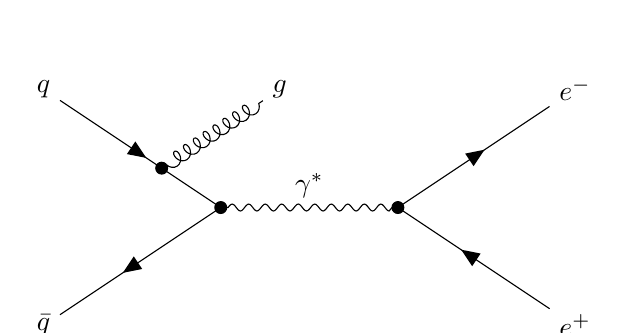
\begin{tikzpicture}
    \begin{feynman}

      \vertex (a1) {\(q\)};
      \vertex[below = 3cm of a1] (a2) {\(\bar{q}\)};

      \vertex[below = 1.5cm of a1] (b1) {};
      \vertex[right = 2.25cm of b1, dot] (v1) {};

      \vertex[right = 2.25cm of v1, dot] (v2) {};
      \vertex[right = 2.25cm of v2] (b2) {};

      \vertex[above = 1.5cm of b2] (a3) {\(e^-\)};
      \vertex[below = 1.5cm of b2] (a4) {\(e^+\)};

      \vertex[dot] (c1) at ($(a1) + (1.5,-1)$) {};
      \vertex (c2) at ($(c1) + (1.5,1)$) {\(g\)};

      \diagram* {
	(a1) -- [fermion] (v1),
	(a2) -- [anti fermion] (v1),

	(v1) -- [photon, edge label = \(\gamma^*\)] (v2),

	(v2) -- [fermion] (a3),
	(v2) -- [anti fermion] (a4),

	(c1) -- [gluon] (c2),
      };
    \end{feynman}
  \end{tikzpicture}
  \qquad \qquad
  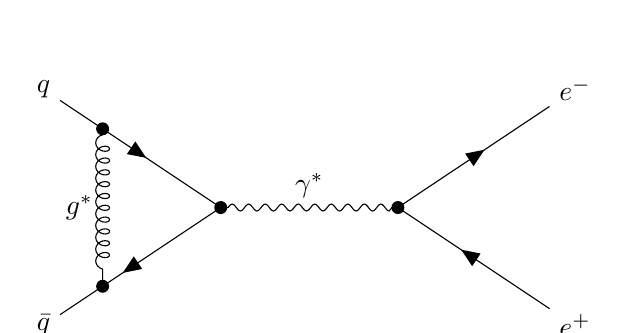
\begin{tikzpicture}
    \begin{feynman}

      \vertex (a1) {\(q\)};
      \vertex[below = 3cm of a1] (a2) {\(\bar{q}\)};

      \vertex[below = 1.5cm of a1] (b1) {};
      \vertex[right = 2.25cm of b1, dot] (v1) {};

      \vertex[right = 2.25cm of v1, dot] (v2) {};
      \vertex[right = 2.25cm of v2] (b2) {};

      \vertex[above = 1.5cm of b2] (a3) {\(e^-\)};
      \vertex[below = 1.5cm of b2] (a4) {\(e^+\)};

      \vertex[dot] (c1) at ($(a1) + (0.75,-0.5)$) {};
      \vertex[dot] (c2) at ($(a2) + (0.75,0.5)$) {};

      \diagram* {
	(a1) -- [fermion] (v1),
	(a2) -- [anti fermion] (v1),

	(v1) -- [photon, edge label = \(\gamma^*\)] (v2),

	(v2) -- [fermion] (a3),
	(v2) -- [anti fermion] (a4),

	(c1) -- [gluon, edge label' = \(g^*\)] (c2),
      };
    \end{feynman}
  \end{tikzpicture}
\end{equation*}
In general, then:
\begin{equation}
  \dd\pcs_{a,b}^{(1)}(p_1 , p_2) = \dd\pcsr_{a,b}(p_1 , p_2) + \dd\pcsv_{a,b}(p_1 , p_2) + \dd\pcspdf_{a,b}(p_1 , p_2)
\end{equation}
where $ \dd\pcsr_{a,b} $ and $ \dd\pcsv_{a,b} $ are the single-real and 1-loop corrections. The additional correction $ \dd\pcspdf_{a,b} $ is due to the collinear renormalization of PDFs.

\section{Singularities in QCD amplitudes}

show how divergences arise in the soft and collinear limits for the real case

cite UV-singularities for the virtual case (link to section about renormalization), then say that IR-singularities cancel when combined with real ones due to the kinoshita-lee-nauenberg theorem

prove the general form of collinear pdf renormalization counterterms












\mainmatter

\part{Differential Geometry}
\pagestyle{body}

\chapter{Manifolds}
\selectlanguage{english}

\section{Topological spaces}

\begin{definition}
  The \textit{topology} $ \mathcal{T} $ of a set $ X $ is a family of subsets of $ X $, i.e. $ \mathcal{T} \subseteq \mathcal{P}(X) $, defined as \textit{open sets}, with the following properties:
  \begin{enumerate}
    \item $ \emptyset,X \in \mathcal{T} $;
    \item $ O_{\alpha},O_{\beta} \in \mathcal{T} \, \Rightarrow\, O_{\alpha}\cap O_{\beta} \in \mathcal{T} $;
    \item $ \{O_{\alpha}\}_{\alpha \in I} \subset \mathcal{T} $ ($ I $ arbitrary index set) $ \Rightarrow \bigcup_{\alpha \in I} O_{\alpha} \in \mathcal{T} $.
  \end{enumerate}
\end{definition}

\begin{definition}
  A \textit{topological space} $ M $ is a set of points, endowed with a topology $ \mathcal{T} $.
\end{definition}

\begin{definition}
  Given a topological space $ (M,\mathcal{T}) $, $ O \in \mathcal{T} $ is a \textit{neighbourhood} of a point $ p \in M $ if $ p \in O $.
\end{definition}

\begin{definition}
  A topological space $ (M,\mathcal{T}) $ is \textit{Hausdorff} if $ \forall p,q \in M \, \exists O_1, O_2 \in \mathcal{T} $ neighbourhoods of $ p $ and $ q $ respectively such that $ O_1 \cap O_2 = \emptyset $.
\end{definition}

\begin{definition}
  A \textit{homeomorphism} between two topological spaces $ (M_1, \mathcal{T}_1) $ and $ (M_2, \mathcal{T}_2) $ is a bijective map $ f : M_1 \rightarrow M_2 $ which is bicontinuous, i.e. both $ f $ and $ f^{-1} $ are continuous: $ f $ is continuous if $ O \in \mathcal{T}_2 \,\Rightarrow\, f^{-1}(O)\in \mathcal{T}_1 $.
\end{definition}

\section{Differentiable Manifolds}

\begin{definition}
  An $ n $-dimensionale \textit{differentiable manifold} $ \mathcal{M} $ is a Hausdorff topological space such that:
  \begin{enumerate}
    \item $ \mathcal{M} $ is locally homeomorphic to $ \R^n $, i.e. $ \forall p\in\mathcal{M} \, \exists O \in \mathcal{T}(\mathcal{M}) : p \in O \land \exists \varphi : O \rightarrow U \in \mathcal{T}(\R^n) $ homeomorphism;
    \item given $ O_{\alpha},O_{\beta} \in \mathcal{T}(\mathcal{M}) : O_{\alpha} \cap O_{\beta} \neq \emptyset $, the corresponding maps $ \varphi_{\alpha} : O_{\alpha} \rightarrow U_{\alpha}, \varphi_{\beta} : O_{\beta} \rightarrow U_{\beta} $ must be \textit{compatible}, i.e. $ \varphi_{\beta} \circ \varphi_{\alpha}^{-1} : \varphi_{\alpha}(O_{\alpha} \cap O_{\beta}) \rightarrow \varphi_{\beta}(O_{\alpha} \cap O_{\beta}) $ and its inverse must be smooth (of $ \mathcal{C}^{\infty} $ class).
  \end{enumerate}
\end{definition}

The maps $ \varphi_{\alpha} $ are called \textit{charts} and a collection of compatible charts is called an \textit{atlas}: a \textit{maximal atlas} $ \mathcal{A} $ is an atlas such that $ \bigcup_{\alpha \in I} O_{\alpha} = \mathcal{M} $. Two atlases are compatible if each chart of one atlas is compatible with every chart of the other: they define the same \textit{differentiable structure} on the manifold.\\
Each chart $ \varphi_{\alpha} $ provides a coordinate system on the region $ O_{\alpha} $: $ \varphi_{\alpha}(p) = \left( x^1(p), \dots, x^{\mu}(p), \dots, x^n(p) \right) $. The \textit{transition functions} $ \varphi_{\beta} \circ \varphi_{\alpha}^{-1} $ are therefore coordinate transformations on overlapping regions.

\begin{example}
  The $ n $-sphere $ \mathbb{S}^n $ is a differentiable manifold.
\end{example}
\begin{example}
  To define a differentiable structure on $ \mathcal{S}^1 $ an atlas of two charts is needed: the standard parametrization $ \theta \in [0, 2\pi) $ is not a well-defined chart because $ [0,2\pi) $ is not an open set in the Euclidean topology of $ \R $, therefore the elimination of a point is necessary; usually, the two charts of the atlas are defined by $ \theta_1 \in (0,2\pi) $, excluding $ (1,0) $ (in the embedding space $ \R^2 $), and $ \theta_2 \in (-\pi,\pi) $, excluding $ (-1,0) $: they are evidently compatible, thus they form a maximal atlas.
\end{example}

\subsection{Maps between manifolds}

Locally mapping $ \mathcal{M} $ to $ \R^n $ allows to import concepts of Analysis from $ \R^n $ to $ \mathcal{M} $.

\begin{definition}
  A function $ f : \mathcal{M} \rightarrow \R $ on a differentiable manifold $ (\mathcal{M},\mathcal{A}) $ is \textit{smooth} if $ f \circ \varphi_{\alpha}^{-1} : U_{\alpha} \rightarrow \R $ is smooth for all charts $ (U_{\alpha},\varphi_{\alpha}) \in \mathcal{A} $.
\end{definition}

\begin{definition}
  A map $ f : \mathcal{M} \rightarrow \mathcal{N} $ between two differentiable manifolds $ (\mathcal{M},\mathcal{A}_1), (\mathcal{N},\mathcal{A}_2) $ is \textit{smooth} if $ \psi_{\alpha_2} \circ f \circ \varphi_{\alpha_1}^{-1} : U_{\alpha_1} \rightarrow V_{\alpha_2} $ is smooth for all charts $ (U_{\alpha_1},\varphi_{\alpha_1}) \in \mathcal{A}_1, (V_{\alpha_2},\varphi_{\alpha_2}) \in \mathcal{A}_2 $.
\end{definition}

\begin{definition}
  A \textit{diffeomorphism} between two differentiable manifolds $ \mathcal{M},\mathcal{N} $ is a smooth homeomorphism $ f : \mathcal{M} \rightarrow \mathcal{N} $.
\end{definition}

\begin{proposition}
  If $ \mathcal{M} $ and $ \mathcal{N} $ are diffeomorphic, then $ \dim_{\R}\mathcal{M} = \dim_{\R}\mathcal{N} $.
\end{proposition}

\begin{example}
  $ \mathbb{S}^7 $ can be covered by multiple incompatible atlases: the resulting manifolds are homeomorphic but not diffeomorphic.
\end{example}

\begin{example}
  $ \R^n $ has a unique differentiable structure for all $ n \in \N $, except for $ n = 4 $: $ \R^4 $ can be covered by infinitely-many incompatible atlases.
\end{example}

\section{Tangent spaces}

The notions of calculus can be defined on a differential manifold $ (\mathcal{M},\mathcal{A}) $ via tangent spaces.

\begin{definition}
  The derivative of a function $ f : \mathcal{M} \rightarrow \R $ at a point $ p \in \mathcal{M} $, covered by the chart $ (\varphi,U) $, is defined as:
  \begin{equation}
    \frac{\pa f}{\pa x^{\mu}}\bigg\vert_p \defeq \frac{\pa (f \circ \varphi^{-1})}{\pa x^{\mu}}\bigg\vert_{\varphi(p)}
    \label{eq:2.1}
  \end{equation}
\end{definition}

Evidently, this definition depends on the choise of coordinates $ x^{\mu} $, thus it depends on the chart.

\subsection{Tangent vectors}

\begin{definition}
  The set of all smooth functions on $ \mathcal{M} $ is denoted by $ \cm $.
\end{definition}

\begin{definition}\label{tang-vec}
  A \textit{tangent vector} to $ \mathcal{M} $ in $ p \in \mathcal{M} $ is an operator $ X_p : \cm \rightarrow \R $ such that:
  \begin{enumerate}
    \item $ X_p(f + g) = X_p(f) + X_p(g) \,\forall f,g \in\cm $;
    \item $ X_p(f) = 0 $ for all constant functions;
    \item $ X_p(fg) = X_p(f)g(p) + f(p)X_p(g) \,\forall f,g \in\cm $.
  \end{enumerate}
\end{definition}

\begin{proposition}
  $ X_p(\alpha f) = \alpha X_p(f) \,\forall \alpha \in \R $.
\end{proposition}
\begin{proof}
  Trivial from conditions 2. and 3. of Def. \ref{tang-vec}.
\end{proof}

It is simple to check that $ \pa_{\mu}\vert_p $ satisfies the conditions of Def. \ref{tang-vec}.

\begin{theorem}
  The set $ T_p\mathcal{M} $ of all tangent vectors at a point $ p\in\mathcal{M} $ forms an $ n $-dimensional space, called \textit{tangent space}, and $ \{\pa_{\mu}\vert_p\}_{\mu = 1,\dots,n} $ is a base of such space.
\end{theorem}
\begin{proof}
  Defining $ f \circ \varphi^{-1} \equiv F : U \subset \mathcal{M} \rightarrow \R $, with $ f : \mathcal{M} \rightarrow \mathcal{M} $ and $ (\varphi,U) \in \mathcal{A} $, it can be proved that, in some neighbourhood of $ p $ (not necessarily $ U $), $ F $ cal always be written as:
  \begin{equation*}
    F(x) = F(x^{\mu}(p)) + \left( x^{\mu} - x^{\mu}(p) \right) F_{\mu}(x)
  \end{equation*}
  for some $ n $ functions $ F_{\mu} $ (ex.: a Taylor series, or more generally $ F(x) = F(0) + x \int_0^1 dt\,F(xt) $). Applying $ \pa_{\mu}\vert_{x(p)} $:
  \begin{equation*}
    \frac{\pa F}{\pa x^{\mu}}\bigg\vert_{x(p)} = F_{\mu}(x(p))
  \end{equation*}
  Defining $ f_{\mu} \equiv F_{\mu} \circ \varphi $, for any $ q \in \mathcal{M} $ in an appropriate neighbourhood of $ p $:
  \begin{equation*}
    f(q) = f(p) + \left( x^{\mu}(q) - x^{\mu}(p) \right) f_{\mu}(q)
  \end{equation*}
  Moreover, remembering Eq. \ref{eq:2.1}:
  \begin{equation*}
    f_{\mu}(p) = F_{\mu} \circ \varphi(p) = F_{\mu}(x(p)) = \frac{\pa F}{\pa x^{\mu}}\bigg\vert_{x(p)} = \frac{\pa f}{\pa x^{\mu}}\bigg\vert_p
  \end{equation*}
  Using these facts, the action of a tangent vector can be written explicitly:
  \begin{equation*}
    \begin{split}
      X_p(f)
      &= X_p\left( f(p) + \left( x^{\mu} - x^{\mu}(p) \right) f_{\mu} \right)\\
      &= X_p\left( f(p) \right) + X_p\left( \left( x^{\mu} - x^{\mu}(p) \right) \right) f_{\mu}(p) + \left( x^{\mu} - x^{\mu}(p) \right)(p) X_p\left( f_{\mu} \right)\\
      &= X_p\left( x^{\mu} \right) f_{\mu}(p)
    \end{split}
  \end{equation*}
  because $ f(p) $ is a constant and $ \left( x^{\mu} - x^{\mu}(p) \right)(p) = x^{\mu}(p) - x^{\mu}(p) = 0 $. Therefore, remembering the expression for $ f_{\mu}(p) $:
  \begin{equation*}
    X_p = X_p(x^{\mu}) \frac{\pa}{\pa x^{\mu}}\bigg\vert_p \equiv X^{\mu} \frac{\pa}{\pa x^{\mu}}\bigg\vert_p
  \end{equation*}
  Thus, $ T_p\mathcal{M} = \lspan\{\pa_{\mu}\vert_p\} $. To check for linear independence, suppose $ \alpha = \alpha^{\mu} \pa_{\mu}\vert_p \equiv 0 $: acting on $ f = x^{\nu} $, it gives $ \alpha(f) = \alpha_{\mu} \pa_{\mu}(x^{\nu})\vert_p = \alpha_{\nu} = 0 $. This concludes the proof.
\end{proof}

\subsubsection{Changing coordinates}

Although $ \pa_{\mu}\vert_p $ depends on the choice of coordinates (it is a \textit{coordinate basis}), the existence of $ X_p $ is independent of that choice.\\
If two different charts $ (\varphi,U),(\tilde{\varphi},V) $ intersect in a neighbourhood of $ p \in U \cap V $, the transition from $ x^{\mu} $ to $ y^{\mu} $ can be expressed as:
\begin{equation}
  X_p(f) = X^{\mu} \frac{\pa f}{\pa x^{\mu}}\bigg\vert_p = X^{\mu} \frac{\pa y^{\nu}}{\pa x^{\mu}}\bigg\vert_{\varphi(p)} \frac{\pa f}{\pa y^{\nu}}\bigg\vert_p
\end{equation}
This equation can have two interpretations: the alibi interpretation:
\begin{equation}
  \frac{\pa}{\pa x^{\mu}}\bigg\vert_p = \frac{\pa y^{\nu}}{\pa x^{\mu}}\bigg\vert_{\varphi(p)} \frac{\pa}{\pa y^{\nu}}\bigg\vert_p
  \label{eq:2.3}
\end{equation}
and the alias interpretation:
\begin{equation}
  \tilde{X}^{\nu} = X^{\mu} \frac{\pa y^{\nu}}{\pa x^{\mu}}\bigg\vert_{\varphi(p)}
  \label{eq:2.4}
\end{equation}
Components of vectors which transform this way are called \textit{contravariant}.

\subsubsection{Curves}

Consider a smooth curve on $ \mathcal{M} $, i.e. a smooth map $ \sigma : I \in \mathcal{T}(\R) \rightarrow \mathcal{M} $, parametrized as $ \sigma(t) : \sigma(0) = p \in \mathcal{M} $; with a given chart $ (\varphi,U) $, this curve becomes $ \varphi \circ \sigma : I \rightarrow \R^n $, parametrized by $ x^{\mu}(t) $.
The \textit{tangent vector} to the curve in $ p $ is:
\begin{equation}
  X_p = \frac{dx^{\mu}(t)}{dt}\bigg\vert_{t=0} \frac{\pa}{\pa x^{\mu}}\bigg\vert_p
  \label{eq:2.5}
\end{equation}
This operator, applied to a function $ f \in\cm $, calculates the directional derivative of $ f $ along the curve. It can be showed that every tangent vector can be written as in Eq. \ref{eq:2.5}, therefore the tangent space is literally the space of all possible tangents to curves passing through $ p $.\\
It must be noted that tangent spaces at different points are entirely different spaces: there's no way to directly compare vectors between them.

\subsection{Vector fields}

\begin{definition}
  A \textit{vector field} $ X $ is a smooth map $ X : p \in \mathcal{M} \mapsto X_p \in T_p\mathcal{M} $. It can also be viewed as a smooth map $ X : \cm \rightarrow \cm $, as $ (X(f))(p) = X_p(f) \in \R $.
\end{definition}

\begin{definition}
  The space of all vector fields on $ \mathcal{M} $ is denoted by $ \xm $.
\end{definition}

Given a chart $ (\varphi,U) $, a vector field $ X $ can be expressed as:
\begin{equation}
  X = X^{\mu} \frac{\pa}{\pa x^{\mu}}
  \label{eq:2.6}
\end{equation}
with $ X^{\mu} \in \cm $. This expression is only defined on $ U $.

\subsubsection{Lie brakets}

Given two vector fields $ X,Y \in\xm $, their product is clearly not a vector field, as it does not satisfy Leibniz rule:
\begin{equation*}
  XY(fg) = XY(f) g + Y(f) X(g) + X(f) Y(g) + f XY(g) \neq XY(f) g + f XY(g)
\end{equation*}
where $ XY(f) \equiv X(Y(f)) $.

\begin{definition}
  Given two vector fields $ X,Y \in\xm $, their \textit{commutator} (or \textit{Lie bracket}) is defined as:
  \begin{equation}
    \left[ X,Y \right](f) = XY(f) - YX(f)
    \label{eq:2.7}
  \end{equation}
\end{definition}

With a given chart:
\begin{equation*}
  \begin{split}
    \left[ X,Y \right](f)
    &= X^{\mu} \frac{\pa}{\pa x^{\mu}} \left( Y^{\nu} \frac{\pa f}{\pa x^{\nu}} \right) - Y^{\mu} \frac{\pa}{\pa x^{\mu}} \left( X^{\nu} \frac{\pa f}{\pa x^{\nu}} \right)\\
    &= \left( X^{\mu} \frac{\pa Y^{\nu}}{\pa x^{\mu}} - Y^{\mu} \frac{\pa X^{\nu}}{\pa x^{\mu}} \right) \frac{\pa f}{\pa x^{\nu}}
  \end{split}
\end{equation*}
therefore:
\begin{equation}
  \left[ X,Y \right] = \left( X^{\mu} \frac{\pa Y^{\nu}}{\pa x^{\mu}} - Y^{\mu} \frac{\pa X^{\nu}}{\pa x^{\mu}} \right) \frac{\pa}{\pa x^{\nu}}
  \label{eq:2.8}
\end{equation}

\begin{theorem}[Jacobi]
  Given $ X,Y,Z \in\xm $, the \textit{Jacobi identity} holds:
  \begin{equation}
    \left[ X, \left[ Y,Z \right] \right] + \left[ Y, \left[ Z,X \right] \right] + \left[ Z, \left[ X,Y \right] \right] = 0
    \label{eq:2.9}
  \end{equation}
\end{theorem}

\begin{proposition}
  $ \xm $ is a \textit{Lie algebra}.
\end{proposition}

\subsubsection{Integral curves}

\begin{definition}
  A \textit{flow} on $ \mathcal{M} $ is a one-parameter family of diffeomorphisms $ \sigma_t : \mathcal{M} \rightarrow \mathcal{M} $, labelled by $ t\in\R $, with group structure: $ \sigma_0 = \id_{\mathcal{M}} $ and $ \sigma_s \circ \sigma_t = \sigma_{s+t} $, thus $ \sigma_{-t} = \sigma_t^{-1} $.
\end{definition}

Such flows give rise to streamlines on the manifold: these streamlines are required to be smooth.
Defining $ x^{\mu}(\sigma_t) \equiv x^{\mu}(t) $, a vector field can be defined by the tangent to the streamlines at each point on the manifold:
\begin{equation}
  X^{\mu}(x^{\mu}(t)) = \frac{dx^{\mu}(t)}{dt}
  \label{eq:2.10}
\end{equation}
The inverse reasoning is also possible.

\begin{definition}
  Given a vector field $ X \in\xm $, streamlines described by Eq. \ref{eq:2.10} are called \textit{integral curves} generated by $ X $.
\end{definition}

\begin{proposition}
  The \textit{infinitesimal flow} generated by $ X \in\xm $ is:
  \begin{equation}
    x^{\mu}(t) = x^{\mu}(0) + tX^{\mu}(x(t)) + o(t)
    \label{eq:2.11}
  \end{equation}
\end{proposition}

\begin{definition}
  A vector field which generates a flow defined for all $ t \in \R $ is called \textit{complete}.
\end{definition}

\begin{theorem}
  If $ \mathcal{M} $ is compact, then all $ X \in \xm $ are complete.
\end{theorem}

\begin{example}
  On $ \mathbb{S}^2 $, the flow generated by $ X = \pa_{\phi} $ is described by $ \dot{\phi} = 1, \dot{\theta} = 0 $, thus $ \theta(t) = \theta_0 $ and $ \phi(t) = \phi_0 + t $: the flow lines are lines of constant latitude.
\end{example}

\subsection{Lie derivative}

Defining calculus for vector fields requires a way to compare vectors of different tangent spaces.

\begin{definition}
  Given a diffeomorphism between two manifolds $ \varphi : \mathcal{M} \rightarrow \mathcal{N} $ and a function $ f : \mathcal{N} \rightarrow \R $, the \textit{pull-back} of $ f $ is the function $ \varphi^*f : \mathcal{M} \rightarrow \R $ such that $ \varphi^*f(p) = f(\varphi(p)) $.
\end{definition}

\begin{definition}
  Given a diffeomorphism between two manifolds $ \varphi : \mathcal{M} \rightarrow \mathcal{N} $ and a vector field $ X \in \xm $, the \textit{push-forward} of $ X $ is the vector field $ \varphi_*X \in \mathfrak{X}(\mathcal{N}) $ such that $ \varphi_*X(f) = X(\varphi^*f) $.
\end{definition}

This last equality must be evaluated at the appropriate points: $ [ \varphi_*X(f) ](\varphi(p)) = [ X(\varphi^*f) ](p) $.\\
With the appropriate charts on $ \mathcal{M} $ and $ \mathcal{N} $, the definitions above can be rewritten with coordinates:
\begin{equation}
  \varphi^*f(x) = f(y(x))
  \label{eq:2.12}
\end{equation}
\begin{equation}
  \varphi_*X(f) = X^{\mu} \frac{\pa f(y(x))}{\pa x^{\mu}} = X^{\mu} \frac{\pa y^{\alpha}}{\pa x^{\mu}} \frac{\pa f(y)}{\pa y^{\alpha}}
  \label{eq:2.13}
\end{equation}

The notions of pull-back and push-forward allow to compare tangent vectors at neighbouring points and, in particular, to define the derivative along a vector field.

\begin{definition}
  Given a function $ f : \mathcal{M} \rightarrow \R $ and a vector field $ X \in\xm $, the derivative of $ f $ along $ X $ (called \textit{Lie derivative}) is defined as:
  \begin{equation}
    \ld_X f(x) \defeq \lim_{t \rightarrow 0} \frac{f(\sigma_t(x)) - f(x)}{t} = \frac{df(\sigma_t(x))}{dt}\bigg\vert_{t=0}
    \label{eq:2.14}
  \end{equation}
  where $ \sigma_t $ is the flow generated by $ X $.
\end{definition}

\begin{proposition}
  $ \ld_X f = X(f) $.
\end{proposition}
\begin{proof}
  $ \ld_X f = \frac{df(\sigma_t)}{dt} = \frac{\pa f}{\pa x^{\mu}} \frac{dx^{\mu}(t)}{dt} = X^{\mu} \frac{\pa f}{\pa x^{\mu}} = X(f) $.
\end{proof}

\begin{definition}
  Given two vector fields $ X,Y \in\xm $, the \textit{Lie derivative} of $ Y $ along $ X $ is defined as:
  \begin{equation}
    \ld_X Y_p \defeq \lim_{t \rightarrow 0} \frac{((\sigma_{-t})_*Y)_p - Y_p}{t}
    \label{eq:2.15}
  \end{equation}
  where $ \sigma_t $ is the flow generated by $ X $.
\end{definition}

The use of the inverse flow $ \sigma_{-t} $ is necessary because to evaluate the vector field $ \ld_X Y $ at the point $ p \in \mathcal{M} $, the tangent vector $ Y_{\sigma_t(p)} \in T_{\sigma_t(p)}\mathcal{M} $ must be $ \virgolette{pushed-back} $ to $ T_p\mathcal{M} = T_{\sigma_0(p)}\mathcal{M} $.\\
With $ t \rightarrow 0 $, the infinitesimal flow $ \sigma_{-t} $ is, according to Eq. \ref{eq:2.11}, $ x^{\mu}(t) = x^{\mu}(0) - tX^{\mu} + o(t) $, therefore the Lie derivative of base tangent vectors can be expressed as:
\begin{equation}
  (\sigma_{-t})_* \pa_{\mu} = \frac{\pa x^{\nu}(t)}{\pa x^{\mu}} \frac{\pa}{\pa x^{\nu}(t)} = \left( \delta^{\nu}_{\mu} - t \frac{\pa X^{\nu}}{\pa x^{\mu}} + o(t) \right) \pa_{\nu}(t)
  \quad\Longrightarrow\quad
  \ld_X \pa_{\mu} = - \frac{\pa X^{\nu}}{\pa x^{\mu}} \pa_{\nu}
  \label{eq:2.16}
\end{equation}

\begin{proposition}
  $ \ld_X Y = \left[ X,Y \right] $.
\end{proposition}
\begin{proof}
  $ \ld_X Y = \ld_X (Y^{\mu} \pa_{\mu}) = \left( \ld_X Y^{\mu} \right) \pa_{\mu} + Y^{\mu} \left( \ld_X \pa_{\mu} \right) = X^{\nu} \frac{\pa Y^{\mu}}{\pa x^{\nu}} \pa_{\mu} - Y^{\mu} \frac{\pa X^{\nu}}{\pa x^{\mu}} \pa_{\nu} = \left[ X,Y \right] $.
\end{proof}
\begin{proposition}
  $ \ld_X \ld_Y Z - \ld_Y \ld_X Z = \ld_{\left[ X,Y \right]} Z $.
\end{proposition}
\begin{proof}
  Trivial with Jacobi identity.
\end{proof}

\section{Tensors}

\subsection{Dual Spaces}

\begin{definition}
  Given a vector space $ V $, its \textit{dual} $ V^* $ is the space of all linear maps $ f : V \rightarrow \R $.
\end{definition}

Given a basis $ \{\ve{e}_{\mu}\}_{\mu = 1,\dots,n} $ of $ V $, its \textit{dual basis} $ \{\ve{f}^{\mu}\}_{\mu=1,\dots,n} $ of $ V^* $ can be defined by:
\begin{equation}
  \ve{f}^{\nu}(\ve{e}_{\mu}) = \delta^{\nu}_{\mu}
  \label{eq:2.17}
\end{equation}
A general vector in $ V $ can be written as $ X = X^{\mu} \ve{e}_{\mu} $, thus according to Eq. \ref{eq:2.17} $ X^{\mu} = \ve{f}^{\mu}(X) $.

\begin{proposition}
  The map $ f : \ve{e}_{\mu} \mapsto \ve{f}^{\mu} $ is an isomorphism between $ V $ and $ V^* $.
\end{proposition}

This isomorphism, however, is basis-dependent.

\begin{proposition}
  $ \dim_{\R}V = \dim_{\R}V^* $.
\end{proposition}

\begin{proposition}
  $ (V^*)^* = V $.
\end{proposition}
\begin{proof}
  The natural isomorphism between $ (V^*)^* $ and $ V $ is basis-independent: suppose $ X \in V $ and $ \omega \in V^* $, so that $ \omega(X) \in \R $; $ X $ can be viewed as $ X \in (V^*)^* $ by setting $ V(\omega) \equiv \omega(V) $.
\end{proof}

\subsection{Cotangent vectors}

\begin{definition}
  Given a differentiable manifold $ (\mathcal{M},\mathcal{A}) $ and a point $ p \in \mathcal{M} $, the \textit{cotangent space} to $ \mathcal{M} $ at $ p $ is defined as $ T^*_p\mathcal{M} \defeq (T_p\mathcal{M})^* $.
\end{definition}

Elements of $ T^*_p\mathcal{M} $ are called \textit{cotangent vectors} (or \textit{covectors}).

\begin{definition}
  A \textit{covector field} (or \textit{1-form}) is a smooth map $ \omega : p \in \mathcal{M} \mapsto \omega_p \in T^*_p\mathcal{M} $. It can also be viewed as a smooth map $ \omega : \xm \rightarrow \cm $, as $ (\omega(X))(p) = \omega_p(X_p) \in \R $.
\end{definition}

\begin{definition}
  The space of all 1-forms on $ \mathcal{M} $ is denoted by $ \lm{1} $.
\end{definition}

\begin{proposition}
  $ \{dx^{\mu}\}_{\mu = 1,\dots,n} $ is a basis of $ \lm{1} $ dual to the basis $ \{\pa_{\mu}\}_{\mu = 1,\dots,n} $ of $ \xm $.
\end{proposition}
\begin{proof}
  Consider $ f \in \cm $ and define $ df \in \lm{1} $ by $ df(X) = X(f) $: taking $ f = x^{\mu} $ and $ X = \pa_{\mu} $, $ df(X) = \pa_{\nu}(x^{\mu}) = \delta^{\mu}_{\nu} $, therefore $ \{dx^{\mu}\}_{\mu = 1,\dots,n} $ is the dual basis of $ \lm{1} $.
\end{proof}

This is also confirmed by $ df = \frac{\pa f}{\pa x^{\mu}} dx^{\mu} $. These are coordinate basis: in fact, given two different charts $ (\varphi,U), (\tilde{\varphi},V) $:
\begin{equation}
  dy^{\mu} = \frac{dy^{\mu}}{dx^{\nu}}dx^{\nu}
  \label{eq:}
\end{equation}
which is the inverse of Eq. \ref{eq:2.3} (not evaluated at a specific point). This ensures that:
\begin{equation*}
  dy^{\mu}\left( \frac{\pa}{\pa y^{\nu}} \right) = \frac{\pa y^{\mu}}{\pa x^{\alpha}} \frac{\pa x^{\beta}}{\pa y^{\nu}} dx^{\alpha}\left( \frac{\pa}{\pa x^{\beta}} \right) = \frac{\pa y^{\mu}}{\pa x^{\alpha}} \frac{\pa x^{\alpha}}{\pa y^{\nu}} = \delta^{\mu}_{\nu}
\end{equation*}
A 1-form $ \omega \in \lm{1} $ can thus be expressed both as $ \omega = \omega_{\mu} dx^{\mu} = \tilde{\omega}_{\mu} dx^{\mu} $, with:
\begin{equation}
  \tilde{\omega}_{\omega} = \frac{\pa x^{\nu}}{\pa y^{\mu}} \omega_{\nu}
  \label{eq:2.19}
\end{equation}
Components of 1-forms which transform this way are called \textit{covariant}.

\begin{definition}
  Given a diffeomorphism between two manifolds $ \varphi : \mathcal{M} \rightarrow \mathcal{N} $ and a 1-form $ \omega \in \Lambda^1(\mathcal{N}) $, the \textit{pull-back} of $ \omega $ is the 1-form $ \varphi^*\omega \in \lm{1} $ such that $ \varphi^*\omega(X) = \omega(\varphi_*X) $.
\end{definition}

With the appropriate charts on $ \mathcal{M} $ and $ \mathcal{N} $, the definition above can be rewritten with coordiantes:
\begin{equation}
  \varphi^*\omega = \omega_{\alpha} \frac{\pa y^{\alpha}}{\pa x^{\mu}} dx^{\mu}
  \label{eq:2.20}
\end{equation}

\begin{definition}
  Given a vector field $ X \in \xm $ and a 1-form $ \omega \in \lm{1} $, the \textit{Lie derivative} of $ \omega $ along $ X $ is defined as:
  \begin{equation}
    \ld_X \omega \defeq_{t \rightarrow 0} \frac{(\sigma_t^* \omega)_p - \omega_p}{t}
    \label{eq:2.21}
  \end{equation}
  where $ \sigma_t $ is the flow generated by $ X $.
\end{definition}

In contranst with the Lie derivative of a vector field, which pushes forward with $ \sigma_{-t} $ (i.e. pushes back), the Lie derivative of a 1-form pulls back with $ \sigma_t $: this results in the difference of a minus sign with respect to Eq. \ref{eq:2.16}, giving:
\begin{equation}
  \ld_X dx^{\mu} = \frac{\pa X^{\mu}}{\pa x^{\nu}} dx^{\nu}
  \label{eq:2.22}
\end{equation}
Therefore, on a general 1-form $ \omega = \omega_{\mu} dx^{\mu} $:
\begin{equation}
  \ld_X \omega = \left( X^{\nu} \pa_{\nu} \omega_{\mu} + \omega_{\nu} \pa_{\mu} X^{\nu} \right) dx^{\mu}
  \label{eq:2.23}
\end{equation}

\subsection{Tensor fields}












\chapter{Riemannian Geometry}
\selectlanguage{english}

\section{Metric manifolds}

\begin{definition}
  A \textit{metric} $ g $ is a (0,2) tensor field on a manifold $ \mathcal{M} $ that is:
  \begin{enumerate}
    \item symmetric: $ g(X,Y) = g(Y,X) $;
    \item non-degenerate: $ \exists p \in \mathcal{M} : g(X,Y)\vert_p = 0 \,\forall Y \in T_p \mathcal{M} \,\Rightarrow\, X_p = 0 $.
  \end{enumerate}
\end{definition}

\begin{definition}
  A \textit{metric manifold} $ (\mathcal{M},g) $ is a manifold equipped with a metric.
\end{definition}

With a choice of coordinates, the metric can be written as:
\begin{equation}
  g = g_{\mu \nu}(x) dx^{\mu} \otimes dx^{\nu}
  \label{eq:3.1}
\end{equation}
where:
\begin{equation}
  g_{\mu \nu} = g\left( \frac{\pa}{\pa x^{\mu}}, \frac{\pa}{\pa x^{\nu}} \right)
  \label{eq:3.2}
\end{equation}
It is often written also as $ ds^2 = g_{\mu \nu}(x) dx^{\mu} dx^{\nu} $. The matrix $ g_{\mu \nu}(x) \in \R^{n \times n} $ is symmetric, and there's always a choice of basis on each tangent space such that this matrix is diagonal: the non-degeneracy condition implies that none of the diagonal elements vanish.

\begin{proposition}
  The \textit{signature} of a metric, i.e. the number of negative entries when diagonalized, is independent on the choice of basis.
\end{proposition}
\begin{proof}
  From Sylvester's theorem of inertia.
\end{proof}

\paragraph{Riemannian manifolds}

\begin{definition}
  A \textit{Riemannian manifold} $ (\mathcal{M},g) $ is a manifold equipped with a metric with totally-positive signature.
\end{definition}

\begin{example}
  The Euclidean space $ \R^n $, equipped with the metric $ g_{\mu \nu} = \delta_{\mu \nu} $ (in Cartesian coordinates), is a Riemannian manifold.
\end{example}

\begin{definition}
  Given a Riemannian manifold $ (\mathcal{M},g) $ and $ X \in \xm $, the \textit{length} of $ X $ at $ p \in \mathcal{M} $ is:
  \begin{equation}
    \abs{X_p} \defeq \sqrt{g(X,X)\vert_p}
    \label{eq:3.3}
  \end{equation}
  Given $ Y \in \xm $, the \textit{angle} between $ X $ and $ Y $ at $ p \in \mathcal{M} $ is:
  \begin{equation}
    \cos \theta \defeq \frac{g(X,Y) \vert_p}{\abs{X_p} \abs{Y_p}}
    \label{eq:3.4}
  \end{equation}
\end{definition}

This can be generalized to distances between points on a curve $ \sigma : \mathcal{\R} \rightarrow \mathcal{M} $:
\begin{equation}
  d(p,q) = \int_a^b dt \sqrt{g(X,X)\vert_{\sigma(t)}}
  \label{eq:3.5}
\end{equation}
where $ \sigma(a) = p $, $ \sigma(b) = q $ and $ X $ is the tangent vector field of the curve. With parametrization $ x^{\mu}(t) $, the tangent vector has components $ X^{\mu} = \frac{dx^{\mu}}{dt} $, thus:
\begin{equation}
  d(p,q) = \int_a^b dt \sqrt{g_{\mu \nu}(x) \frac{dx^{\mu}}{dt} \frac{dx^{\nu}}{dt}}
  \label{eq:3.6}
\end{equation}
It is important to note that this distance is independent of the parametrization.

\paragraph{Lorentzian manifolds}

\begin{definition}
  A \textit{Lorentzian manifold} $ (\mathcal{M},g) $ is a manifold equipped with a metric which has a signature with a single negative sign.
\end{definition}

\begin{example}
  The simplest Lorentzian manifold is $ \R^n $ with the \textit{Minkowski metric}:
  \begin{equation}
    \eta = - dx^0 \otimes dx^0 + dx^1 \otimes dx^1 + \dots + dx^{n-1} \otimes dx^{n-1}
    \label{eq:3.7}
  \end{equation}
  Its components are $ \eta_{\mu \nu} = \diag (-1,+1,\dots,+1) $, thus this is a Lorentzian manifold.
\end{example}

On a general Lorentzian manifold, at any point $ p \in \mathcal{M} $ it is always possible to choose an orthonormal basis $ \{e_{\mu}\}_{\mu = 0,\dots,n-1} $ of $ T_p \mathcal{M} $ such that $ g_{\mu \nu} \vert_p = \eta_{\mu \nu} $: this fact is closely related to the equivalence principle. Consider a different basis $ \tilde{e}_{\mu} = \tensor{\Lambda}{^\nu _\mu} e_{\nu} $: the condition for it to leave the Minkowski metric unchanged is:
\begin{equation}
  \eta_{\mu \nu} = \tensor{\Lambda}{^\rho _\mu} \tensor{\Lambda}{^\sigma _\nu} \eta_{\rho \sigma}
  \label{eq:3.8}
\end{equation}
This is the defining equation of a Lorentz transformation: on a Lorentzian manifold, the basic features of special relativity are locally recovered. Thus, other ideas from special relativity can be imported.

\begin{definition}
  Given a Lorentzian manifold $ (\mathcal{M},g) $ and $ X \in \xm $, at $ p \in \mathcal{M} $ the vector field is said to be:
  \begin{itemize}
    \item \textit{timelike} if $ g(X_p,X_p) < 0 $;
    \item \textit{null} if $ g(X_p,X_p) = 0 $;
    \item \textit{spacelike} if $ g(X_p,X_p) > 0 $.
  \end{itemize}
\end{definition}

At each point $ p \in \mathcal{M} $ it is possible to draw \textit{lightcones}, i.e. the null tangent vectors at that point, which are past-directed or future-directed: these lightcones vary smoothly as the point is varied smoothly on the manifold, elucidating the causal structure of spacetime.\\
The distance between two points on a curve depends on the nature of the tangent vector field of the curve: a \textit{timelike curve} is a curve whose tangent vector field is everywhere timelike, and analogously for the other cases. The distance on a spacelike curve is defined as in Eq. \ref{eq:3.5}, while that on a timelike curve gets a negative sign in the square root. With parametrization $ x^{\mu}(t) $, it is possible to define the \textit{proper time} on a timelike curve as:
\begin{equation}
  \tau = \int_a^b dt \sqrt{- g_{\mu \nu}(x) \frac{dx^{\mu}}{dt} \frac{dx^{\nu}}{dt}}
  \label{eq:3.9}
\end{equation}
This is precisely the action of a free particle moving in spacetime.

\subsection{Metric properties}

The metric defines a natural isomorphism between vectors and covectors.

\begin{proposition}\label{metric-isom}
  Given a metric manifold $ (\mathcal{M},g) $, the metric defines for each $ p \in \mathcal{M} $ a \textit{natural isomorphism} $ g : X_p \in T_p \mathcal{M} \rightarrow \omega_p \in T^*_p \mathcal{M} : \omega_p(Y_p) = g(X_p,Y_p) \,\forall Y_p \in T_p \mathcal{M} $.
\end{proposition}

In a chosen coordinate basis, the vector $ X = X^{\mu} \pa_{\mu} $ is mapped to the one-form $ X = X_{\mu} dx^{\mu} $, thus the following identity holds:
\begin{equation}
  X_{\mu} = g_{\mu \nu} X^{\nu}
  \label{eq:3.10}
\end{equation}
Being $ g $ non-degenerate, the matrix $ g_{\mu \nu} $ is invertible, with inverse $ g^{\mu \nu} $ such that:
\begin{equation}
  g^{\mu \nu} g_{\nu \rho} = \delta^{\mu}_{\rho}
  \label{eq:3.11}
\end{equation}
Its elements are the components of a (2,0) symmetric tensor $ \hat{g} \defeq g^{\mu \nu} \pa_{\mu} \otimes \pa_{\nu} $, which defines the inverse of the natural isomorphism in Prop. \ref{metric-isom}:
\begin{equation}
  X^{\mu} = g^{\mu \nu} X_{\nu}
  \label{eq:3.12}
\end{equation}
The metric also defines a natural volume form on the manifold.

\begin{definition}
  Given an $ n $-dimensional metric manifold $ (\mathcal{M},g) $, the \textit{volume form} is the top-form:
  \begin{equation}
    v \defeq \sqg\, dx^1 \wedge \dots \wedge dx^n
    \label{eq:3.13}
  \end{equation}
  where $ \tens{g} \defeq \abs{\det g_{\mu \nu}} $.
\end{definition}

\begin{proposition}
  The volume form is basis-independent.
\end{proposition}
\begin{proof}
  Consider a new set of coordinates $ y^{\mu} $ such that $ dx^{\mu} = \tensor{A}{^\mu _\nu} dy^{\nu} $, where $ \tensor{A}{^\mu _\nu} = \frac{\pa x^{\mu}}{\pa y^{\nu}} $. In general:
  \begin{equation*}
    dx^1 \wedge \dots \wedge dx^n = \tensor{A}{^1 _{\mu_1}} \dots \tensor{A}{^n _{\mu_n}} dy^{\mu_1} \wedge \dots \wedge dy^{\mu_n}
  \end{equation*}
  Recalling the anti-symmetry of the wedge product and the definition of determinant, this can be rewritten as:
  \begin{equation*}
    dx^1 \wedge \dots \wedge dx^n = \sum_{\pi \in S^n} \sgn{\pi} \tensor{A}{^1 _{\pi(1)}} \dots \tensor{A}{^n _{\pi(n)}} dy^1 \wedge \dots \wedge dy^n = \det A \, dy^1 \wedge \dots \wedge dy^n
  \end{equation*}
  Note the Jacobian factor which arises when changing the measure. On the other hand:
  \begin{equation*}
    g_{\mu \nu} = \frac{\pa y^{\rho}}{\pa x^{\mu}} \frac{\pa y^{\sigma}}{\pa x^{\nu}} \tilde{g}_{\rho \sigma} = \tensor{(A^{-1})}{^\rho _\mu} \tensor{(A^{-1})}{^\sigma _\nu} \tilde{g}_{\rho \sigma}
    \quad \Rightarrow \quad
    \det g_{\mu \nu} = \frac{\det \tilde{g}_{\mu \nu}}{\left( \det A \right)^2}
  \end{equation*}
  The factors $ \det A $ and $ \left( \det A \right)^{-1} $ cancel, thus yielding the thesis.
\end{proof}

The volume form can be rewritten as:
\begin{equation}
  v = \frac{1}{n!} v_{\mu_1 \dots \mu_n} dx^{\mu_1} \wedge \dots \wedge dx^{\mu_n} \equiv \frac{1}{n!} \sqg\, \epsilon_{\mu_1 \dots \mu_n} dx^{\mu_1} \wedge \dots \wedge dx^{\mu_n}
  \label{eq:3.14}
\end{equation}
where $ \epsilon_{\mu_1 \dots \mu_n} $ is the totally-antisymmetric $ n $-dimensional symbol (generalization of the Levi-Civita symbol). $ \epsilon_{\mu_1 \dots \mu_n} $ cannot be considered a proper tensor, as its components are always $ +1,-1,0 $ indipendently if the indices are covariant or contravariant: it is, in fact, a \textit{tensor density}, i.e. a tensor divided by $ \sqg $. It can be shown that:
\begin{equation}
  v^{\mu_1 \dots \mu_n} = g^{\mu_1 \nu_1} \dots g^{\mu_n \nu_n} v_{\mu_1 \dots \mu_n} = \sigma \frac{1}{\sqg} \epsilon^{\mu_1 \dots \mu_n}
  \label{eq:3.15}
\end{equation}
where $ \sigma $ is the sign of the signature (ex.: $ \sigma = +1 $ for Riemannian manifolds and $ \sigma = -1 $ for Lorentzian manifolds).
As notation, the integral of a generic function $ f $ on $ \mathcal{M} $ is denoted as:
\begin{equation}
  \int_{\mathcal{M}} f v \equiv \int_{\mathcal{M}} d^n x \,\sqg f
  \label{eq:3.16}
\end{equation}

\subsubsection{Hodge theory}

\begin{definition}
  Given an $ n $-dimensional oriented metric manifold $ (\mathcal{M},g) $, the \textit{Hodge dual} is defined as the map $ \star : \lm{p} \rightarrow \lm{n-p} : \omega \mapsto \star\, \omega $ such that:
  \begin{equation}
    \star\, \omega_{\mu_1 \dots \mu_{n-p}} \defeq \frac{1}{(n-p)!} \sqg\, \epsilon_{\mu_1 \dots \mu_{n-p} \nu_1 \dots \nu_p} \omega^{\nu_1 \dots \nu_p}
    \label{eq:3.17}
  \end{equation}
\end{definition}

In this section, the orientedness and $ n $-dimensionality of the manifold are implied.

\begin{proposition}
  The Hodge dual is basis-independent.
\end{proposition}

It is useful to state a lemma for future calculations.

\begin{lemma}
  $ v^{\mu_1 \dots \mu_p \rho_1 \dots \rho_{n-p}} v_{\nu_1 \dots \nu_p \rho_1 \dots \rho_{n-p}} = \sigma p! (n-p)! \delta^{\mu_1}_{[\nu_1} \dots \delta^{\mu_p}_{\nu_p]} $.
\end{lemma}

\begin{proposition}\label{hodge-hodge}
  $ \star \left( \star\, \omega \right) = \sigma \left( -1 \right)^{p (n-p)} \omega $.
\end{proposition}

The Hodge dual defines an inner product on each $ \lm{p} $:
\begin{equation}
  \braket{\omega, \eta} \defeq \int_{\mathcal{M}} \omega \wedge \star\, \eta
  \label{eq:3.18}
\end{equation}
This allows to define operators and their adjoints on the form spaces.

\begin{proposition}
  Given a metric manifold $ (\mathcal{M},g) $ and two forms $ \omega \in \lm{p}, \alpha \in \lm{p-1} $, then:
  \begin{equation}
    \braket{d\alpha,\omega} = \braket{\alpha,d^{\dagger}\omega}
    \label{eq:3.19}
  \end{equation}
  where the adjoint of the exterior derivative $ d^{\dagger} : \lm{p} \rightarrow \lm{p-1} $ is defined as:
  \begin{equation}
    d^{\dagger} \defeq \sigma \left( -1 \right)^{np + n -1} \star d \, \star
    \label{eq:3.20}
  \end{equation}
\end{proposition}
\begin{proof}
  To simplify the proof, consider a closed manifold; then, from Stokes' theorem and Eq. \ref{eq:2.38}:
  \begin{equation*}
    0 = \int_{\mathcal{M}} d ( \alpha \wedge \star\, \omega ) = \braket{d\alpha, \omega} + \int_{\mathcal{M}} \left( -1 \right)^{p-1} \alpha \wedge d \star \omega
  \end{equation*}
  The second term is proportional to $ \braket{\alpha, \star\, d \star \omega} $: to determine the relative sign, note that $ d \star \omega \in \lm{n-p+1} $, thus, from Prop. \ref{hodge-hodge}, $ \star \star d \star \omega = \sigma \left( -1 \right)^{(n-p+1)(p-1)} d \star \omega $. In conclusion:
  \begin{equation*}
    \braket{\alpha, \star\, d \star \omega} = \sigma \left( -1 \right)^{(n-p)(p-1)} \int_{\mathcal{M}} \left( -1 \right)^{p-1} \alpha \wedge d \star \omega
    \quad \Rightarrow \quad
    \braket{d\alpha, \omega} = \sigma \left( -1 \right)^{(n-p)(p-1) + 1} \braket{\alpha, \star\, d \star \omega}
  \end{equation*}
  Noting that $ \left( -1 \right)^{(n-p)(p-1) + 1} = \left( -1 \right)^{np + n - 1} $, as in general $ \left( -1 \right)^{-n} = \left( -1 \right)^n $ and $ \left( -1 \right)^{-p^2 + p + 1} = \left( -1 \right)^{-1} $ due to $ p (p-1) $ being always even, concludes the proof.
\end{proof}

\begin{definition}
  Given a metric manifold $ (\mathcal{M},g) $, the \textit{Laplacian} $ \lap : \lm{p} \rightarrow \lm{p} $ is defined as the operator:
  \begin{equation}
    \lap \defeq ( d + d^{\dagger} )^2
    \label{eq:3.21}
  \end{equation}
\end{definition}

\begin{proposition}
  $ \lap = dd^{\dagger} + d^{\dagger}d = \{d,d^{\dagger}\} $.
\end{proposition}
\begin{proof}
  Trivial, given $ d^2 = d^{\dagger 2} = 0 $.
\end{proof}

It is possible to calculate an explicit expression for the Laplacian of functions.

\begin{lemma}\label{lap-calc}
  Given $ f \in \cm $, then $ d^{\dagger} f = 0 $.
\end{lemma}
\begin{proof}
  Trivial noting that $ \star\, f $ is a top-form.
\end{proof}

\begin{proposition}
  Given $ f \in \cm $, then:
  \begin{equation}
    \lap f = - \frac{\sigma}{\sqg} \pa_{\nu} \left( \sqg\, g^{\mu \nu} \pa_{\mu} f \right)
    \label{eq:3.22}
  \end{equation}
\end{proposition}
\begin{proof}
  Via direct calculation, using Lemma \ref{lap-calc}:
  \begin{equation*}
    \begin{split}
      \lap f
      &= \sigma \left( -1 \right)^{n^2 + n - 1} \star d \star \left( \pa_{\mu} f dx^{\mu} \right) = - \sigma \star d \left( \pa_{\mu} f \star dx^{\mu} \right) \\
      &= - \frac{\sigma}{(n-1)!} \star d \left( \pa_{\mu} f g^{\mu \nu} \sqg\, \epsilon_{\nu \rho_1 \dots \rho_{n-1}} dx^{\rho_1} \wedge \dots \wedge dx^{\rho_{n-1}} \right) \\
      &= - \frac{\sigma}{(n-1)!} \star \pa_{\alpha} \left( \sqg\, g^{\mu \nu} \pa_{\mu} f \right) \epsilon_{\nu \rho_1 \dots \rho_{n-1}} dx^{\alpha} \wedge dx^{\rho_1} \wedge \dots \wedge dx^{\rho_{n-1}} \\
      &= - \sigma \star \pa_{\nu} \left( \sqg\, g^{\mu \nu} \pa_{\mu} f \right) dx^1 \wedge \dots dx^n = - \frac{\sigma}{\sqg} \pa_{\nu} \left( \sqg\, g^{\mu \nu} \pa_{\mu} f \right)
    \end{split}
  \end{equation*}
\end{proof}

The Laplacian operator is linked to the de Rham cohomology.

\begin{definition}
  Given $ \omega \in \lm{p} $, it is said to be \textit{harmonic} if $ \lap \omega = 0 $.
\end{definition}

\begin{definition}
  The space of harmonic $ p $-forms on $ (\mathcal{M},g) $ is denoted as $ \hrm{p} $.
\end{definition}

\begin{proposition}\label{harm-closed}
  A harmonic form is both \textit{closed} and \textit{co-closed}.
\end{proposition}
\begin{proof}
  $ 0 = \braket{\omega, \lap \omega} = \braket{d\omega, d\omega} + \braket{d^{\dagger} \omega, d^{\dagger}{\omega}} $, thus $ d\omega = 0 $ and $ d^{\dagger} \omega = 0 $, for the inner product is positive-defined.
\end{proof}

\begin{theorem}\label{form-decomp}
  Given a compact Riemannian manifold $ (\mathcal{M},g) $, any $ \omega \in \lm{p} $ can be uniquely decomposed as $ \omega = d\alpha + d^{\dagger}\beta + \gamma $, with $ \alpha \in \lm{p-1} $, $ \beta \in \lm{p+1} $ and $ \gamma \in \hrm{p} $.
\end{theorem}

\begin{theorem}[Hodge]
  Given a compact Riemannian manifold $ (\mathcal{M},g) $, there is an isomorphism:
  \begin{equation}
    \hrm{p} \cong H^p(\mathcal{M})
    \label{eq:3.23}
  \end{equation}
\end{theorem}
\begin{proof}
  From Prop. \ref{harm-closed} $ \hrm{p} \subset Z^p(\mathcal{M}) $, but the uniqueness of decomposition in Th. \ref{form-decomp} implies $ \forall \gamma \in \hrm{p} \,\exists \eta_{\gamma} \in \lm{p-1} : \gamma \neq d\eta_{\gamma} $, thus $ \hrm{p} \subset H^p(\mathcal{M}) $. \\
  WTS that any equivalence class $ [\omega] \in H^p(\mathcal{M}) $ can be represented by a harmonic form. By Th, \ref{form-decomp} $ \omega = d\alpha + d^{\dagger}\beta + \gamma $, but $ \omega \in H^p(\mathcal{M}) $ implies $ d\omega = 0 $ by definition, so:
  \begin{equation*}
    0 = \braket{d\omega, \beta} = \braket{\omega, d^{\dagger} \beta} = \braket{d\alpha + d^{\dagger}\beta + \gamma, d^{\dagger}\beta} = \braket{d^{\dagger} \beta, d^{\dagger} \beta}
  \end{equation*}
  The inner product is positive-definite, thus $ d^{\dagger} \beta = 0 $, hence $ \omega = \gamma + d\alpha $. By definition $ H^p(\mathcal{M}) \defeq Z^p(\mathcal{M}) / B^p(\mathcal{M}) $, so $ [\omega] = \gamma $.
\end{proof}

\begin{corollary}
  $ B_p = \dim_{\R} \hrm{p} $.
\end{corollary}

\section{Connections}

There's a different way to differentiate tensor fields distinct from the Lie derivative, associated to a different way to map different vector spaces at different points: the covariant derivative.\\
From now on, $ \mathcal{M} $ is implied to be an $ n $-dimensional metric manifold with metric $ g $.

\subsection{Covariant derivative}

\begin{definition}
  The \textit{connection} is a map $ \na : \xm \times \xm \rightarrow \xm $, usually written as $ \na(X,Y) \equiv \na_X Y $, where $ \na_X $ is called the \textit{covariant derivative}, satisfying the following properties for all $ X,Y,Z \in \xm $:
  \begin{enumerate}
    \item $ \na_X (Y + Z) = \na_X Y + \na_X Z $;
    \item $ \na_{fX + gY} Z = f \na_X Z + g \na_Y Z \,\forall f,g \in \cm $;
    \item $ \na_X (fY) = f \na_X Y + X(f) Y \,\forall f \in \cm $.
  \end{enumerate}
\end{definition}

Usually $ X(f) \equiv \na_X f $. The covariant derivative endows the manifold with more structure: in particular, given a basis $ \{e_{\mu}\} $ of $ \xm $, its covariant derivative is expressed as:
\begin{equation}
  \na_{e_{\rho}} e_{\mu} \equiv \Gamma^{\mu}_{\rho \nu} e_{\mu}
  \label{eq:3.24}
\end{equation}
The $ \Gamma^{\mu}_{\rho \nu} $ are the components of the connection on that basis. Usually $ \na_{e_{\mu}} \equiv \na_{\mu} $, thus resembling a partial derivative. To elucidate how the covariant derivative acts on vector fields:
\begin{equation*}
  \begin{split}
    \na_X Y
    &= \na_X (Y^\mu e_\mu) \\
    &= X(Y^\mu) e_\mu + Y^\mu \na_X e_\mu \\
    &= X^{\nu} e_{\nu} (Y^{\mu}) e_{\mu} + Y^{\mu} X^{\nu} \na_{\nu} e_{\mu} \\
    &= X^{\nu} \left[ e_{\nu}(Y^{\mu}) + \Gamma^{\mu}_{\nu \rho} Y^{\rho} \right] e_{\mu} \\
    &= X^{\nu} \na_{\nu} Y = X^{\nu} (\na_{\nu} Y)^{\mu} e_{\mu}
  \end{split}
\end{equation*}
The dependency on $ X $ can therefore be eliminated, and in components:
\begin{equation}
  (\na_\nu Y)^\mu = e_\nu (Y^\mu) + \Gamma^\mu_{\nu \rho} Y^\rho
  \label{eq:3.25}
\end{equation}
A sloppy notation is often used: $ (\na_\nu Y)^\mu \equiv \na_\nu Y^\mu $. This must not be confused as the covariant derivative of $ Y^\mu $. Moreover $ \na_\nu Y^\mu \equiv \tensor{Y}{^\mu_{;\nu}} $, while $ \pa_\mu f \equiv f_{,\mu} $. On the coordinate basis $ e_\mu = \pa_\mu $, then:
\begin{equation}
  \tensor{Y}{^\mu_{;\nu}} = \tensor{Y}{^\mu_{,\nu}} + \Gamma^\mu_{\nu \rho} Y^\rho
  \label{eq:3.26}
\end{equation}
Note that $ \tensor{Y}{^\mu_{;\nu}} $ is the $ \mu^{\text{th}} $ component of $ \na_\nu Y $, while $ \tensor{Y}{^\mu_{,\nu}} $ is the partial derivative of $ Y^{\mu} $ along $ \pa_{\nu} $.\\
The covariant derivative coincides with other derivatives on $ \cm $: it can be shown that $ \na_X f = \mathcal{L}_X f = X(f) $ and $ \na_\mu f = \pa_\mu f $. On $ \xm $, however, $ \na_X $ and $ \mathcal{L}_X $ are distinct: while $ \na_X = X^\mu \na_\mu $, there's no way to write the same relation for $ \mathcal{L}_X $, for it depends not only on $ X $ but on its first derivative too. The covariant derivative is thus the natural generalization of the partial derivative to curved manifolds.

\begin{proposition}\label{gamma-non-tens}
  $ \Gamma^\mu_{\rho \nu} $ are not components of a tensor.
\end{proposition}
\begin{proof}
  Given the basis transformation $ \tilde{e}_\nu = \tensor{A}{^\mu _\nu} e_\mu $, with $ A $ and invertible matrix (if they're both coordinate basis, then $ \tensor{A}{^\mu _\nu} = \frac{\pa x^\mu}{\pa x^\nu} $), the components of a (1,2) tensor must transform as:
  \begin{equation*}
    \tensor{\tilde{T}}{^\mu _\rho _\nu} = \tensor{(A^{-1})}{^\mu _\tau} \tensor{A}{^\sigma _\rho} \tensor{A}{^\lambda _\nu} \tensor{T}{^\tau _\sigma _\lambda}
  \end{equation*}
  In the new basis:
  \begin{equation*}
    \begin{split}
      \tilde{\Gamma}^\mu_{\rho \nu} \tilde{e}_\mu
      &= \na_{\tilde{e}_\rho}\tilde{e}_\nu = \na_{\tensor{A}{^\sigma _\rho} e_\sigma} (\tensor{A}{^\lambda _\nu} e_{\nu}) = \tensor{A}{^\sigma _\rho} \na_{e_\sigma} (\tensor{A}{^\lambda _\nu} e_\lambda) \\
      &= \tensor{A}{^\sigma _\rho} \tensor{A}{^\lambda _\nu} \Gamma^\tau_{\sigma \lambda} e_\tau + \tensor{A}{^\sigma _\rho} e_\lambda \pa_\sigma \tensor{A}{^\lambda _\nu} = \left[ \tensor{A}{^\sigma _\rho} \tensor{A}{^\lambda _\nu} \Gamma^\tau_{\sigma \lambda} + \tensor{A}{^\sigma _\rho} \pa_\sigma \tensor{A}{^\tau _\nu} \right] e_\tau \\
      &= \left[ \tensor{A}{^\sigma _\rho} \tensor{A}{^\lambda _\nu} \Gamma^\tau_{\sigma \lambda} + \tensor{A}{^\sigma _\rho} \pa_\sigma \tensor{A}{^\tau _\nu} \right] \tensor{(A^{-1})}{^\mu _\tau} \tilde{e}_\mu
    \end{split}
  \end{equation*}
  Thus, there's a second term proportional to $ \pa A $ which deviates from the transformation law:
  \begin{equation*}
    \tilde{\Gamma}^\mu_{\rho \nu} = \tensor{(A^{-1})}{^\mu _\tau} \tensor{A}{^\sigma _\rho} \left[ \tensor{A}{^\lambda _\nu} \Gamma^\tau_{\sigma \lambda} + \pa_\sigma \tensor{A}{^\tau _\nu} \right]
  \end{equation*}
\end{proof}

\subsection{Covariant derivative of tensors}

First of all, it is necessary to elucidate how the covariant derivative acts on one-forms. Given a one-form $ \omega $, the one-form $ \na_X \omega $ is defined by its action on vector fields. By Leibniz rule:
\begin{equation*}
  \na_X (\omega(Y)) = (\na_X \omega)(Y) + \omega(\na_X Y)
\end{equation*}
Recalling that $ \omega(Y) $ is a function, $ \na_X (\omega(Y)) = X(\omega(Y)) $, therefore:
\begin{equation}
  (\na_X \omega)(Y) = X(\omega(Y)) - \omega(\na_X Y)
  \label{eq:3.27}
\end{equation}
Expressing it in coordinates:
\begin{equation*}
  \begin{split}
    X^\mu (\na_\mu \omega)_\nu Y^\nu
    &= X^\mu \pa_\mu (\omega_\nu Y^\nu) - \omega_\nu X^\mu \left[ \pa_\mu Y^\nu + \Gamma^\nu_{\mu \rho} Y^\rho \right] \\
    &= X^\mu \left[ \pa_\mu \omega_\rho - \Gamma^\nu_{\mu \rho} \omega_{\nu} \right] Y^\rho
  \end{split}
\end{equation*}
Crucially, the $ \pa Y $ terms cancel out, allowing to define $ \na_X \omega $ without referencing $ Y $:
\begin{equation}
  (\na_\mu \omega)_\rho = \pa_\mu \omega_\rho - \Gamma^\nu_{\mu \rho} \omega_\nu
  \label{eq:3.28}
\end{equation}
Using the same notation as for vector fields $ (\na_\mu \omega)_\rho \equiv \na_\mu \omega_\rho \equiv \omega_{\rho ; \mu} $:
\begin{equation}
  \omega_{\rho ;\mu} = \omega_{\rho,\mu} - \Gamma^\nu_{\mu \rho} \omega_\nu
  \label{eq:3.29}
\end{equation}
This kind of argument can be extended to a general $ (p,q) $ tensor field:
\begin{equation}
  \begin{split}
    \na_\rho \tensor{T}{^{\mu_1} ^\dots ^{\mu_p} _{\nu_1} _\dots _{\mu_q}} = \pa_\rho \tensor{T}{^{\mu_1} ^\dots ^{\mu_p} _{\nu_1} _\dots _{\nu_q}}
    &+ \Gamma^{\mu_1}_{\rho \sigma} \tensor{T}{^\sigma ^{\mu_2} ^\dots ^{\mu_p} _{\nu_1} _\dots _{\nu_q}} + \dots + \Gamma^{\mu_p}_{\rho \sigma} \tensor{T}{^{\mu_1} ^\dots ^{\mu_{p-1}} ^\sigma _{\nu_1} _\dots _{\nu_q}} \\
    &- \Gamma^\sigma_{\rho \nu_1} \tensor{T}{^{\mu_1} ^\dots ^{\mu_p} _\sigma _{\nu_2} _\dots _{\nu_q}} - \dots - \Gamma^\sigma_{\rho \nu_q} \tensor{T}{^{\mu_1} ^\dots ^{\mu_p} _{\nu_1} _\dots _{\nu_{q-1}} _\sigma}
  \end{split}
  \label{eq:3.30}
\end{equation}
The pattern is clear: for each upper index $ \mu $ there's a $ + \Gamma^\mu_{\rho \sigma} T^\sigma $ term, while for each lower index $ \nu $ there's $ - \Gamma^\sigma_{\rho \nu} T_\sigma $ term. Furthermore, it is necessary to generalize the comma-notation: for example, $ \tensor{X}{^\mu _; _\nu _\rho} \equiv \na_\rho \na_\nu X^\mu $, so the rightmost index is the one whose covariant derivative acts first.

\subsubsection{Torsion and curvature}

Even though the connection is not a tensor, it is used to construct two important tensors.

\begin{definition}
  The \textit{torsion} is a (1,2) tensor defined on $ \lm{1} \times \xm \times \xm $ as:
  \begin{equation}
    T(\omega,X,Y) \defeq \omega (\na_X Y - \na_Y X - [X,Y])
    \label{eq:3.31}
  \end{equation}
  Alternatively, the torsion can be viewed as a map $ T : \xm \times \xm \rightarrow \xm $ sucht that:
  \begin{equation}
    T(X,Y) = \na_X Y - \na_Y X - [X,Y]
    \label{eq:3.32}
  \end{equation}
\end{definition}

\begin{definition}
  The \textit{curvature} is a (1,3) tensor defined on $ \lm{1} \times \xm \times \xm \times \xm $ as:
  \begin{equation}
    R(\omega,X,Y,Z) \defeq \omega (\na_X \na_Y Z - \na_Y \na_X Z - \na_{[X,Y]} Z)
    \label{eq:3.33}
  \end{equation}
  Alternatively, the curvature can be viewed as a map from $ \xm \times \xm $ to the space of differential operators on $ \xm $ such that:
  \begin{equation}
    R(X,Y) = \na_X \na_Y - \na_Y \na_X - \na_{[X,Y]}
    \label{eq:3.34}
  \end{equation}
\end{definition}

The fact that these are indeed tensors, i.e. they are linear in each argument, can be shown by direct calculation, recalling that $ [fX,Y] = f[X,Y] - Y(f) X $.

\begin{proposition}
  On the coordinate basis $ \{\pa_\mu\} $ and $ \{dx^\mu\} $ the torsion components are:
  \begin{equation}
    \tensor{T}{^\rho _\mu _\nu} = \Gamma^\rho_{\mu \nu} - \Gamma^\rho_{\nu \mu}
    \label{eq:3.35}
  \end{equation}
\end{proposition}
\begin{proof}
  By direct calculation:
  \begin{equation*}
    \begin{split}
      \tensor{T}{^\rho _\mu _\nu}
      &= T(dx^\rho, \pa_\mu, \pa_\nu) = dx^\mu (\na_\mu \pa_\nu - \na_\nu \pa_\mu - [\pa_\mu, \pa_\nu]) \\
      &= dx^\mu (\pa_\mu \pa_\nu - \Gamma^\sigma_{\mu \nu} \pa_\sigma - \pa_\nu \pa_\mu + \Gamma^\sigma_{\nu \mu} \pa_\sigma) \\
      &= \left[ \Gamma^\sigma_{\mu \nu} - \Gamma^\sigma_{\nu \mu} \right] \delta^\mu_\sigma = \Gamma^\rho_{\mu \nu} - \Gamma^\rho_{\nu \mu}
    \end{split}
  \end{equation*}
\end{proof}

Interestingly, even though $ \Gamma^\rho_{\mu \nu} $ is not a tensor, its anti-symmetric part $ \Gamma^\rho_{[\mu \nu]} = \frac{1}{2} \tensor{T}{^\sigma_\mu _\nu} $ is. Clearly, the torsion tensor is anti-symmetric in its lower indices, thus for connections which are symmetric in their lower indices the torsion is null: such connections are said to be \textit{torsion-free}.

\begin{proposition}
  On the coordiante basis $ \{\pa_\mu\} $ and $ \{dx^\mu\} $ the curvature components are:
  \begin{equation}
    \tensor{R}{^\sigma _\rho _\mu _\nu} = \pa_\mu \Gamma^\sigma_{\nu \rho} - \pa_\nu \Gamma^\sigma_{\mu \rho} + \Gamma^\lambda_{\nu \rho} \Gamma^\sigma_{\mu \lambda} - \Gamma^\lambda_{\mu \rho} \Gamma^\sigma_{\nu \lambda}
    \label{eq:3.36}
  \end{equation}
\end{proposition}
\begin{proposition}
  By direct calculation:
  \begin{equation*}
    \begin{split}
      R(dx^\sigma, \pa_\mu, \pa_\nu, \pa_\rho)
      &= dx^\sigma (\na_\mu \na_\nu \pa_\rho - \na_\nu \na_\mu \pa_\rho - \na_{[\pa_\mu, \pa_\nu]} \pa_\rho) \\
      &= dx^\sigma (\na_\mu \na_\nu \pa_\rho - \na_\nu \na_\mu \pa_\rho) = dx^\sigma (\na_\mu (\Gamma^\lambda_{\nu \rho} \pa_\lambda) - \na_\nu (\Gamma^\lambda_{\mu \rho} \pa_\lambda)) \\
      &= dx^\sigma ((\pa_\mu \Gamma^\lambda_{\nu \rho}) \pa_\lambda + \Gamma^\lambda_{\nu \rho} \Gamma^\tau_{\mu \lambda} \pa_\tau - (\pa_\nu \Gamma^\lambda_{\mu \rho}) \pa_\lambda - \Gamma^\lambda_{\mu \rho} \Gamma^\tau_{\nu \lambda} \pa_{\tau}) \\
      &= \pa_\mu \Gamma^\sigma_{\nu \rho} - \pa_\nu \Gamma^\sigma_{\mu \rho} + \Gamma^\lambda_{\nu \rho} \Gamma^\sigma_{\mu \lambda} - \Gamma^\lambda_{\mu \rho} \Gamma^\sigma_{\nu \lambda}
    \end{split}
  \end{equation*}
\end{proposition}

Clearly, the curvature tensor is anti-symmetric in its last two lower indices, i.e. $ \tensor{R}{^\sigma _\rho _\mu _\nu} = \tensor{R}{^\sigma _\rho _[ _\mu _\nu _]} $. It's also easy to show that:
\begin{equation}
  \tensor{R}{^\sigma _\rho _\mu _\nu} = 2 \pa_{[\mu} \Gamma^\sigma_{\nu] \rho} + 2 \Gamma^\sigma_{[\mu | \lambda |} \Gamma^\lambda_{\nu]\rho}
  \label{eq:3.37}
\end{equation}

\begin{theorem}
  The following idendity, known as the \textit{Ricci identity}, holds:
  \begin{equation}
    2 \na_{[\mu} \na_{\nu]} Z^\sigma = \tensor{R}{^\sigma _\rho _\mu _\nu} Z^\rho - \tensor{T}{^\rho_{\mu \nu}} \na_\rho Z^\sigma
    \label{eq:3.38}
  \end{equation}
\end{theorem}
\begin{proof}
  By direct calculation:
  \begin{equation*}
    \begin{split}
      \na_{[\mu} \na_{\nu]} Z^\sigma
      &= \pa_{[\mu} (\na_{\nu]} Z^\sigma) + \Gamma^\sigma_{[\mu | \lambda |} \na_{\nu]} Z^\lambda - \Gamma^\rho_{[\mu \nu]} \na_\rho Z^\sigma \\
      &= \pa_{[\mu} \pa_{\nu]} Z^\sigma + (\pa_{[\mu} \Gamma^\sigma_{\nu]\rho}) Z^\rho + (\pa_{[\mu} Z^\rho) \Gamma^\sigma_{\nu]\rho} + \Gamma^\sigma_{[\mu | \lambda |} \pa_{\nu]} Z\lambda + \Gamma^\sigma_{[\mu | \lambda |} \Gamma^\lambda_{\nu] \rho} Z^\rho - \frac{1}{2} \tensor{T}{^\rho_{\mu \nu}} \na_\rho Z^\sigma \\
      &= \left( \pa_{[\mu} \Gamma^\sigma_{\nu]\rho} + \Gamma^\sigma_{[\mu | \lambda |} \Gamma^\lambda_{\nu]\rho} \right) Z^\rho - \frac{1}{2} \tensor{T}{^\rho_{\mu \nu}} \na_\rho Z^\sigma = \frac{1}{2} \tensor{R}{^\sigma_{\rho \mu \nu}} Z^\rho - \frac{1}{2} \tensor{T}{^\sigma_{\mu \nu}} \na_\rho Z^\sigma
    \end{split}
  \end{equation*}
\end{proof}

\subsubsection{Levi-Civita connection}

The discussion on the connection has so far been independent of the metric. Starting to consider it, an important result is the \textit{fundamental theorem of Riemannian geometry}.

\begin{theorem}[Riemann]
  On a metric manifold $ (\mathcal{M},g) $, there exists a unique torsion-free connection that is compatible with the metric, i.e. for all $ X \in \xm $:
  \begin{equation}
    \na_X g = 0
    \label{eq:3.39}
  \end{equation}
  This is called the \textit{Levi-Civita connection}.
\end{theorem}
\begin{proof}
  WTS uniqueness: suppose such a connection exists. Then, by Leibniz:
  \begin{equation*}
    X(g(Y,Z)) = \na_X (g(Y,Z)) = (\na_X g)(Y,Z) + g(\na_X Y, Z) + g(Y, \na_X, Z)
  \end{equation*}
  Since $ \na_X g = 0 $, by cyclic permutations of $ X $, $ Y $ and $ Z $:
  \begin{equation*}
    \begin{split}
      X(g(Y,Z)) &= g(\na_X Y, Z) + g(Y, \na_X Z) \\
      Y(g(Z,X)) &= g(\na_Y Z, X) + g(Z, \na_Y X) \\
      Z(g(X,Y)) &= g(\na_Z X, Y) + g(X, \na_Z Y)
    \end{split}
  \end{equation*}
  Since the connection is torsion-free, $ \na_X Y - \na_Y X = [X,Y] $, thus these equations become:
  \begin{equation*}
    \begin{split}
      X(g(Y,Z)) &= g(\na_Y X, Z) + g(\na_X Z, Y) + g([X,Y], Z) \\
      Y(g(Z,X)) &= g(\na_Z Y, X) + g(\na_Y X, Z) + g([Y,Z], X) \\
      Z(g(X,Y)) &= g(\na_X Z, Y) + g(\na_Z Y, X) + g([Z,X], y)
    \end{split}
  \end{equation*}
  Adding the first two and subtracting the third:
  \begin{equation*}
    \begin{split}
      g(\na_Y X, Z) = \frac{1}{2} [ &X(g(Y,Z)) + Y(g(Z,X)) + Z(g(X,Y)) \\
                                         &- g([X,Y],Z) - g([Y,Z],X) + g([Z,X],Y) ]
    \end{split}
  \end{equation*}
  The metric is non-degenerate, thus this uniquely specifies the connection. By direct calculation it can be shown that it indeed satisfies all the properties of a connection.
\end{proof}

\begin{proposition}
  On the coordinate basis $ \{\pa_\mu\} $ and $ \{dx^\mu\} $ the Levi-Civita connection's components, called \textit{Christoffel symbols}, are:
  \begin{equation}
    \Gamma^\lambda_{\mu \nu} = \frac{1}{2} g^{\lambda \rho} (\pa_\mu g_{\nu \rho} + \pa_\nu g_{\mu \rho} - \pa_\rho g_{\mu \nu})
    \label{eq:3.40}
  \end{equation}
\end{proposition}
\begin{proof}
  Recalling that $ [\pa_\mu, \pa_\nu] = 0 $:
  \begin{equation*}
    \Gamma^\lambda_{\mu \nu} g_{\lambda \rho} = g(\na_\mu \pa_\nu, \pa_\rho) = \frac{1}{2} (\pa_\nu g_{\mu \rho} + \pa_\mu g_{\nu \rho} - \pa_\rho g_{\mu \nu})
  \end{equation*}
\end{proof}

\begin{example}
  In flat space $ \R^n $, endowed with either Euclidean or Minkowski metric, it is always possibile to choose Cartesian coordinates, in which case the Christoffel symbols vanish. Being the Riemann tensor a genuine tensor, it therefore will vanish in all possibile coordinate systems on $ \R^n $, even in those with $ \Gamma^\rho_{\mu \nu} \neq 0 $: this expresses the flatness of $ \R^n $.
\end{example}

\subsubsection{Gauss' theorem}

The divergence theorem (or Gauss' theorem) states that the integral of a total derivative is a boundary term. It is possible to express this theorem on curved manifolds in a convenient way.

\begin{lemma}\label{gauss-lemma}
  $ \Gamma^\mu_{\mu \nu} = \frac{1}{\sqg} \pa_\nu \sqg $.
\end{lemma}
\begin{proof}
  A useful identity for diagonalizable matrices: $ \tr \log A = \log \det A $. Thus (WLOG $ \det g > 0 $):
  \begin{equation*}
    \begin{split}
      \Gamma^\mu_{\mu \nu}
      &= \frac{1}{2} g^{\mu \rho} \pa_\nu g_{\mu \rho} = \frac{1}{2} \tr (g^{-1} \pa_\nu g) = \frac{1}{2} \tr (\pa_\nu \log g) = \frac{1}{2} \pa_\nu \log \det g = \frac{1}{\sqrt{\det g}} \pa_\nu \sqrt{\det g}
    \end{split}
  \end{equation*}
\end{proof}

\begin{theorem}[Gauss]
  Given a Riemannian manifold $ (\mathcal{M},g) $, consider a region $ M \subseteq \mathcal{M} $ with boundary $ \pa M $ and let $ n^\mu $ be an outward-pointing unit vector orthogonal to $ \pa M $. Then, for any vector field $ X^\mu $ on $ M $:
  \begin{equation}
    \int_M d^n x \sqg\, \na_\mu X^\mu = \int_{\pa M} d^{n-1} x \sqrt{\gamma}\, n_\mu X^\mu
    \label{eq:3.41}
  \end{equation}
  where $ \gamma_{ij} $ is the pull-back of the metric to $ \pa M $ and $ \gamma \equiv \det \gamma_{ij} $.
\end{theorem}
\begin{proof}
  From Lemma \ref{gauss-lemma}:
  \begin{equation*}
    \sqg\, \na_\mu X^\mu = \sqg \left( \pa_\mu X^\mu + \Gamma^\mu_{\mu \nu} X^\nu \right) = \sqg \left( \pa_\mu X^\mu + X^\nu \frac{1}{\sqg} \pa_\nu \sqg \right) = \pa_\mu ( \sqg X^\mu )
  \end{equation*}
  The integral becomes:
  \begin{equation*}
    \int_M d^n x \sqg\, \na_\mu X^\mu = \int_M d^n x\, \pa_\mu (\sqg X^\mu)
  \end{equation*}
  This is the integral of an ordinary partial derivative, so the ordinary divergence theorem applies. To evaluate the integral on the boundary, it is convenient to pick coordinates so that $ \pa M $ is a surface at constant $ x^n $. Moreover, to simplify the proof, the possible metrics will be restricted to $ g_{\mu \nu} = \diag \left( \gamma_{ij}, N^2 \right) $. By usual integration rules:
  \begin{equation*}
    \int_M d^n x\, \pa_\mu ( \sqg X^\mu) = \int_{\pa M} d^{n-1} x \sqrt{\gamma N^2} X^n
  \end{equation*}
  The unit normal vector is $ n^\mu = (0,\dots,0,\frac{1}{N}) $, so that $ g_{\mu \nu} n^\mu n^\nu = 1 $, therefore $ n_\mu = g_{\mu \nu} n^\nu = (0,\dots,0,N) $. The proof is then concluded because:
  \begin{equation*}
    \int_{\pa M} d^{n-1} x\sqrt{\gamma N^2} X^n = \int_{\pa M} d^{n-1} x \sqrt{\gamma} n_\mu X^\mu
  \end{equation*}
\end{proof}

Note that this theorem holds on Lorentzian manifolds too, with the condition that $ \pa M $ must be purely timelike or purely spacelike, ensuring that $ \gamma \neq 0 $ at any point.

\subsubsection{Maxwell action}

Consider spacetime as a manifold $ \mathcal{M} $. The electromagnetic field can be described by a form on this manifold: indeed, the electromagnetic gauge field $ A_\mu = (\phi,\ve{A}) $ is to be thought as the components of a one-form $ A = A_\mu(x) dx^\mu $. The exterior derivative of this form is a 2-form $ F = dA $:
\begin{equation*}
  F = \frac{1}{2} F_{\mu \nu} dx^\mu \wedge dx^\nu = \frac{1}{2} (\pa_\mu A_\nu - \pa_\nu A_\mu) dx^\mu \wedge dx^\nu
\end{equation*}
The components $ F_{\mu \nu} $ are in reality the components of a tensor, the \textit{Faraday tensor}. By construction, a useful identity holds, sometimes called the \textit{Bianchi identity}:
\begin{equation}
  dF = 0
  \label{eq:3.42}
\end{equation}
From this identity derive two Maxwell equations: $ \nabla\cdot\ve{B} = 0 $ and $ \nabla\times\ve{E} + \pa_t \ve{B} = 0 $. Moreover, note that the gauge field is not unique: the gauge transformation $ A \mapsto A + d\alpha $, which equals $ A_\mu \mapsto A_\mu + \pa_\mu \alpha $, leaves $ F $ unchanged.\\
To study the dynamics of these fields, an action is needed: Differential Geometry allows very few actions to be written down.\\
For example, suppose that on the considered manifold no metric is defined. To integrate over $ \mathcal{M} $ a 4-form is needed, but $ F $ is a 2-form, thus the only possible action is:
\begin{equation}
  \mathcal{S}_{\text{top}} = - \frac{1}{2} \int F \wedge F
  \label{eq:3.43}
\end{equation}
The integrand become $ dx^0 dx^1 dx^2 dx^3 \ve{E}\cdot\ve{B} $. Actions of this kind, independent of the metric, are called \textit{topological actions} and are of no interest in classical physics: in fact, $ F \wedge F = d (A \wedge F) $, so the action is a total derivative and doesn0't affect the equations of motion.\\
To construct an action of classical interest, a metric is needed. This allows to introduce a second 2-form, $ \star\, F $, so to construct the \textit{Maxwell action}:
\begin{equation}
  \mathcal{S}_{\text{M}} = - \frac{1}{2} \int F \wedge \star\, F
  \label{eq:3.44}
\end{equation}
The integrand can then be expanded as:
\begin{equation*}
  \mathcal{S}_{\text{M}} = - \frac{1}{4} \int d^4 x \sqg\, g^{\mu \nu} g^{\rho \sigma} F_{\mu \rho} F_{\nu \sigma} = - \frac{1}{4} \int d^4 x \sqg F^{\mu \nu} F_{\mu \nu}
\end{equation*}
In flat spacetime $ F^{\mu \nu} F_{\mu \nu} = 2 (\ve{B}^2 - \ve{E}^2) $. In a general curved spacetime, the equation of motion resulting from the variation of the Maxwell action is $ d \star F = 0 $.\\
To complete the theory, consider a gauge field coupled to a current, described by a one-form $ J $. The Maxwell action then becomes:
\begin{equation}
  \mathcal{S}_{\text{M}} = \int - \frac{1}{2} F \wedge \star\, F + A \wedge \star J
  \label{eq:3.45}
\end{equation}
This action must retain its gauge invariance, but under $ A \mapsto A + d\alpha $ it transforms as $ S_{\text{M}} \mapsto S_{\text{M}} + \int d\alpha \wedge \star\, J $, therefore, after integrating by parts, the condition of gauge invariance translates to:
\begin{equation}
  d \star J = 0
  \label{eq:3.46}
\end{equation}
This is current conservation in the language of forms. Varying the action in Eq. \ref{eq:3.44} now leads to the Maxwell equations with source terms:
\begin{equation}
  d \star F = \star\, J
  \label{eq:3.47}
\end{equation}
To define electric and magnetic charges, integrate over submanifolds. Consider a three-dimensional spatial submanifold $ \Sigma $: the electric charge in $ \Sigma $ is defined as:
\begin{equation}
  Q_e(\Sigma) \defeq \int_{\Sigma} \star\, J
  \label{eq:3.48}
\end{equation}
This agrees with the usual definition in flat spacetime $ Q_e = \int_{\Sigma} d^3 x J^0 $. Using the equations of motion and Stokes' theorem, a general form of Gauss' law is obtained:
\begin{equation}
  Q_e(\Sigma) = \int_{\pa \Sigma} \star\, F
  \label{eq:3.49}
\end{equation}
Simiilarly, the magnetic charge in $ \Sigma $ is defined as:
\begin{equation}
  Q_m(\Sigma) \defeq \int_{\pa \Sigma} F
  \label{eq:3.50}
\end{equation}
The non-existence of magnetic charges, following from Bianchi identity, can be evaded in topologically interesting manifolds.\\
From charge conservation in Eq. \ref{eq:3.46}, it follows that the electric charge in a region cannot change, unless current flows in or out of that region. Consider a cylindrical region of spacetime $ V $, ending in two spatial hypersurfaces $ \Sigma_1 $ and $ \Sigma_2 $: its boundary is $ \pa V = \Sigma_1 \cup \Sigma_2 \cup B $, where $ B $ is a cylindrical timelike hypersurface. The statement that no current flows in or out of $ V $ means that $ J \vert_B = 0 $. Then:
\begin{equation*}
  Q_e(\Sigma_1) - Q_e(\Sigma_2) = \int_{\Sigma_1} \star\, J - \int_{\Sigma_2} \star\, J = \int_{\pa V} \star\, J - \int_B \star\, J = \int_{\pa V} \star\, J = \int_V d\star J = 0
\end{equation*}
Thus, electric charge in remains constant in time.

\paragraph{Maxwell equations from connections} First note that, given the gauge field $ A \in \lm{1} $, the field strength can be expressed via covariant derivatives:
\begin{equation*}
  F_{\mu \nu} = \pa_\mu A_\nu - \pa_\nu A_\mu = \na_\mu A_\nu - \na_\nu A_\mu
\end{equation*}
The Christoffel symbols cancel out due to anti-symmetry: this is what allows to define the exterior derivative without introducing connections first.

\begin{proposition}
  Current conservation can be written as: $ d \star J = 0 \,\Leftrightarrow\, \na_\mu J^\mu = 0 $.
\end{proposition}
\begin{proof}
  Recalling Lemma \ref{gauss-lemma}:
  \begin{equation*}
    \na_\mu J^\mu = \pa_\mu J^\mu + \Gamma^\mu_{\mu \rho} J^\rho = \pa_\mu J^\mu + \pa_\rho (\log \sqg) J^\rho = \frac{1}{\sqg} \pa_\mu (\sqg J^\mu) \propto d \star J
  \end{equation*}
\end{proof}

As an aside, in general the divergence in different coordinate systems can be computed using the formula $ \na_\mu J^\mu = \frac{1}{\sqg} \pa_\mu (\sqg J^\mu) $.

\begin{proposition}\label{prop-max-eq}
  $ d \star F = \star\, J \,\Leftrightarrow\, \na_\mu F^{\mu \nu} = J^\nu $.
\end{proposition}
\begin{proof}
  Recalling Lemma \ref{gauss-lemma}:
  \begin{equation*}
    \na_\mu F^{\mu \nu} = \pa_\mu F^{\mu \nu} + \Gamma^\mu_{\mu \rho} F^{\rho \nu} + \Gamma^\nu_{\mu \rho} F^{\mu \rho} = \frac{1}{\sqg} \pa_\mu (\sqg F^{\mu \nu})
  \end{equation*}
  where $ \Gamma^\nu_{\mu \rho} F^{\mu \rho} = 0 $ because $ \Gamma^\nu_{\mu \rho} $ is symmetric in $ \mu $ and $ \rho $, while $ F^{\mu \rho} $ is anti-symmetric. The proof follows recalling the definition of the Hodge dual in Eq. \ref{eq:3.17}.
\end{proof}

\section{Parallel transport}

The connection connects tangent spaces, or more generally any tensor vector space, at different points of the manifold: this map is called \textit{parallel transport} and it's necessary for the definition of differentiation.

\begin{definition}
  Consider a vector field $ X $ and some associated integral curve $ \gamma $, with coordinates $ x^\mu(\tau) $ such that:
  \begin{equation*}
    X^\mu \big\vert_\gamma = \frac{dx^\mu(\tau)}{d\tau}
  \end{equation*}
  A tensor field $ T $ is said to be \textit{parallely transported} along $ \gamma $ if:
  \begin{equation}
    \na_X T = 0
    \label{eq:3.51}
  \end{equation}
\end{definition}

Suppose that $ \gamma $ connects two points $ p,q \in \mathcal{M} $: Eq. \ref{eq:3.51} provides a map from the tensor vector space defined at $ p $ to that defined at $ q $. To illustrate this, consider the parallel transport of a vector field $ Y $:
\begin{equation*}
  X^\nu (\pa_\nu Y^\mu + \Gamma^\mu_{\nu \rho} Y^\rho) = 0
\end{equation*}
Evaluating this equation on $ \gamma $, considering $ Y^\mu = Y^\mu(x(\tau)) $:
\begin{equation}
  \frac{dY^\mu}{d\tau} + X^\nu \Gamma^\mu_{\nu \rho} Y^\rho = 0
  \label{eq:3.52}
\end{equation}
These are a set of coupled ODEs, thus, given an initial condition (ex.: at $ \tau = 0 $, i.e. at $ p $), these equations can be solved to find a unique vector at each point along the curve.\\
Note that the parallel transport depends both on the path (characterized by the vector field $ X $) and on the connection.

\begin{definition}
  Given a vector field $ X $, a \textit{geodesic} is a curve tangent to $ X $ such that:
  \begin{equation}
    \na_X X = 0
    \label{eq:3.53}
  \end{equation}
\end{definition}

\begin{proposition}
  A geodesic is described by the \textit{geodesic equation}:
  \begin{equation}
    \frac{d^2 x^\mu}{d\tau^2} + \Gamma^\mu_{\nu \rho} \frac{dx^\nu}{d\tau} \frac{dx^\rho}{d\tau} = 0
    \label{eq:3.54}
  \end{equation}
\end{proposition}
\begin{proof}
  From the above calculations, along $ \gamma $:
  \begin{equation*}
    0 = \frac{dX^\mu}{d\tau} + \Gamma^\mu_{\nu \rho} X^\nu X^\rho = \frac{d^2 x^\mu}{d\tau^2} + \Gamma^\mu_{\nu \rho} \frac{dx^\nu}{d\tau} \frac{dx^\rho}{d\tau}
  \end{equation*}
\end{proof}

For the Levi-Civita connection $ \na_X g = 0 $. If $ Y \in \xm $ is parallely transported along a geodesic associated to $ X \in \xm $, then $ \na_X Y = \na_X X = 0 $, therefore $ \frac{d}{d\tau} g(X,Y) = 0 $: this ensures that the two tangent vectors always make the same angles along the geodesic.

\subsection{Normal coordinates}

\begin{theorem}
  Given a Riemannian manifold $ (\mathcal{M},g) $ and $ p \in \mathcal{M} $,in a neighbourhood of $ p $ it's always possible to find coordinates, called \textit{normal coordinates}, such that $ g_{\mu \nu}(p) = \delta_{\mu \nu} $ and $ g_{\mu \nu , \rho}(p) = 0 $.
\end{theorem}
\begin{proof}
  By brute force, consider initial coordinates $ y^\mu $ and find a change of coordinates $ x^\mu $ which satisfy the requirements:
  \begin{equation*}
    \frac{\pa y^\rho}{\pa x^\mu} \frac{\pa y^\sigma}{\pa x^\nu} \tilde{g}_{\rho \sigma} = g_{\mu \nu}
  \end{equation*}
  WLOG $ p $ is the origin of both sets of coordinates, so:
  \begin{equation*}
    y^\rho = \frac{\pa y^\rho}{\pa x^\mu}\bigg\vert_{x = 0} x^\mu + \frac{1}{2} \frac{\pa^2 y^\rho}{\pa x^\mu \pa x^\nu}\bigg\vert_{x = 0} x^\mu x^\nu + \dots
  \end{equation*}
  This, together with the Taylor expansion og $ \tilde{g}_{\rho \sigma} $, can be inserted in the transformation equation of the metric, thus finding a set of PDEs for each power of $ x $, which can be solved to characterize the normal coordinates. For example, the first condition is:
  \begin{equation*}
    \frac{\pa y^\rho}{\pa x^\mu}\bigg\vert_{x = 0} \frac{\pa y^\sigma}{\pa x^\nu}\bigg\vert_{x = 0} \tilde{g}_{\rho \sigma}(p) = \delta_{\mu \nu}
  \end{equation*}
  Given any $ \tilde{g}_{\rho \sigma}(p) $, it's always possible to find $ \frac{\pa y}{\pa x} $ that satisfies this condition. In fact, if $ \dim_{\R} \mathcal{M} = n $, the Jacobian of the transformation has $ n^2 $ independent elements and the equation above puts $ \frac{1}{2} n (n + 1) $ constraints: the remaining free parameters are $ \frac{1}{2} n (n - 1) $, which is precisely the dimension of $ \SOn{n} $, the symmetry group of the flat metric.
  A similar counting shows that $ g_{\mu \nu , \rho}(p) = 0 $ puts $ \frac{1}{2} n^2 (n + 1) $ constraints, precisely the number of independent elements of the Hessian of the transformation.
\end{proof}

This theorem holds for Lorentzian manifolds too, but the flat metric is now $ \eta_{\mu \nu} $ and its symmetry group is $ \SOn{1, n-1} $. The condition $ g_{\mu \nu , \rho}(p) = 0 $ implies that $ \Gamma^\mu_{\nu \rho}(p) = 0 $, but generally the Christoffel symbols won't vanish away from $ p $. Note, however, that it's not generally possible to ensure the vanishing of second derivatives too: indeed, $ g_{\mu \nu , \rho \sigma}(p) = 0 $ would put $ \frac{1}{4} n^2 (n + 1)^2 $ constraints, but the independent $ \frac{\pa^3 y}{\pa^3 x} $ terms are $ \frac{1}{6} n^2 (n+1) (n+2) $, thus leaving $ \frac{1}{12} n^2 (n^2 - 1) $ free terms: this is precisely the number of indepedent components of the Riemann tensor, therefore in general it's not possible to pick coordinates as to make the Riemann tensor vanish too.

\subsubsection{Exponential map}

\begin{figure}
  \centering
  \includegraphics[width = 0.70 \textwidth]{exp-map.png}
  \caption{Visualization of the exponential map.}
  \label{exp-map}
\end{figure}

A simple way to construct normal coordinates is the following: given a tangent vector $ X_p \in T_p \mathcal{M} $, there is a unique affinely parametrized geodesic through $ p $ with tangent vector $ X_p $ at $ p $; then, any point $ q $ in the neighbourhood of $ p $ is labelled by the coordinates of the geodesic that takes from $ p $ to $ q $ a fixed amount of time.\\
Analytically, introducing a coordinate system (not necessarily normal) $ \tilde{x}^\mu $ in the neighbourhood of $ p $, an affinely parametrized geodesic solves Eq. \ref{eq:3.54}, with initial conditions $ \frac{\pa \tilde{x}^\mu}{\pa \tau}\vert_{\tau = 0} = \tilde{X}_p^\mu $ and $ \tilde{x}^\mu (\tau = 0) = 0 $ that make the solution unique. The uniqueness of the solution allows to define a map $ \Exp : T_p \mathcal{M} \rightarrow \mathcal{M} $, called the \textit{exponential map}, which acts as follows: given $ X_p \in T_p \mathcal{M} $, construct the appropriate geodesic as above and follow it for a fixed affine distance, conventionally $ \tau = 1 $, to get a new point $ q \in \mathcal{M} $. See Fig. \ref{exp-map} for visual aid. Obviously, there may be points which cannot be reached from $ p $ by geodesics, or there may be tangent vectors $ X_p $ for which $ \Exp $ is ill-defined: in General Relativity, this occurs when spacetime has singularities, but these are not relevant issues.\\
Pick a basis $ \{e_\mu\} $ of $ T_p \mathcal{M} $. Then $ \Exp : T_p \mathcal{M} \ni X^\mu e_\mu \mapsto q \in \mathcal{M} $, thus it is possible to assign coordinates in the neighbourhood of $ p $ such that $ x^\mu(q) = X^\mu $: these are the normal coordinates. To show this, note that if $ \{e_\mu\} $ is orthonormal, then the geodesics will point in orthogonal directions, ensuring that $ g_{\mu \nu}(p) = \delta_{\mu \nu} $. Now, fix a point $ q $ associated to a given tangent vector $ X_p \in T_p \mathcal{M} $: this means that $ q $ is at distance $ \tau = 1 $ from $ p $ along the given geodesic. Note that the geodesic equation is homogeneous in $ \tau $, thus in general $ \Exp : \tau X_p \mapsto x^\mu(\tau) = \tau X^\mu $, which means that geodesics take a simple form in these coordinates:
\begin{equation*}
  x^\mu (\tau) = \tau X^\mu
\end{equation*}
Being these geodesics, they must solve Eq. \ref{eq:3.54}, that is:
\begin{equation*}
  \Gamma^\mu_{\nu \rho}(x(\tau)) X^\nu X^\rho = 0
\end{equation*}
which holds at any point along the geodesic, i.e. at any $ \tau \in \R^+ $. At most points $ x(\tau) $, this equation only holds for those choices of $ X^\mu $ tangent to the geodesics. However, at $ x(0) = 0 $, i.e. at $ p $, it must hold for any tangent vector: this means that $ \Gamma^\mu_{(\nu \rho)}(p) = 0 $ which, for a torsion-free connection, ensures that $ \Gamma^\mu_{\nu \rho}(p) = 0 $. But vanishing Christoffel symbols imply a vanishing first derivative of the metric: for the Levi-Civita connection $ 2g_{\mu \sigma} \Gamma^\sigma_{\nu \rho} = g_{\mu \nu, \rho} + g_{\mu \rho, \nu} - g_{\nu \rho, \mu} $, thus symmetrizing $ (\mu \nu) $ cancels the last two terms, leaving an identity that, evaluated at $ p $, gives $ g_{\mu \nu, \rho}(p) = 0 $. Hence, these are indeed normal coordinates.

\subsubsection{Equivalence principle}

Normal coordinates are conceptually important in General Relativity: an observer at point $ p $ who parametrizes their immediate surroundings using coordinates constructed by geodesics will experience a locally flat metric. This is precisely Einstein's equivalence principle: any free-falling observer, performing local experiments, will not experience a gravitational field. The formal definition of free-falling observer is an observer which follows geodesics, while the local lack of gravitational field means $ g_{\mu \mu}(p) = \eta_{\mu \nu} $. In this context, normal coordinates are called \textit{local inertial frame}.\\
To understand what $ \virgolette{local} $ means, note that there is a way to distinguish whether a gravitational field is present at $ p $: a non-vanishing Riemann tensor. This depends on the second derivatives of the metric, which in general will be non-vanishing. However, to measure the effects of the Riemann tensor, one needs to compare the results of experiments at $ p $ and at a nearby point $ q $: this is a non-local observation.

\subsection{Curvature and torsion}

\begin{figure}[!b]
  \centering
  \includegraphics[width = 0.70 \textwidth]{parall-tr.png}
  \caption{Parallel transport along different paths.}
  \label{par-tr}
\end{figure}

With reference to Fig. \ref{par-tr}, consider a tangent vector $ Z_p \in T_p \mathcal{M} $ and two vector fields $ X,Y \in \xm : [X,Y] = 0 $, i.e. they are linearly independent. Construct two curved $ \gamma, \gamma' $ as in figure, both leading to a point $ r \in \mathcal{M} $ which, for simplicity, is close to $ p $. It is possible to impose normal coordinates centered at $ p $ such that $ x^\mu = (\tau, \sigma, \dots) $, so that $ X = \frac{\pa}{\pa \tau} $ and $ Y = \frac{\pa}{\pa \sigma} $: then $ x^\mu(p) = (0,0,0, \dots) $, $ X^\mu(q) = (\delta \tau, 0, 0, \dots) $, $ x^\mu(s) = (0, \delta \sigma, 0, \dots) $ and $ x^\mu(r) = (\delta \tau, \delta \sigma, 0, \dots)$, with $ \delta \tau, \delta \sigma $ small.\\
First, parallel transport $ Z_p $ along $ X $ to $ Z_q $, so that $ Z^\mu $ solves:
\begin{equation*}
  \frac{dZ^\mu}{d\tau} + X^\nu \Gamma^\mu_{\nu \rho} Z^\rho = 0
\end{equation*}
In normal coordinates $ \Gamma^\mu_{\nu \rho}(p) = 0 $, thus $ \frac{dZ^\mu}{d\tau}\big\vert_{\tau = 0} = 0 $ and the Taylor expansion is:
\begin{equation*}
  \begin{split}
    Z_q^\mu
    &= Z_p^\mu + \frac{\delta \tau^2}{2} \frac{d^2 Z^\mu}{d\tau^2}\bigg\vert_{\tau = 0} + o(\delta\tau^3) \\
    &= Z_p^\mu - \frac{\delta\tau^2}{s} \left[ X^\nu Z^\rho \frac{d\Gamma^\mu_{\nu \rho}}{d\tau} + \frac{dX^\nu}{d\tau} Z^\rho \Gamma^\mu_{\nu \rho} + X^\nu \frac{dZ^\rho}{d\tau} \Gamma^\mu_{\nu \rho} \right]_{\tau = 0} + o(\delta\tau^3) \\
    &= Z_p^\mu - \frac{\delta\tau^2}{2} X^\nu Z^\rho \frac{d\Gamma^\mu_{\nu \rho}}{d\tau}\bigg\vert_{\tau = 0} + o(\delta\tau^3) = Z_p^\mu - \frac{\delta\tau^2}{2} \left[ X^\nu X^\sigma Z^\rho \Gamma^\mu_{\nu \rho , \sigma} \right]_p + o(\delta\tau^3)
  \end{split}
\end{equation*}
where $ \frac{d}{d\tau} = X^\sigma \pa_\sigma $. Now, $ Z_q $ needs to be parallely transported along $ Y $ to $ Z_r $, but this time $ \frac{dZ^\mu}{d\sigma}\big\vert_{\sigma = 0} $ doesn't vanish, in general. From the parallel transport equation:
\begin{equation*}
  \frac{dZ^\mu}{d\sigma}\bigg\vert_{\sigma = 0} = - \left[ Y^\nu Z^\rho \Gamma^\mu_{\nu \rho} \right]_q = - \left[ Y^\nu Z^\rho X^\sigma \Gamma^\mu_{\nu \rho , \sigma} \right]_p \delta \tau + o(\delta\tau^2)
\end{equation*}
The expansions of $ Y^\nu $ and $ Z^\rho $ at leading order multiply $ \Gamma^\mu_{\nu \rho}(p) = 0 $, thus only contribute to higher order terms. Next order in $ \delta \sigma $:
\begin{equation*}
  \frac{d^2 Z^\mu}{d\sigma^2}\bigg\vert_{\sigma = 0} = - \left[ \left( \frac{dY^\nu}{d\sigma} Z^\rho + Y^\nu \frac{dZ^\rho}{d\sigma} \right) \Gamma^\mu_{\nu \rho} + Y^\nu Z^\rho \frac{d\Gamma^\mu_{\nu \rho}}{d\sigma} \right]_q = - \left[ Y^\nu Y^\sigma Z^\rho \Gamma^\mu_{\nu \rho , \sigma} \right]_p + o(\delta\tau)
\end{equation*}
The complete expansion thus is:
\begin{equation*}
  \begin{split}
    Z_r^\mu
    &= Z_q^\mu - \left[ Y^\nu Z^\rho X^\sigma \Gamma^\mu_{\nu \rho , \sigma} \right]_p \delta\tau \delta\sigma - \frac{1}{2} \left[ Y^\nu Y^\sigma Z^\rho \Gamma^\mu_{\nu \rho , \sigma} \right]_p \delta\sigma^2 + o(\delta^3) \\
    &= Z_p^\mu - \frac{1}{2} \Gamma^\mu_{\nu \rho , \sigma}(p) \left[ X^\nu X^\sigma Z^\rho \delta\tau^2 + 2 Y^\nu Z^\rho X^\sigma \delta\tau \delta\sigma + Y^\nu Y^\sigma Z^\rho \delta\sigma^2 \right] + o(\delta^3)
  \end{split}
\end{equation*}
Parallel transport along $ \gamma' $ leads to a similar expression (exchange of $ X $ and $ Y $):
\begin{equation*}
  {Z'_r}^\mu = Z_p^\mu - \frac{1}{2} \Gamma^\mu_{\nu \rho , \sigma}(p) \left[ Y^\nu Y^\sigma Z^\rho \delta\sigma^2 + 2 X^\nu Z^\rho Y^\sigma \delta\sigma \delta\tau + X^\nu X^\sigma Z^\rho \delta\tau^2 \right] + o(\delta^3)
\end{equation*}
The difference between the parallely transported tangent vectors to leading order is:
\begin{equation*}
  \Delta Z_r^\mu = Z_r^\mu - {Z'_r}^\mu = - \left[ \Gamma^\mu_{\nu \rho , \sigma} - \Gamma^\mu_{\sigma \rho , \nu} \right]_p \left[ Y^\nu Z^\rho X^\sigma \right]_p \delta\tau \delta\sigma + o(\delta^3)
\end{equation*}
Recalling that $ \Gamma^\mu_{\nu \rho}(p) = 0 $, it is possible to write:
\begin{equation}
  \Delta Z_r^\mu = - \left[ \tensor{R}{^\mu_{\rho \sigma \nu}} Y^\nu Z^\rho X^\sigma \right]_p \delta\sigma \delta\tau + o(\delta^3)
  \label{eq:3.55}
\end{equation}
It would be possible to evaluate the expression at $ r $ too, as it would differ only by higher order terms. Although the calculation was carried in a particular choice of coordinates, Eq. \ref{eq:3.55} is a tensor relation, therefore it must hold in all coordinate systems: the Riemann tensor thus determines the path dependence of parallel transport.

\subsubsection{Torsion}

\begin{figure}
  \centering
  \includegraphics[width = 0.50 \textwidth]{torsion.png}
  \caption{Visualization of torsion.}
  \label{torsion}
\end{figure}

Consider two tangent vectors $ X_p,Y_p \in T_p \mathcal{M} $ and a coordinate system $ x^\mu $ such that $ X_p = X^\mu \pa_\mu $ and $ Y_p = Y^\mu \pa_\mu $. If $ p : x^\mu $, as in Fig. \ref{torsion} construct $ r,s \in \mathcal{M} $ such that $ r : x^\mu + \varepsilon X^\mu $ and $ s : x^\mu + \varepsilon Y^\mu $, with $ \varepsilon $ an infinitesimal parameter. Now, parallel transport $ X_p \in T_p \mathcal{M} $ along the direction of $ Y_p $ to $ X'_s \in T_s \mathcal{M} $ and $ Y_p \in T_p \mathcal{M} $ along $ X_p $ to $ Y'_r \in T_r \mathcal{M} $; their components will be:
\begin{equation*}
  X'_s = \left( X^\mu - \varepsilon \Gamma^\mu_{\nu \rho} Y^\nu X^\rho \right)
  \qquad \qquad
  Y'_r = \left( Y^\mu - \varepsilon \Gamma^\mu_{\nu \rho} X^\nu Y^\rho \right)
\end{equation*}
Repeating this process, starting from point $ s $ and moving along the direction of $ X'_s $, a new point $ q \in \mathcal{M} $ is determined, with coordinates:
\begin{equation*}
  q : x^\mu + \varepsilon \left( X^\mu + Y^\mu \right) - \varepsilon^2 \Gamma^\mu_{\nu \rho} Y^\nu X^\rho
\end{equation*}
Analogously, starting at point $ r $ and moving along the direction of $ Y'_r $, a new point $ t \in \mathcal{M} $ is determined, with coordinates:
\begin{equation*}
  t : x^\mu + \varepsilon \left( X^\mu + Y^\mu \right) - \varepsilon^2 \Gamma^\mu_{\nu \rho} X^\nu Y^\rho
\end{equation*}
If the connection is torsion-free, then $ q \equiv t $. On the other hand, if $ T^\mu_{\nu \rho} \neq 0 $, the parallelogram fails to close, as in Fig. \ref{torsion}.

\subsection{Geodesic deviation}
\label{sec-geo-dev}

\begin{definition}
  Given a one-parameter family of geodesics $ \{x^\mu(\tau;s)\}_{s \in \R} $ on a manifold $ \mathcal{M} $, the tangent vector field and the \textit{deviation vector} field are defined as:
  \begin{equation}
    X^\mu \defeq \frac{\pa x^\mu}{\pa \tau}\bigg\vert_s
    \qquad \qquad
    S^\mu \defeq \frac{\pa x^\mu}{\pa s}\bigg\vert_\tau
    \label{eq:3.56}
  \end{equation}
\end{definition}
The meaning of these vector fields is evident: the tangent vector field fixes a particular geodesics (i.e. a particular $ s $) and assigns at each point of the geodesic its tangent vector, while the deviation vector field fixes a particular value of the affine parameter $ \tau $ and assigns at each point with this value a vector which takes to a nearby geodesic (at the same $ \tau $).

\begin{figure}
  \centering
  \includegraphics[width = 0.70 \textwidth]{geo-dev.png}
  \caption{A one-parameter family of geodesics generated by $ X $.}
  \label{geo-dev}
\end{figure}

The family of geodesics sweeps a surface embedded in the manifold, so there is freedom in the choice of coordinates $ s $ and $ \tau $. In particular, it's always possible to pick them so that $ X = \frac{\pa}{\pa \tau} $ and $ S = \frac{\pa}{\pa s} $, in order for them to be linearly independent: $ [X,S] = 0 $, as in Fig. \ref{geo-dev}. Consider a torsion-free connection, so that:
\begin{equation*}
  \na_X S - \na_S X = [X,S] = 0
  \qquad \Rightarrow \qquad
  \na_X \na_X S = \na_X \na_S X = \na_S \na_X X + R(X,S) X
\end{equation*}
But $ X $ is tangent to geodesics, so from Eq. \ref{eq:3.53} $ \na_X X = 0 $ and:
\begin{equation}
  \na_X \na_X S = R(X,S) X
  \label{eq:3.57}
\end{equation}
Restricting to an integral curve $ \gamma $ of the vector field $ X $, i.e. $ X^\mu \vert_\gamma = \frac{dx^\mu}{d\tau} $, the covariant derivative along $ \gamma $ becomes:
\begin{equation*}
  \na_X\big\vert_\gamma = X^\mu\big\vert_\gamma \na_\mu = \frac{dx^\mu}{d\tau} \na_\mu \equiv \frac{D}{D\tau}
\end{equation*}
Hence, in index notation, the change of the deviation vector along the geodesic is expressed as:
\begin{equation}
  \frac{DS^\mu}{D\tau} = \tensor{R}{^\mu _{\nu \rho \sigma}} X^\rho S^\sigma X^\nu
  \label{eq:3.58}
\end{equation}
This can be interpreted as the relative acceleration of neighbouring geodesics, and it is determined by the Riemann tensor. Experimentally, such geodesic deviations are called \textit{tidal forces}.

\section{Riemann tensor}

Recall Eq. \ref{eq:3.36} for the components of the Riemann tensor $ \tensor{R}{^\sigma _{\rho \mu \nu}} $: it is manifestly anti-symmetric in its last two indices, but there are also other subtle symmetries when using the Levi-Civita connection.

\begin{proposition}
  On a metric manifold with a Levi-Civita connection:
  \begin{equation}
    R_{\sigma \rho \mu \nu} = - R_{\sigma \rho \nu \mu} = - R_{\rho \sigma \mu \nu} = R_{\mu \nu \sigma \rho}
    \label{eq:3.59}
  \end{equation}
  \begin{equation}
    R_{\sigma [\rho \mu \nu]} = 0
    \label{eq:3.60}
  \end{equation}
\end{proposition}
\begin{proof}
  Set normal coordinates centered at a point $ p $: then, $ \Gamma^\mu_{\nu \rho} = 0 $ and $ \pa_\mu g^{\lambda \sigma} = 0 $ at that point. At $ p $, the Riemann tensor can be written as:
  \begin{equation*}
    \begin{split}
      R_{\sigma \rho \mu \nu}
      &= g_{\sigma \lambda} \tensor{R}{^\lambda _{\rho \mu \nu}} = g_{\sigma \lambda} \left[ \pa_\mu \Gamma^\lambda_{\nu \rho} - \pa_\nu \Gamma^\lambda_{\mu \rho} \right] \\
      &= \frac{1}{2} \left[ \pa_\mu \left( \pa_\nu g_{\sigma \rho} + \pa_\rho g_{\nu \sigma} - \pa_\sigma g_{\nu \rho} \right) - \pa_\nu \left( \pa_\mu g_{\sigma \rho} + \pa_\rho g_{\mu \sigma} - \pa_\sigma g_{\mu \rho} \right) \right] \\
      &= \frac{1}{2} \left[ \pa_\mu \pa_\rho g_{\nu \sigma} - \pa_\mu \pa_\sigma g_{\nu \rho} - \pa_\nu \pa_\rho g_{\mu \sigma} + \pa_\nu \pa_\sigma g_{\mu \rho} \right]
    \end{split}
  \end{equation*}
  The symmetries are then manifest, and being these tensor equations they are valid in all coordinate systems.
\end{proof}

An important computation tool is the \textit{Bianchi identity}.

\begin{theorem}[Bianchi]
  On a metric manifold with a Levi-Civita connection:
  \begin{equation}
    \na_{[\lambda} R_{\sigma \rho] \mu \nu} = 0
    \qquad \Leftrightarrow \qquad
    \tensor{R}{^\sigma_{\rho [\mu \nu ; \lambda]}} = 0
    \label{eq:3.61}
  \end{equation}
\end{theorem}
\begin{proof}
  The two equations are equivalent, so the proof is of the first one. In normal coordinates $ \na_\mu = \pa_\mu $ at $ p $, so schematically: $ R = \pa \Gamma + \Gamma \Gamma $, thus $ \na R = \pa R = \pa^2 \Gamma + \Gamma \pa \Gamma = \pa^2 \Gamma $. Explicitly:
  \begin{equation*}
    \pa_\lambda R_{\sigma \rho \mu \nu} = \frac{1}{2} \pa_\lambda \left[ \pa_\mu \pa_\rho g_{\nu \sigma} - \pa_\mu \pa_\sigma g_{\nu \rho} - \pa_\nu \pa_\rho g_{\mu \sigma} + \pa_\nu \pa_\sigma g_{\mu \rho} \right]
  \end{equation*}
  Anti-symmetrizing the appropriate indices yields the result.
\end{proof}

Note that Eq. \ref{eq:3.60}-\ref{eq:3.61} do not require that the connection is a Levi-Civita connection, but are valid for general torsion-free connections.

\subsection{Ricci and Einstein tensors}

\begin{definition}
  On a metric manifold, the \textit{Ricci tensor} is defined as:
  \begin{equation}
    R_{\mu \nu} \defeq \tensor{R}{^\rho _{\mu \rho \nu}}
    \label{eq:3.62}
  \end{equation}
  The \textit{Ricci scalar} is defined as:
  \begin{equation}
    R \defeq g^{\mu \nu} R_{\mu \nu}
    \label{eq:3.63}
  \end{equation}
\end{definition}

\begin{proposition}
  On a metric manifold with a Levi-Civita connection:
  \begin{equation}
    R_{\mu \nu} = R_{\nu \mu}
    \label{eq:3.64}
  \end{equation}
\end{proposition}
\begin{proof}
  Using Eq. \ref{eq:3.59}: $ R_{\mu \nu} = g^{\sigma \rho} R_{\sigma \mu \rho \nu} = g^{\rho \sigma} R_{\rho \nu \sigma \mu} = R_{\nu \mu} $.
\end{proof}

\begin{proposition}
  On a metric manifold:
  \begin{equation}
    \na^\mu R_{\mu \nu} = \frac{1}{2} \na_\nu R
    \label{eq:3.65}
  \end{equation}
\end{proposition}
\begin{proof}
  Writing explicitly Bianchi identity:
  \begin{equation*}
    \na_\lambda R_{\sigma \rho \mu \nu} + \na_\sigma R_{\rho \lambda \mu \nu} + \na_\rho R_{\lambda \sigma \mu \nu} = 0
  \end{equation*}
  Contracting with $ g^{\mu \lambda} g^{\rho \nu} $:
  \begin{equation*}
    \na^\mu R_{\mu \sigma} - \na_\sigma R + \na^\nu R_{\nu \sigma} = 0
  \end{equation*}
  which yields the thesis.
\end{proof}

\begin{definition}
  On a metric manifold, the \textit{Einstein tensor} is defined as:
  \begin{equation}
    G_{\mu \nu} \defeq R_{\mu \nu} - \frac{1}{2} R g_{\mu \nu}
    \label{eq:3.66}
  \end{equation}
\end{definition}

\begin{proposition}
  On a metric manifold, the Einstein tensor is covariantly constant:
  \begin{equation}
    \na^\mu G_{\mu \nu} = 0
    \label{eq:3.67}
  \end{equation}
\end{proposition}
\begin{proof}
  Trivial from Eq. \ref{eq:3.65}.
\end{proof}

\subsection{Connection and curvature forms}

This section is based on a Lorentzian manifold, but the discussion is equivalent on a Riemannian one: it's enough to swap $ \eta_{ab} $ with $ \delta_{ab} $ as the flat metric.

\subsubsection{Vielbeins}

Although typically calculations are carried on a coordinate basis $ \{e_\mu\} = \{\pa_\mu\} $, there are possible basis without such an interpretation. For example, a linear combination of a coordinate basis won't in general be a coordinate basis itself:
\begin{equation}
  \hat{e}_a = \tensor{e}{_a^\mu} \pa_\mu
  \label{eq:3.68}
\end{equation}
A particularly useful non-coordinate basis is one such that:
\begin{equation}
  g(\hat{e}_a, \hat{e}_b) = g_{\mu \nu} \tensor{e}{_a^\mu} \tensor{e}{_b^\nu} = \eta_{ab}
  \label{eq:3.69}
\end{equation}
The components $ \tensor{e}{_a^\mu} $ are called \textit{vielbeins} or \textit{tetrads}. In this non-coordinate system, the manifold looks flat (or, at least, its patch covered by the given chart). In the following computations, greek indices are raised/lowered by the metric $ g_{\mu \nu} $, while latin indices by the metric $ \eta_{ab} $.\\
The vielbeins aren't unique, for given a set of vielbeins $ \tensor{e}{_a^\mu} $ it is always possible to find a new one:
\begin{equation}
  \tensor{\tilde{e}}{_a^\mu} = \tensor{e}{_b^\mu} \tensor{(\Lambda^{-1})}{^b_a}
  \label{eq:3.70}
\end{equation}
The transformation matrix must satisfy the condition imposed by Eq. \ref{eq:3.69}, i.e.:
\begin{equation}
  \tensor{\Lambda}{_a^c} \tensor{\Lambda}{_b^d} \eta_{cd} = \eta_{ab}
  \label{eq:3.71}
\end{equation}
These are \textit{local Lorentz transformations}, because the condition is that of Lorentz transformation, but $ \Lambda $ is now allowed to vary over the manifold. The dual basis of one-forms $ \{\hat{\theta}^a\} $ is defined by $ \hat{\theta}^a(\hat{e}_b) = \delta^a_b $. The relation to the coordinate basis is:
\begin{equation}
  \hat{\theta}^a = \tensor{e}{^a_\mu} dx^\mu
  \label{eq:3.72}
\end{equation}
where the coefficients satisfy:
\begin{equation}
  \tensor{e}{^a_\mu} \tensor{e}{_b^\mu} = \delta^a_b
  \label{eq:3.73}
\end{equation}
\begin{equation}
  \tensor{e}{^a_\mu} \tensor{e}{_a^\nu} = \delta_\mu^\nu
  \label{eq:3.74}
\end{equation}
The metric is a tensor, so $ g = g_{\mu \nu} dx^\mu \otimes dx^\nu = \eta_{ab} \hat{\theta}^a \otimes \hat{\theta}^b $, thus it is related to the vielbeins by:
\begin{equation}
  g_{\mu \nu} = \tensor{e}{^a_\mu} \tensor{e}{^b_\nu} \eta_{ab}
  \label{eq:3.75}
\end{equation}

\subsubsection{Connection 1-form}

On a non-coordinate basis $ \{\hat{e}_a\} $, connection components are computed in the usual way:
\begin{equation}
  \na_{\hat{e}_c} \hat{e}_b = \Gamma^a_{cb} \hat{e}_a
  \label{eq:3.76}
\end{equation}
However, these are not the same components $ \Gamma^\mu_{\nu \rho} $ as in a coordinate basis.

\begin{definition}
  On a metric manifold with vielbeins, the \textit{connection 1-form} is defined as:
  \begin{equation}
    \tensor{\omega}{^a_b} \defeq \Gamma^a_{cb} \hat{\theta}^c
    \label{eq:3.77}
  \end{equation}
\end{definition}

Note that these are really $ n^2 $ 1-forms, according to values of $ a,b = 1, \dots, n \equiv \dim_{\R} \mathcal{M} $. This is also known as the \textit{spin connection}, due to its relationship to spinors in curved spacetime.

\begin{proposition}
  Given a local Lorentzian transformation $ \Lambda $:
  \begin{equation}
    \tensor{\tilde{\omega}}{^a_b} = \tensor{\Lambda}{^a_c} \tensor{\omega}{^c_d} \tensor{(\Lambda^{-1})}{^d_b} + \tensor{\Lambda}{^a_c} \tensor{(d\Lambda^{-1})}{^c_b}
    \label{eq:3.78}
  \end{equation}
\end{proposition}

The second term reflects the second term in Prop. \ref{gamma-non-tens}, which involves the derivative of the coordinate transformation. Important results for connection 1-forms is the \textit{Cartan structure equation}.

\begin{theorem}[Cartan]
  On a metric manifold with a torsion-free connection:
  \begin{equation}
    d\hat{\theta}^a + \tensor{\omega}{^a_b} \wedge \hat{\theta}^b = 0
    \label{eq:3.79}
  \end{equation}
\end{theorem}
\begin{proof}
  From Eq. \ref{eq:3.76} $ \Gamma^a_{cb} = \tensor{e}{^a_\rho} \tensor{e}{_c^\mu} \na_\mu \tensor{e}{_b^\rho} $, thus, remembering $ \Gamma^\rho_{[\mu \nu]} = 0 $ (torsion-free):
  \begin{equation*}
    \begin{split}
      \tensor{\omega}{^a_b} \wedge \hat{\theta}^b
      &= \Gamma^a_{cb} \left( \tensor{e}{^c_\mu} dx^\mu \right) \wedge \left( \tensor{e}{^b_\nu} dx^\nu \right) \\
      &= \tensor{e}{^a_\rho} \tensor{e}{_c^\mu} \left( \pa_\mu \tensor{e}{_b^\rho} + \tensor{e}{_b^\nu} \Gamma^\rho_{\mu \nu} \right) \left( \tensor{e}{^c_\mu} dx^\mu \right) \wedge \left( \tensor{e}{^b_\nu} dx^\nu \right) \\
      &= \tensor{e}{^a_\rho} \underbrace{\tensor{e}{_c^\lambda} \tensor{e}{^c_\mu}}_{\delta_\mu^\lambda} \tensor{e}{^b_\nu} \left( \pa_\lambda \tensor{e}{_b^\rho} + \tensor{e}{_b^\sigma} \Gamma^\rho_{\lambda \sigma} \right) dx^\mu \wedge dx^\nu = \tensor{e}{^a_\rho} \tensor{e}{^b_\nu} \pa_\mu \tensor{e}{_b^\rho} dx^\mu \wedge dx^\nu
    \end{split}
  \end{equation*}
  But $ \tensor{e}{^b_\nu} \tensor{e}{_b^\rho} = \delta_\nu^\rho $, so $ \tensor{e}{^b_\nu} \pa_\mu \tensor{e}{_b^\rho} = - \tensor{e}{_b^\rho} \pa_\mu \tensor{e}{^n_\nu} $, hence:
  \begin{equation*}
    \tensor{\omega}{^a_b} \wedge \hat{\theta}^b = - \tensor{e}{^a_\rho} \tensor{e}{_b^\rho} \pa_\mu \tensor{e}{^b_\nu} dx^\mu \wedge dx^\nu = - \pa_\mu \tensor{e}{^a_\nu} dx^\mu \wedge dx^\nu = -d\hat{\theta}^a
  \end{equation*}
\end{proof}

For a Levi-Civita connection, a stronger result holds.

\begin{proposition}
  On a metric manifold with a Levi-Civita connection:
  \begin{equation}
    \omega_{ab} = -\omega_{ba}
    \label{eq:3.80}
  \end{equation}
\end{proposition}
\begin{proof}
  Being the Levi-Civita connection compatible with the metric:
  \begin{equation*}
    \begin{split}
      \Gamma_{abc}
      &= \eta_{ad} \tensor{e}{^d_\rho} \tensor{e}{_b^\mu} \na_\mu \tensor{e}{_c^\rho} = -\eta_{ad} \tensor{e}{_c^\rho} \tensor{e}{_b^\mu} \na_\mu \tensor{e}{^d_\rho} = -\eta_{cf} \tensor{e}{^f_\sigma} \tensor{e}{_b^\mu} \na_\mu (\eta_{ad} g^{\rho \sigma} \tensor{e}{^d_\rho}) \\
      &= -\eta_{cf} \tensor{e}{^f_\rho} \tensor{e}{_b^\mu} \na_\mu \tensor{e}{_a^\rho} = -\Gamma_{cba}
    \end{split}
  \end{equation*}
  From Eq. \ref{eq:3.77} $ \omega_{ab} = \Gamma_{acb} \hat{\theta}^c $, thus completing the proof.
\end{proof}

Eq. \ref{eq:3.79}-\ref{eq:3.80} allow to quickly compute the spin connection, as they uniquely define it. Indeed, $ \omega_{ab} $ being anti-symmetric means that there are $ \frac{1}{2} n (n-1) $ independent 1-forms, i.e. $ \frac{1}{2} n^2 (n-1) $ independent components. The Cartan structure equation relates two 2-forms, each with $ \frac{1}{2} n (n-1) $ independent components, thus posing $ \frac{1}{2} n^2 (n-1) $ constraints (as there are $ n $ equations) and uniquely fixing the spin connection.

\subsubsection{Curvature 2-form}

Recall Eq. \ref{eq:3.59}, which holds for Levi-Civita connections. Computing the Riemann tensor in the non-coordinate basis $ \tensor{R}{^a_{bcd}} = R(\hat{\theta}^a, \hat{e}_b, \hat{e}_c, \hat{e}_d) $, the anti-symmetry of the last two indices persists: $ \tensor{R}{^a_{bcd}} = -\tensor{R}{^a_{bdc}} $.

\begin{definition}
  On a metric manifold with a Levi-Civita connection, the \textit{curvature 2-form} is defined as:
  \begin{equation}
    \tensor{\mathcal{R}}{^a_b} \defeq \frac{1}{2} \tensor{R}{^a_{bcd}} \hat{\theta}^c \wedge \hat{\theta}^d
    \label{eq:3.81}
  \end{equation}
\end{definition}

Again, these are really $ n^2 $ 2-forms. A second \textit{Cartan structure relation} holds.

\begin{theorem}[Cartan]
  On a metric manifold with a Levi-Civita connection:
  \begin{equation}
    \tensor{\mathcal{R}}{^a_b} = \tensor{d\omega}{^a_b} + \tensor{\omega}{^a_c} \wedge \tensor{\omega}{^c_b}
    \label{eq:3.82}
  \end{equation}
\end{theorem}

Connection and curvature forms make computing the Riemann tensor less tedious, as exterior derivatives take significant less effort than covariant derivatives.












\part{General Relativity}
\pagestyle{body}

\chapter{External Gravitational Fields}
\selectlanguage{english}

In classical field theories, two distinct classes of objects are considered: particles and fields. Fields determine the motion of particles, while particles induce oscillations in fields.

\section{Geodesic motion}

Particles moving on an $ n $-dimensional metric manifold $ (\man,g) $ have geodesics as trajectories, which are found as extrema of the action functional. For the rest of this chapter, $ g $

\subsection{Non-relativistic particles}

The action of a free particle is composed of the sole kinetic term, which, for a non-relativistic particle, is $ \frac{1}{2} m \dot{\ve{x}} \cdot \dot{\ve{x}} $, hence:
\begin{equation}
  L = \frac{m}{2} g_{ij}(\ve{x}) \dot{x}^i \dot{x}^j
  \label{eq:non-rel-lag}
\end{equation}
where $ \{x^i\}_{i = 1 , \dots , n} $ are the coordinates of the chart(s) which cover the portion of $ \man $ spanned by the trajectory.

\begin{proposition}{Non-relativistic motion}{}
  The equations of motion of the Lagrangian \eref{eq:non-rel-lag} are:
  \begin{equation}
    \ddot{x}^i + \Gamma^i_{jk} \dot{x}^j \dot{x}^k = 0
  \end{equation}
  where $ \Gamma^i_{jk} $ are the Christoffel symbols of the Levi--Civita connection on $ \man $.
\end{proposition}

\begin{proofbox}
  \begin{proof}
    Varying the action of \eref{eq:non-rel-lag} on trajectories between $ \ve{x}_1 \equiv \ve{x}(t_1) , \ve{x}_2 \equiv \ve{x}(t_2) \in \man $:
    \begin{equation*}
      \begin{split}
        \delta \act
        & = \frac{m}{2} \int_{\ve{x}_1}^{\ve{x_2}} \dd^n x \sqg \, \delta \left[ g_{ij} \dot{x}^i \dot{x}^j \right]
        = \frac{m}{2} \int_{\ve{x}_1}^{\ve{x_2}} \dd^n x \sqg \, \delta x^k \left[ g_{ij,k} \dot{x}^i \dot{x}^j - 2 \frac{\dd}{\dd t} \left( g_{ik} \dot{x}^i \right) \right]
      \end{split}
    \end{equation*}
    Setting the term in parentheses to zero yields:
    \begin{equation*}
      \frac{1}{2} g_{ij,k} \dot{x}^i \dot{x}^j - g_{ik,j} \dot{x}^i \dot{x}^j - g_{ik} \ddot{x}^i = 0
    \end{equation*}
    Symmetrizing $ \frac{1}{2} g_{ij,k} - g_{ik,j} $ results in $ - g_{i l} \Gamma^l_{jk} $, hence the geodesic equation is recovered.
  \end{proof}
\end{proofbox}

This is precisely the geodesic equation on $ \man $.

\subsection{Relativistic particles}

Consider now a relativistic particle moving on an $ n $-dimensional Lorentzian manifold $ (\mat,g) $. In this case, the free action is the distance between the two endpoints $ x_1 , x_2 \in \mat $ of the trajectory:
\begin{equation}
  \act = - m c \int_{x_1}^{x_2} \sqrt{- \dd s^2} = - m c \int_{\sigma_1}^{\sigma_2} \dd \sigma \sqrt{- g_{\mu \nu} \frac{\dd x^\mu}{\dd \sigma} \frac{\dd x^\nu}{\dd \sigma}}
  \label{eq:rel-act}
\end{equation}
where the negative sign clarifies that particles can only move on timelike and null geodesics, and $ \sigma \in [\sigma_1 , \sigma_2] \ssq \R $ parametrizes the trajectory. Note that $ g_{\mu \nu} = g_{\mu \nu}(x(\sigma)) $, and the Lagrangian of the relativistic free particle is:
\begin{equation}
  L = - m c \sqrt{- g_{\mu \nu} \frac{\dd x^\mu}{\dd \sigma} \frac{\dd x^\nu}{\dd \sigma}}
  \label{eq:rel-lag}
\end{equation}
This action is clearly reparametrization-invariant, since:
\begin{equation*}
  \tilde{\act} = - m c \int_{\tilde{\sigma}_1}^{\tilde{\sigma}_2} \dd \tilde{\sigma} \sqrt{- g_{\mu \nu} \frac{\dd x^{\mu}}{\dd \tilde{\sigma}} \frac{\dd x^{\nu}}{\dd \tilde{\sigma}}} = - m c \int_{\sigma_1}^{\sigma_2} \dd \sigma \frac{\dd \tilde{\sigma}}{\dd \sigma} \sqrt{- g_{\mu \nu} \frac{\dd x^{\mu}}{\dd \sigma} \frac{\dd x^{\nu}}{\dd \sigma} \left( \frac{\dd \sigma}{\dd \tilde{\sigma}} \right)^2} = \act
\end{equation*}
By this invariance, the value of the action between two points on a trajectory has a well-define meaning: it is the elapsed \bctxt{proper time} measured by the particle along the motion:
\begin{equation}
  \tau(\sigma) \equiv \frac{1}{c} \int_0^\sigma \dd \sigma' \sqrt{- g_{\mu \nu} \frac{\dd x^\mu}{\dd \sigma'} \frac{\dd x^\nu}{\dd \sigma'}}
  \label{eq:proper-time}
\end{equation}
Being this a monotone function on the trajectory, it is possible to parametrize the action in terms of proper time:
\begin{equation}
  \act = - m c \int_{\tau_1}^{\tau_2} \dd \tau \sqrt{- g_{\mu \nu} \dot{x}^\mu \dot{x}^\nu}
\end{equation}
where it is conventional to set $ \dot{x} \equiv \frac{\dd x}{\dd \tau} $.

\begin{proposition}{Relativistic motion}{}
  The equations of motion of the action \eref{eq:rel-act} are:
  \begin{equation}
    \frac{\dd^2 x^\mu}{\dd \tau^2} + \Gamma^\mu_{\nu \rho} \frac{\dd x^\nu}{\dd \tau} \frac{\dd x^\rho}{\dd \tau} = 0
  \end{equation}
  where $ \Gamma^\mu_{\nu \rho} $ are the Christoffel symbols of the Levi--Civita connection on $ \man $.
\end{proposition}

\begin{proofbox}
  \begin{proof}
    Varying the action yields the following equations of motion:
    \begin{equation*}
      - \frac{1}{2L} g_{\mu \nu , \rho} \frac{\dd x^\mu}{\dd \sigma} \frac{\dd x^\nu}{\dd \sigma} - \frac{\dd}{\dd \sigma} \left( - \frac{1}{L} g_{\rho \nu} \frac{\dd x^\nu}{\dd \sigma} \right) = 0
    \end{equation*}
    Performing the differentiation and using the fact that $ L \neq 0 $ (for a massive particle):
    \begin{equation*}
      g_{\mu \rho} \frac{\dd^2 x^\rho}{\dd \sigma^2} + \frac{1}{2} \left( g_{\mu \rho , \nu} + g_{\mu \nu , \rho} - g_{\nu \rho , \mu} \right) \frac{\dd x^\mu}{\dd \sigma} \frac{\dd x^\rho}{\dd \sigma} = \frac{1}{L} \frac{\dd L}{\dd \sigma} g_{\mu \rho} \frac{\dd x^\rho}{\dd \sigma}
    \end{equation*}
    This is the equation for a non-affinely-parametrized geodesic. To see this, note that from \eref{eq:proper-time}:
    \begin{equation*}
      c \frac{\dd \tau}{\dd \sigma} = L(\sigma)
      \quad \implies \quad
      L(\tau) = \sqrt{- g_{\mu \nu} \frac{\dd x^\mu}{\dd \tau} \frac{\dd x^\nu}{\dd \tau}} = \frac{\dd \sigma}{\dd \tau} L(\sigma) = c
    \end{equation*}
    Therefore, the Lagrangian can be made constant with any affine parametrization $ \sigma = a \tau + b $, with $ a \in \R - \{0\} , b \in \R $. This completes the proof.
  \end{proof}
\end{proofbox}

It is straightforward to compute the conjugate momentum from \eref{eq:rel-lag}:
\begin{equation*}
  p_{\mu} = \frac{\dd L}{\dd x^{\mu}} = - m c \frac{\dd}{\dd x^{\mu}} \sqrt{- g_{\nu \rho} \dot{x}^{\nu} \dot{x}^{\rho}} = - \frac{m^2 c^2}{L} \left( g_{\mu \nu} x^\nu + g_{\nu \rho , \mu} \dot{x}^\mu \dot{x}^\nu \right)
\end{equation*}
Evaluating this expression in normal coordinates, the \bctxt{mass-shell condition} is obtained, valid in all reference frames:
\begin{equation}
  p^2 = - m^2 c^2
\end{equation}
Moreover, in normal coordinates, the time component of $ p^\mu $ is found to be $ (p^0)^2 = m^2 c^2 + \ve{p}^2 $, which has two important consequences: first of all, $ p^0 \neq 0 $, which means that the particle is never at rest in the temporal direction (which was to be expected); secondly, $ p^\mu $ only has $ n - 1 $ independent components, which is a consequence of the reparametrization invariance of the action\footnotemark.

\footnotetext{The $ n $ equations of motion are $ x^\mu = x^\mu(\sigma) $, but $ \sigma $ cannot contain any information about the system, thus one equation must be used to eliminate the $ \sigma $ dependence, resulting in $ n - 1 $ degrees of freedom. This was to be expected from the non-relativistic limit, which has $ n - 1 $ degrees of freedom too (since time is absolute in this limit).}

\subsubsection{Interactions}












\chapter{Geometrodynamics}
\selectlanguage{english}

The force of gravity is mediated by a gravitational field, which is identified with a metric $ g_{\mu \nu}(x) $ on a 4-dimensional Lorentzian manifold called spacetime. This metric is a dynamical object, as all other fields in Nature, thus the laws governing its dynamics must be studied.

\section{Einstein-Hilbert action}

Differential Geometry places strict limits to the possible actions that can be formulated, ensuring it is something intrinsic to the metric and independent on the choice of coordinates.

Spacetime is a Lorentzian manifold $ \mathcal{M} $, thus, recalling the canonical volume form in \eref{eq:volume-form}, there needs to be a metric-dependent scalar function on $ \mathcal{M} $: the obvious non-trivial choice is the Ricci scalar. The resulting action is the \bctxt{Einstein--Hilbert action}:
\begin{equation}
  \mathcal{S} = \int \dd^4 x \sqgm \, R
  \label{eq:einstein-hilbert-action}
\end{equation}
where the negative sign makes it manifest that the metric has signature $ (-,+,+,+) $. Schematically, the Riemann tensor is $ R \sim \pa \Gamma + \Gamma \Gamma $, while $ \Gamma \sim \pa g $, thus the Einstein-Hilbert action is second order in derivatives of the metric, like most other actions in physics.

\subsection{Equations of motion}

To determine the Euler-Lagrange equations of the Einstein-Hilbert action, consider a fixed initial metric $ g_{\mu \nu}(x) $ and a perturbation $ g_{\mu \nu}(x) \mapsto g_{\mu \nu}(x) + \delta g_{\mu \nu}(x) $. For the inverse metric:
\begin{equation*}
  g_{\mu \nu} g^{\nu \rho} = \delta_\mu^\rho
  \quad \implies \quad
  \delta g_{\mu \nu} g^{\nu \rho} + g_{\mu \nu} \delta g^{\nu \rho} = 0
  \quad \implies \quad
  \delta g^{\mu \nu} = - g^{\mu \rho} g^{\nu \sigma} \delta g_{\rho \sigma}
\end{equation*}

\begin{lemma}{}{lemma-sqgm}
  The variation of $ \sqgm $ is:
  \begin{equation}
    \delta \sqgm = - \frac{1}{2} \sqgm\, g_{\mu \nu} \delta g^{\mu \nu}
  \end{equation}
\end{lemma}

\begin{proofbox}
  \begin{proof}
    Recall that for invertible matrices $ \log \det \mt{A} = \tr \log \mt{A} $, i.e. $ (\det \mt{A})^{-1} \delta (\det \mt{A}) = \tr (\mt{A}^{-1} \delta \mt{A}) $. Applying this to the metric:
    \begin{equation*}
      \delta \sqgm = \frac{1}{2} \frac{1}{\sqgm} \delta (-\mt{g}) = \frac{1}{2} \frac{1}{\sqgm} (-\mt{g}) g^{\mu \nu} \delta g_{\mu \nu} = \frac{1}{2} \sqgm\, g^{\mu \nu} \delta g_{\mu \nu} = - \frac{1}{2} \sqgm\, g_{\mu \nu} g^{\mu \nu}
    \end{equation*}
    which is the thesis.
  \end{proof}
\end{proofbox}

\begin{lemma}{}{}
  The variation of the Christoffel symbols is:
  \begin{equation}
    \delta \Gamma^\rho_{\mu \nu} = \frac{1}{2} g^{\rho \sigma} ( \na_\mu \delta g_{\sigma \nu} + \na_\nu \delta g_{\sigma \mu} - \na_\sigma \delta g_{\mu \nu} )
  \end{equation}
\end{lemma}

\begin{proofbox}
  \begin{proof}
    First note that, although $ \Gamma^\rho_{\mu \nu} $ is not a tensor, $ \delta \Gamma^\rho_{\mu \nu} $ is, for it is the difference of two Christoffel symbols, one computed with $ g_{\mu \nu} $ and the other with $ g_{\mu \nu} + \delta g_{\mu \nu} $, but the extra term in the transformation law of $ \Gamma^\rho_{\mu \nu} $ is independent of the metric, thus cancels out.

    This observation allows working in normal coordinates at $ p \in \mathcal{M} $, so that $ \pa_\rho g_{\mu \nu} = 0 $ and $ \Gamma^\rho_{\mu \nu} = 0 $ at that point. Then, to linear order in the variation, at $ p $:
    \begin{equation*}
      \delta \Gamma^\rho_{\mu \nu} = \frac{1}{2} g^{\rho \sigma} ( \pa_\mu \delta g_{\sigma \nu} + \pa_\nu \delta g_{\sigma \mu} - \pa_\sigma \delta g_{\mu \nu} ) = \frac{1}{2} g^{\rho \sigma} ( \na_\mu \delta g_{\sigma \nu} + \na_\nu \delta g_{\sigma \mu} - \na_\sigma \delta g_{\mu \nu} )
    \end{equation*}
    This is a tensor equation, hence valid in all coordinate system and, being $ p $ arbitrary, on all $ \mathcal{M} $.
  \end{proof}
\end{proofbox}

\begin{lemma}{}{}
  The variation of the Ricci tensor is:
  \begin{equation}
    \delta R_{\mu \nu} = \na_\rho \delta \Gamma^\rho_{\rho \nu} - \na_\nu \delta \Gamma^\rho_{\rho \mu}
  \end{equation}
\end{lemma}

\begin{proofbox}
  \begin{proof}
    Working in normal coordinates, the Riemann tensor becomes $ \tensor{R}{^\sigma_{\mu \rho \nu}} = \pa_\rho \Gamma^\sigma_{\nu \mu} - \pa_\nu \Gamma^\sigma_{\rho \mu} $, so:
    \begin{equation*}
      \delta \tensor{R}{^\sigma_{\mu \rho \nu}} = \pa_\rho \delta \Gamma^\sigma_{\nu \mu} - \pa_\nu \delta \Gamma^\sigma_{\rho \mu} = \na_\rho \delta \Gamma^\sigma_{\nu \mu} - \na_\nu \delta \Gamma^\sigma_{\rho \mu}
    \end{equation*}
    This is a tensor equation, hence valid in all coordinates systems and on all $ \mathcal{M} $. Contracting indices $ \sigma,\rho $ and working to leading order yields the result.
  \end{proof}
\end{proofbox}

\begin{proposition}{Einstein field equations in vacuum}{prop-einst-eq}
  The Euler-Lagrange equations of the Einstein-Hilbert action are:
  \begin{equation}
    G_{\mu \nu} = 0
    \label{eq:vacuum-feq}
  \end{equation}
\end{proposition}

\begin{proofbox}
  \begin{proof}
    
    Varying the Einstein-Hilbert action:
    \begin{equation*}
      \begin{split}
        \delta \mathcal{S}
        &= \delta \int d^4 x \sqgm\, g^{\mu \nu} R_{\mu \nu} \\
        &= \int d^4 x \left[ \delta (\sqgm) g^{\mu \nu} R_{\mu \nu} + \sqgm (\delta g^{\mu \nu}) R_{\mu \nu} + \sqgm\, g^{\mu \nu} (\delta R_{\mu \nu}) \right] \\
        &= \int d^4 x \sqgm \left[ \left( - \frac{1}{2} R g_{\mu \nu} + R_{\mu \nu} \right) \delta g^{\mu \nu} + g^{\mu \nu} \left( \na_\rho \delta \Gamma^\rho_{\mu \nu} - \na_\nu \Gamma^\rho_{\rho \mu} \right) \right] \\
        &= \int d^4 x \sqgm \left[ \left( R_{\mu \nu} - \frac{1}{2} R g_{\mu \nu} \right) \delta g^{\mu \nu} + \na_\mu \left( g^{\rho \nu} \nu \Gamma^\mu_{\rho \nu} - g^{\mu \nu} \delta \Gamma^\rho_{\rho \nu} \right) \right]
      \end{split}
    \end{equation*}
    The last term is a total derivative, hence by the divergence theorem \eref{eq:gauss-theorem} it yields a boundary term which can be ignored (Gibbons-Hawking boundary term). The Euler-Lagrange equations are then found imposing $ \delta \mathcal{S} = 0 $ for arbitrary $ \delta g_{\mu \nu} $, so recalling the definition of the Einstein tensor \eref{eq:einstein-def} the proof is completed.
  \end{proof}
\end{proofbox}

These equations are the Einstein field equations in vacuum, which govern the geometrodynamics of spacetime in the absence of any matter. For this reason, they can be further simplified: by contracting with $ g^{\mu \nu} $ one finds $ R = 0 $, thus:
\begin{equation}
  R_{\mu \nu} = 0
\end{equation}

\subsubsection{Dimensional analysis}

The Einstein-Hilbert action in \eref{eq:einstein-hilbert-action} does not have the right dimensions, which will be necessary when considering the presence of matter.
If $ x^\mu $ has dimension of length, then $ g_{\mu \nu} $ is dimensionless and the Ricci scalar is $ [R] = L^{-2} $. Including the integration measure, $ [\mathcal{S}] = L^2 $, but it must have the same dimension of $ [\hbar] =  M L^2 T^{-1} $ (i.e. energy $ \times $ times). Thus, the action with the right dimension is:
\begin{equation}
  \mathcal{S} = \frac{c^3}{16 \pi G} \int \dd^4 x \sqgm \, R
  \label{eq:einstein-hilbert}
\end{equation}
In the following, natural units are adopted: $ c = \hbar = 1 $.

\subsubsection{Cosmological constant}

In reality, Eq. \ref{eq:einstein-hilbert} is not the simplest action allowed by Differential Geometry: in fact, a constant term could be added to the Ricci scalar. The action then becomes:
\begin{equation}
  \mathcal{S} = \frac{1}{16 \pi G} \int \dd^4 x \sqgm \left( R - 2 \Lambda \right)
\end{equation}
$ \Lambda $ is a \bctxt{cosmological constant} and has dimension $ [\Lambda] = L^{-2} $. The resulting field equations are:
\begin{equation}
  R_{\mu \nu} - \frac{1}{2} R g_{\mu \nu} = - \Lambda g_{\mu \nu}
\end{equation}
Contracting with $ g^{\mu \nu} $ yields $ R = 4\Lambda $, thus in the absence of matter:
\begin{equation}
  R_{\mu \nu} = \Lambda g_{\mu \nu}
\end{equation}

\subsection{Diffeomorphisms}

Being the metric a symmetric $ \R^{4 \times 4} $ matrix, it should have $ \frac{1}{2} \times 4 \times 5 = 10 $ degrees of freedom. However, not all the components of $ g_{\mu \nu} $ are physical. Indeed, two metrics related by a change of coordinates $ x^\mu \mapsto \tilde{x}^\mu(x) $ describe the same physical spacetime, thus there is a redundancy in any given representation of the metric, which removes precisely 4 degrees of freedom, leaving only 6 physical degrees of freedom.

Mathematically, given a diffeomorphism $ \phi : \mathcal{M} \rightarrow \mathcal{M} $, it maps all fields on $ \mathcal{M} $ to a new set of fields on $ \mathcal{M} $: the result is physically indistinguishable from the original, describing the same spacetime but in different coordinates. Such diffeomorphisms are analogous to gauge symmetries in Yang-Mills theory.

Consider a diffeomorphism $ x^\mu \mapsto \tilde{x}^\mu = x^\mu + \delta x^\mu $: this can be viewed as an active change, where points in spacetime are mapped from one another, or as a passive change, in which only the coordinates of each point are affected, but the two interpretations are equivalent. This change of coordinates can be thought as generated by an infinitesimal vector field $ X^\mu : \delta x^\mu = - X^\mu (x) $, so that the metric transforms as:
\begin{equation*}
  \begin{split}
    \tilde{g}_{\mu \nu} (\tilde{x})
    &= \frac{\pa x^\rho}{\pa \tilde{x}^\mu} \frac{\pa x^\sigma}{\pa \tilde{x}^\nu} g_{\rho \sigma}(x) = \left( \delta^\rho_\mu + \pa_\mu X^\rho \right) \left( \delta^\sigma_\nu + \pa_\nu X^\sigma \right) g_{\rho \sigma}(x) \\
    &= g_{\mu \nu}(x) + g_{\mu \rho}(x) \pa_\nu X^\rho + g_{\nu \rho}(x) \pa_\mu X^\rho
  \end{split}
\end{equation*}
Meanwhile, the Taylor expansion around $ \tilde{x} = x + \delta x $ is:
\begin{equation*}
  \tilde{g}_{\mu \nu} (\tilde{x}) = \tilde{g}_{\mu \nu} (x + \delta x) = \tilde{g}_{\mu \nu}(x) - X^\lambda \pa_\lambda \tilde{g}_{\mu \nu}(x)
\end{equation*}
Comparing the metrics at the same point, it is understood that it undergoes an infinitesimal change:
\begin{equation*}
  \delta g_{\mu \nu}(x) = \tilde{g}_{\mu \nu}(x) - g_{\mu \nu}(x) = X^\lambda \pa_\lambda g_{\mu \nu}(x) + g_{\mu \rho}(x) \pa_\nu X^\rho + g_{\nu \rho}(x) \pa_\mu X^\rho
\end{equation*}
By \eref{eq:lie-derivative-1-forms}, this is the Lie derivative of the metric:
\begin{equation}
  \delta g_{\mu \nu} = (\ld_X g)_{\mu \nu}
  \label{eq:lie-der-metric}
\end{equation}
Thus, an infinitesimal diffeomorphism along $ X \in \xm $ makes the metric change by an infinitesimal amount given by its Lie derivative along $ X $, which can be viewed as the leading term in the Taylor expansion along $ X $. These equations can be rewritten in a simpler form:
\begin{equation*}
  \delta g_{\mu \nu} = X^\rho \pa_\rho g_{\mu \nu} + \pa_\nu X_\mu - X^\rho \pa_\nu g_{\mu \rho} + \pa_\mu X_\nu - X^\rho \pa_\mu g_{\nu \rho} = \pa_\mu X_\nu + \pa_\nu X_\mu + 2 g_{\rho \sigma} \Gamma^\sigma_{\mu \nu} X^\rho
\end{equation*}
Therefore:
\begin{equation}
  \delta g_{\mu \nu} = \na_\mu X_\nu + \na_\nu X_\mu
  \label{eq:metric-variation}
\end{equation}
This equation can be used in the path integral. In fact, insisting that $ \delta \mathcal{S} = 0 $ for any $ \delta g_{\mu \nu} $ gives the equations of motion; on the other hand, those variations $ \delta g_{\mu \nu} $ for which $ \delta \mathcal{S} = 0 $ for any metric are the \textit{symmetries} of the action. From \pref{prop:prop-einst-eq}:
\begin{equation*}
  \delta \mathcal{S} = \int \dd^4 x \sqgm\, G^{\mu \nu} \delta g_{\mu \nu} = 2 \int \dd^4 x \sqgm\, G^{\mu \nu} \na_\mu X_\nu
\end{equation*}
Invariance for $ x^\mu \mapsto x^\mu - X^\mu $ means that $ \delta \mathcal{S} = 0 $ for all $ X \in \xm $, hence, integrating by parts:
\begin{equation}
  \na_\mu G^{\mu \nu} = 0
  \label{eq:bianchi-id}
\end{equation}
This is the Bianchi identity: although it is a result from Differential Geometry, is follows from diffeomorphism invariance of the Einstein-Hilbert action. This identity contains 4 equations, which make the 10 Einstein equations not completely independent: in fact, only 6 of them are independent, the same number of independent components of the metric, thus ensuring that the field equations are not overdetermined.

\newpage
\section{Simple solutions}

The Einstein equations in the absence of matter are $ R_{\mu \nu} = \Lambda g_{\mu \nu} $, with $ \Lambda \in \R $.

\subsection{Minkowski space}

The simplest case is $ \Lambda = 0 $. The Einstein equations then reduce to $ R_{\mu \nu} = 0 $, with the condition of $ g_{\mu \nu} $ being non-degenerate, since it is a metric and the field equations require the existence of the inverse metric $ g^{\mu \nu} $. This restriction is physically unusual: it is not a holonomic constraint on the physical degrees of freedom, but an inequality $ \det g < 0 $ (with required signature $ (-,+,+,+) $) which is not found for other fields of the Standard Model.

% TODO add a definition of holonomic constraint as a footnote

The simplest Ricci flat metric is Minkowski space $ \dd s^2 = -\dd t^2 + \dd \ve{x}^2 $, but it is not the only metric obeying $ R_{\mu \nu} = 0 $. Another example is Schwarzschild metric.

\subsection{de Sitter space}
\label{ssec:dS-space}

Consider $ \Lambda > 0 $. A possible ansatz is:
\begin{equation*}
  \dd s^2 = - f(r)^2 \dd t^2 + f(r)^{-2} \dd r^2 + r^2 (\dd \vartheta^2 + \sin^2 \vartheta \dd \varphi^2)
\end{equation*}

\subsubsection{Riemann tensor}

First, one needs to compute the Ricci tensor for this metric: a simple way is using the curvature form. The non-coordinate 1-forms satisfy $ \dd s^2 = \eta_{ab} \hat{\theta}^a \otimes \hat{\theta}^b $, thus:
\begin{equation*}
  \hat{\theta}^0 = f \dd t
  \qquad
  \hat{\theta}^1 = f^{-1} \dd r
  \qquad
  \hat{\theta}^2 = r \dd \vartheta
  \qquad
  \hat{\theta}^3 = r \sin \vartheta \dd \varphi
\end{equation*}
\begin{equation*}
  d\hat{\theta}^0 = f' \dd r \wedge \dd t
  \qquad
  d\hat{\theta}^1 = 0
  \qquad
  d\hat{\theta}^2 = \dd r \wedge \dd \vartheta
  \qquad
  d\hat{\theta}^3 = \sin \vartheta \dd r \wedge \dd \varphi + r \cos \vartheta \dd \vartheta \wedge \dd \varphi
\end{equation*}
The first Cartan structure relation \eref{eq:first-cartan-stru-eq}, together with \eref{eq:connection-form-symm}, allow to determine the connection 1-form. For example, the first equation is $ \tensor{\omega}{^0_1} = f' f \dd t = f' \dd \hat{\theta}^0 $, and then $ \tensor{\omega}{^1_0} = \omega_{10} = - \omega_{01} = \tensor{\omega}{^0_1} $. Using the other structure equation, the only non-vanishing components of the connection 1-form are:
\begin{equation*}
  \tensor{\omega}{^0_1} = \tensor{\omega}{^1_0} = f' \hat{\theta}^0
  \qquad
  \tensor{\omega}{^2_1} = - \tensor{\omega}{^1_2} = \frac{f}{r} \hat{\theta}^2
  \qquad
  \tensor{\omega}{^3_1} = - \tensor{\omega}{^1_3} = \frac{f}{r} \hat{\theta}^3
  \qquad
  \tensor{\omega}{^3_2} = - \tensor{\omega}{^2_3} = \frac{\cot \theta}{r} \hat{\theta}^3
\end{equation*}
The curvature 2-form can be computed from the second Cartan structure relation \eref{eq:second-cartan-stru-eq}. For example, $ \tensor{\mathcal{R}}{^0_1} = \dd \tensor{\omega}{^0_1} + \tensor{\omega}{^0_c} \wedge \tensor{\omega}{^c_1} $, but $ \tensor{\omega}{^0_c} \wedge \tensor{\omega}{^c_1} = \tensor{\omega}{^0_1} \wedge \tensor{\omega}{^1_1} = 0 $, thus $ \tensor{\mathcal{R}}{^0_1} = \dd \tensor{\omega}{^0_1} = ( (f')^2 + f'' f) \dd r \wedge \dd t $. From the curvature 2-form, the Riemann tensor can be computed via \eref{eq:curvature-2-def} (recall the anti-symmetries of the Riemann tensor), finding the only non-vanishing components:
\begin{equation*}
  R_{0101} = f f'' + (f')^2
  \qquad
  R_{0202} = R_{0303} = \frac{f f'}{r}
  \qquad
  R_{1212} = R_{1313} = - \frac{f f'}{r}
  \qquad
  R_{2323} = \frac{1 - f^2}{r^2}
\end{equation*}
To convert back to $ x^\mu = (t,r,\vartheta,\varphi) $, use $ R_{\mu \nu \rho \sigma} = \tensor{e}{^a_\mu} \tensor{e}{^b_\nu} \tensor{e}{^c_\rho} \tensor{e}{^d_\sigma} R_{abcd} $, which is particularly easy given that the matrices $ \tensor{e}{_a^\mu} $ which define the non-coordiante 1-forms are diagonal:
\begin{equation*}
  R_{trtr} = f(r) f''(r) + f'(r)^2
  \qquad
  R_{t \vartheta t \vartheta} = f(r)^3 f'(r) r
  \qquad
  R_{t \varphi t \varphi} = f(r)^3 f'(r) r \sin^2 \vartheta
\end{equation*}
\begin{equation*}
  R_{r \vartheta r \vartheta} = - \frac{f'(r) r}{f(r)}
  \qquad
  R_{r \varphi r \varphi} = - \frac{f'(r) r}{f(r)} \sin^2 \vartheta
  \qquad
  R_{\vartheta \varphi \vartheta \varphi} = (1 - f(r)^2) r^2 \sin^2 \vartheta
\end{equation*}

\subsubsection{Ricci tensor}

Given the Riemann tensor, it is easy to check that the Ricci tensor is diagonal with components:
\begin{equation*}
  R_{tt} = - f(r)^4 R_{rr} = f(r)^3 \left[ f''(r) + \frac{2f'(r)}{r} + \frac{f'(r)^2}{f(r)} \right]
\end{equation*}
\begin{equation*}
  R_{\varphi \varphi} = \sin^2 \vartheta R_{\vartheta \vartheta} = (1 - f(r)^2 - 2 f(r) f'(r) r) \sin^2 \vartheta
\end{equation*}
Imposing $ R_{\mu \nu} = \Lambda g_{\mu \nu} $ determines two constraints on $ f(r) $:
\begin{equation*}
  f''(r) + \frac{2f'(r)}{r} + \frac{f'(r)^2}{f(r)} = - \frac{\Lambda}{f(r)}
  \qquad \qquad
  1 - 2 f(r) f'(r) r - f(r)^2 = \Lambda r^2
\end{equation*}
A solution is:
\begin{equation*}
  f(r) = \sqrt{1 - \frac{r^2}{R^2}}
  \qquad
  R^2 \equiv \frac{3}{\Lambda}
\end{equation*}
This determines the metric of \bctxt{de Sitter space}:
\begin{equation}
  \dd s^2 = - \left( 1 - \frac{r^2}{R^2} \right) \dd t^2 + \left( 1 - \frac{r^2}{R^2} \right)^{-1} \dd r^2 + r^2 (\dd \vartheta^2 + \sin^2 \vartheta \dd \varphi^2)
  \label{eq:dS-metric}
\end{equation}
More precisely, this is the \textit{static patch} of de Sitter space.

\subsubsection{de Sitter geodesics}

To interpret a metric, it's useful to study its geodesics. First, note that a non-trivial $ g_{tt}(r) $ term means that a particle won't remain at rest at $ r \neq 0 $, but it will be pushed to smaller values of $ g_{tt}(r) $, i.e. larger values of $ r $. The action of a particle in the general $ f(r) $ metric, parametrized by its proper time $ \sigma $, is:
\begin{equation}
  \mathcal{S} = \int \dd \sigma \left[ - f(r)^2 \dot{t}^2 + f(r)^{-2} \dot{r}^2 + r^2 (\dot{\vartheta}^2 + \sin^2 \vartheta \varphi^2) \right]
  \label{eq:dS-action}
\end{equation}
where $ \dot{x}^\mu \equiv \frac{\dd x^\mu}{\dd \sigma} $. This Lagrangian has two ignorable degrees of freedom which lead to conserved quantities: $ t(\sigma) $ and $ \varphi(\sigma) $, as they appear only with time derivatives. The first one has energy as the conserved quantity, while the second has angular momentum:
\begin{equation}
  E = - \frac{1}{2} \frac{\pa L}{\pa \dot{t}} = f(r)^2 \dot{t}
  \label{eq:dS-energy}
\end{equation}
\begin{equation}
  \ell = \frac{1}{2} \frac{\pa L}{\pa \dot{\varphi}} = r^2 \sin^2 \vartheta \dot{\varphi}
  \label{eq:dS-ang-mom}
\end{equation}
The $ \frac{1}{2} $ are due to the absence of the usual factor in the kinetic term. The equations of motion from the action Eq. \ref{eq:dS-action} should be supplemented with a constraint to distinguish whether a particle is massive or massless. For a massive particle, the trajectory must be timelike, so:
\begin{equation*}
  - f(r)^2 \dot{t}^2 + f(r)^{-2} \dot{r}^2 + r^2 (\dot{\vartheta}^2 + \sin^2 \vartheta \dot{\varphi}^2) = -1
\end{equation*}
WLOG consider geodeiscs that lie in the $ \vartheta = \frac{\pi}{2} $ plane, so that $ \dot{\theta} = 0 $ and $ \sin^2 \vartheta = 1 $. Replacing $ (t,\varphi) $ with $ (E,\ell) $, the constraint becomes:
\begin{equation}
  \dot{r}^2 + V_{\text{eff}}(r) = E^2
  \qquad
  V_{\text{eff}}(r) = \left( 1 + \frac{\ell^2}{r^2} \right) f(r)^2
\end{equation}

\begin{figure}
  \centering
  \includegraphics[width = 0.80 \textwidth]{geod-ds.png}
  \caption{Effective potential for de Sitter geodesics, with $ \ell \neq 0 $ and $ \ell = 0 $ respectively.}
  \label{fig:geo-ds}
\end{figure}

For de Sitter space:
\begin{equation*}
  V_{\text{eff}}(r) = \left( 1 + \frac{\ell^2}{r^2} \right) \left( 1 - \frac{r^2}{R^2} \right)
\end{equation*}
This effective potential is plotted in \figref{fig:geo-ds}: immediately, one sees that the potential pushes the particle to larger values of $ r $. Focusing on geodesics with $ \ell = 0 $, the potential is a harmonic repulsor: a particle stationary at $ r = 0 $ is an unstable geodesic, since if it has non-zero initial velocity it will follow the trajectory:
\begin{equation}
  r(\sigma) = R \sqrt{E^2 - 1} \sinh \frac{\sigma}{R}
  \label{eq:dS-repulsor}
\end{equation}
Note that the metric is singular at $ r = R $, a fact not manifest in the geodesic \eref{eq:dS-repulsor} which shows that any observer reaches $ r = R $ in finite proper time. Problems arise when studying the coordinate time $ t $, which has the interpretation of the time experienced by some stationary at $ r = 0 $; from \eref{eq:dS-energy}:
\begin{equation*}
  \frac{\dd t}{\dd \sigma} = E \left( 1 - \frac{r^2}{R^2} \right)^{-1}
\end{equation*}
This shows that $ t(\sigma) \rightarrow \infty $ as $ r(\sigma) \rightarrow R $: in fact, if $ r(\sigma^*) = R $, then for $ \sigma = \sigma^* - \varepsilon $ one has $ \frac{\dd t}{\dd \sigma} = - \frac{\alpha}{\varepsilon} $, i.e. $ t(\varepsilon) = - \log (\varepsilon / R) $, so $ t(\varepsilon) \rightarrow \infty $ as $ \varepsilon \rightarrow 0 $. This means that a particle moving along the geodesic \eref{eq:dS-repulsor} will reach $ r = R $ in finite proper time, but a stationary observer at $ r = 0 $ will measure an infinite amount of time.

% TODO should review this part, as it is unclear

This strange behavior is similar to what happens at the horizon of a black hole ($ r = 2GM $): however, the Schwarzschild metric has a singularity at $ r = 0 $, while de Sitter metric looks flat at $ r = 0 $. de Sitter space seems like an inverted black hole in which particles are pushed outwars to $ r = R $.

\subsubsection{de Sitter embeddings}

de Sitter space can be nicely embedded as a submanifold of $ \R^{1,4} $ with metric:
\begin{equation}
  \dd s^2 = - (\dd X^0)^2 + \sum_{i = 1}^{4} (\dd X^i)^2
  \label{eq:dS-param-metric}
\end{equation}
In particular, de Sitter metric \eref{eq:dS-metric} is a metric on the submanifold of $ \R^{1,4} $ defined by the timelike hyperboloid:
\begin{equation}
  -(X^0)^2 + \sum_{i = 1}^{4} (X^i)^2 = R^2
  \label{eq:dS-param}
\end{equation}
A way of parametrizing this constraint is by imposing that $ r^2 = (X^1)^2 + (X^2)^2 + (X^3)^2 $, so that:
\begin{equation*}
  R^2 - r^2 = (X^4)^2 - (X^0)^2
\end{equation*}
The solutions are parametrized as:
\begin{equation*}
  X^0 = \sqrt{R^2 - r^2} \sinh \frac{t}{R}
  \qquad
  X^4 = \sqrt{R^2 - r^2} \cosh \frac{t}{R}
\end{equation*}
Computing the respective variations, along with $ \sum_{i = 1}^{3} (\dd X^i)^2 = \dd r^2 + r^2 \dd \Omega_2^2 $, where $ \dd \Omega_n^2 $ is the metric element on $ \Sn{n} $, allows to show that the pull-back of the Minkowski metric \eref{eq:dS-param-metric} on the hyperboloid \eref{eq:dS-param} so parametrized gives the de Sitter metric \eref{eq:dS-metric} in the static patch coordinates.

The coordinates $ \{X^i\}_{i = 0,\dots,4} $ so defined are not the most intuitive: they single out $ X^4 $ as special, when the constraint does no such thing, and they do not cover the whole hyperboloid, as they are limited to $ X^4 \ge 0 $. A better choice of parametrization is:
\begin{equation*}
  X^0 = R \sinh \frac{\tau}{T}
  \qquad \qquad
  X^i = y^i R \cosh \frac{\tau}{R}
  \,:\,
  \sum_{i = 1}^{4} (y^i)^2 = 1
\end{equation*}
Given this constraint, $ \{y^i\}_{i = 1,,2,3,4} $ parametrize $ \Sn{3} $. These coordinates retain more of the symmetry of de Sitter space and cover the whole space, thus are a better parametrization. The pull-back of Minkowski metric, however, gives a rather different metric on de Sitter space:
\begin{equation}
  \dd s^2 = - \dd \tau^2 + R^2 \cosh^2 \frac{\tau}{R}\, \dd \Omega_3^2
  \label{eq:ds-global-coo}
\end{equation}
These are known as \textit{global coordinates}, as they cover the whole space (except for usual singularities at the poles for any choice of coordinates on $ \Sn{3} $). Since this metric is related to that in \eref{eq:dS-metric} by a change of coordinates, it too must obey the Einstein equations. Global coordinates also show that the singularity which happens at $ X^4 = 0 $, i.e. at $ r = R $, is nothing but a coordinate singularity.

\begin{figure}
  \centering
  \includegraphics[width = 0.30 \textwidth]{ds-space.png}
  \caption{de Sitter space visualization with global coordinates.}
  \label{fig:ds-space}
\end{figure}

These coordinates provide a clearer intuition for the physics of de Sitter space: it is a time-dependent solution of the field equations in which a spatial $ \Sn{3} $ first shrinks to a minimal radius $ R $ and then expands, as shown in \figref{fig:ds-space}. The expansionary phase is a good approximation to our current universe on large scales.

\subsection{Anti-de Sitter space}

Consider $ \Lambda < 0 $. With the same ansatz as for de Sitter space, it is easy to find the metric for \bctxt{anti-de Sitter space} (AdS):
\begin{equation}
  \dd s^2 = - \left( 1 + \frac{r^2}{R^2} \right) \dd t^2 + \left( 1 + \frac{r^2}{R^2} \right)^{-1} \dd r^2 + r^2 \dd \Omega_2^2
  \qquad
  R^2 \equiv - \frac{3}{\Lambda}
  \label{eq:ads-metric}
\end{equation}
Equivalent coordinates are found setting $ r = R \sinh \rho $:
\begin{equation}
  ds^2 = - \cosh^2 \rho\, dt^2 + R^2 d\rho^2 + R^2 \sinh^2 \rho\, d\Omega_2^2
  \label{eq:ads-equiv-coo}
\end{equation}
In AdS there is no coordinate singularity in $ r $, and indeed coordinates cover the whole space.

\subsubsection{Anti-de Sitter geodesics}

AdS has the same action as in \eref{eq:dS-action}, thus the radial trajectory of a massive particle moving along a geodesic in the $ \vartheta = \frac{\pi}{2} $ plane is $ \dot{r}^2 + V_{\text{eff}}(r) = E^2 $, with:
\begin{equation}
  V_{\text{eff}}(r) = \left( 1 + \frac{\ell^2}{R^2} \right) \left( 1 + \frac{r^2}{R^2} \right)
\end{equation}

\begin{figure}
  \centering
  \includegraphics[width = 0.80 \textwidth]{geod-ads.png}
  \caption{Effective potential for anti-de Sitter geodesics, with $ \ell \neq 0 $ and $ \ell = 0 $ respectively.}
  \label{fig:geo-ads}
\end{figure}

Plotting it in \figref{fig:geo-ads}, the geodesics' behavior is clear: with no angular momentum, anti-de Sitter space acts like a harmonic oscillator, pulling the particle towards the origin and making it oscillate around $ r = 0 $. If the particle has non-zero angular momentum, then the potential has a minimum at $ r_*^2 = R \ell $, thus particles oscillate around $ r_* $: importantly, particles with finite energy cannot escape to $ r \rightarrow \infty $, but are constrained by the spacetime within some finite distance from the origin.

This picture of AdS as a harmonic trap which pulls particle to the origin clashes with the fact that AdS is a homogeneous space (roughly, all points are the same). To understand how these two facts are compatible, consider a stationary observer at $ r = 0 $: this is a geodesic and, from its perspective, other observers (with $ \ell = 0 $) will oscillate around $ r = 0 $ along geodesics. However, since these observers move along geodesics, in their reference frame they are stationary at $ r = 0 $, with all other observers oscillating. Thus, while in dS each observer views themselves at the center of the universe, with other observers moving away from them, in AdS each observer views themselves as the center of the universe, with other observer oscillating around them.\\
Its possible to study geodesics for a massless particle too. This time, the constraint to the action is:
\begin{equation*}
  - f(r)^2 \dot{t}^2 + f(r)^{-2} \dot{r}^2 + r^2 (\dot{\vartheta}^2 + \sin^2 \vartheta \dot{\varphi}^2) = 0
\end{equation*}
This means that the particle follows a null geodesic. Its equation of motion is:
\begin{equation*}
  \dot{r}^2 + V_{\text{null}}(r) = E^2
  \qquad
  V_{\text{null}}(r) = \frac{\ell^2}{r^2} \left( 1 + \frac{r^2}{R^2} \right)
\end{equation*}

\begin{figure}
  \centering
  \includegraphics[width = 0.50 \textwidth]{ads-pot.png}
  \caption{Potential experienced by massless particles with $ \ell \neq 0 $ in AdS.}
  \label{fig:ads-pot}
\end{figure}

Its plot in \figref{fig:ads-pot} makes it clear that any massless particle can escape to $ r \rightarrow \infty $, as the null potential is asymptotically constant, and it will experience the usual gravitational redshift: AdS only confines massive particles.
To solve for the trajectory, it's easier to work with $ r = R \sinh \rho $ and $ \ell = 0 $, so that:
\begin{equation*}
  R \dot{\rho} = \pm \frac{E}{\cosh \rho}
  \quad \Rightarrow \quad
  R \sinh \rho(\sigma) = E (\sigma - \sigma_0)
\end{equation*}
One sees that $ \rho \rightarrow \infty $ only in infinite affine time (i.e. $ \sigma \rightarrow \infty $). However, in coordinate time, recalling \eref{eq:dS-energy}, $ E = \cosh^2 \rho\, \dot{t} $, so:
\begin{equation*}
  R \tan \frac{t}{R} = E (\sigma - \sigma_0)
\end{equation*}
Hence, as affine time $ \sigma \rightarrow \infty $, coordinate time $ t \rightarrow \frac{\pi}{2} R $. This means that light rays escape to infinity in a finite amount of coordinate time: to make sense of dynamics in AdS, one must specify some boundary conditions at infinity to dictate how massless particles and field behave.
AdS does not appear to be of any cosmological interest.

\subsubsection{Anti-de Sitter embeddings}

AdS too has a natural embedding in a 5-dimensional spacetime: it is a submanifold of $ \R^{2,3} $ with metric:
\begin{equation}
  ds^2 = - (\dd X^0)^2 - (\dd x^4)^2 + \sum_{i = 1}^{3} (\dd X^i)^2
  \label{eq:ads-param-metric}
\end{equation}
In particular, anti-de Sitter metric \eref{eq:ads-metric} is a metric on the hyperboloid:
\begin{equation}
  - (X^0)^2 - (X^4)^2 + \sum_{i = 1}^{3} (X^i)^2 = - R^2
  \label{eq:ads-param}
\end{equation}
This constraint can be solved via the parametrization:
\begin{equation*}
  X^0 = R \cosh \rho \sin \frac{t}{R}
  \qquad
  X^4 = R \cosh \rho \cos \frac{t}{R}
  \qquad
  X^i = y^i R \sinh \rho
  \,:\,
  \sum_{i = 1}^{3} (y^i)^2 = 1
\end{equation*}
Given this constraint, $ \{y^i\}_{i = 1,2,3} $ parametrize $ \Sn{2} $. The pull-back of the metric \eref{eq:ads-param-metric} on the hyperboloid so parametrized gives anti-de Sitter metric \eref{eq:ads-metric}.

Note a small subtlety: the embedding hyperboloid has topology $ \Sn{1} \times \R^3 $, not $ \R^4 $: this corresponds to a compact time direction, as $ t \in [0, 2\pi R) $. However, AdS metric does not have such restriction, with $ t \in \R $: this is a universal covering of the hyperboloid.

Another useful parametrization of the hyperboloid is the following:
\begin{equation*}
  X^4 - X^3 = r
  \qquad
  X^4 + X^3 = \frac{R^2}{r} + \frac{r}{R^2} \eta_{ij} x^i x^j
  \qquad
  X^i = \frac{r}{R} x^i
  \,,\, i = 0,1,2
\end{equation*}
with $ r \in [0, \infty) $. With these coordinates, the metric takes the form:
\begin{equation*}
  \dd s^2 = R^2 \frac{\dd r^2}{r^2} + \frac{r^2}{R^2} \eta_{ij} \dd x^i \dd x^j
\end{equation*}
These coordinates do not cover the whole AdS, but only one-half of the hyperboloid, restricted to $ X^4 - X^3 > 0 $: this is known as the \textit{Poincaré patch} of AdS. Moreover, $ x^0 $ cannot be further extended beyond $ x^0 \in (-\infty, +\infty) $, thus in global coordinates the restriction $ t \in [0,2\pi R) $ remains. In this case, massive particles fall towards $ r = 0 $.

Finally, there are two more possible coordinate systems on the Poincaré patch, obtained by setting $ z = \frac{R^2}{r} $ and $ r = R e^\rho $:
\begin{equation*}
  \dd s^2 = \frac{R^2}{z^2} \left( \dd z^2 + \eta_{ij} \dd x^i \dd x^j \right)
  \qquad \qquad
  \dd s^2 = R^2 \dd \rho^2 + e^{2\rho} \eta_{ij} \dd x^i \dd x^j
\end{equation*}
In each case, massive particles fall towards $ z = \infty $ or $ \rho = -\infty $.

\newpage
\section{Symmetries}

What makes Minkowski, dS and AdS special solutions to the Einstein equations are their symmetries.

The symmetries of Minkowski spacetime are familiar: translations and rotations of spacetime, with the latter splitting between proper rotations and Lorentz boosts. These symmetries are responsible for the existence of energy, momentum and angular momentum on a fixed Minkowski background.

It is important to characterize the symmetries of a general metric.

\subsection{Isometries}
\label{ssec:isometries}

Recall \dref{def:flow} of flow on a manifold: by \eref{eq:tangent-flow}, it is possible to identify a flow with a vector field $ K \in \xm $ such that it is tangent to the flow at each point of the manifold: $ K^\mu = \frac{\dd x^\mu}{\dd t} $, with $ x^\mu(t) \equiv x^\mu(\sigma_t) $.

\begin{definition}{Isometry}{}
  Given a flow associated to $ K \in \xm $, it is said to be an \bcdef{isometry} if:
  \begin{equation}
    \ld_K g = 0
    \quad \iff \quad
    \na_\mu K_\nu + \na_\nu K_\mu = 0
    \label{eq:killing}
  \end{equation}
\end{definition}
Recall \eeref{eq:lie-der-metric}{eq:metric-variation} for the equivalence. This condition means that the metric doesn't change along flow lines: this is called \textit{Killing equation}, and a vector field which satisfied it is a \bctxt{Killing vector field}.
\eref{eq:prop-lie-algebra} can be generalized to hold for the Lie derivative of arbitrary tensor fields, thus Killing vectors too form a Lie algebra: it is the Lie algebra of the isometry group of the manifold.

\begin{example}{Ignorable degrees of freedom}{}
  Given a metric $ g_{\mu \nu}(x) $, if it doesn't depend on $ x^1 \equiv y $, then $ X = \pa_y $ is a Killing vector field, for $ (\ld_{\pa_y} g)_{\mu \nu} = \pa_y g_{\mu \nu} = 0 $. This is the case of ignorable degrees of freedom, as \eeref{eq:dS-energy}{eq:dS-ang-mom}.
\end{example}

\subsubsection{Minkowski spacetime}

Consider Minkowski spacetime $ \R^{1,3} $ with $ g_{\mu \nu} = \eta_{\mu \nu} $. Killing equation is:
\begin{equation*}
  \pa_\mu K_\nu + \pa_\nu K_\mu = 0
\end{equation*}
There two forms of solution. The first one is:
\begin{equation*}
  K_\mu = c_\mu
\end{equation*}
for any constant vector $ c_\mu $. These generate translations. Alternatively:
\begin{equation*}
  K_\mu = \omega_{\mu \nu} x^\nu
  \,:\, \omega_{\mu \nu} = - \omega_{\nu \mu}
\end{equation*}
These generate rotations and Lorentz boosts (see \S 1.2 of \cite{leonardo}). The emergence of the Lie algebra structure can be elucidated defining the Killing vectors:
\begin{equation*}
  P_\mu \defeq \pa_\mu
  \qquad
  M_{\mu \nu} \defeq \eta_{\mu \rho} x^\rho \pa_\nu - \eta_{\nu \rho} x^\rho \pa_\mu
\end{equation*}
These are 10 Killing vectors: 4 for translations and 6 for rotations and boosts.

\begin{proposition}{Poincaré algebra}{}
  Killing vectors of Minkowski spacetime obbey:
  \begin{equation*}
    [P_\mu, P_\nu] = 0
    \qquad
    [M_{\mu \nu}, P_\sigma] = - \eta_{\mu \sigma} P_\nu + \eta_{\sigma \nu} P_\mu
  \end{equation*}
  \begin{equation*}
    [M_{\mu \nu}, M_{\rho \sigma}] = \eta_{\mu \sigma} M_{\nu \rho} + \eta_{\nu \rho} M_{\mu \sigma} - \eta_{\mu \rho} M_{\nu \sigma} - \eta_{\nu \sigma} M_{\mu \rho}
  \end{equation*}
\end{proposition}

\begin{proofbox}
  \begin{proof}
    By direct calculation.
  \end{proof}
\end{proofbox}

This is precisely the Lie algebra of the Poincaré group $ \mathrm{ISO}(1,3) \defeq \R^4 \rtimes \SOn{1,3} $, i.e. the isometry group of Minkowski spacetime.

\subsubsection{de Sitter and anti-de Sitter space}

The isometries of dS and AdS are best seen from their embeddings.
The constraint \eref{eq:dS-param} which defined de Sitter space is invariant under the rotations of $ \R^{1,4} $, thus dS inherits the $ \SOn{1,4} $ isometry group. Similarly, the constraint \eref{eq:ads-param} which defines anti-de Sitter space is invariant under rotations of $ \R^{2,3} $, so AdS inherits the $ \SOn{2,3} $ isometry group. Note that both these groups are 10-dimensional, as $ \R^4 \rtimes \SOn{1,3} $.

It is simple to determine the 10 Killing spinors of 5-dimensional spacetime:
\begin{equation*}
  M_{AB} = \eta_{AC} X^C \pa_B - \eta_{BC} X^C \pa_A
\end{equation*}
where $ X^A, A = 0,1,2,3,4 $ are 5-dimensional coordinates and $ \eta_{AB} $ is the appropriate Minkowski metric, with signature $ (-,+,+,+,+) $ for dS and $ (-,-,+,+,+) $ for AdS. In either case, the Lie algebra is that of the appropriate Lorentz group:
\begin{equation*}
  [M_{AB}, M_{CD}] = \eta_{AD} M_{BC} + \eta_{BC} M_{AD} - \eta_{AC} M_{BD} - \eta_{BD} M_{AC}
\end{equation*}
The embedding hyperbolae are both invariant under these Killing vectors: flows generated by them map points on the hyperbolae to other points on the hyperbolae. Therefore, these Killing vectors are inherited by dS and AdS respectively.

\paragraph{Energy}

Energy is defined by timelike Killing vectors. In anti-de Sitter space there is no problem finding a timelike Killing vector, as the metric in global coordinates \eref{eq:ads-metric} is time-independent, so $ K = \pa_t $. However, this is not the case in de Sitter space.

Considering dS in the static patch with coordinates $ r^2 = (X^1)^2 + (X^2)^2 + (X^3)^2 $, $ X^0 = \sqrt{R^2 - r^2} \sinh \frac{t}{R} $ and $ X^4 = \sqrt{R^2 - r^2} \cosh \frac{t}{R} $, the metric \eref{eq:dS-metric} is time-independent, thus $ K = \pa_t $ is a Killing vector; pushing it forward to the 5-dimensional space:
\begin{equation*}
  \pa_t = \frac{\pa X^A}{\pa t} \pa_A = \frac{1}{R} ( X^4 \pa_0 + X^0 \pa_4 )
\end{equation*}
On the static patch, this Killing vector is timelike and the energy \eref{eq:dS-energy} follows from it. The problem is that the static patch is only one-half of the hyperboloid: when considering the whole AdS, one must account for the case $ X^0 = 0, X^4 < 0 $, in which the Killing vector points in the past direction, or $ X^0 \neq 0, X^4 = 0 $, in which it is spacelike. Therefore, the Killing vector can be both timelike (future-directed and past-directed) or spacelike when spanning the whole manifold: for this reason, it's not possible to define a global positive conserved energy on the total de Sitter space. The same conclusion follows by noting that the metric in global coordinates \eref{eq:ds-global-coo} is time-dependent.

\subsection{Conserved quantities}

It is possible to reframe Noether's theorem in the context of Killing vectors.

\begin{theorem}{Noether's theorem}{}
  Given a massive particle moving on a geodesic $ x^\mu(\tau) $ in a spacetime with metric $ g $ which admits a Killing vector field $ K $, then the \bcth{Noether charge} is conserved along the geodesic:
  \begin{equation}
    Q \defeq K_\mu \frac{\dd x^\mu}{\dd \tau}
  \end{equation}
\end{theorem}

\begin{proofbox}
  \begin{proof}
    First, show that $ Q $ is indeed conserved along the geodesic, recalling \eref{eq:killing}:
    \begin{equation*}
      \frac{\dd Q}{\dd \tau} = \pa_\nu K_\mu \frac{\dd x^\nu}{\dd \tau} \frac{\dd x^\mu}{\dd \tau} + K_\mu \frac{\dd^2 x^\mu}{\dd \tau^2} = \pa_\nu K_\mu \frac{\dd x^\nu}{\dd \tau} - K_\mu \Gamma^\mu_{\rho \sigma} \frac{\dd x^\rho}{\dd \tau} \frac{\dd x^\sigma}{\dd \tau} = \na_\nu K_\mu \frac{\dd x^\nu}{\dd \tau} \frac{\dd x^\mu}{\dd \tau} = 0
    \end{equation*}
    To show that $ Q $ follows from Noether's theorem, consider the action of the massive particle and introduce an infinitesimal transformation $ \delta x^\mu = K^\mu (x) $:
    \begin{equation*}
      \begin{split}
        \delta \mathcal{S}
        &= \delta \int \dd \tau\, g_{\mu \nu}(x) \frac{\dd x^\mu}{\dd \tau} \frac{\dd x^\nu}{\dd \tau} = \int \dd \tau \left[ \pa_\rho g_{\mu \nu} \frac{\dd x^\mu}{\dd \tau} \frac{\dd x^\nu}{\dd \tau} \delta x^\rho + 2 g_{\mu \nu} \frac{\dd x^\mu}{\dd \tau} \frac{\dd \delta x^\nu}{\dd \tau} \right] \\
        &= \int \dd \tau \left[ \pa_\rho g_{\mu \nu} \frac{\dd x^\mu}{\dd \tau} \frac{\dd x^\nu}{\dd \tau} K^\rho + 2 \frac{\dd x^\mu}{\dd \tau} \left( \frac{\dd K_\mu}{\dd \tau} - K^\nu \frac{\dd g_{\mu \nu}}{\dd \tau} \right) \right] \\
        &= \int \dd \tau \left[ \pa_\rho g_{\mu \nu} K^\rho - 2 K^\rho \pa_\nu g_{\mu \rho} + 2 \pa_\nu K_\mu \right] \frac{\dd x^\mu}{\dd \tau} \frac{\dd x^\nu}{\dd \tau} = \int \dd \tau\, 2 \na_\nu K_\mu \frac{\dd x^\mu}{\dd \tau} \frac{\dd x^\nu}{\dd \tau}
      \end{split}
    \end{equation*}
    The transformation is a symmetry if $ \delta \mathcal{S} = 0 $, thus, by the symmetry of $ \frac{\dd x^\mu}{\dd \tau} \frac{\dd x^\nu}{\dd \tau} $, the resulting equation is $ \na_{(\nu} K_{\mu)} = 0 $, i.e. Killing equation.
  \end{proof}
\end{proofbox}

\begin{example}
  Energy and angular momentum defined on de Sitter geodesics by \eeref{eq:dS-energy}{eq:dS-ang-mom} are Noether charges associated to Killing vectors $ \pa_t $ and $ \pa_\varphi $ respectively.
\end{example}

\subsection{Komar integrals}

\begin{definition}{Komar form}{}
  Given a Killing vector $ K = K^\mu \pa_\mu $, defined the 1-form $ K \equiv K_\mu dx^\mu $, the associated \bcdef{Komar form} is the 2-form defined as:
  \begin{equation}
    F \defeq \dd K
  \end{equation}
\end{definition}

\begin{proposition}{Komar forms and Killing vectors}{}
  Given a Killing vector $ K = K^\mu \pa_\mu $, the associated Komar form is:
  \begin{equation}
    F_{\mu \nu} = \na_\mu K_\nu - \na_\nu K_\mu
  \end{equation}
\end{proposition}

\begin{proofbox}
  \begin{proof}
    $ F = \frac{1}{2} F_{\mu \nu} \dd x^\mu \wedge \dd x^\nu = \dd K = \na_\mu K_\nu \dd x^\mu \wedge \dd x^\nu $.
  \end{proof}
\end{proofbox}

\begin{theorem}{Generalized Maxwell equations}{}
  If the vacuum Einstein equations $ R_{\mu \nu} = 0 $ hold, then a Komar form obeys the vacuum Maxwell equations:
  \begin{equation}
    \dd \star F = 0
    \quad \iff \quad
    \na^\mu F_{\mu \nu} = 0
    \label{eq:komar}
  \end{equation}
\end{theorem}

\begin{proofbox}
  \begin{proof}
    Recall \pref{prop:maxwell-equation-forms} for the equivalence. From Ricci identity \eref{eq:ricci-id}:
    \begin{equation*}
      (\na_\mu \na_\nu - \na_\nu \na_\mu) K^\sigma = \tensor{R}{^\sigma_{\rho \mu \nu}} K^\rho
      \quad \implies \quad
      (\na_\mu \na_\nu - \na_\nu \na_\mu) K^\mu = R_{\rho \nu} K^\rho
    \end{equation*}
    From Killing equation $ \na_{(\mu} K_{\nu)} = 0 \,\Rightarrow\, \na_\mu K^\mu = 0 $, thus $ \na_\mu \na_\nu K^\mu = R_{\rho \nu} K^\rho $ and:
    \begin{equation*}
      \na^\mu F_{\mu \nu} = \na^\mu \na_\mu K_\nu - \na^\mu \na_\nu K_\mu = -2 \na^\mu \na_\nu K_\mu = -2 R_{\rho \nu} K^\rho
    \end{equation*}
    If $ R_{\rho \nu} = 0 $, then $ \na^\mu F_{\mu \nu} = 0 $.
  \end{proof}
\end{proofbox}

\begin{definition}{Komar integral}{}
  Given a Komar form $ F $ associated to a Killing vector $ K $, the associated \bcdef{Komar charge} on a spatial submanifold $ \Sigma $ is defined as:
  \begin{equation}
    Q_{\text{Komar}} \defeq - \frac{1}{8\pi G} \int_\Sigma \dd \star F = - \frac{1}{8\pi G} \int_{\pa \Sigma} \star\, F = - \frac{1}{8\pi G} \int_{\pa \Sigma} \star\, \dd K
  \end{equation}
\end{definition}

\begin{proposition}
  If \eref{eq:komar} holds, then $ Q_{\text{Komar}} $ is conserved.
\end{proposition}

\begin{proofbox}
  \begin{proof}
    Recall \eref{eq:electric-charge}: the proof is identical.
  \end{proof}
\end{proofbox}

As for Noether integrals of a particle, Komar integrals of spacetime are interpreted based on the defining Killing vector. For example, if $ K^\mu $ is everywhere timelike, i.e. $ g_{\mu \nu} K^\mu K^\nu < 0 $, then its Komar integral can be identified with the energy (or the mass) of spacetime; if the Killing vector is related to rotations, instead, the conserved charge is the angular momentum of spacetime.

\newpage
\section{Asymptotics of spacetime}

The three special solution (Minkowski, dS, AdS) not only have different spacetime curvature and symmetries, but, more fundamentally, they have different behavior at infinity. Their importance lies in the fact that, however complicated the metric might be, if fields are suitably localized, then they will asymptote to one of these three symmetric spaces.

\subsection{Conformal transformations}

\begin{definition}{Conformal transformation}{}
  Given a metric manifold $ (\mathcal{M},g) $ and a non-vanishing $ \Omega \in \cm $, a \bcdef{conformal transformation} is defined as:
  \begin{equation}
    \tilde{g}_{\mu \nu}(x) = \Omega^2(x) g_{\mu \nu}(x)
  \end{equation}
\end{definition}

Typically, $ g $ and $ \tilde{g} $ describe different spacetime with considerably warped distances. However, conformal transformations preserve angles: in Lorentzian spacetime, the two metrics have the same causal structure, i.e. null/timelike/spacelike vector fields in one metric remain null/timelike/spacelike in the other too.

\begin{proposition}{}{}
  Only conformal transformations of the metric preserve its causal structure.
\end{proposition}

Although timelike particle trajectories necessarily remain timelike under a conformal transformation, the same needs not be true for geodesics, as distances get warped.

\begin{proposition}{Invariance of null geodesics}{}
  Null geodesics are mapped to null geodesics under a conformal transformation.
\end{proposition}

\begin{proofbox}
  \begin{proof}
    First compute the Christoffel symbols in the new metric:
    \begin{equation*}
      \begin{split}
        \Gamma^\mu_{\rho \sigma}[\tilde{g}]
        &= \frac{1}{2} \tilde{g}^{\mu \nu} (\pa_\rho \tilde{g}_{\nu \sigma} + \pa_\sigma \tilde{g}_{\rho \nu} - \pa_\nu \tilde{g}_{\rho \sigma}) \\
        &= \frac{1}{2} \Omega^{-2} g^{\mu \nu} (\pa_\rho (\Omega^2 g_{\nu \sigma}) + \pa_\sigma (\Omega^2 g_{\rho \nu}) - \pa_\nu (\Omega^2 g_{\rho \sigma})) \\
        &= \Gamma^\mu_{\rho \sigma}[g] + \Omega^{-1} (\delta^\mu_\sigma \na_\rho \Omega + \delta^\mu_\rho \na_\sigma \Omega - g_{\rho \sigma} \na^\mu \Omega)
      \end{split}
    \end{equation*}
    In the last line, recall that $ \na = \pa $ on scalar functions. Suppose an affinely parametrized geodesic in the metric $ g $:
    \begin{multline*}
      \frac{\dd^2 x^\mu}{\dd \tau^2} + \Gamma^\mu_{\rho \sigma}[g] \frac{\dd x^\rho}{\dd \tau} \frac{\dd x^\sigma}{\dd \tau} = 0 \\
      \quad \implies \quad
      \frac{\dd^2 x^\mu}{\dd \tau^2} + \Gamma^\mu_{\rho \sigma}[\tilde{g}] \frac{\dd x^\rho}{\dd \tau} \frac{\dd x^\sigma}{\dd \tau} = \Omega^{-1} (\delta^\mu_\sigma \na_\rho \Omega + \delta^\mu_\rho \na_\sigma \Omega - g_{\rho \sigma} \na^\nu \Omega) \frac{\dd x^\rho}{\dd \tau} \frac{\dd x^\sigma}{\dd \tau}
    \end{multline*}
    For a null geodesic $ g_{\rho \sigma} \frac{\dd x^\rho}{\dd \tau} \frac{\dd x^\sigma}{\dd \tau} = 0 $, thus:
    \begin{equation*}
      \frac{\dd x^2 x^\mu}{\dd \tau^2} + \Gamma^\mu_{\rho \sigma}[\tilde{g}] \frac{\dd x^\rho}{\dd \tau} \frac{\dd x^\sigma}{\dd \tau} = 2 \frac{\dd x^\mu}{\dd \tau} \frac{1}{\Omega} \frac{\dd \Omega}{\dd \tau}
    \end{equation*}
    This is the equation of non-affinely parametrized geodesic, hence the thesis.
  \end{proof}
\end{proofbox}

Usual curvature tensors are not invariant under conformal transformations. A curvature tensor that is indeed invariant is the \bctxt{Weyl tensor}:
\begin{equation}
  C_{\mu \nu \rho \sigma} \defeq R_{\mu \nu \rho \sigma} - \frac{2}{n - 2} \left( g_{\mu [\rho} R_{\sigma] \nu} - g_{\nu [\rho} R_{\sigma] \mu} \right) + \frac{2}{(n-1)(n-2)} R g_{\mu [\rho} g_{\sigma] \nu}
\end{equation}
where $ n \equiv \dim_{\R}\mathcal{M} $. The Weyl tensor has all the symmetries of the Riemann tensor, with the additional property that it vanishes when contracting any pair of indices with the metric: it can be viewed as the trace-free part of the Riemann tensor.

\subsection{Penrose diagrams}

To study the asymptotic behavior of spacetime, one needs to perform a conformal transformation that maps infinity to a finite distance: the resulting causal structure can then be drawn on a finite area and the resulting picture is called a \textit{Penrose diagram}.

\subsubsection{Minkowski spacetime}
\label{sssec:penr-mink}

It is simplest to study $ \R^{1,1} $, where the Minkowski metric is $ \dd s^2 = -\dd t^2 + \dd x^2 $. First, introduce \bctxt{lightcone coordinates}:
\begin{equation*}
  u = t - x
  \qquad
  v = t + x
  \quad \implies \quad
  \dd s^2 = - \dd u\, \dd v
\end{equation*}
These coordinates range in $ u,v \in \R $. To work with finite quantities, define:
\begin{equation*}
  u = \tan \tilde{u}
  \qquad
  v = \tan \tilde{v}
  \quad \implies \quad
  \dd s^2 = - \frac{1}{\cos^2 \tilde{u} \cos^2 \tilde{v}} \dd \tilde{u}\, \dd \tilde{v}
\end{equation*}
where now $ \tilde{u},\tilde{v} \in \left( -\frac{\pi}{2}, +\frac{\pi}{2} \right) $. Note that the metric diverges when approaching the boundary of Minkowski spacetime. However, a conformal transformation is possible with $ \Omega(\tilde{u},\tilde{v}) \equiv \cos \tilde{u}\, \cos \tilde{v} $:
\begin{equation*}
  \dd \tilde{s}^2 = \left( \cos^2 \tilde{u} \cos^2 \tilde{v} \right) \dd s^2 = - \dd \tilde{u}\, \dd \tilde{v}
\end{equation*}
It is now possible to add $ \tilde{u} = \pm \frac{\pi}{2} $ and $ \tilde{v} = \pm \frac{\pi}{2} $: this operation is called \bctxt{conformal compactification}.

\begin{figure}
  \centering
  \includegraphics[width = 0.70 \textwidth]{ms-causal.png}
  \caption{Penrose diagram for $ d = 1 + 1 $ Minkowski spacetime.}
  \label{fig:ms-causal}
\end{figure}

Penrose diagrams, as other relativistic diagrams, present light-rays travelling at 45°, time in the vertical direction and space in the horizontal one. \figref{fig:ms-causal} shows the Penrose diagram for Minkowski spacetime $ \R^{1,1} $ with $ \tilde{u},\tilde{v} $ coordinates, both with coordinate axis and geodesics. Moreover, the various infinities of Minkowski space are shown:
\begin{itemize}
  \item timelike geodesics (blue) start at $ i^- (\tilde{u},\tilde{v}) = \left( -\frac{\pi}{2}, -\frac{\pi}{2} \right) $ and end at $ i^+ (\tilde{u},\tilde{v}) = \left( +\frac{\pi}{2}, +\frac{\pi}{2} \right) $, called respectively \bctxt{past} and \bctxt{future timelike infinity};
  \item spacelike geodesics (red) start and end at $ i^0 (\tilde{u},\tilde{v}) = \left( \mp \frac{\pi}{2}, \pm \frac{\pi}{2} \right) $, both called \bctxt{spacelike infinity};
  \item all null curves (not shown) start at the boundary $ \mathcal{I}^- \equiv \{\tilde{u} = - \frac{\pi}{2}\} \cup \{\tilde{v} = - \frac{\pi}{2}\} $ and end at the boundary $ \mathcal{I}^+ \equiv \{\tilde{u} = +\frac{\pi}{2}\} \cup \{\tilde{v} = +\frac{\pi}{2}\} $, called respectively \bctxt{past} and \bctxt{future null infinity}.
\end{itemize}
It is clear then that in Minkowski spacetime there are more ways reach infinity along a null direction than in a timelike or spacelike direction.

\begin{figure}
  \centering
  \includegraphics[width = 0.70 \textwidth]{ms-light.png}
  \caption{Lightcones in $ d = 1 + 1 $ Minkowski spacetime.}
  \label{fig:ms-light}
\end{figure}

Penrose diagrams allow to immediately visualize the causal structure of spacetime. As shown in \figref{fig:ms-light}, given a particle moving along a timelike curve, as it approaches $ i^+ $ its past lightcone encompasses progressively more of spacetime: thus, an observer in Minkowski spacetime can in principle see everything, as long as they wait long enough. Relatedly, given any two points in Minkowski spacetime, they are causally connected both in the past and in the future, as both cones intersect (see \figref{fig:ms-light}): thus, there was always an event in the past that could have influenced both, and there will always be an event in the future that can be influenced by both.

\paragraph{4d Minkowski spacetime}

The analysis can be repeated for $ \R^{1,3} $ with $ \dd s^2 = -\dd t^2 + \dd r^2 + r^2 \dd \Omega_2^2 $. Lightcone coordinates are again:
\begin{equation*}
  u = t - r
  \qquad
  v = t + r
  \quad \implies \quad
  \dd s^2 = - \dd u\, \dd v + \frac{1}{4} \left( u - v \right)^2 \dd \Omega_2^2
\end{equation*}
Finite range coordinates are again:
\begin{equation*}
   u = \tan \tilde{u}
  \qquad
  v = \tan \tilde{v}
  \quad \implies \quad
  \dd s^2 = \frac{1}{4\cos^2 \tilde{u} \cos^2 \tilde{v}} \left( -4 \dd \tilde{u}\, \dd \tilde{v} + \sin^2 (\tilde{u} - \tilde{v}) \dd \Omega_2^2 \right)
\end{equation*}
Finally, the conformal transformation with $ \Omega(\tilde{u},\tilde{v}) = 2 \cos \tilde{u} \cos \tilde{v} $ leads to:
\begin{equation*}
  \dd \tilde{s}^2 = - 4 \dd \tilde{u}\, \dd \tilde{v} + \sin^2 (\tilde{u} - \tilde{v}) \dd \Omega_2^2
\end{equation*}
In 4d Minkowski spacetime there is an additional constraint: $ r \ge 0 $, so $ v \ge u $. Conformal compactification leads to:
\begin{equation*}
  - \frac{\pi}{2} \le \tilde{u} \le \tilde{v} \le + \frac{\pi}{2}
\end{equation*}

\begin{figure}
  \centering
  \includegraphics[width = 0.30 \textwidth]{ms-4d.png}
  \caption{Penrose diagram for $ d = 1 + 3 $ Minkowski spacetime.}
  \label{fig:ms-4d}
\end{figure}

The corresponding Penrose diagram is drawn in \figref{fig:ms-4d}: the spatial $ \Sn{2} $ is not shows for simplicity, but every point on the diagram corresponds to an $ \Sn{2} $ of radius $ \abs{\sin (\tilde{u} - \tilde{v})} $. The line $ \tilde{u} = \tilde{v} $ is not a boundary of Minkowski spacetime, but it is simply the origin $ r = 0 $ (at which $ \Sn{2} $ shrinks to a point): to illustrate this, a null geodesic is drawn.

In general, Penrose diagrams are only useful for spacetimes which contain an obvious $ \Sn{2} $, i.e. those with $ \SOn{3} $ isometry: luckily, these are the simplest and most important in physics.

\subsubsection{de Sitter space}

\begin{figure}
  \centering
  \includegraphics[width = 0.50 \textwidth]{ds-penr.png}
  \caption{Penrose diagram for de Sitter space.}
  \label{fig:ds-penr}
\end{figure}

Recall global coordinates on dS: from \eref{eq:ds-global-coo}, $ \dd s^2 = -\dd \tau^2 + R^2 \cosh^2 \frac{\tau}{R} \dd \Omega_3^2 $. To draw the Penrose diagram, define \textit{conformal time} as:
\begin{equation*}
  \frac{\dd \eta}{\dd \tau} = \frac{1}{R \cosh (\tau / R)}
  \quad \implies \quad
  \cos \eta = \frac{1}{\cosh (\tau / R)}
\end{equation*}
Given that $ \tau \in \R $, then $ \eta \in \left( -\frac{\pi}{2}, +\frac{\pi}{2} \right) $. In conformal time, de Sitter space has the metric:
\begin{equation*}
  \dd s^2 = \frac{R^2}{\cos^2 \eta} \left( -\dd \eta^2 + \dd \Omega_3^2 \right)
\end{equation*}
Writing $ \dd \Omega_3^2 = \dd \chi^2 + \sin^2 \chi\, \dd \Omega_2^2 $, with $ \chi \in [0,\pi] $, de Sitter metric is conformally equivalent to:
\begin{equation*}
  d\tilde{s}^2 = -d\eta^2 + d\chi^2 + \sin^2 \chi\, d\Omega_2^2
\end{equation*}
After conformal compactification, $ \eta \in \left[ - \frac{\pi}{2}, + \frac{\pi}{2} \right] $ and $ \chi \in \left[ 0,\pi \right] $. The Penrose diagram is drawn in \figref{fig:ds-penr}: the two vertical lines are not boundaries of dS, but simply the north and south poles of $ \Sn{3} $. The boundaries of the spacetime are the top and bottom lines, labelled both $ i^{\pm} $ and $ \mathcal{I}^{\pm} $ as they are where both timelike and null geodesics originate and terminate.

\begin{figure}
  \centering
  \includegraphics[width = 0.80 \textwidth]{ds-diam.png}
  \caption{Event and particle horizons for an observer at the north pole in dS, and the causal diamonds for an observer at the north and south pole.}
  \label{fig:ds-diam}
\end{figure}

\begin{proposition}{dS boundary}{}
  de Sitter spacetime has a spacelike $ \Sn{3} $ boundary with timelike normal vector.
\end{proposition}

The causal structure of dS is very different from that of Minkowski spacetime: it is no longer true that any observer can see everything by waiting long enough. For example, as shown in \figref{fig:ds-diam}, an observer at the north pole will eventually see only exactly half the spacetime: the boundary of this half-space is the observer's \textit{event horizon}, in the sense that signals from beyond the horizon cannot reach them. It is also clear that this event horizon is observer-dependent: in this context, these are referred to as \bctxt{cosmological horizons}.

Furthermore, an observer at the north pole will only be able to communicate with another half of the spacetime, as shown in \figref{fig:ds-diam}: the boundary of this region of influence is known as the \textit{particle horizon} and it represents the furthest distance light can travel since the beginning of time. Its intersection with the event horizon determines the (nothern) \bctxt{causal diamond}: usually, nothern and southern causal diamonds are causally disconnected.

Penrose diagrams can also be used to explain the divergence at $ r = R $ of the metric \eref{eq:dS-metric} on the static patch of dS. Recalling the embedding of the static patch in $ \R^{1,4} $, parametrized as $ X^0 = \sqrt{R^2 - r^2} \sinh \frac{t}{R} $ and $ X^4 = \sqrt{R^2 - r^2} \cosh \frac{t}{R} $. Naively, the surface $ r = R $ corresponds to $ X^0 = X^4 = 0 $, but writing $ r = R ( 1 - \varepsilon^2 / 2) $ yields that $ X^0 \sim R \varepsilon \sinh \frac{t}{R} $ and $ X^4 \sim R \varepsilon \cosh \frac{t}{R} $, so $ \varepsilon \rightarrow 0 $ can be obtained keeping $ X^0, X^4 \neq 0 $ and finite, provided that $ t \rightarrow \pm \infty $: to do this, $ \varepsilon \exp (\pm t / R) $ must be kept finite, thus the surface $ r = R $ is identified with the lines $ X^0 = \pm X^4 $. Translation to polar coordinates is done by $ X^0 = R \sinh \frac{\tau}{R} $ and $ X^4 = R \cosh \frac{\tau}{R} \cos \chi $, with $ \chi $ the polar angle on $ \Sn{3} $; after mapping to conformal time, one finds that:
\begin{equation*}
  X^0 = \pm X^4
  \quad \iff \quad
  \sin \eta = \pm \cos \chi
  \quad \iff \quad
  \chi = \pm \left( \eta - \frac{\pi}{2} \right)
\end{equation*}
These are precisely the lines determining the polar causal diamonds. It can also be checked that $ r = R $ on the static patch corresponds to the north pole $ \chi = 0 $ in global coordinates and that $ t = \tau $ along this line. Therefore, the static patch of dS provides coordinates that cover only the nothern causal diamond of dS spacetime, with the coordinate singularity at $ r = R $ corresponding to the past and future observer-dependent horizons.

\begin{figure}
  \centering
  \includegraphics[width = 0.30 \textwidth]{ds-kill.png}
  \caption{$ K = \pa_t $ Killing vector field in de Sitter spacetime.}
  \label{fig:ds-kill}
\end{figure}

Finally, Penrose diagrams help to understand the nature of the $ K = \pa_t $ Killing vector field exhibited by the static patch metric. As shown in \figref{fig:ds-kill}, there's no global timelike Killing vector field in dS spacetime: extending the Killing vector beyond the static patch, i.e. the nothern causal diamond, it is timelike but past-oriented on the souther causal diamond and spacelike on the upper and lower quadrants.

\subsubsection{Anti-de Sitter space}

The global coordinates on AdS are, from \eref{eq:ads-metric}, $ \dd s^2 = - \cosh^2 \rho \, \dd t^2 + R^2 \dd \rho^2 + R^2 \sinh^2 \rho \, \dd \Omega_2^2 $, with $ \rho \in [0,\infty) $. Introduce a conformal radial coordinate:
\begin{equation*}
  \frac{\dd \psi}{\dd \rho} = \frac{1}{\cosh \rho}
  \quad \implies \quad
  \cos \psi = \frac{1}{\cosh \rho}
\end{equation*}
with $ \psi \in [0, \frac{\pi}{2}) $. With a dimensionless coordinate time $ \tilde{t} = \frac{t}{R} $, the metric becomes:
\begin{equation*}
  \dd s^2 = \frac{R^2}{\cos^2 \psi} \left( -\dd \tilde{t}^2 + \dd \psi^2 + \sin^2 \psi \, \dd \Omega_2^2 \right) = \frac{R^2}{\cos^2 \psi} \left( - \dd \tilde{t}^2 + \dd \Omega_3^2 \right)
\end{equation*}
AdS metric is therefore conformally equivalent to:
\begin{equation*}
  \dd \tilde{s}^2 = -\dd \tilde{t}^2 + \dd \psi^2 + \sin^2 \psi \, \dd \Omega_2^2
\end{equation*}
After conformal compactification, $ \tilde{t} \in \R $ and $ \psi \in \left[ 0, \frac{\pi}{2} \right] $ and the resulting Penrose diagram is the infinite strip in \figref{fig:ads-penr}. The edge at $ \psi = 0 $ is not a boundary, but the spatial origin where $ \Sn{2} $ shrinks to a point; in contrast, $ \psi = \frac{\pi}{2} $ is a boundary of the spacetime, labelled $ \mathcal{I} $, which should be viewed as a combination of $ \mathcal{I}^- $, $ \mathcal{I}^+ $ and $ i^0 $, since null and spacelike geodesics begin and end there.

\begin{figure}
  \centering
  \includegraphics[width = 0.60 \textwidth]{ads-penr.png}
  \caption{Penrose diagrams for AdS, without and with conformally compactified time coordinate.}
  \label{fig:ads-penr}
\end{figure}

\begin{proposition}{AdS boundary}{}
  AdS spacetime has a timelike $ \R \times \Sn{2} $ boundary with spacelike normal vector.
\end{proposition}

Note that $ \R $ is the time factor.
The Penrose diagram clearly shows that light rays reach the boundary in finite conformal time. To study physics in AdS, one needs to specify boundary conditions at $ \mathcal{I} $: for example, reflecting boundary conditions make light rays bounce back and forth forever, rendering AdS a ``box" spacetime in which massive particle are confined in the interior and massless particles bounce off the boundary.

Another characteristic of AdS space is that it is not \textit{globally hyperbolic}: there exists no Cauchy surface on which initial data can be specified. Consider for example the 3-dimensional spacelike hypersurface $ \Sigma $ in \figref{fig:ads-penr}. Specifying initial data on $ \Sigma $ it's not sufficient to solve for their time evolution: in AdS, there exist points in the future of $ \Sigma $ which are in causal contact with the boundary, thus the time evolution depends on boundary conditions too.

To make the Penrose diagram for AdS not stretch to infinity, the time coordinate can be restricted to finite values by:
\begin{equation*}
  \tilde{t} = \tan \tau
  \quad \implies \quad
  \dd s^2 = \frac{R^2}{\cos^2 \psi \cos^4 \tau} \left( -\dd \tau^2 + \cos^4 \tau \, \dd \Omega_3^2 \right)
\end{equation*}
This metric is conformally equivalent to:
\begin{equation*}
  \dd \tilde{s}^2 = - \dd \tau^2 + \cos^4 \tau \left( \dd \psi^2 + \sin^2 \psi \, \dd \Omega_2^2 \right)
\end{equation*}
with conformally compactified $ \tau \in \left[ - \frac{\pi}{2}, + \frac{\pi}{2} \right] $. Ignoring the spatial $ \Sn{2} $, the resulting Penrose diagram is drawn in \figref{fig:ads-penr}: the spatial $ \Sn{3} $ grows and shrinks in time, the timelike boundary $ \mathcal{I} $ is still present and now the past and future timelike infinities $ i^{\pm} $ are also shown. This diagram makes it clear that a lightray bounces back and forth off the boundary of AdS an infinite number of times.

\newpage
\section{Matter coupling}

Spacetime is not merely the background on which matter exists, but it is dynamically influenced by the matter distribution on it. It is therefore necessary to study how matter couples to the spacetime metric.

\subsection{Field theories in curved spacetime}

The simplest way to describe matter is by fields governed by a Lagrangian. Consider a scalar field $ \phi(x) $. In flat Minkowski spacetime, its action is:
\begin{equation}
  \mathcal{S}_{\text{scalar}} \defeq \int \dd^4 x \left[ - \frac{1}{2} \eta^{\mu \nu} \pa_\mu \phi \pa_\nu \phi - V(\phi) \right]
  \label{eq:scalar-action}
\end{equation}
The negative sign of the kinetic term follows from the signature choice $ (-,+,+,+) $. The generalization to curved spacetime is straightforward:
\begin{equation*}
  \mathcal{S}_{\text{scalar}} = \int \dd^4 x \sqgm \left[ - \frac{1}{2} g^{\mu \nu} \na_\mu \phi \na_\nu \phi - V(\phi) \right]
\end{equation*}
Note the (useful) redundancy $ \na_\mu \phi = \pa_\mu \phi $. Curved spacetime also introduces the possibility to add new terms to the Lagrangian. For example:
\begin{equation}
  \mathcal{S}_{\text{scalar}} = \int \dd^4 x \sqgm \left[ - \frac{1}{2} g^{\mu \nu} \na_\mu \phi \na_\nu \phi - V(\phi) - \frac{1}{2} \xi R \phi^2 \right]
  \label{eq:scalar-action-r}
\end{equation}
for some $ \xi \in \R $. This theory correctly reduces to \eref{eq:scalar-action} on flat spacetime, as $ R = 0 $. To derive the equation of motion, vary the action keeping the metric fixed:
\begin{equation*}
  \begin{split}
    \delta \mathcal{S}_{\text{scalar}}
    &= \int \dd^4 x \sqgm \left[ - g^{\mu \nu} \na_\mu \delta \phi \na_\nu \phi - \frac{\pa V}{\pa \phi} \delta \phi - \xi R \phi \delta \phi \right] \\
    &= \int \dd^4 x \sqgm \left[ \left( g^{\mu \nu} \na_\mu \na_\nu \phi - \frac{\pa V}{\pa \phi} - \xi R \phi \right) \delta \phi - \na_\mu ( \delta \phi \na^\mu \phi ) \right]
  \end{split}
\end{equation*}
where integration by parts was possible due to $ \na_\mu g_{\rho \sigma} = 0 $ for the Levi-Civita connection. The last term is, by divergence theorem, a boundary term, thus the equation of motion for a scalar field theory in curved spacetime is:
\begin{equation}
  g^{\mu \nu} \na_\mu \na_\nu \phi - \frac{\pa V}{\pa \phi} - \xi R \phi = 0
\end{equation}
Now covariant derivatives are necessary, as $ \na_\mu \na_\nu \neq \pa_\mu \pa_\nu $.

\subsection{Einstein equations with matter}

To understand how matter fields back-react on spacetime, consider the combined action:
\begin{equation}
  \mathcal{S} = \frac{1}{16\pi G} \int \dd^4 x \sqgm \left( R - 2 \Lambda \right) + \mathcal{S}_M
  \label{eq:ei-matter-action}
\end{equation}
where $ \mathcal{S}_M $ is the action for matter fields, which in general depends on both the fields and the metric.

\begin{definition}{Energy-momentum tensor}{energy-momentum-tensor}
  Given a field theory for matter described by the action $ \mathcal{S}_M $, the \bcdef{energy-momentum tensor} is defined as:
  \begin{equation}
    T_{\mu \nu} \defeq - \frac{2}{\sqgm} \frac{\delta \mathcal{S}_M}{\delta g^{\mu \nu}}
    \label{eq:em-tens-def}
  \end{equation}
\end{definition}

Clearly, the energy-momentum tensor is symmetric, since it inherits the symmetry of the metric.

\begin{proposition}{Einstein field equations}{}
  The equations of motion derived from the action \eref{eq:ei-matter-action} are:
  \begin{equation}
    G_{\mu \nu} + \Lambda g_{\mu \nu} = 8\pi G T_{\mu \nu}
    \label{eq:ef-eq}
  \end{equation}
\end{proposition}

\begin{proofbox}
  \begin{proof}
    Varying the full metric, by \dref{def:energy-momentum-tensor}:
    \begin{equation*}
      \delta \mathcal{S} = \frac{1}{16\pi G} \int \dd^4 x \sqgm \left[ G_{\mu \nu} + \Lambda g_{\mu \nu} \right] \delta g^{\mu \nu} - \frac{1}{2} \int \dd^4 x \sqgm T_{\mu \nu} \delta g^{\mu \nu} = 0
    \end{equation*}
    which is the thesis.
  \end{proof}
\end{proofbox}

These are the full Einstein field equations, describing gravity coupled to matter. It is possible to rewrite them by observing that the cosmological constant can be absorbed in the energy-momentum tensor as an additive component:
\begin{equation*}
  (T_\Lambda)_{\mu \nu} = - \frac{\Lambda}{8\pi G} g_{\mu \nu}
\end{equation*}
This is justified by the fact that matter fields often mimic a cosmological constant. Contracting the remaining equation with $ g^{\mu \nu} $ (i.e. taking the trace) then gives $ -R = 8\pi G T $, where $ T \equiv g^{\mu \nu} T_{\mu \nu} $, hence:
\begin{equation}
  R_{\mu \nu} = 8\pi G \left( T_{\mu \nu} - \frac{1}{2} T g_{\mu \nu} \right)
  \label{eq:ef-eq-alt}
\end{equation}
Remember that the cosmological constant is present inside the energy-momentum tensor.

\subsection{Energy-momentum tensor}

The action $ \mathcal{S}_M $ is, by hypothesis, diffeomorphism-invariant, thus, recalling the argument which lead to Bianchi identity \eref{eq:bianchi-id}, given $ \delta g_{\mu \nu} = (\ld_X g_{\mu \nu}) = 2 \na_{(\mu} X_{\nu)} $:
\begin{equation*}
  \delta \mathcal{S}_M = - \frac{1}{2} \int \dd^4 x \sqgm \, T_{\mu \nu} \delta g^{\mu \nu} = -2 \int \dd^4 x \sqgm \, T_{\mu \nu} \na^\mu X^\nu
\end{equation*}
Diffeomorphism invariance means that $ \delta \mathcal{S}_M = 0 $ for all $ X \in \xm $, hence, integrating by parts:
\begin{equation}
  \na_\mu T^{\mu \nu} = 0
  \label{eq:em-tens-cons}
\end{equation}
Of course, this was necessary to make Einstein equations consistent, as $ \na_\mu G^{\mu \nu} = 0 $. Anyway, this equation hints to the more profound nature of the energy-momentum tensor, which has nothing to do with gravity: it can be shown that the energy-momentum tensor is linked to Noether currents associated to translational invariance in space and time. Trivially, \eref{eq:em-tens-cons} reduces in flat spacetime to $ \pa_\mu T^{\mu \nu} = 0 $, which is the usual conservation law of Noether currents.

Consider a translation $ x^\mu \mapsto x^\mu + \delta x^\mu $, with $ \delta x^\mu = X^\mu(x) $. The action restricted to flat spacetime is not invariant under such shift, but one which is invariant can be constructed coupling the matter fields to a background metric and allowing this to vary. The change of the action in flat space, where the metric is fixed, must be equal and opposite to the change of the action where the metric can vary but $ x^\mu $ is fixed, thus:
\begin{equation*}
  \begin{split}
    \delta \mathcal{S}_{\text{flat}}
    &= - \int \dd^4 x\, \frac{\delta \mathcal{S}_M}{\delta g^{\mu \nu}} \bigg\vert_{g_{\mu \nu} = \eta_{\mu \nu}} \delta g^{\mu \nu} = - \int \dd^4 x\, \frac{\delta \mathcal{S}_M}{\delta g^{\mu \nu}} \bigg\vert_{g_{\mu \nu} = \eta_{\mu \nu}} \pa^{(\mu} X^{\nu)} \\
    &= - 2 \int \dd^4 x\, \frac{\delta \mathcal{S}_M}{\delta g^{\mu \nu}} \bigg\vert_{g_{\mu \nu} = \eta_{\mu \nu}} \pa^\mu X^\nu = - 2 \int \dd^4 x\, \pa^\mu \left[ \frac{\delta \mathcal{S}_M}{\delta g^{\mu \nu}} \right]_{g_{\mu \nu} = \eta_{\mu \nu}} X^\nu
  \end{split}
\end{equation*}
But $ \delta \mathcal{S}_{\text{flat}} = 0 $ for all constant $ X^\mu $, as this is the definition of a translationally-invariant theory, hence the conserved Noether current in flat space is:
\begin{equation*}
  T_{\mu \nu} = - 2 \frac{\delta \mathcal{S}_M}{\delta g^{\mu \nu}} \bigg\vert_{g_{\mu \nu} = \eta_{\mu \nu}}
\end{equation*}
i.e. the flat version of \eref{eq:em-tens-def}.

\subsubsection{Field theories}

It is straightforward to compute $ T_{\mu \nu} $ for a scalar field $ \phi(x) $. Recall \eref{eq:scalar-action-r} (with $ \xi = 0 $) and \lref{lemma:lemma-sqgm}:
\begin{equation*}
  \delta \mathcal{S}_{\text{scalar}} = \int \dd^4 x \sqgm \left[ \frac{1}{4} g_{\mu \nu} \na^\rho \phi \na_\rho \phi + \frac{1}{2} g_{\mu \nu} V(\phi) - \frac{1}{2} \na_\mu \phi \na_\nu \phi \right] \delta g^{\mu \nu}
\end{equation*}
This gives the energy-momentum tensor:
\begin{equation}
  T_{\mu \nu} = \na_\mu \phi \na_\nu \phi - g_{\mu \nu} \left( \frac{1}{2} \pa^\rho \phi \na_\rho \phi + V(\phi) \right)
  \label{eq:em-tens-scalar}
\end{equation}
Restricting to flat Minkowski spacetime:
\begin{equation*}
  T_{00} = \frac{1}{2} \dot{\phi}^2 + \frac{1}{2} (\na \phi)^2 + V(\phi)
\end{equation*}
which is the energy density of a scalar field.

\paragraph{Maxwell theory}

Varying Maxwell action \eref{eq:maxwell-action}:
\begin{equation*}
  \delta \mathcal{S}_{\text{Maxwell}} = - \frac{1}{4} \int \dd x^4 \sqgm \left[ - \frac{1}{2} g_{\mu \nu} F^{\rho \sigma} F_{\rho \sigma} + 2 g^{\rho \sigma} F_{\mu \rho} F_{\nu \sigma} \right] \delta g^{\mu \nu}
\end{equation*}
So the energy-momentum tensor for Maxwell theory is:
\begin{equation}
  T_{\mu \nu} = g^{\rho \sigma} F_{\mu \rho} F_{\nu \sigma} - \frac{1}{4} g_{\mu \nu} F^{\rho \sigma} F_{\rho \sigma}
\end{equation}
In flat Minkowski spacetime:
\begin{equation*}
  T_{00} = \frac{1}{2} \ve{E}^2 + \frac{1}{2} \ve{B}^2
\end{equation*}
which is the energy density of the electromagnetic field.

\subsubsection{Perfect fluids}

A perfect fluid is described by its energy density $ \rho(\ve{x},t) $, pressure $ p(\ve{x},t) $ and velocity 4-vector field $ u^\mu(\ve{x},t) : u^\mu u_\mu = -1 $. Pressure and energy density are related by an \textit{equation of state} $ p = p(\rho) $.

\begin{example}{Dust}{}
  Dust is a fluid of massive particles floating around very slowly, so that the equation of state is $ p = 0 $.
\end{example}
\begin{example}{Radiation}{}
  Radiation is a fluid of photons with $ p = \rho / 3 $.
\end{example}

The energy-momentum tensor of a perfect fluid is:
\begin{equation}
  T^{\mu \nu} = (\rho + p) u^\mu u^\nu + p g^{\mu \nu}
  \label{eq:em-tens-fluid}
\end{equation}
A fluid at rest ($ u^\mu = \delta^{\mu,0} $) in flat Minkowski spacetime has $ T^{\mu \nu} = \diag \left( \rho, p, p, p \right) $, thus $ T_{00} $ is yet again the energy density, as expected. Generally, $ \rho = T_{\mu \nu} u^\mu u^\nu $ is the energy density measured by an observer co-moving with the fluid.\\
Bianchi identity $ \na_\mu T^{\mu \nu} = 0 $ determines two constraints. The first is:
\begin{equation}
  u^\mu \na_\mu \rho + (\rho + p) \na_\mu u^\mu = 0
\end{equation}
which is a generalization of mass conservation (where mass is identified with $ \rho $). The first term calculates how fast $ \rho $ changes along $ u^\mu $, while the second expresses it depending on the rate of flow out of the region $ \na_\mu u^\mu $. The second constraint is:
\begin{equation}
  (\rho + p) u^\mu \na_\mu u^\nu = - (g^{\mu \nu} + u^\mu u^\nu) \na_\mu p
  \label{eq:euler-eq}
\end{equation}
which is a generalization of Euler equation, i.e. the fluid equivalent of Newton's second law.

\subsection{Energy conservation}

There's a difference between the energy-momentum tensor and the current which arises from a global symmetry. Consider a conserved current $ J^\mu : \na_\mu J^\mu = 0 $. Invoking the divergence theorem \eref{eq:gauss-theorem}:
\begin{equation*}
  0 = \int_V d^4 x \sqgm\, \na_\mu J^\mu = \int_{\pa V} d^3 x \sqrt{\gamma}\, n_{\mu} J^\mu
\end{equation*}
where $ V $ is a spatial volume with boundary $ \pa V = \Sigma_1 \cup \Sigma_2 \cup B $, with $ \Sigma_1, \Sigma_2 $ past and future spacelike boundarires and $ B $ timelike (lateral) boundary. If no current flows out of the region, i.e. $ n_\mu J^\mu \vert_B = 0 $, then this expression becomes the conservation $ Q(\Sigma_1) = Q(\Sigma_2) $ of the charge associated to the current:
\begin{equation*}
  Q(\Sigma) \equiv \int_\Sigma \dd^3 x \sqrt{\gamma}\, n_\mu J^\mu
\end{equation*}
Thus, for a vector field, covariant conservation is equivalent to actual conservation.
However, the same argument does not apply to the energy-momentum tensor: the problem arises from generalizing $ \na_\mu J^\mu = \frac{1}{\sqgm} \pa_\mu (\sqgm J^\mu) $ to a higher-order tensor field, which is necessary in order to have a divergence theorem like \eref{eq:gauss-theorem}. Indeed:
\begin{equation*}
  \na_\mu T^{\mu \nu} = \pa_\mu T^{\mu \nu} + \Gamma^\mu_{\mu \rho} T^{\rho \nu} + \Gamma^\nu_{\mu \rho} T^{\mu \rho} = \frac{1}{\sqgm} \pa_\mu (\sqgm\, T^{\mu \nu}) + \Gamma^\nu_{\mu \rho} T^{\mu \rho}
\end{equation*}
The last term doesn't allow to convert the integral of $ \na_\mu T^{\mu \nu} $ to a boundary term. Instead:
\begin{equation}
  \pa_\mu (\sqgm\, T^{\mu \nu}) = -\sqgm\, \Gamma^\nu_{\mu \rho} T^{\mu \rho}
  \label{eq:no-div-th}
\end{equation}
Therefore, for higher-order tensors, covariant conservation is not equivalent to actual conservation.

\subsubsection{Conserved energy from Killing vectors}

Given a Killing vector $ K $, it is possible to define a conserved current associated to the energy-momentum tensor as:
\begin{equation}
  J_T^\nu \defeq - K_\mu T^{\mu \nu}
\end{equation}
This current is covariantly conserved, as:
\begin{equation*}
  \na_\nu J_T^\nu = - \left( T^{\mu \nu} \na_\nu K_\mu + K_\mu \na_\nu T^{\mu \nu} \right) = - T^{\mu \nu} \na_{(\nu} K_{\mu)} = 0
\end{equation*}
Its associated conserved charge on a spatial hypersurface $ \Sigma $ is defined as:
\begin{equation}
  Q_T(\Sigma) \defeq \int_\Sigma d^3 x \sqrt{\gamma}\, n_\mu J_T^\mu
\end{equation}
The interpretation of this charge depends on the properties of the Killing vector: if $ K $ is globally timelike, then the charge is the energy of matter $ E = Q_T(\Sigma) $, meanwhile if $ K $ is globally spacelike, then it is the momentum of matter.

\paragraph{Absence of Killing vectors}

The problem of energy conservation becomes subtle when dealing with spacetimes which do not have any globally timelike Killing vector.

For example, a system comprised of two orbiting stars is modelled by a spacetime which doesn't have such a Killing vector: however, the problem of matter energy conservation does not arise in this case, as the stars, while orbiting each other, emit gravitational waves, thus losing energy and eventually spiraling towards each other. Nonetheless, a meaningful question is that of energy conservation of the total system, i.e. the two stars and the gravitational field. A guess would be to consider a total energy-momentum tensor defined similarly to \eref{eq:em-tens-def}, but:
\begin{equation*}
  T^{\text{total}}_{\mu \nu} = - \frac{2}{\sqgm} \left[ \frac{1}{16\pi G} \frac{\delta \mathcal{S}_{\text{EH}}}{\delta g^{\mu \nu}} + \frac{\delta \mathcal{S}_M}{\delta g^{\mu \nu}} \right] = - \frac{1}{8\pi G} G_{\mu \nu} + T_{\mu \nu} = 0
\end{equation*}
by Einstein field equations. This equation has no physical significance other than expressing the subtlety of energy conservation in Genera Relativity.

Clearly, one could try to understand the energy carried by the gravitational field alone. Unfortunately, there are compelling arguments that there exists no tensor which can be thought as the local energy density of the gravitational field: roughly speaking, the energy density of the Newtonian gravitational field $ \Phi $ is proportional to $ (\na \Phi)^2 $, so the relativistic equivalent should be proportional to the first derivatives of the metric, which can be made locally vanishing by normal coordinates due to the equivalence principle, and a tensor which vanishes in one coordinate system does so in all of them.

\subsection{Energy conditions}

To study the general properties of a spacetime without explicitly referencing the specific characteristics of matter, one needs to place certain restrictions on the kinds of energy-momentum tensor which are considered physical: these are the \textit{energy conditions} and express the idea that energy should be positive.

\subsubsection{Weak energy condition}

This condition states that, for any timelike vector field $ X $:
\begin{equation*}
  T_{\mu \nu} X^\mu X^\nu \ge 0
\end{equation*}
This quantity is the energy measured by an observer moving along the timelike integral curves of $ X $, and it should be non-negative. A timelike curve can be arbitrarily close to a null curve, thus by continuity:
\begin{equation}
  T_{\mu \nu} X^\mu X^\nu \ge 0 \qquad \forall\, X \in \xm : X_\mu X^\mu \le 0
  \label{eq:weak-en-cond}
\end{equation}

\paragraph{Fluids}

Recall the energy-momentum tensor for a fluid \eref{eq:em-tens-fluid} and impose the weak energy condition (WLOG $ X \cdot X = -1 $):
\begin{equation*}
  (\rho + p) (u \cdot X)^2 - p \ge 0
\end{equation*}
In the rest-frame $ u^\mu = (1,0,0,0) $, so considering a constant $ X^\mu = (\cosh \varphi, \sinh \varphi, 0, 0) $, whose integral curves are world-lines of observers boosted with rapidity $ \varphi $ with respect to the fluid, then:
\begin{equation*}
  (\rho + p) \cosh^2 \varphi - p \ge 0
  \quad \implies \quad
  \begin{cases}
    \rho \ge 0 & \varphi = 0 \\
    p \ge -\rho & \varphi \rightarrow \infty
  \end{cases}
\end{equation*}
The first condition ensures that the energy density is positive, the second allows for negative pressure limited from below.

Note that there are situations in which negative energy density makes physical sense: viewing the cosmological constant as part of the energy-momentum density, then any $ \Lambda < 0 $ violates the weak energy condition. In this sense, AdS space violates the weak energy condition.

\paragraph{Scalar fields}

The weak energy condition for the energy-momentum tensor of a scalar field theory \eref{eq:em-tens-scalar} reads:
\begin{equation*}
  (X^\mu \pa_\mu \phi)^2 + \frac{1}{2} \pa_\mu \phi \pa^\mu \phi + V(\phi) \ge 0
\end{equation*}
The sum of the first two terms is always positive: define $ Y_\mu = \pa_\mu \phi + X_\mu X^\nu \pa_\nu \phi : X_\mu Y^\mu = 0 $, i.e. orthogonal to $ X_\mu $, so it must be spacelike or null, hence $ Y_\mu Y^\mu \ge 0 $. Rewriting the above condition:
\begin{equation*}
  \frac{1}{2} (X^\mu \pa_\mu \phi)^2 + \frac{1}{2} Y_\mu Y^\mu + V(\phi) \ge 0
  \quad \implies \quad
  V(\phi) \ge 0
\end{equation*}
The weak energy condition is clearly violated by any classical field theory with $ V(\phi) \le 0 $.

\subsubsection{Strong energy condition}

This condition states that:
\begin{equation}
  R_{\mu \nu} X^\mu X^\nu \ge 0
  \qquad
  \forall\, X \in \xm : X_\mu X^\mu \le 0
\end{equation}
The strong energy condition ensures that timelike geodesics converge, i.e. that gravity is attractive. Using \eref{eq:ef-eq-alt}, this condition can be rewritten as:
\begin{equation*}
  \left( T_{\mu \nu} - \frac{1}{2} T g_{\mu \nu} \right) X^\mu X^\nu \ge 0
\end{equation*}
Taking yet again $ X \cdot X = -1 $, the strong energy condition for the energy-momentum tensor of a fluid \eref{eq:em-tens-fluid} in the rest-frame reads:
\begin{equation*}
  (\rho + p) (u \cdot X)^2 - p + \frac{1}{2} (3p - \rho) \ge 0
  \quad \implies \quad
  (\rho + p) \cosh \varphi^2 - p + \frac{1}{2} (3p - \rho) \ge 0
\end{equation*}
whose solution is:
\begin{equation*}
  \begin{cases}
    p \ge -\rho/3 & \varphi = 0 \\
    p \ge -\rho & \varphi \rightarrow \infty
  \end{cases}
\end{equation*}
It's not difficult to show that $ \Lambda > 0 $ violates the strong energy condition: dS space is incompatible with it, as timelike geodesics are pulled apart by the expansion of space.

Moreover, any classical scalar field theory with $ V(\phi) \ge 0 $ violates the strong energy condition.

\subsubsection{Null energy condition}

This condition states that:
\begin{equation}
  T_{\mu \nu} X^\mu X^\nu \ge 0
  \qquad
  \forall\, X \in \xm : X_\mu X^\mu = 0
\end{equation}
This condition is implied by both the weak and strong energy condition, but the converse is not true: it is weaker than both conditions. However, it is satisfied by any classical field theory and any perfect fluid with $ \rho + p \ge 0 $.

\subsubsection{Dominant energy condition}

Given a future-directed timelike vector field $ X $, it is possible to define the energy density current measured by an observer moving along integral curves of $ X $ as:
\begin{equation*}
  J^\mu \equiv - T^{\mu \nu} X_\nu
\end{equation*}
The dominant energy condition requires that, in addition to the weak energy condition \eref{eq:weak-en-cond}:
\begin{equation}
  J_\mu J^\mu \le 0
  \label{eq:dominant-en-cond}
\end{equation}
This means that the energy density current is either timelike or null, so requiring that energy doesn't flow faster than time.

It is possible to check that this condition is always satisfied by a classical scalar field theory, while for a perfect fluid it imposes $ \rho^2 \ge p^2 $.

\newpage
\section{Schwarzschild solution}
\label{sec:schwarz-sol}

The Schwarzschild solution is the unique static and spherically-symmetric vacuum solution to the Einstein field equations \eref{eq:vacuum-feq}: it describes spacetime outside a spherically-symmetric body, and it is the most important exact solution of the field equations.

\subsection{Birkhoff theorem}

To prove the uniqueness of the Schwarzschild solution, first a definition of ``static" spacetime is required. Given that symmetries are defined through Killing vector fields (\secref{ssec:isometries}), it is straightforward to formulate precise definitions of ``stationary" and ``static" using them.

\begin{definition}{Stationary spacetime}{stationary-spacetime}
  A Lorentzian manifold $ (\man , g) $ is \bcdef{stationary} if there exists a globally-timelike Killing vector field $ K \in \xm $.
\end{definition}

This means that an observer moving along the flow of $ K $, which is timelike, perceives no changes in spacetime, since the flow of $ K $ is an isometry group of $ \man $. It may happen that $ K $ is timelike only in some open region of $ \man $: then, only this part of spacetime is said stationary.

\begin{proposition}{Stationary metric}{time-independent-metric}
  If $ (\man , g) $ is a stationary Lorentzian manifold, then $ g_{\mu \nu , 0} = 0 \,\, \forall \mu , \nu = 0,1,2,3 $.
\end{proposition}

\begin{proofbox}
  \begin{proof}
    Consider a spacelike hypersurface $ \Sigma \ssq \man $ and be $ \phi : \R \times \man \ra \man $ the flow of $ K $ on $ \man $ defined by \eref{eq:tangent-flow}. Then, define the following local coordinates on $ \man $: if $ p = \phi_t(p_0) $, with $ p_0 \in \Sigma $ and $ t \in \R $, then the coordinates of $ p $ are $ (t , x^1(p_0) , x^2(p_0) , x^3(p_0)) $, where $ x^\mu $ are local coordinates on $ \Sigma $. In terms of these coordinates, clearly $ K = \pa_0 $, hence using \eref{eq:tensor-lie-der}:
    \begin{equation*}
      (\ld_K g)_{\mu \nu} = g_{\mu \nu , \rho} K^\rho + g_{\rho \nu} \tensor{K}{^\rho_{,\mu}} + g_{\mu \rho} \tensor{K}{^\rho_{,\nu}} = g_{\mu \nu , 0} + 0 + 0 = g_{\mu \nu , 0}
    \end{equation*}
    Therefore, Killing equation $ \ld_K g = 0 $ implies the thesis.
  \end{proof}
\end{proofbox}

These coordinates are called \emph{adapted coordinates} to the Killing field. To deduce a definition of static spacetime, which is a special case of stationary spacetime, consider adapted coordinates such that $ g_{0i} = 0 \,\, \forall i = 1,2,3 $, so that the Killing field is orthogonal to all spatial sections $ \{t = \text{const.}\} $. Then, the 1-form $ \omega = K^\flat $ associated to $ K $ is:
\begin{equation*}
  \omega = g_{\mu \nu} K^\mu \dd x^\nu = g_{00} \dd t = g(K,K) \dd t
\end{equation*}
since $ g_{00} = g(\pa_0 , \pa_0) = g(K , K) $. This trivially implies the \bctxt{Froebenius condition} for $ \omega $:
\begin{equation}
  \omega \wedge \dd \omega = 0
  \label{eq:froebenius-cond}
\end{equation}
Conversely, assume that the Froebenius condition holds for the Killing field $ K $ of a stationary Lorentzian manifold $ (\man , g) $. Then, applying $ \iota_K $ to \eref{eq:froebenius-cond} and using \tref{th:cartan} yields:
\begin{equation*}
  0 = \iota_K (\omega \wedge \dd \omega) = (\iota_K \omega) \wedge \dd \omega - \omega \wedge (\iota_K \dd \omega) = g(K,K) \dd \omega - \omega \wedge (\ld_K \omega - \dd g(K , K))
\end{equation*}
To show that $ \ld_K \omega = 0 $, expand both $ \ld_K \omega $ and $ \ld_K g $:
\begin{equation*}
  (\ld_K \omega)(X) = K(\omega(X)) - \omega([K,X]) = K(g(K,X)) - g(K , [K,X])
  % TODO proof of second term
\end{equation*}
\begin{equation*}
  0 = (\ld_K g)(K,X) = K(g(K,X)) - g([K,K] , X) - g([K,X],K) = K(g(K,X)) - g(K , [K,X])
\end{equation*}
Hence, setting $ V \equiv g(K,K) \neq 0 $, the above equation becomes:
\begin{equation*}
  0 = V \dd \omega + \omega \wedge \dd V = \dd (V^{-1} \omega)
\end{equation*}
Assuming $ \man $ to be simply connected, by the Poincaré Lemma $ \omega = V \dd f $, with $ f \in \cm $. Using this function as a time coordinate, then, the expression $ \omega = g(K , K) \dd t $ is recovered, which shows that $ K $ is orthogonal to all spacelike sections $ \{t = \text{const.}\} $, since taken $ X \in \xm $ tangential to one of these sections $ g(K,X) = \omega(X) = V \dd t(X) = V X(\dd t) = 0 $. Switching to adapted coordinates, $ K = \pa_t $, so $ g_{0i} = g(\pa_t , \pa_i) = g(K , \pa_i) = 0 $. Therefore, this reasoning shows that, if the globally-timelike Killing vector field $ K $ satisfies the Froebenius condition, then the metric locally splits as:
\begin{equation}
  \dd s^2 = g_{00}(\ve{x}) \dd t^2 + g_{ij}(\ve{x}) \dd x^i \dd x^j
\end{equation}
This justifies the following definition.

\begin{definition}{Static spacetime}{}
  Given a stationary Lorentzian manifold $ (\man , g) $ with globally-timelike Killing vector field $ K $, then it is said to be \bcdef{static} if, setting $ \omega \equiv K^\flat $, then $ \omega \wedge \dd \omega = 0 $ and locally $ \omega = g(K , K) \dd t $ for an adapted time coordinate $ t $, which is unique up to an additive constant.
\end{definition}

In a static spacetime, the flow of $ K $ isometrically maps spacelike sections $ \{t = \text{const.}\} $ onto each other, and an observer at rest moves along integral curves of $ K $. In the following, $ K $ is assumed to be the only globally-timelike Killing vector field, so that there is a \emph{distinguished time}.

\begin{theorem}{Birkhoff's theorem}{}
  A spherically-symmetric vacuum solution to the Einstein field equations must be static, and it is uniquely given by the \bcth{Schwarzschild solution}:
  \begin{equation}
    \dd s^2 = - \left( 1 - \frac{2m}{r} \right) \dd t^2 + \left( 1 - \frac{2m}{r} \right)^{-1} \dd r^2 + r^2 \left[ \dd \vartheta^2 + \sin^2 \vartheta \, \dd \varphi^2 \right]
  \end{equation}
  on the manifold $ \man = \R \times \R^+_{> 2m} \times \Sn{2} $, with $ m \in \R $.
\end{theorem}

\begin{proofbox}
  \begin{proof}
    First of all, spherical symmetry requires that the Lorentzian manifold considered has $ \SOn{3} $ as an isometry group, with the conditions that the group orbits\footnote{Given a group $ G $ which acts on a set $ X $, the orbit of $ x \in X $ is defined as $ G(x) \defeq \{g x \in X : g \in G\} \ssq X $.} are 2-dimensional spacelike hypersurfaces. Thus, the manifold splits into $ \man = \Sigma \times \Sn{2} $, where $ \Sigma $ is a 2-dimensional Lorentzian submanifold. Since the metric on a 2-dimensional pseudo-Riemannian manifold can be always diagonalized\footnote{Needs a proof.}, the most general spherically-symmetric metric takes the form:
    \begin{equation*}
      \dd s^2 = - e^{2a(t,r)} \dd t^2 + e^{2b(t,r)} \dd r^2 + r^2 \left[ \dd \vartheta^2 + \sin^2 \varphi \, \dd \varphi^2 \right]
    \end{equation*}
    The $ \vartheta , \varphi $ are the standard coordinates on $ \Sn{2} $, $ t \in \R $ and the radial coordinate $ r $ is determined by the foliation of the spacial part of the manifold by invariant 2-spheres: in particular, each 2-sphere is characterized by a surface area $ A $, and $ r $ is defined by $ A = 4\pi r^2 $.

    With notation $ f' \equiv \frac{\dd f}{\dd r} $ and $ \dot{f} \equiv \frac{\dd f}{\dd t} $, the only non-vanishing components of the Einstein tensor are computed to be:
    \begin{equation*}
      \tensor{G}{^0_0} = - \frac{1}{r^2} + e^{-2b} \left( \frac{1}{r^2} - \frac{2b'}{r} \right)
      \qquad
      \tensor{G}{^1_1} = - \frac{1}{r^2} + e^{-2b} \left( \frac{1}{r^2} + \frac{2a'}{r} \right)
      \qquad
      \tensor{G}{^1_0} = \frac{2\dot{b}}{r} e^{-a -b}
    \end{equation*}
    \begin{equation*}
      \tensor{G}{^2_2} = \tensor{G}{^3_3} = e^{-2b} \left( a'^2 - a'b' + a'' + \frac{a' - b'}{r} \right) + e^{-2a} \left( -\dot{b}^2 + \dot{a} \dot{b} - \ddot{b} \right)
    \end{equation*}
    Now, the vacuum field equations read $ \tensor{G}{^\mu_\nu} = 0 $. From $ \tensor{G}{^1_0} = 0 $ it is clear that $ b = b(r) $; then, $ \tensor{G}{^0_0} + \tensor{G}{^1_1} = 0 $ implies the partial differential equation $ a' + b' = 0 $, which has the general solution $ a(t,r) = -b(r) + f(t) $. To determine $ b(r) $, consider $ \tensor{G}{^0_0} = 0 $:
    \begin{equation*}
      - \frac{1}{r^2} + e^{-2b} \left( \frac{1}{r^2} - \frac{2b'}{r} \right) = 0
      \quad \implies \quad
      \left( r e^{-2b} \right) = 1
      \quad \implies \quad
      e^{-2b} = 1 - \frac{2m}{r}
    \end{equation*}
    where $ m \in \R $ is an integration constant. Then, the other vacuum field equations are satisfied, and the metric takes the form:
    \begin{equation*}
      \dd s^2 = - e^{2f(t)} \left( 1 - \frac{2m}{r} \right) \dd t^2 + \left( 1 - \frac{2m}{r} \right)^{-1} + r^2 \left[ \dd \vartheta^2 + \sin^2 \varphi \, \dd \varphi^2 \right]
    \end{equation*}
    Introducing a new time coordinate $ \tilde{t} = \int \dd t \, e^{f(t)} $, this metric reduces to the Schwarzschild solution, which is manifestly static with the timelike Killing vector field $ K = \pa_t $.
  \end{proof}
\end{proofbox}

The converse of Birkhoff's theorem is also true, and it is called Israel's theorem. The physical meaning of the parameter $ m \in \R $ is clarified by studying the Newtonian limit for $ g_{00} $ at large distances:
\begin{equation*}
  - \left( 1 - \frac{2m}{r} \right) \approx - \left( 1 + \frac{2 \Phi(r)}{c^2} \right)
\end{equation*}
Since $ \Phi(r) = - GM / r $, where $ M $ is the total mass generating the gravitational field, then:
\begin{equation}
  m = \frac{GM}{c^2}
\end{equation}
Hence, $ m $ can be seen as the mass of the spherically-symmetric object which generates the Schwarzschild field: this restricts the physical significance of $ m $ to $ m \in \R^+ $, as $ m = 0 $ corresponds to flat Minkowski space. As a consequence, the Schwarzschild metric describes the spacetime outside any non-rotating spherically-symmetric object, even in presence of time dependence in the internal distribution of matter (e.g. a collapsing star).

Note that the solution is singular at $ r = 2m \equiv \sr $: indeed, Birkhoff's theorem only applies in the $ r > \sr $ region, while the ``interior" region, as well as the nature of the singularitis $ r = \sr $ and $ r = 0 $, remains to be studied (in \secref{sec:schwarz-horizon}). It is important to notice that $ r $ is not the ``distance from the center": indeed, given the foliated structure of the Schwarzschild spacetime, $ \dd r $ is not the distance between two 2-spheres with $ r $ and $ r + \dd r $ (defined by their surface area), which is instead $ \dd l = \dd r / \sqrt{1 - 2m / r} $. Therefore, it is clear that the $ \{t = \text{const.}\} $ sections of spacetime are non-Euclidean.

\subsection{Motion in a Schwarzschild field}

The Lagrangian for a test body in a Schwarzschild field, parametrized with proper time, is:
\begin{equation*}
    2L = - \left( 1 - \frac{2m}{r} \right) \dot{t}^2 + \left( 1 - \frac{2m}{r} \right)^{-1} \dot{r}^2 + r^2 \left[ \dot{\vartheta}^2 + \sin^2 \vartheta \, \dot{\varphi}^2 \right]
\end{equation*}
Note that, along the worldline $ x^\mu(\tau) $, which is a geodetic on $ \man $, the Lagrangian takes the value $ 2L = -1 $, as $ \dd s^2 = - \dd \tau^2 $. The equation of motion for $ \vartheta $ reads:
\begin{equation*}
  \frac{\dd}{\dd \tau} (r^2 \dot{\vartheta}) = r^2 \sin \vartheta \cos \vartheta \, \dot{\varphi}^2
\end{equation*}
Therefore, if the motion is initially in the equatorial plane, i.e. $ \vartheta = \frac{\pi}{2} $ and $ \dot{\vartheta} = 0 $, it will remain so, hence WLOG $ \vartheta \equiv \frac{\pi}{2} $ and the Lagrangian reduces to:
\begin{equation}
  2L = - \left( 1 - \frac{2m}{r} \right) \dot{t}^2 + \left( 1 - \frac{2m}{r} \right)^{-1} \dot{r}^2 + r^2 \dot{\varphi}^2
  \label{eq:schwarz-lag}
\end{equation}
The variables $ t $ and $ \varphi $ are cyclic, and they correspond to two conserved quantities:
\begin{equation}
  \frac{\pa L}{\pa \dot{\varphi}} = r^2 \dot{\varphi} \equiv \ell
  \qquad \qquad
  - \frac{\pa L}{\pa \dot{t}} = \left( 1 - \frac{2m}{r} \right) \dot{t} \equiv E
\end{equation}
which are identified respectively with the angular momentum and the energy of the test body. Inserting these definitions into $ 2L = -1 $, the equation of motion becomes:
\begin{equation}
  \dot{r}^2 + V_\text{eff}(r) = E^2
\end{equation}
with the effective potential:
\begin{equation}
  V_\text{eff}(r) = \left( 1 - \frac{2m}{r} \right) \left( 1 + \frac{\ell^2}{r^2} \right)
\end{equation}
This potential always has asymptotics $ V_\text{eff}(r) \ra -\infty $ for $ r \ra 0 $ and $ V_\text{eff}(r) \ra 1 $ for $ r \ra + \infty $, but the intermediate behavior depends on the ratio $ \ell / m $: in particular, for $ \ell / m < 2 \sqrt{3} $ the potential has no critical points, hence any incoming particle falls towards the singularity at $ r = \sr $.

The main physically-interesting quantity is the orbit $ r = r(\varphi) $, which can be determined from this equation of motion.

\begin{proposition}{Quasi-Keplerian motion}{}
  Defining $ u(\varphi) \equiv \frac{1}{r(\varphi)} $ and $ u' \equiv \frac{\dd u}{\dd \varphi} $, then the orbital equation becomes:
  \begin{equation}
    u'' + u = \frac{m}{\ell^2} + 3mu^2
    \label{eq:schwarz-kepler}
  \end{equation}
\end{proposition}

\begin{proofbox}
  \begin{proof}
    First, note that by the chain rule:
    \begin{equation*}
      \dot{r} = r' \dot{\varphi} = r' \frac{\ell}{r^2}
      \quad \implies \quad
      r'^2 \frac{\ell^2}{r^4} = E^2 - V_\text{eff}(r)
    \end{equation*}
    Then, introducing $ r' = - u' / u^2 $:
    \begin{equation*}
      \ell^2 u'^2 = E^2 - \left( 1 - 2m u \right) \left( 1 + \ell^2 u^2 \right)
    \end{equation*}
    Differentiating with respect to $ \varphi $ results in:
    \begin{equation*}
      2 u' u'' + 2 u u' = \frac{2m}{\ell^2} u' + 6m u^2 u'
    \end{equation*}
    Hence, either $ u' = 0 $, which is the equation for circular motion $ r = \text{const.} $, or it solves the ODE \eref{eq:schwarz-kepler}.
  \end{proof}
\end{proofbox}

In the Newtonian case $ L = \frac{1}{2} \dot{\ve{x}}^2 + \frac{GM}{r^2} $, which results in the Keplerian orbital equation:
\begin{equation}
  u'' + u = \frac{GM}{\ell^2}
\end{equation}
Therefore, the motion in a Schwarzschild field is quasi-Keplerian, since the orbital equation contains an additional perturbative term $ 3mu^2 $. For our planet system, this perturbation is relatively small, e.g. for Mercury:
\begin{equation*}
  \frac{3mu^2}{m / \ell^2} = 3 u^2 \ell^2 = \frac{3}{r^2} \left( r^2 \dot{\varphi} \right)^2 \simeq \frac{3}{c^2} \left( r \frac{\dd \varphi}{\dd t} \right)^2 \simeq \frac{3 v_\perp^2}{c^2} \simeq 7.7 \cdot 10^{-8}
\end{equation*}
where $ v_\perp $ is the velocity component perpendicular to the radius vector.

\subsubsection{Freely-falling emitter}

\subsection{Classical tests of General Relativity}

\subsubsection{Gravitational redshift}

Consider a stationary clock, i.e. a clock on a spacetime section $ \{(r,\vartheta,\varphi) = \text{const.}\} $. Then, the time measured by it is:
\begin{equation}
  \dd \tau = \dd t \sqrt{1 - \frac{2m}{r}}
\end{equation}
Then, if two stationary cloks at $ r_1 = r $ and $ r_2 = r + \Delta r $ exchange light signals, the non-Euclidean nature of spacetime determines a gravitational redshift:
\begin{equation}
  \frac{\nu_2}{\nu_1} = \sqrt{\frac{1 - \sr / r_1}{1 - \sr / r_2}} \simeq 1 - \frac{\sr \Delta r}{2 r^2}
\end{equation}
where the approximation holds for $ \Delta r \ll r $ and $ \sr \ll r $.

% TODO add Observation on GPS

\subsubsection{Periastron precession}

The perihelion shift of Mercury was, at the start of the $ 20^\text{th} $ century, one of the main unsolved problem of celestial mechanics: even after the perturbing effects of other planets on Mercury's orbit had been accounted for, there remained in the data an unexplained advance in its perihelion. This precession is explained by General Relativity.

To study in general the precession of the periastron of a generic planet, \eref{eq:schwarz-kepler} is treated perturbatively. In the Newtonian limit, the Keplerian orbit is an ellipse:
\begin{equation}
  u(\varphi) = \frac{1}{p} \left( 1 + e \cos \varphi \right)
  \qquad \qquad
  p = a \left( 1 + e^2 \right) = \frac{\ell^2}{m}
  \label{eq:keplerian-orbit}
\end{equation}
where $ e $ is the eccentricity of the orbit and $ a $ its greater semiaxis. Then, at fist order of approximation, this solution is inserted in the perturbative term, yielding:
\begin{equation*}
  u'' + u = \frac{m}{\ell^2} + \frac{3m^3}{\ell^4} \left( 1 + e \cos \varphi \right)^2
\end{equation*}

\begin{lemma}{}{ode-sol}
  For a constant $ A \in \R $, the following ODEs have particular solutions:
  \begin{equation}
    v'' + v =
    \begin{cases}
      A \\
      A \cos \varphi \\
      A \cos^2 \varphi
    \end{cases}
    \quad \implies \quad
    v(\varphi) =
    \begin{cases}
      A \\
      \tfrac{1}{2} A \varphi \sin \varphi \\
      \tfrac{1}{2} A - \tfrac{1}{6} A \cos 2 \varphi
    \end{cases}
  \end{equation}
\end{lemma}

Using \lref{lemma:ode-sol}, it is trivial to see that the perturbative term leads to the following relativistic correction to the Keplerian elliptic orbit:
\begin{equation}
  u(\varphi) = \frac{m}{\ell^2} \left( 1 + e \cos \varphi \right) + \frac{3m^3 e}{\ell^4} \left[ 1 + \frac{e^2}{2} - \frac{e^2}{6} \cos 2 \varphi + e \varphi \sin \varphi \right]
\end{equation}
with an initial periastron at $ \varphi = 0 $. The important term, in this perturbation, is the \emph{secular term} proportional to $ \varphi \sin \varphi $, which is responsible (at first-order approximation) for the periastron precession.

\begin{proposition}{Periastron precession}{}
  If $ \varphi = 0 $ is a periastron, then the next periastron is at $ \varphi = 2\pi + \delta \varphi $, with:
  \begin{equation}
    \delta \varphi \simeq 3\pi \frac{\sr}{a \left( 1 - e^2 \right)}
  \end{equation}
\end{proposition}

\begin{proofbox}
  \begin{proof}
    The periastron is determined by the condition $ u' = 0 $, i.e.:
    \begin{equation*}
      \sin \varphi = \frac{3m^3}{\ell^2} \left[ \frac{e}{3} \sin 2\varphi + \sin \varphi + \varphi \cos \varphi \right]
    \end{equation*}
    Introducing the periastron anomaly $ \varphi = 2\pi + \delta \varphi $, this becomes:
    \begin{equation*}
      \sin \delta \varphi = \frac{3m^3}{\ell^2} \left[ \frac{e}{3} \sin 2 \delta \varphi + \sin \delta \varphi + \delta \varphi \cos \delta \varphi + 2 \pi \cos \delta \varphi \right]
    \end{equation*}
    Now, assume that $ e \ll 1 $ and $ \abs{\delta \varphi} \ll 1 $: then, $ \abs{\sin \delta \varphi} \ll 1 $ and $ \cos \delta \varphi \simeq 1 $, so that the only term which determines the anomaly is, approximately, the last one:
    \begin{equation*}
      \sin \delta \varphi \simeq 6\pi \frac{m^3}{\ell^2} \cos \delta \varphi
    \end{equation*}
    Then, using $ \tan \delta \varphi \simeq \delta \varphi $, $ 2m \equiv \sr $ and \eref{eq:keplerian-orbit}, the thesis is obtained.
  \end{proof}
\end{proofbox}

Although an approximation valid for $ e \ll 1 $ and $ \abs{\delta \varphi} \ll 1 $, this expression is increadibly accurate for predictions in the solar system. Defining the rate of periastron shift:
\begin{equation}
  \dot{\omega} \equiv \frac{\delta \varphi}{T}
  \qquad \qquad
  T = 2\pi \sqrt{\frac{a^3}{GM}}
\end{equation}
where the orbital period is computed from Kepler's third law, the prediction for Mercury is $ \dot{\omega} \simeq 42.98'' $ per century, which is accurate at $ 0.1\% $ error with respect to the observed data.

\subsubsection{Deflection of light}

Recalling \eref{eq:schwarz-lag}, the motion of lightrays is determined by $ L = 0 $, since for null curves $ \dd s^2 = 0 $:
\begin{equation}
  \left( 1 - \frac{2m}{r} \right)^{-1} E^2 - \left( 1 - \frac{2m}{r} \right)^{-1} \dot{r}^2 - \frac{\ell^2}{r^2} = 0
  \label{eq:schwarz-lightray}
\end{equation}
This equation results in a simpler orbital equation.

\begin{proposition}[before upper = {\tcbtitle}]{Motion of lightrays}{}
  \begin{equation}
    u'' + u = 3mu^2
  \end{equation}
\end{proposition}

\begin{proofbox}
  \begin{proof}
    \eref{eq:schwarz-lightray} can be rewritten, with $ \dot{r} = - u' \ell $, as:
    \begin{equation*}
      E^2 - \left( 1 - 2mu \right) \ell^2 u^2 = \ell^2 u'^2
      \quad \implies \quad
      u'^2 + u^2 = \frac{E^2}{\ell^2} + 2mu^3
    \end{equation*}
    Differentiating yields the thesis.
  \end{proof}
\end{proofbox}

In the solar system, the perturbative term is relatively small, since:
\begin{equation*}
  \frac{3mu^2}{u} = \frac{3\sr}{2r} \leq \frac{\sr}{\solr} \simeq 4.24 \cdot 10^{-6}
\end{equation*}
The unperturbed solution, found neglecting the $ 3mu^2 $ term, is a straight light-path:
\begin{equation}
  u(\varphi) = \frac{1}{b} \sin \varphi
\end{equation}
where $ b $ is the impact parameter, i.e. the distance between the asymptotic initial direction of the lightray and the center of the mass distribution which determines the curvature of spacetime.
At first order in perturbation theory, then:
\begin{equation*}
  u'' + u = \frac{3m}{b^2} \left( 1 - \cos^2 \varphi \right)
\end{equation*}
Solving this with unperturbed solution $ + $ particular solution yields the first-order solution:
\begin{equation}
  u(\varphi) = \frac{1}{b} \sin \varphi + \frac{3m}{2b^2} \left( 1 + \frac{1}{3} \cos 2\varphi \right)
  \label{eq:schwarz-light}
\end{equation}
For large $ r $ (small $ u $), $ \abs{\varphi} $ is either small or close to $ \pi $. For small $ \varphi $, take $ \sin \varphi \simeq \varphi $ and $ \cos \varphi \simeq 1 $, and define the asymptotic initial direction $ \varphi_\infty \equiv \lim_{u \ra 0} \varphi $, so that by \eref{eq:schwarz-light}:
\begin{equation}
  \varphi_\infty = - \frac{2m}{b}
\end{equation}
For an observer at large distance, then, the \bctxt{total deflection} is $ \delta = 2 \abs{\varphi_\infty} $, that is:
\begin{equation}
  \delta = \frac{2\sr}{b}
\end{equation}
For the Sun, this results in $ \delta \simeq 1.75'' \sr / b $, which as of today is accurate within $ 0.02\% $ from radioastronomical measurements of quasars: the experimental confirmation of this deviation was the first historical test of General Relativity.

\subsubsection{Gravitational time delay}

Suppose that a signal is transmitted from a point $ (r_1 , \varphi_1) $ to another point $ (r_2 , \varphi_2) $ on the equatorial plane $ \vartheta = \frac{\pi}{2} $. It is possible to compute the coordinate time required for this trasmission.

\begin{figure}
  \centering
  \includegraphics[width = 0.90 \textwidth]{time-delay.png}
  \caption{Path of a radar signal between two points in Schwarzschild spacetime.}
  \label{fig:time-delay}
\end{figure}

\begin{proposition}{Elapsed coordinate time}{}
  Let $ r_0 \in \R^+_{\ge \sr} $ be the distance of closest approach of a lightray. Then, the coordinate time elapsed during a transmission between $ r_0 $ and $ r \ge r_0 $ is:
  \begin{equation}
    \Delta t(r,r_0) = \int_{r_0}^r \dd r \left( 1 - \frac{\sr}{r} \right)^{-1} \left[ 1 - \frac{1 - \sr / r}{1 - \sr / r_0} \left( \frac{r_0}{r} \right)^2 \right]^{- \frac{1}{2}}
  \end{equation}
  Assuming that $ r , r_0 \gg \sr $, then:
  \begin{equation}
    \Delta(r,r_0) \simeq \sqrt{r^2 - r_0^2} + \sr \ln \left[ \frac{r + \sqrt{r^2 - r_0^2}}{r_0} \right] + \frac{\sr}{2} \sqrt{\frac{r - r_0}{r + r_0}}
  \end{equation}
\end{proposition}

\begin{proofbox}
  \begin{proof}
    First, express $ \dot{r} $ in terms of $ E $:
    \begin{equation*}
      \dot{r} = \frac{\dd r}{\dd t} \dot{t} = \frac{\dd r}{\dd t} \frac{E}{1 - \sr / r}
    \end{equation*}
    Then, recalling \eref{eq:schwarz-lightray}:
    \begin{equation*}
      \left( 1 - \frac{\sr}{r} \right)^{-3} \left( \frac{\dd r}{\dd t} \right)^2 = \left( 1 - \frac{\sr}{r} \right)^{-1} - \frac{\ell^2}{E^2} \frac{1}{r^2}
    \end{equation*}
    If $ r_0 $ is the distance of closest approach, then $ \frac{\dd r}{\dd t} \bigg\vert_{r = r_0} = 0 $, so that:
    \begin{equation*}
      \frac{\ell^2}{E^2} = \frac{r_0^2}{1 - \sr / r_0}
    \end{equation*}
    Substituting this into the above equation and integrating yields the thesis. Then, if $ r,r_0 \gg \sr $:
    \begin{equation*}
      \Delta t(r,r_0) \simeq \int_{r_0}^r \dd r \left( 1 + \frac{\sr}{r} \right) \left[ 1 - \left( \frac{\sr}{r_0} - \frac{\sr}{r} \right) \left( \frac{r_0}{r} \right)^2 \right]^{- \frac{1}{2}}
    \end{equation*}
    This expression can be rearranged as:
    \begin{equation*}
      \Delta t(r,r_0) \simeq \int_{r_0}^r \dd r \left( 1 - \frac{r_0^2}{r^2} \right)^{- \frac{1}{2}} \left[ 1 + \frac{\sr}{r} + \frac{\sr r_0}{2r (r + r_0)} \right]
    \end{equation*}
    Integrating gives the thesis.
  \end{proof}
\end{proofbox}

Note that the first term in the approximate expression is the non-relativistic term, while the other terms give the correction determined by the non-Euclidean nature of the Schwarzschild spacetime.

Now, if $ \abs{\varphi_1 - \varphi_2} > \frac{\pi}{2} $ as in \figref{fig:time-delay}, the total elapsed coordinate time is $ \Delta t_{1,2} = \Delta t(r_1 , r_0) + \Delta t(r_2 , r_0) $, hence the time delay due to non-Euclideanity is given by the \bctxt{Shapiro delay in coordinate time}:
\begin{equation}
  \begin{split}
    \Delta t
    & \defeq 2 \left[ \Delta t(r_1 , r_0) + \Delta t(r_2 , r_0) - \sqrt{r_1^2 - r_0^2} - \sqrt{r_2^2 - r_0^2} \right] \\
    & \simeq 2\sr \ln \left[ \frac{\left( r_1 + \sqrt{r_1^2 - r_0^2} \right) \left( r_2 + \sqrt{r_2^2 - r_0^2} \right)}{r_0^2} \right] + \sr \left[ \sqrt{\frac{r_1 - r_0}{r_1 + r_0}} + \sqrt{\frac{r_2 - r_0}{r_2 + r_0}} \right]
  \end{split}
\end{equation}
Although the coordinate time is not observable, since clocks measure their proper time, the Shapiro delay in coordinate time still gives a general idea of the magnitude of the general relativistic time delay.

\begin{example}{Earth--Mars time delay}{}
  Consider a radar transmission from Earth to Mars and then back to Earth. The Shapiro delay in coordinate time is (with $ r_0 \ll r_1 , r_2 $):
  \begin{equation*}
    \Delta t \simeq 2\sr \left[ \ln \frac{4 r_1 r_2}{r_0^2} + 1 \right] \lesssim 240 \, \mu\text{s}
  \end{equation*}
\end{example}

\subsubsection{Gravitational microlensing}

A direct consequence of the deflection of light due to a mass density is the lensing effect of the latter on the light emitted from objects further along the line of sight.

It is important to distinguish between two kinds of gravitational lensing: the cosmological lensing, where the source is a distant quasar and the lens is galaxy, and the gravitational microlensing, where the source is a distant star and the lens is a concentrated and relatively small mass density. The former has a much more complex theory, due to the extended nature of the lens, hence only microlensing is considered here: the main experimental application of microlensing is the search for massive galactic halo objects (MACHOs, $ \sin 10 \,\text{kpc} $), which act as lenses for stars in the Magellanic clouds ($ \sim 50 \,\text{kpc} $) and whose main candidates are brown dwarfs, inactive white dwarfs, neutron stars and black holes.

\begin{figure}
  \centering
  \includegraphics[width = 0.50 \textwidth]{lensing.png}
  \caption{Schematics of the lens geometry.}
  \label{fig:lensing}
\end{figure}












\chapter{Weak Gravity}
\selectlanguage{english}

Although Einstein field equations are extremely difficult to solve, a possible ansatz is to consider an almost-flat metric with $ \Lambda = 0 $, which in the so called \textit{almos-inertial coordinates} $ x^\mu $ takes the form:
\begin{equation}
  g_{\mu \nu} = \eta_{\mu \nu} + h_{\mu \nu}
  \label{eq:5.1}
\end{equation}
where the perturbation of the metric is assumed to be small: $ h_{\mu \nu} \ll 1 $.

\section{Linerarized gravity}

The aim is to expand the field equations to linear order in $ h_{\mu \nu} $: at this order, gravity can be thought as a symmetric spin 2 field $ \eta_{\mu \nu} $ propagating through flat Minkowski spacetime. Therefore, indices are raised and lowered by Minkowski metric $ \eta_{\mu \nu} = \diag \left( -1,+1,+1,+1 \right) $, and the field theory inherits Lorentz invariance:
\begin{equation*}
  x^\mu \mapsto \tensor{\Lambda}{^\mu_\nu} x^\nu
  \quad \Rightarrow \quad
  h^{\mu \nu} \mapsto \tensor{\Lambda}{^\mu_\rho} \tensor{\Lambda}{^\nu_\sigma} h^{\rho \sigma} (\Lambda^{-1} x)
\end{equation*}
where $ \eta^{\mu \nu} = \eta^{\mu \rho} \eta^{\nu \sigma} h_{\rho \sigma} $. To leading order, the inverse metric is $ g^{\mu \nu} = \eta^{\mu \nu} - h^{\mu \nu} $, thus:
\begin{equation}
  \Gamma^\sigma_{\nu \rho} = \frac{1}{2} \eta^{\sigma \lambda} \left( \pa_\nu h_{\lambda \rho} + \pa_\rho h_{\nu \lambda} - \pa_\lambda h_{\nu \rho} \right)
  \label{eq:5.2}
\end{equation}
Recalling Eq. \ref{eq:3.36}, the $ \Gamma \Gamma \sim h^2 $ terms of the Riemann tensor are negligible to first order, so:
\begin{equation}
  \tensor{R}{^\sigma_{\rho \mu \nu}} = \frac{1}{2} \eta^{\sigma \lambda} \left( \pa_\mu \pa_\rho h_{\nu \lambda} - \pa_\mu \pa_\lambda h_{\nu \rho} - \pa_\nu \pa_\rho h_{\mu \lambda} + \pa_\nu \pa_\lambda h_{\mu \rho} \right)
  \label{eq:5.3}
\end{equation}
Contracting $ (\sigma,\rho) $, the Ricci tensor is:
\begin{equation}
  R_{\mu \nu} = \frac{1}{2} \left( \pa^\rho \pa_\mu h_{\nu \rho} + \pa^\rho \pa_\nu h_{\mu \rho} - \Box h_{\mu \nu} - \pa_\mu \pa_\nu h \right)
  \label{eq:5.4}
\end{equation}
where $ \Box \defeq \pa^\mu \pa_\mu $ and $ h = \tensor{h}{^\mu_\mu} $ is the trace of $ h_{\mu \nu} $. The Ricci scalar is:
\begin{equation}
  R = \pa^\mu \pa^\nu h_{\mu \nu} - \Box h
  \label{eq:5.5}
\end{equation}
Finally, the Einstein tensor can be expressed as:
\begin{equation}
  G_{\mu \nu} = \frac{1}{2} \left[ \pa^\rho \pa_\mu h_{\nu \rho} + \pa^\rho \pa_\nu h_{\mu \rho} - \Box h_{\mu \nu} - \pa_\mu \pa_\nu h - \left( \pa^\rho \pa^\sigma h_{\rho \sigma} - \Box h \right) \eta_{\mu \nu} \right]
  \label{eq:5.6}
\end{equation}
For linearized gravity, Bianchi identity $ \na^\mu G_{\mu \nu} = 0 $ becomes $ \pa^\mu G_{\mu \nu} = 0 $, which is indeed obeyed by Eq. \ref{eq:5.6}. Einstein field equations with a source $ T_{\mu \nu} $, which, for consistency, must be suitably small, are then a set of linear PDEs:
\begin{equation}
  \pa^\rho \pa_\mu h_{\nu \rho} + \pa^\rho \pa_\nu h_{\mu \rho} - \Box h_{\mu \nu} - \pa_\mu \pa_\nu h - \left( \pa^\rho \pa^\sigma h_{\rho \sigma} - \Box h \right) \eta_{\mu \nu} = 16\pi G T_{\mu \nu}
  \label{eq:5.7}
\end{equation}
This can be thought as $ \mathfrak{L}(h_{\mu \nu}) = 16\pi G T_{\mu \nu} $, where $ \mathfrak{L} $ is a linear differential operator known as \textit{Lichnerowicz operator}.

\begin{proposition}
  Eq. \ref{eq:5.7} are the equations of motion derived from the \textit{Fierz-Pauli action}:
  \begin{equation}
    \mathcal{S}_{\text{FP}} = \frac{1}{8\pi G} \int d^4 x \left[ - \frac{1}{4} \pa_\rho h_{\mu \nu} \pa^\rho h^{\mu \nu} + \frac{1}{2} \pa_\rho h_{\mu \nu} \pa^\nu h^{\rho \mu} + \frac{1}{4} \pa_\mu h \pa^\mu h - \frac{1}{2} \pa_\nu h^{\mu \nu} \pa_\mu h \right]
    \label{eq:5.8}
  \end{equation}
\end{proposition}
\begin{proof}
  Varying the action:
  \begin{equation*}
    \begin{split}
      \delta \mathcal{S}_{\text{FP}}
      &= \frac{1}{8\pi G} \int d^4 x \left[ \frac{1}{2} \pa_\rho \pa^\rho h_{\mu \nu} - \pa^\rho \pa_\nu h_{\rho \mu} - \frac{1}{2} \eta_{\mu \nu} \pa^\rho \pa_\rho h + \frac{1}{2} \pa_\nu \pa_\mu h + \frac{1}{2} \eta_{\mu \nu} \pa_\rho \pa_\sigma h^{\rho \sigma} \right] \delta h^{\mu \nu} \\
      &= \frac{1}{8\pi G} \int d^4 x \left[ - G_{\mu \nu} \delta h^{\mu \nu} \right]
    \end{split}
  \end{equation*}
  Hence, $ G_{\mu \nu} = 0 $. To get the matter coupling, add $ T_{\mu \nu} h^{\mu \nu} $ to the action.
\end{proof}

\subsection{Gauge symmetry}

Linearized gravity inherits a useful gauge symmetry from the diffeomorphism invariance of the full theory. Under a change of coordinates $ x^\mu \mapsto x^\mu - \xi^\mu(x) $, where $ \xi(x) $ is assumed to be small, the metric changes by Eq. \ref{eq:4.11} as $ \delta g_{\mu \nu} = (\ld_\xi g)_{\mu \nu} = \na_\mu \xi_\nu + \na_\nu \xi_\mu $; for the linearized metric Eq. \ref{eq:5.1}, being both $ h $ and $ \xi $ small, the covariant derivatives take the vanishing connection of Minkowski spacetime, thus:
\begin{equation}
  h_{\mu \nu} \mapsto h_{\mu \nu} + \pa_\mu \xi_\nu + \pa_\nu \xi_\mu
  \label{eq:5.9}
\end{equation}
This is similar to the gauge transformation of Maxwell theory $ A_\mu \mapsto A_\mu + \pa_\mu \alpha $: just like $ F_{\mu \nu} = 2 \pa_{[\mu} A_{\nu]} $ is gauge-invariant, so is the linearized Riemann tensor Eq. \ref{eq:5.3}.

\begin{proposition}
  The Fierz-Pauli action is invariant under the gauge symmetry Eq. \ref{eq:5.9}.
\end{proposition}
\begin{proof}
  Recalling the linearized Bianchi identity $ \pa^\mu G_{\mu \nu} = 0 $:
  \begin{equation*}
    \delta \mathcal{S}_{\text{FP}} = - \frac{1}{8\pi G} \int d^4 x\, 2 G_{\mu \nu} \pa^\mu \xi^\nu = \frac{1}{4\pi G} d^4 x\, \pa^\mu G_{\mu \nu} \xi^\nu = 0
  \end{equation*}
\end{proof}

As in Electromagnetism, it's useful to impose a gauge fixing condition.

\begin{proposition}
  It's always possible to pick \textit{de Donder gauge}:
  \begin{equation}
    \pa^\mu h_{\mu \nu} - \frac{1}{2} \pa_\nu h = 0
    \label{eq:5.10}
  \end{equation}
\end{proposition}
\begin{proof}
  Suppose that the doesn't obey de Donder condition, but WLOG $ \pa^\mu h_{\mu \nu} - \frac{1}{2} \pa_\nu h = f_\nu $ for some functions $ f_\nu $. After the gauge transformation Eq. \ref{eq:5.9}, this becomes $ \pa^\mu h_{\mu \nu} - \frac{1}{2} \pa_\nu h + \Box \xi_\nu = f_\nu $, thus one only needs to find $ \xi_\nu : \Box \xi_\nu = f_\nu $, which always has a solution.
\end{proof}

In de Donder gauge, the field equations Eq. \ref{eq:5.7} are greatly simplified:
\begin{equation}
  \Box h_{\mu \nu} - \frac{1}{2} \eta_{\mu \nu} \Box h = -16\pi G T_{\mu \nu}
  \label{eq:5.11}
\end{equation}
To simplify these equations even more, it's useful to define:
\begin{equation*}
  \bar{h}_{\mu \nu} \equiv h_{\mu \nu} - \frac{1}{2} \eta_{\mu \nu} h
  \quad \Rightarrow \quad
  h_{\mu \nu} = \bar{h}_{\mu \nu} - \frac{1}{2} \eta_{\mu \nu} \bar{h}
\end{equation*}
as $ \bar{h} = - h $. With this choice, the linearized Einstein equations in de Donder gauge reduce to a set of wave equations:
\begin{equation}
  \Box \bar{h}_{\mu \nu} = -16\pi G T_{\mu \nu}
  \label{eq:5.12}
\end{equation}

\paragraph{Non-linear theory}

de Donder gauge can be extended to the full non-linear theory as the condition:
\begin{equation}
  g^{\mu \nu} \Gamma^\rho_{\mu \nu} = 0
  \label{eq:5.13}
\end{equation}
Note that this isn't a tensor equation, as $ \Gamma^\rho_{\mu \nu} $ isn't a tensor, and indeed the point of gauge fixing is to set a preferred choice of coordinates. This gauge condition simplifies the expression of the d'Alembertian $ \Box \defeq \na^\mu \na_\mu = g^{\mu \nu} ( \pa_\mu \pa_\nu - \Gamma^\rho_{\mu \nu} \pa_\rho ) $, which simply becomes $ \Box = g^{\mu \nu} \pa_\mu \pa_\nu $; moreover, the same applies to 1-forms: $ \na^\mu \omega_\mu = g^{\mu \nu} \na_\mu \omega_\nu = g^{\mu \nu} ( \pa_\mu \omega _\nu - \Gamma^\rho_{\mu \nu} \omega_\rho ) = \pa^\mu \omega_\mu $.

\subsection{Newtonian limit}

In the presence of a low-density, slowly-moving distribution of matter, the linearized field equations reduce to the Newtonian theory of gravity. For a stationary matter configuration, the only non-vanishing component of the energy-momentum tensor is $ T_{00} = \rho(\ve{x}) $; moreover, since there's no time-dependence, $ \Box = -\pa_t^2 + \na^2 = \na^2 $. The Einstein equations become:
\begin{equation*}
  \na^2 \bar{h}_{00} = -16\pi G \rho(\ve{x})
  \qquad
  \na^2 \bar{h}_{0i} = \na^2 \bar{h}_{ij} = 0
\end{equation*}
With suitable boundary conditions, the solutions to these equations are:
\begin{equation*}
  \bar{h}_{00} = -4 \Phi(\ve{x})
  \qquad
  \bar{h}_{0i} = \bar{h}_{ij} = 0
\end{equation*}
where $ \Phi : \na^2 \Phi = 4\pi G \rho $ is the Newtonian gravitational potential. Then $ \bar{h} = 4 \Phi $ and:
\begin{equation*}
  h_{\mu \nu} = -2\Phi(\ve{x}) \delta_{\mu \nu}
\end{equation*}
The full metric $ g_{\mu \nu} = \eta_{\mu \nu} + h_{\mu \nu} $ it thus expressed as:
\begin{equation*}
  ds^2 = - \left( 1 + 2\Phi(\ve{x}) \right) dt^2 + \left( 1 - 2\Phi(\ve{x}) \right) d\ve{x}^2
\end{equation*}
This is exactly teh condition Eq. \ref{eq:1.29}. Interestingly, for a point particle $ \Phi(\ve{x}) = - \frac{GM}{r} $ and the metric coincides with the leading expansion of Schwarzschild metric (the $ g_{00} $ term is exact).

\section{Gravitational waves}

To study the propagation of gravitational waves in vacuum and in the absence of sources, one needs to solve the linearized wave equation:
\begin{equation}
  \Box \bar{h}_{\mu \nu} = 0
  \label{eq:5.14}
\end{equation}
A possible solution is the gravitational wave:
\begin{equation}
  \bar{h}_{\mu \nu}(x) = \Re \{ H_{\mu \nu} e^{i k_\rho x^\rho} \}
  \label{eq:5.15}
\end{equation}
where $ H_{\mu \nu} \in \C^{4 \times 4} $ is a symmetric polarization matrix and the wave-vector $ k^\mu $ is a real 4-vector. For simplicity, the $ \Re $ is made implicit in the following calculations. This plane wave ansatz solves Eq. \ref{eq:5.14} if the wave-vector is null:
\begin{equation}
  k_\mu k^\mu = 0
  \label{eq:5.16}
\end{equation}
Therefore, gravitational waves propagate at the speed of light. Writing $ k^\mu = (\omega, \ve{k}) $, this condition becomes $ \omega = \pm \abs{\ve{k}} $. Moreover, being the vacuum wave equation linear, the general solution is just a linear combination of plane waves.\\
The polarization matrix has 10 components, but gauge conditions are yet to be imposed. The plane wave ansatz satisfies de Donder gauge condition $ \pa^\mu \bar{h}_{\mu \nu} = 0 $ only if:
\begin{equation}
  k^\mu  H_{\mu \nu} = 0
  \label{eq:5.17}
\end{equation}
The polarization is then transverse to the direction of propagation. Furthermore, de Donder gauge still allows for gauge transformations $ h_{\mu \nu} \mapsto h_{\mu \nu} \pa_\mu \xi_\nu + \pa_\nu \xi_\mu $, i.e. $ \bar{h}_{\mu \nu} \mapsto \bar{h}_{\mu \nu} + \pa_\mu \xi_\nu + \pa_\nu \xi_\mu - \eta_{\mu \nu} \pa^\rho \xi_\rho $, so the solution is still in de Donder gauge only if:
\begin{equation*}
  \Box \xi_\mu = 0 \quad \Rightarrow \quad \xi_\mu(x) = \lambda_\mu e^{i k_\rho x^\rho}
\end{equation*}
This gauge transformation shifts the polarization matrix as:
\begin{equation}
  H_{\mu \nu} \mapsto H_{\mu \nu} + i \left( k_\mu \lambda_\nu + k_\nu \lambda_\mu - \eta_{\mu \nu} k^\rho \lambda_\rho \right)
  \label{eq:5.18}
\end{equation}
Polarization matrices which differ by this term thus describe the same gravitational wave. Hence, it is possible to choose $ \lambda_\mu $ in order to have:
\begin{equation}
  H_{0 \mu} = 0 \quad \land \quad \tensor{H}{^\mu_\mu} = 0
  \label{eq:5.19}
\end{equation}
These condition, together with Eq. \ref{eq:5.17}, are called \textit{transverse traceless gauge}. Being $ H_{\mu \nu} $ traceless, in this gauge $ \bar{h}_{\mu \nu} = h_{\mu \nu} $, as it is traceless too. Of the 10 components of the polarization matrix, only 2 are independent: de Donder condition Eq. \ref{eq:5.17} poses 4 constraints and the gauge transformation Eq. \ref{eq:5.18} poses 4 more of them. Therefore, there are only two independent polarizations in $ H_{\mu \nu} $.

\begin{example}
  Consider a gravitational wave propagating in the $ z $ direction: $ k^\mu = (\omega,0,0,\omega) $, thus $ H_{0 \nu} + H_{3 \nu} = 0 $ by Eq. \ref{eq:5.17}. By Eq. \ref{eq:5.19}, the polarization matrix is then restricted to be:
  \begin{equation}
    H_{\mu \nu} =
    \begin{bmatrix}
      0 & 0 & 0 & 0 \\
      0 & H_+ & H_\times & 0 \\
      0 & H_\times & -H_+ & 0 \\
      0 & 0 & 0 & 0
    \end{bmatrix}
    \label{eq:5.20}
  \end{equation}
  where in general $ H_+, H_\times \in \C $. The two polarizations are seen explicitly.
\end{example}

\subsection{Polarizations}

Point particles moving along geodesics are not affected by gravitational waves due to the equivalence principle: to measure their passage, one needs to study how the relative distance between two observers changes, which is done using the geodesic deviation (recall Sec. \ref{sec-geo-dev}).\\
Consider a family of geodesics $ x^\mu(\tau,s) $ with tangent vector field $ u^\mu = \pa_\tau \vert_s x^\mu $ and deviation vector field $ S^\mu = \pa_s \vert_\tau x^\mu $. The geodesic deviation equation (Eq. \ref{eq:3.58}) reads:
\begin{equation*}
  \frac{D^2 S^\mu}{D \tau^2} = \tensor{R}{^\mu_{\rho \sigma \nu}} u^\rho u^\sigma S^\nu
\end{equation*}
Suppose that, in the absence of gravitational waves, the geodesics are in a rest-frame such that $ u^\mu = (1,0,0,0) $: as the gravitational wave passes $ u^\mu = (1,0,0,0) + o(h) $, so the aim is to compute the geodesic deviation to leading order in $ h $. The Riemann tensor is already $ o(h) $, thus other correction terms can be neglected; similarly, proper time $ \tau $ can be replaced with coordinate time $ t $, so that the geodesic deviation equation becomes:
\begin{equation*}
  \frac{d^2 S^\mu}{dt^2} = \tensor{R}{^\mu_{00 \nu}} S^\nu
\end{equation*}
In the linearized regime, the Riemann tensor is given by Eq. \ref{eq:5.3}, hence, using $ h_{\mu 0} = 0 $, the needed components are $ \tensor{R}{^\mu_{00 \nu}} = \frac{1}{2} \pa_0^2 \tensor{h}{^\mu_\nu} $ and:
\begin{equation}
  \frac{d^2 S^\mu}{dt^2} = \frac{1}{2} \frac{d^2 \tensor{h}{^\mu_\nu}}{dt^2} S^\nu
  \label{eq:5.21}
\end{equation}
For simplicity, consider a wave propagating in the $ z $ direction with polarization matrix Eq. \ref{eq:5.20} and solve the geodesic deviation equation in the $ z = 0 $ plane only, as $ S^0 $ and $ S^3 $ are not affected by the gravitational wave.

\subsubsection{$ + $ polarization}

Setting $ H_\times = 0 $, Eq. \ref{eq:5.21} becomes:
\begin{equation*}
  \frac{d^2 S^1}{dt^2} = - \frac{\omega^2}{2} H_+ e^{i \omega t} S^1
  \qquad \qquad
  \frac{d^2 S^2}{dt^2} = + \frac{\omega^2}{2} H_+ e^{i \omega t} S^2
\end{equation*}
Solving perturbatively in $ H_+ $, at leading order:
\begin{equation}
  S^1(t) = S^1(0) \left[ 1 + \frac{1}{2} H_+ e^{i \omega t} + \dots \right]
  \qquad
  S^2(t) = S^2(t) \left[ 1 - \frac{1}{2} H_+ e^{i \omega t} + \dots \right]
  \label{eq:5.22}
\end{equation}
where, again, the $ \Re $ is implicit (recall that in general $ H_+ \in \C $). To visualize these solutions, consider a family of neighbouring geodesics which, at $ t = 0 $, are arranged around a circle of radius $ R $: the initial conditions then satisfy $ S^1(0)^2 + S^2(0)^2 = R^2 $. The relative negative sign determines:

\begin{figure*}[h]
  \centering
  \includegraphics[width = 0.65 \textwidth]{gw-p.png}
\end{figure*}

\subsubsection{$ \times $ polarization}

Setting $ H_\times = 0 $, Eq. \ref{eq:5.21} becomes:
\begin{equation*}
  \frac{d^2 S^1}{dt^2} = - \frac{\omega^2}{2} H_\times e^{i \omega t} S^2
  \qquad \qquad
  \frac{d^2 S^2}{dt^2} = - \frac{\omega^2}{2} H_\times e^{i \omega t} S^1
\end{equation*}
Solving perturbatively in $ H_\times $, at leading order:
\begin{equation}
  S^1(t) = S^1(0) + \frac{1}{2} S^2(0) H_\times e^{i \omega t} + \dots
  \qquad
  S^2(t) = S^2(t) + \frac{1}{2} S^1(0) H_\times e^{i \omega t} + \dots
  \label{eq:5.23}
\end{equation}
This is the same displacement as Eq. \ref{eq:5.22}, but rotated by 45°: to see this, note that $ S^1(t) \pm S^2(t) $ have the same functional expression as Eq. \ref{eq:5.22}. Thus:

\begin{figure*}[h]
  \centering
  \includegraphics[width = 0.65 \textwidth]{gw-t.png}
\end{figure*}

The general polarization is a linear combination of both: the result is yet an elliptic displacement whose axes rotate, analogously to the circular polarization of light. Interestingly, note that displacements due to gravitational waves are invariant under $ \pi $ rotations, while light polarization, being described by a vector, is invariant under $ 2\pi $ rotations: this reflects the fact that the graviton has spin 2 and the photon has spin 1.

\subsubsection{Gravitational wave detection}

Gravitational wave detectors are interferometers, which bounce light back and forth between two arms. If the gravitational wave propagates perpendicular to the plane of detection, it will shorten one arm and lengthen the other: assuming the arms are aligned with $ x $ and $ y $ axes, the maximum change in length by Eq. \ref{eq:5.22} is $ L' = L (1 \pm H_+ / 2) $, i.e. $ \delta L / L = H_+ / 2 $.
For a typical astrophysical source $ H_+ \sim 10^{-21} $, while for LIGO $ L \sim 3\,\text{km} $, thus $ \delta L \sim 10^{-18} \,\text{m} $: this is smaller than the radius of the proton and extremely difficult to detect, however the first direct measurement of gravitational waves was performed in 2015 and now LIGO and VIRGO detectors have observed a large number of mergers involving black holes and neutron stars.

\begin{figure}[h]
  \centering
  \includegraphics[width = 0.45 \textwidth]{ligo.png}
  \caption{First detection of gravitational waves by LIGO.}
  \label{ligo}
\end{figure}

\subsection{Exact solutions}

Given the found wave-like solution to the linearized field equations, the metric of a wave moving in the positive $ z $ direction takes the form:
\begin{equation}
  ds^2 = -dt^2 + \left( \delta_{ab} + h_{ab}(z - t) \right) dx^a dx^b + dz^2
  \label{eq:5.24}
\end{equation}
with $ a,b = 1,2 $. Being the wave equation linear, any function $ h_{ab}(z - t) $ is a solution: Eq. \ref{eq:5.15} is simply the Fourier decomposition of the general solution.\\
The extreme weakness of gravitational waves makes the linearized metric Eq. \ref{eq:5.1} suitable to describe their properties. However, the wave solution has an extension to the general non-linear field equations. Consider a wave propagating in the positive $ z $ direction and introduce lightcone coordinates:
\begin{equation*}
  u = t - z
  \qquad
  v = t + z
\end{equation*}
Then, consider the plane wave ansatz, also called \textit{Brinkmann metric}:
\begin{equation*}
  ds^2 = -du\,dv + dx^a dx^a + H_{ab}(u) x^a x^b du^2
\end{equation*}
Note that to obtain the linearized metric Eq. \ref{eq:5.24} from Brinkmann metric, one needs some change of coordinates. It is possible to show that Brinkmann metric is Ricci flat for any traceless matrix $ H_{ab}(u) $, hence solving the vacuum Einstein equations:
\begin{equation*}
  R_{\mu \nu} = 0 \quad \Leftrightarrow \quad \tensor{H}{^a_a}(u) = 0 \quad \Leftrightarrow \quad H_{ab}(u) =
  \begin{bmatrix}
    H_{11}(u) & H_{12}(u) \\
    H_{12}(u) & -H_{11}(u)
  \end{bmatrix}
\end{equation*}
The general metric has again two independent polarization states.

\section{Perturbing spacetime}

The gravitational plane wave solution Eq. \ref{eq:5.15} is not realistic, as it is comes from infinity and goes to infinity: in reality, gravitational waves are produced at some point and radiate out. The analogy with Electromagnetism persists: as electromagnetic waves are produced by oscillating charges, gravitational waves are produced by oscillating masses.

\subsection{Green's function}

Recall the linearized Einstein field equations Eq. \ref{eq:5.12}:
\begin{equation*}
  \Box \bar{h}_{\mu \nu} = -16\pi G T_{\mu \nu}
\end{equation*}
which assumes that both $ h_{\mu \nu} $ and $ T_{\mu \nu} $ are small. These are a set of decoupled wave equations.\\
Consider a matter field localized in a spatial region $ \Sigma $, in which a time-dependent energy-momentum source $ T_{\mu \nu}(\ve{x},t) $ is present (ex.: two orbiting black holes): the localization condition then is simply $ T_{\mu \nu}(\ve{x},t) = 0 \,\forall \ve{x} \notin \Sigma $. The question is what the metric $ h_{\mu \nu} $ looks like far away from $ \Sigma $. The solution to Eq. \ref{eq:5.12} outside of $ \Sigma $ can be expressed using the retarded Green's function:
\begin{equation}
  \bar{h}_{\mu \nu}(\ve{x},t) = 4G \int_\Sigma d^3 x'\, \frac{T_{\mu \nu}(\ve{x}',t_r)}{\abs{\ve{x} - \ve{x}'}}
  \qquad t_r \equiv t - \abs{\ve{x} - \ve{x}'}
  \label{eq:5.25}
\end{equation}
Retarded time expresses the causality of the wave equation. This solution satisfies de Donder condition $ \pa^\mu \bar{h}_{\mu \nu} = 0 $ only if $ \pa^\mu T_{\mu \nu} = 0 $, i.e. the energy-momentum tensor is conserved; however, it does not automatically satisfy conditions Eq. \ref{eq:5.19}.\\
Denoting the size of $ \Sigma $ as $ d $ and $ r \equiv \abs{x} $, then approximating:
\begin{equation*}
  \abs{\ve{x} - \ve{x}'} \gg d \,\forall \ve{x}' \in \Sigma
  \quad \Rightarrow \quad
  \abs{\ve{x} - \ve{x}'} = r - \frac{\ve{x} \cdot \ve{x}'}{r} + \dots
  \quad \Rightarrow \quad
  \frac{1}{\abs{\ve{x} - \ve{x}'}} = \frac{1}{r} + \frac{\ve{x} \cdot \ve{x}'}{r^3} + \dots
\end{equation*}
To approximate the energy-momentum tensor, assume that the motion of matter is non-relativistic, so that $ T_{\mu \nu} $ does not change much over the time $ \tau \sim d $ needed to light to cross $ \Sigma $. For example, in the case of two objects orbiting each other with characteristic frequency $ \omega $, then $ T_{\mu \nu} \sim e^{-i \omega t} $ and the non-relativistic condition reads $ d \ll 1/\omega $. Taylor expanding $ T_{\mu \nu} $:
\begin{equation*}
  T_{\mu \nu}(\ve{x}',t_r) = T_{\mu \nu} (\ve{x}', t - r + \ve{x} \cdot \ve{x}' / r + \dots) = T_{\mu \nu}(\ve{x}', t - r) + \dot{T}_{\mu \nu} (\ve{x}', t - r) \frac{\ve{x} \cdot \ve{x}'}{r} + \dots
\end{equation*}
At leading order in $ d/r $, then, the solution becomes:
\begin{equation*}
  \bar{h}_{\mu \nu} (\ve{x},t) \approx \frac{4G}{r} \int_\Sigma d^3 x'\, T_{\mu \nu}(\ve{x}', t - r)
\end{equation*}
The temporal component is:
\begin{equation*}
  \bar{h}_{\mu \nu}(\ve{x}) \approx \frac{4G}{r} E
  \qquad \qquad
  E \equiv \int_\Sigma d^3 x'\, T_{00}(\ve{x}', t - r)
\end{equation*}
This is simply the Newtonian limit; note that there's no time-dependency, as $ \pa^\mu T_{\mu \nu} = 0 $ ensures that the energy $ E $ inside $ \Sigma $ is conserved. Similarly:
\begin{equation*}
  \bar{h}_{0 i}(\ve{x}) \approx - \frac{4G}{r} P_i
  \qquad \qquad
  P_i \equiv - \int_\Sigma d^3 x'\, T_{0 i}(\ve{x}', t - r)
\end{equation*}
Again, the total momentum of matter inside $ \Sigma $ is conserved, hence the absence of time-dependence. Note that it's always possible to choose a rest-frame where matter is stationary, i.e. $ P_i = 0 $ and $ h_{0 i} = 0 $. The motion of matter inside $ \Sigma $ is instead described by $ \bar{h}_{ij} $.

\begin{proposition}
  Far away from the source, the spatial metric takes the form:
  \begin{equation}
    \bar{h}_{ij}(\ve{x},t) \approx \frac{2G}{r} \ddot{I}_{ij}(t - r)
    \qquad \qquad
    I_{ij}(t) \defeq \int_\Sigma d^3 x\, T^{00}(\ve{x},t) x_i x_j
    \label{eq:5.26}
  \end{equation}
  where $ I_{ij}(t) $ is the \textit{quadrupole moment for the energy}.
\end{proposition}
\begin{proof}
  The thesis is equivalent to:
  \begin{equation*}
    \int_\Sigma d^3 x'\, T_{ij}(\ve{x},t) = \frac{1}{2} \ddot{I}_{ij}(t)
  \end{equation*}
  Recalling current conservation $ \pa_\mu T^{\mu \nu} = 0 $:
  \begin{equation*}
    T^{ij} = \pa_k (T^{ik} x^j) - (\pa_k T^{ik}) x^j = \pa_k (T^{ik} x^j) + \pa_0 T^{0i} x^j
  \end{equation*}
  \begin{equation*}
    T^{0i} = \pa_k (T^{0k} x^i) - (\pa_k T^{0k}) x^i = \pa_k (T^{0k} x^i) + \pa_0 T^{00} x^i
    \quad \Rightarrow \quad
    T^{0(i} x^{j)} = \frac{1}{2} \pa_k (T^{0k} x^i x^j) + \frac{1}{2} \pa_0 T^{00} x^i x^j
  \end{equation*}
  Integrating the first over $ \Sigma $, recalling that $ T^{ij} = T^{(ij)} $, and dropping the total spatial derivatives yields the result.
\end{proof}

The physical meaning of Eq. \ref{eq:5.26} is that if a matter distribution is shaken then, after the time needed for signal to propagate, is will affect the metric. Given the linearity of these equations, if matter oscillates at a frequency $ \omega $, then spacetime will create waves at parametrically same frequency.\\
The gauge condition $ \pa^\mu \bar{h}_{\mu \nu} = 0 $ means that $ \pa_0 \bar{h}_{0i} = \pa_j \bar{h}_{ji} $ and $ \pa_0 \bar{h}_{00} = \pa_i \bar{h}_{i0} $. The first equation gives:
\begin{equation*}
  \pa_0 \bar{h}_{0i} = - \frac{2G \hat{x}_j}{r^2} \ddot{I}_{ij}(t - r) - \frac{2G \hat{x}_j}{r} \dddot{I}_{ij}(t - r)
\end{equation*}
where $ \pa_j r = x_j / r \equiv \hat{x}_j $. Note that, though the first term is $ \sim 1/r^2 $ and the second $ \sim 1/r $, the latter has an additional time derivative, i.e. an extra factor of the characteristic source frequency $ \omega $: therefore, the second term dominates for $ r \gg 1/\omega $, i.e. $ r \gg \lambda $ (emitted gravitational waves' wavelength). This is the so-called \textit{far-field zone} or \textit{radiation zone}, and in this regime:
\begin{equation}
  \bar{h}_{0i} \approx - \frac{4G}{r} P_i - \frac{2G \hat{x}_j}{r} \ddot{I}_{ij} (t - r)
  \label{eq:5.27}
\end{equation}
Note that this expression, found integrating the preceding equation, contains an integration constant given by the aforementioned $ P_i $, but it can be set to zero choosing coordinates in which the center of mass of the system is stationary. By analogous reasoning:
\begin{equation}
  \bar{h}_{00} \approx \frac{4G}{r} E + \frac{2G \hat{x}_i \hat{x}_j}{r} \ddot{I}_{ij} (t - r)
  \label{eq:5.28}
\end{equation}

\begin{example}
  Consider two objects of mass $ R $ and separated by a distance $ R $, orbiting in the $ (x,y) $ plane: by Newtonian gravity, the orbit frequency is $ \omega^2 = 2GM / R^3 $. Treating these objects as point particles, their energy density is:
  \begin{equation*}
    T^{00}(\ve{x},t) = M \delta(z) \left[ \delta \left( x - \frac{R}{2} \cos \omega t \right) \delta \left( y - \frac{R}{2} \sin \omega t \right) + \delta \left( x + \frac{R}{2} \cos \omega t \right) \delta \left( y + \frac{R}{2} \sin \omega t \right) \right]
  \end{equation*}
  The quadrupole moment then is:
  \begin{equation*}
    I_{ij} (t) = \frac{MR^2}{2}
    \begin{bmatrix}
      \cos^2 \omega t & \cos \omega t \sin \omega t & 0 \\
      \cos \omega t \sin \omega t & \sin^2 \omega t & 0 \\
      0 & 0 & 0
    \end{bmatrix}
    = \frac{MR^2}{4}
    \begin{bmatrix}
      1 + \cos 2 \omega t & \sin 2 \omega t & 0 \\
      \sin 2 \omega t & 1 - \cos 2 \omega t & 0 \\
      0 & 0 & 0
    \end{bmatrix}
  \end{equation*}
  The resulting metric perturbation is:
  \begin{equation*}
    \bar{h}_{ij}(\ve{x},t) \approx - \frac{2GMR^2 \omega^2}{r}
    \begin{bmatrix}
      \cos 2 \omega t_r & \sin 2 \omega t_r & 0 \\
      \sin 2 \omega t_r & - \cos 2 \omega t_r & 0 \\
      0 & 0 & 0
    \end{bmatrix}
  \end{equation*}
  with $ t_r = t - r $. This gravitational wave propagates approximately radially. To estimate its expected strength:
  \begin{equation*}
    \abs{h_{ij}} \sim \frac{2GMR^2 \omega^2}{r} \sim \frac{G^2 M^2}{Rr}
  \end{equation*}
  Thus, the signal is largest for large masses orbiting very tightly. The most dense objects are black holes, for which $ R_s = 2GM $, so considering two black holes orbiting at $ R \approx R_s $ then $ \abs{h_{ij}} \sim GM / r \sim R_s / r $: black holes of a few solar masses have $ R_s \sim 10\,\text{km} $, so if they are situated in a galaxy a billion light-years away from Earth $ r \sim 10^{21}\,\text{km} $, hence $ \abs{h} \sim 10^{-20} $.
\end{example}

\subsubsection{Multipole expansion}

Comparing to Electromagnetism, recall the first multipoles of the charge distribution $ \rho(\ve{x}) $:
\begin{equation*}
  Q = \int_\Sigma d^3 x\, \rho(\ve{x})
  \qquad
  \ve{p} = \int_\Sigma d^3 x\, \rho(\ve{x}) \ve{x}
  \qquad
  \mathcal{Q}_{ij} = \int_\Sigma d^3 x\, \rho(\ve{x}) \left( 3 x_i x_j - \delta_{ij} x^2 \right)
\end{equation*}
Charge conservation $ \dot{Q} = 0 $ nullifies the monopole contribution to electromagnetic waves. The leading order contribution is that of the dipole:
\begin{equation*}
  \ve{A}(\ve{x},t) \approx \frac{\mu_0}{4\pi} \dot{\ve{p}}(t - r)
\end{equation*}
For gravity, the first multipoles of the energy distribution $ T_{00}(\ve{x}) $ are:
\begin{equation*}
  E = \int_\Sigma d^3 x\, T_{00}(\ve{x})
  \qquad
  \ve{X} = \frac{1}{E} \int_\Sigma d^3 x\, T_{00}(\ve{x}) \ve{x}
  \qquad
  I_{ij} = \int_\Sigma d^3 x\, T_{00}(\ve{x},t) x_i x_j
\end{equation*}
i.e. the total energy, the center of mass (energy) of the distribution and the quadrupole. Energy conservation $ \dot{E} = 0 $ is responsible for the lack of monopole contribution to gravitational radiation. But in contrast to Electromagnetism, the dipole contribution also vanishes due to momentum conservation $ \dot{\ve{P}} = \ve{0} $:
\begin{equation*}
  E \dot{X}_i = \int_\Sigma d^3 x\, (\pa_0 T_{00}) x_i = \int_\Sigma d^3 x\, (\pa_j T_{j0}) x_i = - \int_\Sigma d^3 x\, T_{i0} = P_i
  \quad \Rightarrow \quad
  E \ddot{\ve{X}} = \dot{\ve{P}} = \ve{0}
\end{equation*}
In Electromagnetism, another dipole contribution to the gauge potential is possible:
\begin{equation*}
  \ve{A}(\ve{x},t) = -\frac{\mu_0}{4\pi r} \hat{\ve{x}} \times \dot{\ve{m}}(t - r)
  \qquad \qquad
  \ve{m} \defeq \frac{1}{2} \int_\Sigma d^3 x\, \ve{x} \times \ve{J}(\ve{x})
\end{equation*}
For gravity, there's an equivalent contribution with the analogue of magnetic dipole being:
\begin{equation*}
  J_i = \int_\Sigma d^3 x\, \epsilon_{ijk} x_j T_{0k}
\end{equation*}
This is nothing other than the total angular momentum of the system, thus the dipole contribution to gravitational radiation is nullified by angular momentum conservation $ \dot{\ve{J}} = \ve{0} $ too. The leading order effect for gravitational waves is then the quadrupole.

\subsection{Radiated power}

In the context of Electromagnetism, the power radiated as electromagnetic waves are emitted is easily found defining the Poynting vector $ \ve{S} \defeq \frac{1}{\mu_0} \ve{E} \times \ve{B} $ and, using the dipole approximation, finding \textit{Larmor formula}:
\begin{equation*}
  \mathcal{P} = \int_{\mathbb{S}^2} d^2\ve{r} \cdot \ve{S} = \frac{\mu_0}{6\pi c} \abs{\ddot{p}}^2
\end{equation*}
Analogously, a source emitting gravitational waves loses energy which is carried by them. The problem of finding an equivalent to Larmor formula is that there's no local energy-momentum tensor for gravitational fields, so there's no analogue to the Poynting vector. A possible way forward is to define an energy-momentum tensor $ t_{\mu \nu} $ for gravitatonal waves which, in the linearized theory, obeys $ \pa^\mu t_{\mu \nu} = 0 $: Eq. \ref{eq:4.49} does not allow to do so in a diffeomorphism-invariant way, i.e. in the full non-linear theory $ t_{\mu \nu} $ is not a tensor and in the linearized theory it is not invariant under gauge transformations Eq. \ref{eq:5.9}. It turns out that there are a number of different ways to define such a tensor.

\subsubsection{Fierz-Pauli action}

Recall the Fierz-Pauli action Eq. \ref{eq:5.8} for linearized gravity: viewed as an action describing a spin 2 field propagating through Minkowski spacetime, it can be treated as any classical field theory and used to compute an energy-momentum tensor. In the transverse traceless gauge, i.e. with $ h = 0 $ and $ \pa^\mu h_{\mu \nu} = 0 $, after integration by parts the action becomes:
\begin{equation*}
  \mathcal{S}_{\text{FP}} = - \frac{1}{8\pi G} \int d^4 x\, \frac{1}{4} \pa_\rho h_{\mu \nu} \pa^\rho h^{\mu \nu}
\end{equation*}
This looks like the action for a set of massless scalar fields, hence the energy dentity takes the schematic form:
\begin{equation*}
  t^{00} \sim \frac{1}{G} \dot{h}_{\mu \nu} \dot{h}^{\mu \nu}
\end{equation*}
There are gradient terms too, but, due to the wave equation, they contribute as time derivatives. Note that $ t^{0i} $ scales in the same way. In the transverse traceless gauge, Eq. \ref{eq:5.26} becomes:
\begin{equation*}
  h_{ij}(\ve{x},t) \sim \frac{G}{r} \ddot{\mathcal{Q}}(t - r)
  \qquad \qquad
  \mathcal{Q}_{ij} \equiv I_{ij} - \frac{1}{3} I_{kk} \delta_{ij}
\end{equation*}
where $ \mathcal{Q}_{ij} $ is the traceless part of the quadrupole moment $ I_{ij} $. The energy density carried by gravitational waves should then be:
\begin{equation*}
  t^{00} \sim \frac{G}{r^2} \dddot{\mathcal{Q}}_{ij}^2
\end{equation*}
Integrating over a sphere at large distance suggests that $ \mathcal{P} \sim G \dddot{\mathcal{Q}}_{ij}^2 $, and this is indeed correct, as it can be shown that:
\begin{equation}
  \mathcal{P}(t) = \frac{G}{5} \dddot{\mathcal{Q}}_{ij}(t_r) \dddot{\mathcal{Q}}^{ij}(t_r)
  \label{eq:5.29}
\end{equation}
This is the \textit{quadrupole formula} and it is analogous to Larmor formula. Note that $ r $ is the distance at which the gravitational waves are observed.

\subsubsection{Conceptual issues}

Although Eq. \ref{eq:5.29} is indeed correct, as the 1993 Nobel prize was awarded for data in agreement with it, there remains some conceptual issues in the definition of $ t_{\mu \nu} $, which can be improved.\\
First, note that the definition of $ t_{\mu \nu} $ from the Fierz-Pauli action suffers a number of ambiguities: if one attempts to compute it as the Noether currents associated to spacetime translations, the result is neither symmetric nor gauge invariant, but this is also true for Maxwell theory. An idea could be to add a term: $ t_{\mu \nu} \mapsto t_{\mu \nu} + \pa^\rho \Theta_{\rho \mu \nu} $, with $ \Theta_{\rho \mu \nu} = - \Theta_{\mu \rho \nu} $ as to not violate current conservation; such a term would make $ t_{\mu \nu} $ symmetric, but still not gauge invariant.\\
A different approach is to interpret the lack of energy conservation for matter fields as energy transferred to the gravitational field. Although covariant conservation is not actual conservation for $ T_{\mu \nu} $, it can be rewritten as:
\begin{equation*}
  0 = \na_\mu \tensor{T}{^\mu_\nu} = \frac{1}{\sqgm} \pa_\mu (\sqgm\, \tensor{T}{^\mu_\nu}) - \Gamma^\rho_{\mu \nu} \tensor{T}{^\mu_\rho} = \frac{1}{\sqgm} \pa_\mu (\sqgm\, \tensor{T}{^\mu_\nu}) - \frac{1}{2} \pa_\nu g_{\mu \rho} T^{\mu \rho}
\end{equation*}
where the symmetry of $ T_{\mu \nu} $ was used. Note that $ \Gamma^\rho_{\mu \nu} $ reduces to $ g_{\mu \rho , \nu} $ only when $ \nu $ is down: this reflects that this equation is non-covariant. Using the field equations:
\begin{equation*}
  \pa_\mu (\sqgm\, \tensor{T}{^\mu_\nu}) = \frac{1}{16\pi G} \sqgm\, \pa_\nu g_{\mu \rho} \left( R^{\mu \rho} - \frac{1}{2} R g^{\mu \rho} \right) = \frac{1}{16\pi G} \sqgm\, \pa_\nu g_{\mu \rho} R^{\mu \rho}
\end{equation*}
The idea is to express this equation as $ \pa_\mu (\sqgm\, \tensor{T}{^\mu_\nu}) = - \pa_\mu (\sqgm\, \tensor{t}{^\mu_\rho}) $, for some $ \tensor{t}{^\mu_\nu} $ referred to as \textit{Landau-Lifshitz pseudotensor}: this suggests that the sum of matter energy $ \tensor{T}{^\mu_\nu} $ and gravitational energy $ \tensor{t}{^\mu_\nu} $ is conserved, however it would be coordinate-dependent as $ \tensor{t}{^\mu_\nu} $ is not a real tensor.\\
The final approach assumes that $ t_{\mu \nu} $ is quadratic in $ h_{\mu \nu} $, so, keeping $ g_{\mu \nu} = \eta_{\mu \nu} + h_{\mu \nu} $, expand the Einstein field equations to second order:
\begin{equation*}
  \left[ R_{\mu \nu} - \frac{1}{2} R g_{\mu \nu} \right]^{(1)} + \left[ R_{\mu \nu} - \frac{1}{2} R g_{\mu \nu} \right]^{(2)} = 8\pi G T_{\mu \nu}
  \quad \Leftrightarrow \quad
  \left[ R_{\mu \nu} - \frac{1}{2} R g_{\mu \nu} \right]^{(1)} = 8\pi G (T_{\mu \nu} + t_{\mu \nu})
\end{equation*}
where superscripts $ (n) $ denote a restriction to terms of order $ h^n $. The gravitational energy-momentum non-tensor thus is:
\begin{equation*}
  t_{\mu \nu} = - \frac{1}{8\pi G} \left[ R_{\mu \nu} - \frac{1}{2} R g_{\mu \nu} \right]^{(2)} = - \frac{1}{8\pi G} \left[ R^{(2)}_{\mu \nu} - \frac{1}{2} R^{(2)} \eta_{\mu \nu} - \frac{1}{2} R^{(1)} h_{\mu \nu} \right]
\end{equation*}
Far away from the source $ R^{(1)} $ can be neglected, since it vanishes by the equations of motion (at linear order), so:
\begin{equation}
  t_{\mu \nu} = - \frac{1}{8\pi G} \left[ R^{(2)}_{\mu \nu} - \frac{1}{2} R^{(2)} \eta_{\mu \nu} \right]
  \label{eq:5.30}
\end{equation}
The linearized Bianchi identity is $ \pa^\mu \left[ R_{\mu \nu} - \frac{1}{2} R g_{\mu \nu} \right]^{(1)} = 0 $, hence, far away from sources, i.e. $ T_{\mu \nu} = 0 $, necessarily $ \pa^\mu t_{\mu \nu} = 0 $ as befits a conserved current. However, $ t_{\mu \nu} $ is still not gauge invariant.

\subsubsection{Gauge invariance}

Although none of the defined $ t_{\mu \nu} $ is gauge invariant, it is still possible to extract a gauge-invariant quantity from it, which has physical meaning.\\
First, if the spacetime is asymptotically Minkowski, it could be possible to integrate $ t^{00} $ on an infinite spatial hypersurface, obtaining the so-called \textit{ADM energy}, which is shown to be constant in time and gauge.invariant. Alternatively, one could integrate $ t^{0i} $ on a sphere at $ \mathcal{I}^+ $, yielding the so-called \textit{Bondi energy}, which is gauge-invariant and time-dependent, and it can be defined in the full non-lnear theory too.\\
Moreover, consider that, like any other waves, gravitational waves vary over some typical length $ \lambda $. Thus, averaging over these oscillations is possible by:
\begin{equation*}
  \braket{t_{\mu \nu}} \defeq \int_V d^4 y\, W(x - y) t_{\mu \nu}(y)
\end{equation*}
where $ V $ is a spacetime region of typical size $ a $ and $ W \in \mathcal{C}^{\infty}(V) : \int_V d^4 x\, W(x) = 1 \,\land\, W\vert_{\pa V} = 0 $. This integral averages total derivatives as $ \braket{\pa X} \sim 1/a $, so $ \braket{X \pa Y} = - \braket{Y \pa X} + o(1/a) $. Then:
\begin{equation}
  \braket{t_{\mu \nu}} = \frac{1}{32\pi G} \braket{\pa_\mu h_{\rho \sigma} \pa_\nu h^{\rho \sigma}}
  \label{eq:5.31}
\end{equation}
This is indeed a conserved quantity:
\begin{equation*}
  \pa^\mu \braket{t_{\mu \nu}} = \frac{1}{32\pi G} \braket{(\Box h_{\rho \sigma}) \pa_\nu h^{\rho \sigma} + \frac{1}{2} \pa_\nu (\pa_\mu h_{\rho \sigma} \pa^\mu h^{\gamma \sigma})} = 0
\end{equation*}
as the first term vanishes by equations of motion and the second yields a negligible total derivative. Under a gauge transformation like Eq. \ref{eq:5.9}:
\begin{equation*}
  \delta \braket{t_{\mu \nu}} = \frac{1}{16\pi G} \braket{\pa_\mu h_{\rho \sigma} \pa_\nu (\pa^\rho \xi^\sigma + \pa^\sigma \xi^\rho)} = \frac{1}{16\pi G} \braket{\pa_\mu \pa^\rho h_{\rho \sigma} \pa_\nu \xi^\sigma + \pa_\mu \pa^\sigma h_{\rho \sigma} \pa_\nu \xi^\rho} + o(a^{-1}) = o(a^{-1})
\end{equation*}
where, after integration by parts, de Donder gauge condition $ \pa^\rho h_{\rho \sigma} = 0 $ was invoked. Hence, $ t_{\mu \nu} $ is almost gauge-invariant, and it is properly gauge-invariant if $ a \rightarrow \infty $, i.e. if the averaging is over all of spacetime. The power emitted by a gravitational wave at infinity is:
\begin{equation*}
  \mathcal{P} = \int_{\mathbb{S}^2_{\infty}} d^2 x\, \hat{n}_i \braket{t^{0i}}
\end{equation*}
with $ \hat{n}_i $ a normal versor to $ \mathbb{S}^2_{\infty} $. This indeed gives Eq. \ref{eq:5.29}.

\subsubsection{Orders of magnitude}

\paragraph{Black holes}

Consider two masses $ M $, separated by a distance $ R $ and orbiting each other with frequency $ \omega $. Newtonian gravity approximation gives:
\begin{equation*}
  \omega^2 R \sim \frac{GM}{R^2}
\end{equation*}
The quadrupole is $ \mathcal{Q} \sim M R^2 $, hence $ \dddot{\mathcal{Q}} \sim \omega^3 M R^2 $, and the emitted power scales as:
\begin{equation*}
  \mathcal{P} \sim G \dddot{\mathcal{Q}}^2 \sim \frac{G^4 M^5}{R^5}
\end{equation*}
Returning to SI units, $ [G] = M^{-1} L^3 T^{-2} $ and, for a black hole, $ R_s = 2GM / c^2 $, thus:
\begin{equation*}
  \mathcal{P} = \left( \frac{R_s}{R} \right)^5 L_{\text{p}}
\end{equation*}
where the \textit{Plank luminosity} is defined as:
\begin{equation*}
  L_{\text{p}} \equiv \frac{c^5}{G} \approx 3.6 \cdot 10^{52} \,\text{J}\,\text{s}^{-1}
\end{equation*}
To get a sense of scale, the Sun emits $ L_{\odot} \approx 10^{-26} L_{\text{p}} $ and the Milky Way, with $ 10^{11} $ stars, emits $ L \approx 10^{-15} L_{\text{p}} $. Moreover, in the visible Universe there are roughly $ 10^{10} $ galaxies, so all the stars of the visible Universe shine with $ L \approx 10^{-5} L_{\text{p}} $. Yet, when two black holes spiral towards each other, when their separation is comparable to their Schwarzschild radius, they emit in gravitational waves $ 10^5 $ times the energy emitted by all the stars of the visible Universe.

\paragraph{Solar System}

If two objects with masses $ M_1 \gg M_2 $ orbit each other, then their gravitationally-radiated power is:
\begin{equation*}
  \mathcal{P} \sim \frac{G^4 M_1^3 M_2^2}{R^5}
\end{equation*}
Considering Jupiter, which has $ M \sim 10^{-3} M_{\odot} $ and orbits at $ R \approx 10^9\,\text{km} $ from the Sun, which has $ R_s \approx 3\,\text{km} $:
\begin{equation*}
  \mathcal{P} \approx 10^{-50} L_{\text{p}} \approx 10^{-24} L_{\odot}
\end{equation*}
This is completely negligible.

\paragraph{Human body}

Consider a human being shaking its arms around. The mass of a human arm is a few kg and moves a distance of around $ 1\,\text{m} $ with a frequency $ \omega \sim 1\,\text{Hz} $, so $ \mathcal{Q} \approx 1\,\text{kg}\,\text{m}^2 $ and $ \dddot{\mathcal{Q}} \approx 1\,\text{kg}\,\text{m}^2\,\text{s}^{-3} $, hence the gravitationally-radiated power is:
\begin{equation*}
  \mathcal{P} \sim \frac{G \dddot{\mathcal{Q}}^2}{c^5} \approx 10^{-52}\,\text{J}\,\text{s}^{-1 \approx 10^{-52}\,\text{J}\,\text{s}^{-1}}
\end{equation*}
Suppose the existence of gravitons with $ E = \hbar\omega $: to produce a single graviton with $ \omega = 1\,\text{Hz} $, i.e. $ E \approx 10^{-34}\,\text{J} $, a human needs to shake its arms around for $ t \approx 10^{18}\,\text{s} $: this is approximately the age of the Universe.












\chapter{Black Holes}
\selectlanguage{english}

\section{Schwarzschild black holes}

The simplest black hole solution is the Schwarzschild metric:
\begin{equation}
  \dd s^2 = - \left( 1 - \frac{2GM}{r} \right) \dd t^2 + \left( 1 - \frac{2GM}{r} \right)^{-1} \dd r^2 + r^2 \left( \dd \vartheta^2 + \sin^2 \vartheta\, \dd \varphi^2 \right)
  \label{eq:schw-metric}
\end{equation}
This is a special case of the general metric in \secref{ssec:dS-space} with $ f(r)^2 = 1 - 2GM / r $: it solves the vacuum Einstein equations $ R_{\mu \nu} = 0 $.

This solution depends on a single parameter $ M $, which is identified as the mass of the black hole, as highlighted in \secref{sec:schwarz-sol}. The same can be shown via Komar integrals: note that the Schwarzschild metric admits a timelike Killing vector field $ K = \pa_t $, with dual 1-form $ K^\flat = g_{00} \dd t $ and Komar charge:
\begin{equation*}
  F = \dd K^\flat = - \frac{2GM}{r^2} \dd r \wedge \dd t
  \quad \implies \quad
  M_{\text{Komar}} = - \frac{1}{8\pi G} \int_{\Sn{2}_R} \star\, F = M
\end{equation*}
for all $ R > 2GM $ (radius of the horizon). Although the 2-form $ F $ obeys the vacuum Maxwell equations $ \dd \star F = 0 $, thus one would expect the associated Komar charge to vanish as there is no current, $ M_{\text{Komar}} = M \neq 0 $: this is possible because the mass of the black hole is localized at the origin, where $ F $ diverges. Moreover, the Schwarzschild solution is mathematically valid for $ M \in \R $: the solution $ M = 0 $ is just Minkowski spacetime, while $ M < 0 $ will be shown to be unphysical.

\subsection{Horizon}
\label{sec:schwarz-horizon}

The Schwarzschild metric diverges at $ r = 0 $ and $ r = 2GM \equiv \sr $. To distinguish between true singularities and coordinate singularities, the usual way is defining a coordinate-independent scalar quantity and studying it at divergence points.

Due to the vacuum field equations, the simplest scalars $ R $ and $ R_{\mu \nu} R^{\mu \nu} $ both vanish: the next simplest curvature scalar is the \bctxt{Krentschmann scalar} $ R^{\mu \nu \rho \sigma} R_{\mu \nu \rho \sigma} $, which for the Schwarzschild metric is:
\begin{equation}
  R^{\mu \nu \rho \sigma} R_{\mu \nu \rho \sigma} = \frac{48 G^2 M^2}{r^6}
\end{equation}
At $ r = 2GM $, the Krentschmann scalar is $ \sim 1 / (GM)^4 $, suggesting that this is only a coordinate singularity: it turns out that is the case, and indeed the surface $ r = \sr $ is known as the \bctxt{event horizon} of the black hole. Note that, interestingly, heavier black holes have smaller curvature at the horizon.

On the contrary, $ r = 0 $ is a true singularity, simply known as the \bctxt{singularity} of the (classical) black hole.

\subsubsection{Near horizon limit}

To study the spacetime in the vicinity of the horizon, set $ r = 2GM + \eta $, with $ \abs{\eta} \ll 2GM $. Moreover, consider $ \eta \in \R^+ $, thus restricting to the spacetime just outside the horizon. The metric then becomes, at first order in $ \eta $:
\begin{equation*}
  \dd s^2 = - \frac{\eta}{2GM} \dd t^2 + \frac{2GM}{\eta} \dd \eta^2 + (2GM)^2 \dd \Omega_2^2
\end{equation*}
Spacetime is thus decomposed in a direct product of $ \Sn{2}_{2GM} $ and a 2-dimensional Lorentzian manifold. Focusing on the latter, set $ \rho^2 = 8GM \eta $, so that:
\begin{equation}
  \dd s^2 = - \left( \frac{\rho}{4GM} \right)^2 \dd t^2 + \dd \rho^2
\end{equation}
This is called \bctxt{Rindler metric} and it is, in fact, just Minkowski spacetime:
\begin{equation*}
  T = \rho \sinh \left( \frac{t}{4GM} \right)
  \qquad
  X = \rho \cosh \left( \frac{t}{4GM} \right)
  \quad \implies \quad
  \dd s^2 = - \dd T^2 + \dd X^2
\end{equation*}
These are precisely the coordinates \eref{eq:km-coord} experienced by an observer undergoing constant acceleration $ a = 1 / (4GM) $: this makes sense, as an observer sitting at constant $ \rho $, i.e. constant $ r $, must accelerate in order not to fall into the black hole.

The outside of the black hole is $ (\rho,t) \in \R^+ \times \R $, corresponding to $ X > \abs{T} $. The horizon $ \rho = 0 $, instead, is mapped to the origin $ T = X = 0 $ of Minkowski space. However, note that the time coordinate is undefined at the origin since $ g_{00} = 0 $: scaling $ t \rightarrow \infty $ and $ \rho \rightarrow 0 $ keeping $ \rho e^{\pm t / 4GM} $ fixed makes it clear that the horizon actually corresponds to the lines:
\begin{equation*}
  r = 2GM \quad \implies \quad X = \pm T
\end{equation*}
Therefore, the event horizon is not a timelike surface (like the surface of a star), but a null surface.

Although the outside of the event horizon is only described by $ X > \abs{T} $, it is nonetheless possible to extend the metric to the whole Minkowski space $ X,T \in \R $: this makes it clear that the event horizon is not a real singularity, as nothing particular happens at $ X = \pm T $ (see \figref{fig:rindler}). Zooming out, however, the peculiar properties of the horizon start to emerge from a global perspective.

\begin{figure}[b]
  \centering
  \includegraphics[width = 0.35 \textwidth]{rindler.png}
  \caption{Rindler spacetime, with null lines in black and a line at constant $ r > 2GM $ in red.}
  \label{fig:rindler}
\end{figure}

\subsection{Eddington--Finkelstein coordinates}

Both the Schwarzschild coordinates and the Rindler coordinates do not cover the whole manifold. To find a set of coordinates that does, first introduce a new radial coordinate:
\begin{equation}
  \dd r_*^2 = \left( 1 - \frac{2GM}{r} \right)^{-2} \dd r^2
  \quad \implies \quad
  r_* = r + 2GM \log \left( \frac{r - 2GM}{2GM} \right)
\end{equation}
This is the \bctxt{Regge--Wheeler radial coordinate} and it maps the region outside the horizon $ r \in (2GM, \infty) $ to $ r_* \in \R $: as an observer approaches the horizon, $ r $ changes increasingly slow varying $ r_* $, since $ \frac{\dd r}{\dd r_*} \rightarrow 0 $ as $ r \rightarrow 2GM $. This coordinate is suited to describe the path of lightrays travelling in the radial direction:
\begin{equation*}
  \dd s^2 = 0
  \quad \implies \quad
  \frac{\dd r}{\dd t} = \pm \left( 1 - \frac{2GM}{r} \right)
  \quad \implies \quad
  \frac{\dd r_*}{\dd t} = \pm 1
  \quad \implies \quad
  t \pm r_* = \text{const.}
\end{equation*}
These null radial geodesics correspond to an ingoing lightray for the positive sign and an outgoing lightray for the negative sign ($ r_* $ must decrease/increase as $ t $ increases). Next, introduce a pair of null coordinates:
\begin{equation}
  v = t + r_*
  \qquad
  u = t - r_*
\end{equation}
These allow to extend the Schwarzschild solution beyond the horizon.

\subsubsection{Ingoing coordinates}

Replace $ t $ with $ t = v - r_*(r) $:
\begin{equation*}
  \dd t = \dd v - \left( 1 - \frac{2GM}{r} \right)^{-1} \dd r
\end{equation*}
The Schwarzschild metric then becomes, in coordinates $ (v,r) $:
\begin{equation}
  \dd s^2 = - \left( 1 - \frac{2GM}{r} \right) \dd v^2 + 2 \dd v\,\dd r + r^2 \dd \Omega_2^2
  \label{eq:ingoing-coord}
\end{equation}
This is the Schwarzschild black hole in \bctxt{ingoing Eddington--Finkelstein coordinates}. Note that there is no more singularity at $ r = 2GM $; however, the $ \dd v^2 $ term vanishes at the horizon and becomes negative for $ r < 2GM $. Nonetheless, the metric is still non-degenerate thanks to the cross-term:
\begin{equation*}
  \det g = \det
  \begin{bmatrix}
    - (1 - \frac{2GM}{r}) & 1 & 0 & 0 \\
    1 & 0 & 0 & 0 \\
    0 & 0 & r^2 & 0 \\
    0 & 0 & 0 & r^2 \sin^2 \vartheta
  \end{bmatrix}
  = - r^4 \sin^2 \vartheta
\end{equation*}
Thus, the metric is non-degenerate and with Lorentzian signature for all values of $ r \in \R_+ $ (except for the known poles of $ \Sn{2} $): this means that the radial coordinate can be extended past the horizon. The globally-timelike Killing vector field $ K = \pa_t $ of the Schwarzschild metric is retained in the ingoing Eddington--Finkelstein coordinates as $ K = \pa_v $, however now it is no longer globally-timelike: it remains so outside the horizon, where $ g_{vv} < 0 $, but become spacelike inside it, where $ g_{vv} > 0 $. This means that the full black hole geometry is not time-independent.

Recall that ingoing lightrays follow geodesics given by $ v = \text{const.} $, while outgoing lightrays follow $ u = t - r_* = \text{const.} $. As a function of $ (v,r_*) $, the latter reads $ v = 2r_* + \text{const.} $, so in $ (v,r) $ coordinates:
\begin{equation*}
  v =  2r + 4GM \log \left( \frac{r - 2GM}{2GM} \right) + \text{const.}
\end{equation*}
This clearly has domain $ r \in (2GM, \infty) $, therefore the Regge--Wheeler radial coordinate needs a redefinition:
\begin{equation*}
  r_* = r + 2GM \log \abs{\frac{r - 2GM}{2GM}}
\end{equation*}
This means that now $ r_* $ is a multi-valued function: $ r \in (2GM, \infty) $ is mapped to $ r_* \in \R $, while $ r \in (0, 2GM) $ is mapped to $ r_* \in \R_- $, with the singularity at $ r_* = 0 $. Outgoing lightrays inside the horizon will then follow geodesics given by:
\begin{equation*}
  v = 2r + 4GM \log \left( \frac{2GM - r}{2GM} \right) + \text{const.}
\end{equation*}
Outgoing null geodesics at the horizon are easily found: the $ \dd v^2 $ term in the metric \eref{eq:ingoing-coord} vanishes and the surface $ r = 2GM $ is itself a null geodesic (as event horizons are always null surfaces).

\begin{figure}
  \centering
  \includegraphics[width = 0.50 \textwidth]{ef-in.png}
  \caption{Finkelstein diagram in ingoing coordinates: ingoing null geodesics are shown in red, outgoing ones in blue.}
  \label{fig:ef-in}
\end{figure}

All of this information about lightrays can be pictured in a \bctxt{Finkelstein diagram}, which shows null geodesics in a radial-temporal diagram. Since $ r_* $ is multi-valued, $ r $ is chosen as radial coordinate: as a consequence, one needs to define a new temporal coordinate $ t_* : v = t + r_* = t_* + r $, i.e. $ t_* = v - r $. The Finkelstein diagram in ingoing coordinates is shown in \figref{fig:ef-in}: ingoing null geodesics are $ v = \text{const.} $, i.e. $ t_* = \text{const.} - r $, hence travelling at 45°, while outgoing ones are given by the previously found expressions. Note that only outgoing null geodesics outside of the horizon effectively ``go out", since $ r \rightarrow \infty $ as $ t \rightarrow \infty $ (so $ t_* \rightarrow \infty $): those inside the horizon move inexorably towards the curvature singularity at $ r = 0 $ as time passes, and each one of them reaches it in a finite time $ t_* $. The boundary between these two regions are the null geodesics which run along the horizon at $ r = 2GM $.

This analysis can be extended to massice particles: they must move along timelike geodesics inside their future lightcone, which is determined by a pair of ingoing and outgoing future-pointing null geodesics. These future lightcones are also shown in \figref{fig:ef-in}: the name ``black hole" captures the causal structure of the spacetime, as neither massive particles nor lightrays can escape outside of the event horizon, thus an outside observer can know nothing of the inside of the black hole.

Consider two observers, one at constant $ r > 2GM $ and the other moving towards the singularity: as the second approaches the event horizon, light signals emitted by it will take longer and longer to reach the first, and they will appear progressively more redshifted due to the increasingly strong gravitational well. Thus, the outside observer will see the ingoing observer forever, but progressively more slowed down and redshifted, and will never see it passing the event horizon.

\subsubsection{Outgoing coordinates}

A different extension of the exterior of the Schwarzschild black hole is obtained by replacing $ t $ with $ u = t - r_* $, i.e. $ t = u + r_*(r) $:
\begin{equation}
  \dd s^2 = - \left( 1 - \frac{2GM}{r} \right) \dd u^2 -2 \dd u\,\dd r + r^2 \dd \Omega_2^2
  \label{eq:outgoing-metric}
\end{equation}
This is the Schwarzschild black hole in \bctxt{outgoing Eddington--Finkelstein coordinates}. Once again, the metric is smooth and non-degenerate at the horizon, thus it is possible to extend $ r \in \R_+ $. However, now $ r \in (0,2GM) $ describe a different part of spacetime from the analogous region in ingoing coordinates. To see this, set coordinates $ (r,t_*) : t_* = u + r $ and draw the Finkelstein diagram (\figref{fig:ef-out}): outgoing null geodesics hence travel at 45°, effectively ``going out" regardless of their position with respect to the horizon. On the contrary, ingoing null geodesics now do not ``go in": those starting outside of the horizon pile up at the horizon itself, unable to cross it, while those starting inside the horizon move outwards and pile up at it, still unable to cross it.

\begin{figure}
  \centering
  \includegraphics[width = 0.50 \textwidth]{ef-out.png}
  \caption{Finkelstein diagram in outgoing coordinates: ingoing null geodesics are shown in red, outgoing ones in blue.}
  \label{fig:ef-out}
\end{figure}

Studying lightcones, it's easy to see that massive particles inside the horizon are inexorably expelled outside of it in a finite amount of time $ t_* $. This is clearly a very different physics from a black hole: the metric \eref{eq:outgoing-metric} is that of a \bctxt{white hole}, an object which expells any matter inside. A white hole can be viewed as the time reversal of a black hole: this is to be traced to the negative sign in the cross-term and can be seen by flipping \figref{fig:ef-in} upside-down, getting \figref{fig:ef-in}.

White holes are perfectly acceptable solutions to the Einstein field equations, and their existence is to be expected from the time-reversal invariance of the field equations. However, they're not physically relevant, as they cannot be formed from collapsing matter.

\subsection{Kruskal spacetime}

To better understand how the region parametrized by $ r \in (0, 2GM] $ corresponds to two different parts of spacetime, one needs to introduce coordinates which cover the entire spacetime, including both black and white holes.

First, rewrite the Schwarzschild metric in $ (u,v) $ coordinates:
\begin{equation*}
  \dd s^2 = - \left( 1 - \frac{2GM}{r} \right) \dd u\,\dd v + r^2 \dd \Omega_2^2
\end{equation*}
where $ r = r(u - v) $. There's a degeneracy at $ r = 2GM $ which can be solved introducing the \bctxt{Kruskal--Szekeres coordinates}:
\begin{equation}
  U = - \exp \left( - \frac{u}{4GM} \right)
  \qquad \qquad
  V = \exp \left( \frac{v}{4GM} \right)
\end{equation}
Both $ U $ and $ V $ are null coordinates, and the exterior of the balck hole is parametrized by $ U < 0, V > 0 $. The metric becomes:
\begin{equation}
  \dd s^2 = - \frac{32 (GM)^3}{r} e^{-\frac{r}{2GM}} \dd U\,\dd V + r^2 \dd \Omega_2^2
  \label{eq:kruskal-metric}
\end{equation}
This is known as the metric of \textit{Kruskal spacetime}. The function $ r = r(U,V) $ can be found inverting:
\begin{equation}
  UV = - \exp \left( \frac{r_*}{2GM} \right) = \frac{2GM - r}{2GM} \exp \left( \frac{r}{2GM} \right)
  \label{eq:kruskal-coord-1}
\end{equation}
On the other hand, the function $ t = t(U,V) $ can be found inverting:
\begin{equation}
  \frac{U}{V} = - \exp \left( - \frac{t}{2GM} \right)
  \label{eq:kruskal-coord-2}
\end{equation}
The original Schwarzschild metric, which covers $ U < 0, V > 0 $, can now be extended to $ (U,V) \in \R^2 $, without any divergence at $ r = 2GM $.

\begin{proposition}{}{}
  Kruskal spacetime is the \bcprop{maximal extension} of the Schwarzschild metric.
\end{proposition}

\begin{proofbox}
  \begin{proof}
    To check whether a given spacetime can be further extended, one needs to look at all possible geodesics: if they are defined for infinite affine parameter, then they can escape to infinity; however, if they alt at some finite affine parameter, that is either a coordinate singularity, hinting that the spacetime can in fact be extended, or a true singularity. A spacetime is maximally extended if any geodesics that alts at a finite affine parameter does so at a true singularity, and that is the case for Kruskal spacetime.
  \end{proof}
\end{proofbox}

The extension process allows to solve the field equations in some particular region (open subset) of spacetime: being the metric components real analytic functions, this is sufficient to determine the metric in all of spacetime.

\subsubsection{Kruskal diagram}

To see where the event horizon is mapped in Kruskal spacetime:
\begin{equation*}
  r = 2GM
  \qquad \implies \qquad
  U = 0 \quad \lor \quad V = 0
\end{equation*}
This means that the event horizon no longer is a null surface, but two null surfaces intersecting at $ U = V = 0 $, in agreement with the near horizon limit (Rindler space): the null surface $ U = 0 $ is the horizon of the black hole, known as the \textit{future horizon}; the null surface $ V = 0 $ is the horizon of the white hole, known as the \textit{past horizon}.
On the other hand, the singularity becomes:
\begin{equation*}
  r = 0
  \qquad \implies \qquad
  UV = 1
\end{equation*}
This hyperbola has two disconnected components: one ($ U,V > 0 $) corresponding to the singularity of the black hole and one ($ U,V < 0 $) to the singularity of the white hole.

\begin{figure}
  \centering
  \includegraphics[width = 0.50 \textwidth]{kruskal.png}
  \caption{Kruskal diagram for the Schwarzschild balck hole: green lines are $ r = \text{const.} $ and blue lines $ t = \text{const.} $, while singularities are in red and horizons in black.}
  \label{fig:kruskal}
\end{figure}

All of this information can be represented in a \bctxt{Kruskal diagram}, as shown in \figref{fig:kruskal}: the $ U $ and $ V $ axes are at 45°, reflecting that they are null lines, and these are the two horizons. In this diagram, the vertical direction can be viewed as a time coordinate $ T = \frac{1}{2} (V + U) $ and the horizontal one as a spatial coordinate $ X = \frac{1}{2} (V - U) $. This diagram makes it clear that the black hole and the white hole cohabit the same spacetime. Lines of constant $ r $ and $ t $ correspond respectively to lines of constant $ UV $ and $ U/V $, as from \eeref{eq:kruskal-coord-1}{eq:kruskal-coord-2}.
The Kruskal diagram makes it clear that, once an observer crosses the event horizon, the singularity is unavoidable: the $ r = 0 $ are not timelike worldlines, but \textit{the singularity is spacelike}. Therefore, for the in-falling observer, after crossing the horizon the singularity of the black hole does not lie in a spatial direction, but it lies in the future. Similarly, the singularity of the white hole lies in the past. This can be formally seen using the Killing vector field $ K = \pa_t $ of the Schwarzschild solution. Outside of the horizon $ K $ is timelike, therefore it defines the conserved energy of geodesics; in Kruskal--Szekeres coordinates:
\begin{equation*}
  K = \pa_t = \frac{\pa V}{\pa t} \pa_V + \frac{\pa U}{\pa t} \pa_U = \frac{1}{4GM} \left( V \frac{\pa}{\pa V} - U \frac{\pa}{\pa U} \right)
  \quad \implies \quad
  g_{\mu \nu} K^\mu K^\nu = - \left( 1 - \frac{2GM}{r} \right)
\end{equation*}
Ouside of the horizon $ K_\mu K^\mu < 0 $ as expected. But inside, with $ r < 2GM $, the Killing vector field is spacelike: therefore, by \dref{def:stationary-spacetime} and \pref{prop:time-independent-metric}, the full Schwarzschild spacetime is not time-independent, but it becomes clear only after crossing the event horizon.

\paragraph{Einstein--Rosen bridge}

With reference to the Kruskal diagram in \figref{fig:kruskal}, the right-hand quadrant is the exterior of the black hole, covered by the Schwarzschild coordinates, while the upper and lower quadrants are respectively the interior of the black hole and of the white hole, covered by ingoing and outgoing Eddington-Finkelstein coordinates (see \figref{fig:kruskal-rind}). There remains the left-hand quadrant: this turns out to be just another copy of the exterior of the black hole, now covered by $ U > 0, V < 0 $.

\begin{figure}
  \centering
  \includegraphics[width = 0.70 \textwidth]{kruskal-rind.png}
  \caption{Regions of Kruskal spacetime covered by ingoing and outgoing Eddington--Finkelstein coordinates respectively.}
  \label{fig:kruskal-rind}
\end{figure}

The full spacetime hence contains two asymptotically flat regions, joined together by a black hole: note that it is not possible for an observer in one region to send a signal in the other, because the causal structure of the spacetime does not allow this.

To elucidate the spatial geometry connecting these two regions, one need to study the $ t = 0 $ hypersurface of Kruskal spacetime: this is a straight horizontal line passing through $ U = V = 0 $ in \figref{fig:kruskal}. In Schwarzschild coordinates, the geometry of the $ t = 0 $ hypersurface is given by:
\begin{equation}
  \dd s^2 = \left( 1 - \frac{2GM}{r} \right)^{-1} \dd r^2 + r^2 \left( \dd \vartheta^2 + \sin^2 \vartheta \, \dd \varphi^2 \right)
  \label{eq:wormhole-metric}
\end{equation}
which is valid for $ r > 2GM $. Kruskal spacetime presents two copies of this geometry, one in the right-hand quadrant and one in the left-hand one, which are glues together at $ r = 2GM $ to give a wormhole-like geometry as in \figref{fig:wormhole}: this is called the \bctxt{Einstein--Rosen bridge}. Note that it is not possible to travel through it, as the paths are spacelike, not timelike.

\begin{figure}
  \centering
  \includegraphics[width = 0.40 \textwidth]{wormhole.png}
  \includegraphics[width = 0.50 \textwidth]{wormhole-rho.png}
  \caption{The Einstein--Rosen bridge and the $ \rho $ coordiante which parametrizes it.}
  \label{fig:wormhole}
\end{figure}

It is possible to write a metric which includes both sides. Define the radial coordinate $ \rho $ such that:
\begin{equation*}
  r = \rho \left( 1 + \frac{GM}{2\rho} \right)^2 = \rho + GM + \frac{G^2 M^2}{4 \rho}
\end{equation*}
Plotting $ r = r(\rho) $, as in \figref{fig:wormhole}, it's clear that there are two values of $ \rho $ for each value of $ r > 2GM $, while $ r = 2GM $ only corresponds to $ \rho = GM/2 $: thus, is possible to parametrize one side of the wormhole with $ \rho \in (0, GM/2) $ and the other with $ \rho \in (GM/2, \infty) $. The metric in \eref{eq:wormhole-metric} becomes:
\begin{equation}
  \dd s^2 = \left( 1 + \frac{GM}{2\rho} \right)^4 \left[ \dd \rho^2 + \rho^2 \left( \dd \vartheta^2 + \sin^2 \vartheta \, \dd \varphi^2 \right) \right]
\end{equation}
It is clear that, as $ \rho \rightarrow \infty $, the (spatial) metric is that of $ \R^3 $. But the same is true for $ \rho \rightarrow 0 $: note that there's a symmetry $ r \mapsto r $ for $ \rho \mapsto G^2 M^2 / (4\rho) $, which swaps the two asymptotic spacetimes while leaving the midpoint at $ \rho = GM/2 $ invariant, i.e. it swaps the two sides of the wormhole.

Furthermore, the radius of the spatial $ \Sn{2} $ is minimum at $ 2GM $ in the midpoint $ \rho = GM/2 $ of the wormhole and increases in either direction: this middle point corresponds to the common point $ U = V = 0 $ of the two horizons and is called the \bctxt{bifurcation sphere}.

Although there is no way that an observer in one quadrant can signal an observer in the other quadrant, there is one way for them to communicate: jump into the black hole and meet behind the respective horizons. However, as the white hole is thought to have no physical manifestation, the other universe in the left-hand quadrant of Kruskal space is thought to be a mathematical artifact too.

\subsubsection{Penrose diagram}

\begin{figure}
  \centering
  \includegraphics[width = 0.70 \textwidth]{kruskal-penrose.png}
  \caption{The Penrose diagram for Kruskal spacetime.}
  \label{fig:kru-penr}
\end{figure}

From the Kruskal diagram in \figref{fig:kruskal}, it's easy to draw the Penrose diagram for Kruskal spacetime.
First, introduce new coordinates which cover the entire spacetime in a finite range:
\begin{equation*}
  U = \tan \tilde{U}
  \qquad \qquad
  V = \tan \tilde{V}
\end{equation*}
The new coordinates have range $ (\tilde{U},\tilde{V}) \in (-\frac{\pi}{2}, + \frac{\pi}{2}) $ and the Kruskal metric becomes:
\begin{equation*}
  \dd s^2 = \frac{1}{\cos^2 \tilde{U} \cos^2 \tilde{V}} \left[ - \frac{32 (GM)^3}{r} e^{-\frac{r}{2GM}} \dd \tilde{U}\,\dd \tilde{V} + r^2 \cos^2 \tilde{U} \cos^2 \tilde{V} \, \dd \Omega_2^2 \right]
\end{equation*}
This metric is conformally equivalent to:
\begin{equation*}
  \dd s^2 = - \frac{32 (GM)^3}{r} e^{-\frac{r}{2GM}} \dd \tilde{U}\,\dd \tilde{V} + r^2 \cos^2 \tilde{U} \cos^2 \tilde{V} \, \dd \Omega_2^2
\end{equation*}
However, the singularity at $ r = 0 $ must be retained: this is mapped to $ UV = 1 $, thus in the finite-range coordinates:
\begin{multline*}
  \tan \tilde{U} \tan \tilde{V} = 1
  \quad \iff \quad
  \sin \tilde{U} \sin \tilde{V} - \cos \tilde{U} \cos \tilde{V} = 0 \\
  \quad \iff \quad
  \cos (\tilde{U} + \tilde{V}) = 0
  \quad \iff \quad
  \tilde{U} + \tilde{V} = \pm \frac{\pi}{2}
\end{multline*}
These are straight horizontal lines in the Penrose diagram which chop the diamond-shaped diagram (as that in \figref{fig:ms-causal}): the resulting diagram is shown in \figref{fig:kru-penr}, with singularities represented by jagged lines.

The Penrose diagram contains the same information as the Kruskal diagram in \figref{fig:kruskal}, but it allows to state a more rigorous definition of black hole. Restricting to aymptotically flat spacetimes, the two asymptotic regions contain both null infinities $ \mathcal{I}^+ $ and $ \mathcal{I}^- $: the black hole region is then defined as the set of points which cannot send signals to $ \mathcal{I}^+ $. The boundary of the black hole region is the \textit{future event horizon} $ \mathcal{H}^+ $: equivalently, $ \mathcal{H}^+ $ is the boundary of the causal past of $ \mathcal{I}^+ $. With reference to \figref{fig:kru-penr}, the black hole associated to $ \mathcal{I}^+ $ is the upper quadrant and the left quadrant, while the black hole associated to $ \mathcal{I}'^{+} $ is the upper quadrant and the right quadrant.

Importantly, note that to define a black hole one needs to know the whole spacetime, as all lightrays must be run backwards from $ \mathcal{I}^+ $ to determine $ \mathcal{H}^+ $ as their boundary: there is no reference to any spacelike hypersurface at constant coordinate time, thus an observer cannot really know if it is inside a black hole unless by knowing the entire future evolution of the spacetime.

Equivalently, it is possible to define the white hole region and the \textit{past event horizon} as the region that cannot receive signals from $ \mathcal{I}^- $ and its boundary.

\subsection{Weak cosmic censorship}

Kruskal spacetime is unphysical in a number of ways. In fact, in reality, black holes do not emerge from white holes, but are formed by collapsing stars: the resulting Penrose diagram is rather different from that in \figref{fig:kru-penr}. To understand the causal structure of such a black hole, consider the (unrealistic) situation of the spherically-symmetric collapse of a shell of matter: inside the shell, spacetime is flat, meanwhile on the outside it is described by Schwarzschild metric \eref{eq:schw-metric} (by Birkhoff's theorem, time dependence does not change this fact). Furthermore, assume (unrealistically) that the shell is travelling at the speed of light, so that the Penrose diagrams for Minkowski spacetime and Kruskal spacetime can be glued as in \figref{fig:cens-1}: this is the Penrose diagram of a collapsing black hole.

\begin{figure}
  \centering
  \includegraphics[width = 0.70 \textwidth]{cens-1.png}
  \caption{Joining two Penrose diagrams.}
  \label{fig:cens-1}
\end{figure}

\begin{figure}[b]
  \centering
  \includegraphics[width = 0.20 \textwidth]{cens-2.png}
  \caption{Penrose diagram for a collapsing star forming a black hole.}
  \label{fig:cens-2}
\end{figure}

Despite the number of unphysical assumptions, the Penrose diagram thus derived correctly describes the causal structure of a realistic spherically-symmetric collapsing star: as in \eref{eq:kruskal-metric}, its surface follows a timelike trajectory.

\subsubsection{Naked singularities}

An important feature of the black hole is that the singularity remains shrouded behind the event horizon, so that an asymptotic observer cannot see it.

On the contrary, Einstein field equations also allow \bctxt{naked singularities}, i.e. singularities without an horizon. For example, consider Schwarzschild metric with $ M < 0 $:
\begin{equation*}
  ds^2 = - \left( 1 + \frac{2G \abs{M}}{r} \right) dt^2 + \left( 1 + \frac{2G \abs{M}}{r} \right)^{-1} dr^2 + r^2 \left( d\vartheta^2 + \sin^2 \vartheta \, d\varphi^2 \right)
\end{equation*}
This metric presents no coordinate singularity at $ r = 2G \abs{M} $, and so no event horizon. The Penrose diagram for such a spacetime is found analogously to that of Minkwoski spacetime (see \secref{sssec:penr-mink}), setting null coordinates $ u = t - r $ and $ v = t + r $. The resulting diagram, shown in \figref{fig:cens-3}, is identical to that of Minkowski spacetime (\figref{fig:ms-4d}), with the difference that now $ r = 0 $ presents a curvature singularity not shielded by an horizon: it is thus observed from $ \mathcal{I}^+ $.

\begin{figure}
  \centering
  \includegraphics[width = 0.70 \textwidth]{cens-3.png}
  \caption{Penrose diagram for a negative mass black hole and unphysical collapse of a star.}
  \label{fig:cens-3}
\end{figure}

An important conjecture in General Relativity, known as the \bctxt{weak cosmic censorship conjecture}, states the following: given matter which obeys the dominant energy condition \eref{eq:dominant-en-cond}, generic smooth initial conditions on a spatial hypersurface for both the metric and matter fields in an asymptotically flat spacetime will not evolve to form naked singularities.

If this conjecture is true, then a dynamical evolution such as that in \figref{fig:cens-3} must be ruled out: in this diagram, once the singularity forms, fields can no longer be evolved beyond the shown lightray; strictly speaking, this means that the dynamical evolution stops at the red line and cannot be extended further, thus abruptly ending $ \mathcal{I}^+ $.

There is no proof of the weak cosmic censorship conjecture, but only circumstantial evidence. However, there is one naked singularity that seems to be physical: the Big Bang singularity. In fact, since it is in the far past, it does not violate cosmic censorship.

\subsection{de Sitter black holes}

Schwarzschild metric \eref{eq:schw-metric} solves the Einstein field equations with $ \Lambda = 0 $, i.e. in asymptotically Minkowski spacetime. To generalize, consider $ \Lambda \neq 0 $, so that the field equations become $ R_{\mu \nu} = \Lambda g_{\mu \nu} $, and use the following (already seen) ansatz:
\begin{equation*}
  \dd s^2 = - f(r)^2 \dd t^2 + f(r)^{-2} \dd r^2 + r^2 \left( \dd \vartheta^2 + \sin^2 \vartheta \, \dd \varphi^2 \right)
\end{equation*}
The field equations imply that:
\begin{equation*}
  f'' + \frac{2f'}{r} + \frac{{f'}^2}{f} = - \frac{\Lambda}{f}
  \qquad \land \qquad
  1 - 2 f f' r - f^2 = \Lambda r^2
\end{equation*}
The most general solution is:
\begin{equation}
  f(r)^2 = 1 - \frac{2GM}{r} \mp \frac{r^2}{R^2}
  \qquad
  R^2 = \frac{3}{\abs{\Lambda}}
  \label{eq:6.14}
\end{equation}
where the negative sign is the solution with $ \Lambda > 0 $ and the positive sign with $ \Lambda < 0 $, hence describing black holes in de Sitter and anti-de Sidder spacetime respectively: in fact, if $ 2GM \ll R^2 $, then for $ r \ll R $ the metric is that of a Schwarzschild black hole in Minkowski spacetime.












\part{Cosmology}
\pagestyle{body}

\chapter{Cosmological Geometrodynamics}

Of the few situations in which Einstein field equations sourced by matter \eref{eq:ef-eq} need to be solved directly, the one where $ T_{\mu \nu} $ plays a crucial role is Cosmology, the study of the universe as a whole.

\section{FLRW metric}

The key assumption of cosmology is that the universe is spatially homogeneous and isotropic. These conditions restrict the possible spatial geometries to only three:
\begin{itemize}
  \item Euclidean space $ \R^3 $, with vanishing curvature and metric:
    \begin{equation*}
      \dd s^2 = \dd r^2 + r^2 \left( \dd \vartheta^2 + \sin^2 \vartheta\, \dd \varphi^2 \right)
    \end{equation*}
  \item sphere $ \Sn{3} $, with uniform positive curvature and metric (implicit unitary radius):
    \begin{equation*}
      \dd s^2 = \frac{1}{1 - r^2} \dd r^2 + r^2 \left( \dd \vartheta^2 + \sin^2 \vartheta\, \dd \varphi^2 \right)
    \end{equation*}
  \item hyperboloid $ \hyp{3} $, with uniform negative curvature and metric:
    \begin{equation*}
      \dd s^2 = \frac{1}{1 + r^2} \dd r^2 + r^2 \left( \dd \vartheta^2 + \sin^2 \vartheta\, \dd \varphi^2 \right)
    \end{equation*}
\end{itemize}
The existence of these three symmetric spaces is analogous to the existence of three symmetric spacetimes as solutions of the vacuum field equations: dS and AdS have constant spacetime curvature, supplied by the cosmological constant, while $ \Sn{3} $ and $ \hyp{3} $ have constant spatial curvature. Indeed, the metric on $ \mathbb{S}^3 $ corresponds to the spatial part of the de Sitter metric \eref{eq:dS-metric}, while the metric on $ \hyp{3} $ corresponds to the spatial part of the anti-de Sitter metric \eref{eq:ads-metric}.

These spatial metrics are written in a unified form as:
\begin{equation}
  \dd s^2 = \gamma_{ij} \dd x^i \dd x^j = \frac{\dd r^2}{1 - kr^2} + r^2 \dd \Omega_2^2
\end{equation}
with $ k = +1,0,-1 $ on $ \Sn{3}, \R^3, \hyp{3} $ respectively. Cosmology studies spacetimes in which space expands as the universe evolves, thus the metric takes the form:
\begin{equation}
  \dd s^2 = - \dd t^2 + a^2(t) \gamma_{ij} \dd x^i \dd x^j
\end{equation}
This is the \bctxt{Friedmann--Lemaître--Robertson--Walker metric} and the dimensionless factor $ a(t) $ can be viewed as the size of the spatial dimensions.

\begin{example}{de Sitter metric}{}
  de Sitter metric in global coordinates \eref{eq:ds-global-coo} is a FLRW metric with $ k = +1 $.
\end{example}

\subsection{Curvature tensors}

To solve the field equations for FLRW metrics, first compute the Ricci tensor. Christoffel symbols are straightforward:
\begin{equation*}
  \Gamma^\mu_{00} = \Gamma^0_{i0} = 0
  \qquad
  \Gamma^0_{ij} = a\dot{a} \gamma_{ij}
  \qquad
  \Gamma^i_{0j} = \frac{\dot{a}}{a} \delta^i_j
  \qquad
  \Gamma^i_{jk} = \frac{1}{2} \gamma^{il} \left( \pa_j \gamma_{kl} + \pa_k \gamma_{jl} - \pa_l \gamma_{jk} \right)
\end{equation*}

\begin{proposition}{Ricci tensor}{}
  The Ricci tensor for a FLRW metric has non-vanishing components:
  \begin{equation}
    R_{00} = - 3 \frac{\ddot{a}}{a}
    \qquad
    R_{ij} = \left( \frac{\ddot{a}}{a} + 2 \left( \frac{\dot{a}}{a} \right)^2 + 2 \frac{k}{a^2} \right) g_{ij}
  \end{equation}
\end{proposition}

\begin{proofbox}
  \begin{proof}
    First, $ R_{0i} = 0 $ because there's no covariant 3-vector that it could possibly equal to. Then, contracting \eref{eq:riemann-comp} and recalling the only non-vanishing Christoffel symbols:
    \begin{equation*}
      R_{00} = - \pa_0 \Gamma^i_{i0} - \Gamma^j_{i0} \Gamma^i_{j0} = - 3 \frac{\dd}{\dd t} \left( \frac{\dot{a}}{a} \right) - 3 \left( \frac{\dot{a}}{a} \right)^2 = - 3 \frac{\ddot{a}}{a}
    \end{equation*}
    For the spatial components, consider the spatial metric in Cartesian coordinates:
    \begin{equation*}
      \gamma_{ij} = \delta_{ij} + \frac{k x_i x_j}{1 - k \ve{x} \cdot \ve{x}}
    \end{equation*}
    The Christoffel symbols depend on $ \pa \gamma $ and the Ricci tensor on $ \pa^2 \gamma $, thus to evaluate the latter at $ \ve{x} = 0 $ one only needs the metric up to quadratic order:
    \begin{equation*}
      \gamma_{ij} = \delta_{ij} + k x_i x_j + o(x^4)
      \quad \Rightarrow \quad
      \gamma^{ij} = \delta^{ij} - k x^i x^j + o(x^4)
      \quad \Rightarrow \quad
      \Gamma^i_{jk} = k x^i \delta_{jk} + o(x^3)
    \end{equation*}
    where $ i,j $ indices are raised or lowered by $ \delta^{ij} $. The Ricci tensor is then computed as:
    \begin{equation*}
      \begin{split}
        R_{ij}
        &= \pa_\rho \Gamma^\rho_{ij} - \pa_j \Gamma^\rho_{\rho i} + \Gamma^\lambda_{ij} \Gamma^\rho_{\rho \lambda} - \Gamma^\Gamma_{\rho i} \Gamma^\rho_{j \lambda} \\
        &= (\pa_0 \Gamma^0_{ij} + \pa_k \Gamma^k_{ij}) - \pa_j \Gamma^k_{ki} + (\Gamma^0_{ij} \Gamma^k_{k0} + \Gamma^k_{ij} \Gamma^l_{lk}) - (\Gamma^0_{ki} \Gamma^k_{j0} + \Gamma^k_{0i} \Gamma^0_{jk} + \Gamma^k_{li} \Gamma^l_{jk})
      \end{split}
    \end{equation*}
    Evaluating this expression at $ \ve{x} = \ve{0} $ allows to drop the $ \Gamma^k_{ij} \Gamma^l_{lk} $ term and to replace any undifferentiated $ \gamma_{ij} $ with $ \delta_{ij} $, so that:
    \begin{equation*}
      \begin{split}
        R_{ij} (\ve{x} = \ve{0})
        &= \left( \pa_0 (a\dot{a}) + 3k - k + 3 \dot{a}^2 - \dot{a}^2 - \dot{a}^2 \right) \delta_{ij} + o(x^2) \\
        &= \left( a\ddot{a} + 2 \dot{a}^2 + 2k \right) \delta_{ij} + o(x^2)
      \end{split}
    \end{equation*}
    Covariance implies that $ R_{ij} \sim \gamma_{ij} $, thus the general result is:
    \begin{equation*}
      R_{ij} = \left( a\ddot{a} + 2\dot{a}^2 + 2k \right) \gamma_{ij} = \frac{1}{a^2} \left( a\ddot{a} + 2\dot{a}^2 + 2k \right) g_{ij}
    \end{equation*}
    which completes the proof.
  \end{proof}
\end{proofbox}

The Ricci scalar is then easily computed:
\begin{equation}
  R = 6 \left( \frac{\ddot{a}}{a} + \left( \frac{\dot{a}}{a} \right)^2 + \frac{k}{a^2} \right)
\end{equation}
Finally, the non-vanishing components of the Einstein tensor are:
\begin{equation}
  G_{00} = 3 \left( \left( \frac{\dot{a}}{a} \right)^2 + \frac{k}{a^2} \right)
  \qquad
  G_{ij} = - \left( 2 \frac{\ddot{a}}{a} + \left( \frac{\dot{a}}{a} \right)^2 + \frac{k}{a^2} \right) g_{ij}
\end{equation}

\subsection{Friedmann equations}

There only remains to specify the matter content of the universe. By hypothesis, it is filled by a perfect fluid, so that the energy-momentum tensor is that in \eref{eq:em-tens-fluid}. Assuming that the fluid is at rest in the preferred frame of the universe, i.e. $ u^\mu = (1,0,0,0) $ in the FLRW coordinates, the Bianchi identity $ \na_\mu T^{\mu \nu} = 0 $ reads:
\begin{equation*}
  u^\mu \na_\mu \rho + (\rho + p) \na_\mu u^\mu = 0
\end{equation*}
Recalling that $ \na_\mu u^\mu = \pa_\mu u^\mu + \Gamma^\mu_{\mu \rho} u^\rho = \Gamma^i_{i0} u^0  = \dot{a} / a $, the \bctxt{continuity equation} is obtained:
\begin{equation}
  \dot{\rho} + \frac{3\dot{a}}{a} (\rho + p) = 0
\end{equation}
This equation expresses the conservation of energy in an expanding universe. The second constraint \eref{eq:euler-eq} is trivial for homogeneous isotropic fluids. There remains the equation of state, which for fluids of cosmological interest is simply:
\begin{equation}
  p = w \rho
\end{equation}
In particular, $ w = 0 $ describes pressureless dust, while $ w = \frac{1}{3} $ radiation. The continuity equation thus becomes:
\begin{equation*}
  \frac{\dot{\rho}}{\rho} = - 3 (1 + w) \frac{\dot{a}}{a}
\end{equation*}
This means that the energy density dillutes as the universe expands, for:
\begin{equation}
  \rho = \frac{\rho_0}{a^{3 (1 + w)}}
  \label{eq:flwr-state-eq}
\end{equation}
For pressureless dust $ \rho \sim a^{-3} $, which is the expected scaling of energy density with volume, while for radiation $ \rho \sim a^{-4} $, accounting for an extra $ a^{-1} $ factor due to redshift.

With this setting, the temporal component of the Einstein field equations becomes:
\begin{equation}
  \left( \frac{\dot{a}}{a} \right)^2 = \frac{8\pi G}{3} \rho + \frac{\Lambda}{3} - \frac{k}{a^2}
  \label{eq:friedmann-eq}
\end{equation}
This is the \bctxt{Friedmann equation}, and with \eref{eq:flwr-state-eq} it describe how the universe expands. The spatial component of the field equations, computed using the Friedmann equation too, reads:
\begin{equation}
  \frac{\ddot{a}}{a} - \frac{\Lambda}{3} = -\frac{4\pi G}{3} (\rho + 3p)
  \label{eq:ray-eq}
\end{equation}
This is the \bctxt{Raychaudhuri equation}, and it describes the acceleration of the expansion of the universe: it isn't independent of the Friedmann equation, as a time derivative of \eref{eq:friedmann-eq} yields \eref{eq:ray-eq}.

A particularly simple solution can be found by setting $ k = \Lambda = 0 $, i.e. considering a universe dominated only by a single homogeneous isotropic fluid with energy density \eref{eq:flwr-state-eq}:
\begin{equation*}
  \left( \frac{\dot{a}}{a} \right)^2 \sim \frac{1}{a^{3(1 + w)}}
  \quad \implies \quad
  a(t) = \left( \frac{t}{t_0} \right)^{2 / (3 + 3w)}
\end{equation*}
The solution $ w = \frac{1}{3} $, i.e. $ a(t) \sim t^{1/2} $, describes a radiation-dominated universe, which is a model for roughly the first 50'000 years of our Universe, while $ w = 0 $, i.e. $ a(t) \sim t^{2/3} $, describes a matter-dominated universe, which is a model for roughly the following 10 billion years of our Universe.












\chapter{Inflation}
\selectlanguage{english}

\section{Horizon problem}

\subsection{Particle horizon}

The propagation of lightrays is best studied using conformal time. Given the spatial isotropy of spacetime, it is always possible to define a coordinate system in which the lightrays moves radially, so that its motion is determined by a 2-dimensional line element:
\begin{equation*}
  \dd s^2 = a^2(\eta) \left[ \dd \eta^2 - \dd \chi^2 \right]
\end{equation*}
where, for a flat spacetime, $ \chi \equiv r $ as of \eref{eq:conformal-coordinates}. Since photons are massless, they move along null geodesics with $ \dd s^2 = 0 $, hence:
\begin{equation*}
  \Delta \chi (\eta) = \pm \Delta \eta
\end{equation*}
where the $ + $ describes outgoing photons and the $ - $ incoming photons. This means that the distance that time travels between $ \eta_1 $ and $ \eta_2 > \eta_1 $ is simply $ \Delta \eta = \eta_2 - \eta_1 $. Hence, assuming that the Big Bang started with a singularity\footnotemark at $ t_\text{i} \equiv 0 $, then the greatest distance from which an observer at time $ t $ is able to receive signals is:
\begin{equation}
  \chi_\text{p}(\eta) = \eta - \eta_\text{i} = \int_{t_\text{i}}^t \frac{\dd t}{a(t)}
\end{equation}
which is called the \bctxt{comoving particle horizon}. The particle horizon is obtained intersecting the past light-cone of the observer with the spacelike hypersurface $ \eta = \eta_\text{i} $, as shown in \figref{fig:particle-horizon}: causal influences on the observer can only come from within this region.

\footnotetext{Note that the Big Bang singularity is a moment in time, but \emph{not} point in space: indeed, in general it is pictured as an extended (possibly infinite) spacelike hypersurface.}

The comoving particle horizon $ \chi_\text{p} $ can be expressed in terms of the \emph{comoving Hubble radius} $ (aH)^{-1} $ as follows:
\begin{equation*}
  \chi_\text{p}(\eta) = \int_{a_\text{i}}^{a} \frac{\dd a}{a \dot{a}} = \int_{\ln a_\text{i}}^{\ln a} \frac{\dd \ln a}{a H}
\end{equation*}
where $ a_\text{i} $ corresponds to the Big Bang singularity. For a universe dominated by a single matter component with parameter $ w $, \eref{eq:a-sing-comp} determines the evolution of the comoving Hubble radius:
\begin{equation}
  (aH)^{-1} = H_0^{-1} a^{\frac{1}{2} \left( 1 + 3w \right)}
\end{equation}
Note that for ordinary matter sources the strong energy condition (SEC) $ 1 + 3w > 0 $ is satisfied, in which case the integral expression of $ \chi_\text{p} $ is dominated by the upper limit, while receiving vanishing contributions from earlier times. Performing the explicit integration:
\begin{equation}
  \chi_\text{p}(a) = \frac{2H_0^{-1}}{1 + 3 w} \left[ a^{\frac{1}{2} \left( 1 + 3 w \right)} - a_\text{i}^{\frac{1}{2} \left( 1 + 3 w \right)} \right] \equiv \eta - \eta_\text{i}
\end{equation}
Clearly, in presence of the SEC, $ \eta_\text{i} \ra 0 $ as $ a_\text{i} \ra 0 $, hence setting $ a_\text{i} \equiv 0 $ yields a finite comoving particle horizon:
\begin{equation}
  \chi_\text{p}(t) = \frac{2H_0^{-1}}{1 + 3 w} a^{\frac{1}{2} \left( 1 + 3 w \right)} = \frac{2}{1 + 3 w} (aH)^{-1}
\end{equation}
In the standard cosmology, then, $ \chi_\text{p} \sim (aH)^{-1} $, since the Big Bang model postulates $ a_\text{i} \ra 0 $.

\begin{figure}
  \centering
  \includegraphics[width = 0.70 \textwidth]{particle-horizon.png}
  \caption{Spacetime diagram in the $ \chi - \eta $ coordinate system illustrating the particle horizon.}
  \label{fig:particle-horizon}
\end{figure}

\subsection{CMB uniformity}

About $ 380'000 $ years after the Big Bang, the universe had cooled enough to allow the formation of the first hydrogen atoms: in this process, photons decoupled from the primordial plasma, a phenomenon known as Recombination (LINK TO SECTION) and observed today in the form of the cosmic microwave background (CMB).

The CMB is almost perfectly isotropic, with anisotropies in the order of $ 10^{-5} $, and this is a serious problem for the Big Bang model. Indeed, $ a_\text{CMB} \simeq 1100^{-1} $ and, since $ a(\eta) \sim \eta^2 $ for a matter-dominated universe, $ \eta_\text{CMB} \sim \sqrt{a_\text{CMB}} $, which determines a comoving particle horizon of $ \chi_\text{CMB} = \eta_\text{CMB} \sim 1100^{-1/2} \sim 1^\circ $: this means that any two points in the CMB that are separated by more than $ 1^\circ $ in the sky are causally-disconnected.

The fact that the $ \sim 10^4 $ causally-disconnected patches of the CMB are remarkably isotropic is known as the \emph{horizon problem}, since the comoving particle horizon in the Big Bang model is not sufficient to explain the isotropy of the CMB: there is not enough conformal time between the Big Bang and the CMB in the standard cosmology, as pictured in \figref{fig:horizon-problem}.

\begin{figure}[b]
  \centering
  \includegraphics[width = 0.60 \textwidth]{horizon-problem.png}
  \caption{The horizon problem in the standard Big Bang model.}
  \label{fig:horizon-problem}
\end{figure}

\subsection{SEC violation and Inflation}

To explain the uniformity of the CMB, more conformal time between the Big Bang and Recombination is needed. In order to do so, the SEC must be violated: if e.g. $ w = - \frac{1}{3} $, then from a certain point in time $ (aH)^{-1} $ remains constant going backwards, resulting in an infinite available conformal time for the various patches of the CMB to come into causal contact with each other.

However, the preferred model is one with $ w = -1 $ (constrained by other observations): in this case, the comoving Hubble radius expands going backwards in the past, as shown in \figref{fig:inflation}. Indeed:
\begin{equation*}
  \frac{\dd}{\dd t} (aH)^{-1} = \frac{1 + 3 w}{2} \frac{1}{a} < 0
\end{equation*}
which confirms the shrinking of the comoving Hubble radius, i.e. its expansion going backwards. Moreover:
\begin{equation*}
  \frac{\dd}{\dd t} (aH)^{-1} = \frac{\dd}{\dd t} \dot{a}^{-1} = - \frac{\ddot{a}}{\dot{a}^2}
\end{equation*}
which means that a shrinking comoving Hubble radius implies an accelerated expansion, as $ \ddot{a} > 0 $. For this reason, this is called an \emph{inflationary model}: in this model, the $ \eta = 0 $ surface is no longer the initial singulary of the Big Bang, but merely the end of the inflationary period, i.e. the transition between inflationary cosmology and standard cosmology, while the Big Bang singularity is pushed to negative conformal time:
\begin{equation*}
  \eta_\text{i} = \frac{2H_0^{-1}}{1 + 3 w} a_\text{i}^{\frac{1}{2} \left( 1 + 3 w \right)}
  \xrightarrow{\quad a_\text{i} \ra 0 \ , \ w < - \frac{1}{3} \quad} - \infty
\end{equation*}
Moreover, since $ w = -1 $ in the inflationary period, the energy density of the dominant form of matter $ \rho_\text{I} $ was (approximately) constant, resulting in a constant Hubble parameter $ H_\text{I} $ and an exponential evolution of the scale parameter: $ a(t) = e^{H_\text{I} t} $, from \eref{eq:a-sing-comp}. The inflationary metric is then (approximately) expressed as:
\begin{equation*}
  \dd s^2 = \dd t^2 - e^{2H_\text{I} t} \dd \ve{x}^2
\end{equation*}
which is a de Sitter metric. In fact, Inflation is considered a period of quasi-de Sitter expansion.

\begin{figure}
  \centering
  \includegraphics[width = 0.60 \textwidth]{inflation.png}
  \caption{Inflationary solution to the horizon problem.}
  \label{fig:inflation}
\end{figure}

\subsubsection{Estimates}

Measurements on the CMB allow to give some estimates on the inflationary period. In particular, in the power spectrum of the CMB only wavelength smaller than today's comoving Hubble horizon are observed, meaning that, at the start of inflation, the comoving Hubble radius had to be at least the same as today, if not larger, i.e. $ (a_\text{I} H_\text{I})^{-1} \gtrsim (a_0 H_0)^{-1} $.

On the other hand, the end of Inflation is conventionally taken to be around the GUT phase transition, at $ T_\text{GUT} \sim 10^{15} \gev $. Assuming that, after Inflation, the universe has been dominated by radiation only:
\begin{equation*}
  \frac{a_0 H_0}{a_\text{e} H_\text{e}} = \frac{H_0^{-1}}{H_0^{-1} a_\text{e}^{-1}} = a_\text{e} = \frac{T_{\text{CMB},0}}{T_\text{e}} \sim 10^{-28}
\end{equation*}
where $ T_{\text{CMB},0} \simeq 0.2 \mmev $ is the CMB temperature measured today. Then, since during Inflation $ w = -1 $, i.e. $ (aH)^{-1} \sim a^{-1} $, while after Inflation $ w = \frac{1}{3} $, i.e. $ (aH)^{-1} \sim a $, hence logarithmically $ (a_\text{I} H_\text{I})^{-1} \sim (a_0 H_0)^{-1} $ means that $ \left( \ln a_0 - \ln a_\text{e} \right) \sim 2 \left( \ln a_0 - \ln a_\text{I} \right) $, i.e. $ a_\text{I} \sim 10^{-56} $.

\newpage
\section{Inflationary model}

\subsection{Scalar field dynamics}

As a simple model for Inflation, consider a real scalar field $ \phi(t,\ve{x}) $, the \bctxt{inflaton}, subject to a potential $ V(\phi) $: if the energy-momentum carried by the inflaton field dominates the universe, then it determines the evolution of the FLRW background. From \eref{eq:em-tens-scalar} (recall the change of signature):
\begin{equation*}
  T_{\mu \nu} = \pa_\mu \phi \pa_\nu \phi - g_{\mu \nu} \left[ \frac{1}{2} \pa^\rho \phi \pa_\rho \phi - V(\phi) \right]
\end{equation*}
Consistency with the symmetries of the FLRW spacetime requires that $ \phi = \phi(t) $, hence, from $ \tensor{T}{^0_0} = \rho_\phi $, the energy density of the inflaton field is found to be:
\begin{equation}
  \rho_\phi = \frac{1}{2} \dot{\phi}^2 + V(\phi)
\end{equation}
which is simply the sum of the kinetic energy density and the potential energy density. Their difference is instead the pressure of the inflaton field, as inferred from $ \tensor{T}{^i_j} = - P_\phi \delta^i_j $:
\begin{equation}
  P_\phi = \frac{1}{2} \dot{\phi}^2 - V(\phi)
\end{equation}
Since inflation requires $ P_\phi < - \frac{1}{3} \rho_\phi $, for the inflaton the potential energy must dominate over the kinetic energy. Inserting $ \rho_\phi $ into \eref{eq:fried-hubble} (rewritten in terms of the reduced Planck mass\footnotemark):
\begin{equation}
  H^2 = \frac{1}{3\pl^2} \left[ \frac{1}{2} \dot{\phi}^2 + V(\phi) \right]
  \label{eq:inflaton-h2}
\end{equation}

\begin{proposition}{Klein--Gordon Equation}{}
  The equation of motion for the inflaton field is:
  \begin{equation}
    \ddot{\phi} + 3H \dot{\phi} + V_{,\phi} = 0
  \end{equation}
\end{proposition}

\begin{proofbox}
  \begin{proof}
    First, from \ceref{eq:r-p}{eq:fried-hubble}:
    \begin{equation*}
      2H\dot{H} = \frac{\dot{\rho}}{3\pl^2} = - \frac{H}{\pl^2} \left( \rho + P \right)
      \quad \implies \quad
      \dot{H} = - \frac{\rho + P}{2\pl^2}
    \end{equation*}
    Since $ \rho_\phi + P_\phi = \dot{\phi} $, inserting this equation in the time derivative of \eref{eq:inflaton-h2}:
    \begin{equation*}
      2H\dot{H} = \frac{1}{3\pl^2} \left[ \dot{\phi} \ddot{\phi} + V_{,\phi} \dot{\phi} \right]
      \quad \implies \quad
      \ddot{\phi} + 3H \dot{\phi} + V_{,\phi} = 0
    \end{equation*}
    which is the thesis.
  \end{proof}
\end{proofbox}

Note that the evolution of the inflaton field is sourced by the potential, which acts like a force $ V_{,\phi} $, while the expansion of the universe determines a \emph{friction} term $ 3 H \dot{\phi} $.

\footnotetext{In place of Newton's constant $ G $, it is useful to use the reduced Planck mass:
\begin{equation*}
  \pl \equiv \sqrt{\frac{\hbar c}{8\pi G}} \simeq 2.4 \cdot 10^{18} \,\text{GeV}
\end{equation*}
so that \eref{eq:fried-hubble} for a flat spacetime can be written as $ H^2 = \rho / (3\pl^2) $.}

\subsubsection{Slow-roll inflation}

Near a minimum $ \phi_0 $, the potential can be approximated by a harmonic potential:
\begin{equation*}
  V(\phi) \approx V_0 + \frac{1}{2} m^2 (\phi - \phi_0)^2
\end{equation*}
with $ V_0 \equiv V(\phi_0) $ and $ m^2 \equiv V_{,\phi\phi}(\phi_0) $. Since near the minimum $ \dot{\phi} \approx 0 $, the energy-momentum tensor can be written as:
\begin{equation*}
  \tensor{T}{^\mu_\nu} =
  \begin{bmatrix}
    \rho_\phi & 0 & 0 & 0 \\
    0 & P_\phi & 0 & 0 \\
    0 & 0 & P_\phi & 0 \\
    0 & 0 & 0 & P_\phi
  \end{bmatrix}
  \approx
  \begin{bmatrix}
    V_0 & 0 & 0 & 0 \\
    0 & -V_0 & 0 & 0 \\
    0 & 0 & -V_0 & 0 \\
    0 & 0 & 0 & -V_0
  \end{bmatrix}
\end{equation*}
Comparing to \eref{eq:lambda-emt}, it is clear that $ V_0 $ acts like a cosmological constant $ \Lambda $. Moreover, near the minimum $ w \approx -1 $ as sought.

However, with a harmonic potential the inflaton field does not significantly evolve over time, while in the inflationary cosmology Inflation must only occur between $ a_\text{I} $ and $ a_\text{e} $. To achieve this, a so-called ``slow-roll model" is introduced: the potential $ V(\phi) $ starts nearly constant, with a slightly negative slope, which imposes the condition $ T \gg V $ and results into $ w \approx -1 $. Then, the potential smoothly changes from linear to parabolic, reaching finally a minimum. An example of potential is drawn in \figref{fig:slow-roll}: the formulation of a precise model is futile, since it is not possible to empirically probe Inflation.

\begin{figure}
  \centering
  \includegraphics[width = 0.70 \textwidth]{slow-roll.png}
  \caption{Example of slow-roll potential: inflation occurs in the shaded parts of the potential.}
  \label{fig:slow-roll}
\end{figure}

\subsection{Reheating}

During Inflation, the energy density of the universe is dominated by the inflaton potential $ V(\phi) $. Then, as Inflation ends and the inflaton field gains kinetic energy, the energy of the inflaton sector has to be transferred to the Standard Model sector: this process is called \bctxt{Reheating}.

Setting WLOG $ V_0 \equiv 0 $, the homogeneous evolution of the inflaton field $ \phi = \phi(t) $ reads:
\begin{equation*}
  \ddot{\phi} = - m^2 \phi - 3H \dot{\phi}
\end{equation*}
The expansion timescale soon becomes much larger than the oscillation period, i.e. $ H^{-1} \gg m^{-1} $, hence the friction term can be neglected. Then, the continuity equation can be written as:
\begin{equation*}
  \dot{\rho}_\phi + 3H \rho_\phi = - 3H P_\phi = - \frac{3}{2} H \left[ m^2 \phi^2 - \dot{\phi}^2 \right]
\end{equation*}
Over a period of oscillation the term in parentheses averages to zero, hence the oscillating inflaton field behaves like pressureless matter with $ \rho_\phi \propto a^{-3} $, while the decrease of its energy density is reflected in a decrease of its oscillation amplitude.

After Reheating, the universe is dominated by radiation and its evolution is described by the standard cosmology.












\chapter{Thermal History}
\selectlanguage{english}

At early times, the thermodynamical properties of the universe were determined by local equilibrium. However, non-equilibrium dynamics is crucial for massive particles to acquire cosmological abundances and to understand the CMB.

\section{Hot Big Bang}
\label{sec:hot-big-bang}

To understand the thermal history of the universe, the key is to compare the \bctxt{rate of interactions} $ \Gamma $ with the \bctxt{rate of expansion} $ H $ (Hubble parameter). In particular, when $ \Gamma \gg H $, the timescale of particle interactions is much smaller that the expansion timescale:
\begin{equation}
  t_\Gamma \equiv \frac{1}{\Gamma} \ll \frac{1}{H} \equiv t_H
  \label{eq:thermal-eq-cond}
\end{equation}
Therefore, local thermal equilibrium is reached before the effect of the expansion becomes relevant. As the universe cools, however, the rate of interactions typically decreases faster than the expansion rate, and as $ t_\Gamma \sim t_H $ the particles decouple from the thermal bath. Note that different species have different interaction rates and decouple at different times.

Consider a generic $ 1 + 2 \lra 3 + 4 $ scattering process. In principle, each species has its own rate of interactions, e.g. $ \Gamma_1 = n_2 \sigma v_{1,2} $, where $ n_2 $ is the number density of the target species $ 2 $ and $ v_{1,2} $ is the average relative velocity between species $ 1 $ and $ 2 $, but at high energies it is expected that $ n_1 \sim n_2 \equiv n $, hence it is possible to define a single rate of interactions:
\begin{equation}
  \Gamma \equiv n \sigma v
  \label{eq:int-rate-def}
\end{equation}
where $ n $ is the number density of particles, $ v $ is their average velocity and $ \sigma $ is the interaction cross-section. For $ T \simeq 100 \gev $, all known particles are ultra-relativistic, so $ v \sim 1 $, and their masses can be ignored, leaving the temperature $ T $ as the only dimensionful scale: by dimensional analysis $ n \sim T^3 $. Moreover, interactions are mediated by gauge bosons, which are massless above the scale of electroweak symmetry breaking, leaving a similar dependence for the cross-section of strong and electroweak processes:
\begin{equation*}
  \sigma \sim \Bigg|\hspace{-0.4em}
    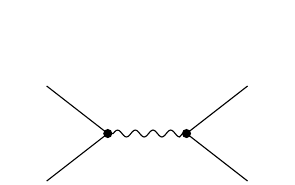
\begin{tikzpicture}[baseline = (r.base)]
      \begin{feynman}[inline = (r.base)]
        \vertex[dot] (v1) {};
        \vertex[dot] (v2) at ($ (v1) + (1,0) $) {};

        \vertex (a) at ($ (v1) + (-0.9,0.7) $) {};
        \vertex (b) at ($ (v1) + (-0.9,-0.7) $) {};
        \vertex (c) at ($ (v2) + (0.9,0.7) $) {};
        \vertex (d) at ($ (v2) + (0.9,-0.7) $) {};

        \vertex[below = 0.25em of v1] (r) {};

        \diagram* {
          (a) -- (v1) -- (b),
          (c) -- (v2) -- (d),
          (v1) -- [photon] (v2),
        };
      \end{feynman}
    \end{tikzpicture}
  \hspace{-0.4em}\Bigg|^2
  \sim \frac{\alpha^2}{T^2}
\end{equation*}
where $ \alpha \equiv g^2 / 4\pi $ is the generalized structure constant of the considered interaction. Then, dimensional analysis results into:
\begin{equation*}
  \Gamma = n \sigma v \sim T^3 \cdot \frac{\alpha^2}{T^2} \cdot 1 \sim \alpha^2 T
\end{equation*}
Now, recall \eref{eq:fried-hubble}, and in particular express it in terms of the reduced Planck mass:
\begin{equation*}
  \pl \equiv \sqrt{\frac{\hbar c}{8\pi G}} \simeq 2.4 \cdot 10^{18} \gev
  \quad \implies \quad
  H = \frac{\sqrt{\rho}}{3\pl}
\end{equation*}
The same argument as above gives $ \rho \sim T^4 $, thus $ H \sim T^2 / \pl $ and:
\begin{equation}
  \frac{\Gamma}{H} \sim \frac{\alpha^2 \pl}{T} \sim \frac{10^{16} \gev}{T}
\end{equation}
where $ \alpha \sim 0.01 $ has been used as numerical estimate. Therefore, the condition \eref{eq:thermal-eq-cond} is satisfied for $ 100 \gev \lesssim T \lesssim 10^{16} \gev $: in this range, all SM particles are in thermal equilibrium. This means that they exchange energy and momentum efficiently, thus reaching a state of maximum entropy: in this state, the number of particles per unit volume in phase space, i.e. the \emph{distribution function}, takes the form of the Bose--Einstein or the Fermi--Dirac distribution, depending on the statistics of the considered species.

On the contrary, when temperature drops below the mass of a particle species, that species becomes sub-relativistic and its distribution function acquires an exponential suppression of the form $ \sim e^{-m / T} $: this means that relativistic particles dominate the density and pressure of the primordial plasma. Furthermore, another consequence is that, had equilibrium persisted until today, the universe would be mostly photons, since any massive particle would be exponentially suppressed: this is not the case, due to the \bctxt{freeze-out} of massive particles caused by deviations from equilibrium (see \figref{fig:freeze-out} and \exref{ex:2-2-scattering}).

\begin{figure}
  \centering
  \includegraphics[width = 0.70 \textwidth]{freeze-out.png}
  \caption{Schematic illustration of freeze-out: at high temperature ($ T \gg m $) the particle abundance tracks its equilibrium value, while at low temperature ($ T \ll m $) particles freeze-out and maintain a density that is much larger than the Boltzmann-suppressed equilibrium abundance.}
  \label{fig:freeze-out}
\end{figure}

Below the scale of electroweak symmetry breaking, i.e. $ T \lesssim 100 \gev $, the gauge bosons of weak interactions receive masses through the Higgs mechanism ($ M_W \approx 80 \gev $ and $ M_Z \approx 90 \gev $), and the cross-section of weak processes becomes:
\begin{equation*}
  \sigma \sim \Bigg|\hspace{-0.4em}
    \begin{tikzpicture}[baseline = (r.base)]
      \begin{feynman}[inline = (r.base)]
        \vertex[dot] (v) {};

        \vertex (a) at ($ (v) + (-0.9,0.7) $) {};
        \vertex (b) at ($ (v) + (-0.9,-0.7) $) {};
        \vertex (c) at ($ (v) + (0.9,0.7) $) {};
        \vertex (d) at ($ (v) + (0.9,-0.7) $) {};

        \vertex[below = 0.25em of v1] (r) {};

        \diagram* {
          (a) -- (v) -- (b),
          (c) -- (v) -- (d),
        };
      \end{feynman}
    \end{tikzpicture}
  \hspace{-0.4em}\Bigg|^2
  \sim G_\text{F}^2 T^2
  \qquad \qquad
  G_\text{F} \sim \frac{\alpha}{M_W^2} \simeq 1.17 \cdot 10^{-5} \gev^{-2}
\end{equation*}
The strength of weak interactions now decreases as the temperature of the universe drops, and the ration $ \Gamma / H $ becomes:
\begin{equation}
  \frac{\Gamma}{H} \sim \frac{\alpha^2 \pl T^3}{M_W^4} \sim \left( \frac{T}{1 \mev} \right)^3
\end{equation}
The \bctxt{decoupling} of particles which interact with the primordial plasma only through weak interactions then happens at $ T_\text{dec} \sim 1 \mev $.

\newpage
\section{Equilibrium}

Observational evidence (mainly the perfect blackbody spectrum of the CMB) suggests that the early universe was in \emph{local thermal equilibrium}\footnotemark, a fact supported by the above analysis of the Standard Model at $ T \gtrsim 100 \gev $.

\footnotetext{Note that the universe can never be in perfect equilibrium, strictly speaking, since the FLRW metric does not have a time-like Killing vector. However, if the expansion is slow enough, particles have enough time to settle close to local equilibrium, and, since the universe is homogeneous, local values of thermodynamic quantities are also global values.}

\subsection{Equilibrium thermodynamics}

Consider a gas of weakly interacting particles. Quantistically, the momentum eigenstates of a particle in a volume $ V $ have a discrete spectrum: in particular, the density of states in momentum space $ \{\ve{p}\} $ is $ V / h^3 $, and the density of states in phase space $ \{\ve{x} , \ve{p}\} $ is $ 1 / h^3 $.

Considering a particle with $ g $ internal degrees of freedom (e.g. spin), in natural unit the density of states (which from now on is implicitly assumed to be in phase space) is $ g / (2\pi)^3 $. In order to obtain the number density, it is necessary to know how the particles are distributed amongst the momentum eigenstates: this information is encoded in the \emph{(phase space) distribution function} $ f(\ve{x} , \ve{p} , t) $. Homogeneity restricts $ f $ to be independent of $ \ve{x} $, while isotropy implies that the momentum-dependence is only through the magnitude $ p \equiv \norm{\ve{p}} $. The time dependence is typically left implicit, as it manifests itself in terms of the temperature dependence of the distribution function. Putting everything together, the number density of particles in real space is found to be:
\begin{equation}
  n(T) = \frac{g}{(2\pi)^3} \int \dd^3 p \, f(p,T)
  \label{eq:num-dens-def}
\end{equation}
The energy density is instead found by weighting the integration over momentum eigenstates with their energy. In particular, the assumption of the particles being weakly-interacting allows to approximate the energy as $ E(p) = \sqrt{m^2 + p^2} $, so that:
\begin{equation}
  \rho(T) = \frac{g}{(2\pi)^3} \int \dd^3 p \, f(p,T) E(p)
  \label{eq:en-dens-def}
\end{equation}
Pressure, on the other hand, requires more care.

\begin{proposition}[before upper = {\tcbtitle}]{Pressure of a weakly-interacting gas}{}
  \begin{equation}
    P = \frac{g}{(2\pi)^3} \int \dd^3 p \, f(p,T) \frac{p^2}{3E}
  \label{eq:press-def}
  \end{equation}
\end{proposition}

\begin{proofbox}
  \begin{proof}
    Consider a small area element $ \dd A $ with normal versor $ \hat{\ve{n}} $. All particles with velocity $ v \equiv \norm{\ve{v}} $, striking this area element between $ t $ and $ t + \dd t $, were located at $ t = 0 $ on a spherical shell of radius $ R = v t $ and width $ v \, \dd t $, hence a solid angle $ \dd \Omega $ of this shell defines a volume $ \dd V = R^2 v \, \dd t \dd \Omega $. Given \eref{eq:num-dens-def}, the number of particles in this volume is:
    \begin{equation*}
      \dd N = \frac{g}{(2\pi)^3} f(E,T) R^2 v \, \dd t \dd \Omega
    \end{equation*}
    Not all particles in $ \dd V $ reach the target, only those with velocities directed to the area element do. Taking into account the isotropy of the velocity distribution, the total number of these striking particles is:
    \begin{equation*}
      \dd N_A = \frac{\abs{\hat{\ve{v}} \cdot \hat{\ve{n}}} \dd A}{4 \pi R^2} \dd N = \frac{g}{(2\pi)^3} f(E,T) \frac{\abs{\hat{\ve{v}} \cdot \hat{\ve{n}}}}{4 \pi} \dd A \dd t \dd \Omega
    \end{equation*}
    where $ \hat{\ve{v}} \cdot \hat{\ve{n}} < 0 $ since the striking particles are directed towards the area element. Assuming elastic reflections, each particles transfers a momentum $ 2 \abs{\ve{p} \cdot \hat{\ve{n}}} $ to the target, hence the contribution of particles with velocity $ v $ to the pressure is:
    \begin{equation*}
      P(v) = \int \dd N_A \frac{2 \abs{\ve{p} \cdot \hat{\ve{n}}}}{\dd A \dd t} = \frac{g}{(2\pi)^3} f(E,T) \frac{p^2}{2\pi E} \int_0^{2\pi} \dd \varphi \int_{-1}^0 \dd \cos \theta \, \cos^2 \theta = \frac{g}{(2\pi)^3} f(E,T) \frac{p^2}{3E}
    \end{equation*}
    where $ v = p / E $ was used, and $ \theta $ was defined as $ \hat{\ve{v}} \cdot \hat{\ve{n}} = - \cos \theta < 0 $. Integrating over energy or momentum yields the thesis.
  \end{proof}
\end{proofbox}

The form of the distribution function depends on the thermodynamical state of the system. Assuming that the gas is in \emph{kinetic equilibrium}, i.e. if the particles can exchange energy and momentum efficiently, then the system is in a state of maximal entropy and the distribution function is either the Fermi--Dirac distribution (fermions) or the Bose--Einstein distribution (bosons):
\begin{equation}
  f(p,T) = \left[ e^\frac{E(p) - \mu(T)}{T} \pm 1 \right]^{-1}
\end{equation}
with the $ + $ sign for fermions and the $ - $ sign for bosons. At low temperatures, i.e. $ T < E - \mu $, both distributions reduce to the Maxwell--Boltzmann distribution:
\begin{equation}
  f(p,T) \approx e^{- \frac{E(p) - \mu(T)}{T}}
\end{equation}
The chemical potential $ \mu(T) $ characterizes the response of a system to a change in particle number: the second law of thermodynamics implies that, given a reaction, particles flow towards the side of the reaction with the lower total chemical potential, until \emph{chemical equilibrium} is achieved:
\begin{equation*}
  \sum_\text{reactants} \mu_i = \sum_\text{products} \mu_j
\end{equation*}
Note that, since the number of photons is not conserved (e.g. double Compton scattering $ e^- \gamma \lra e^- \gamma \gamma $), then $ \mu_\gamma = 0 $ and $ \mu_{\bar{X}} = - \mu_X $, due to particle-antiparticle annihilation $ X \bar{X} \lra \gamma \gamma $.

A system is in \bctxt{thermal equilibrium} if its species are both in kinetic and chemical equilibrium: these species then share a common temperature $ T_i = T $, which is often identified with the photon temperature $ T_\gamma $ (the ``temperature of the universe").

\subsection{Density and pressure}

At early times, the chemical potentials of all particles are so small that they can be neglected, thus \eeref{eq:num-dens-def}{eq:en-dens-def} can be written as:
\begin{equation}
  n(T) = \frac{g}{2\pi^2} T^3 I_\pm(x)
  \qquad \qquad
  \rho(T) = \frac{g}{2\pi^2} T^4 J_\pm(x)
  \label{eq:exact-rho}
\end{equation}
with $ x \equiv m / T $, $ \xi \equiv p / T $ and:
\begin{equation}
  I_\pm(x) \equiv \int_0^\infty \dd \xi \frac{\xi^2}{\exp \sqrt{\xi^2 + x^2} \pm 1}
  \qquad \qquad
  J_\pm(x) \equiv \int_0^\infty \dd \xi \frac{\xi^2 \sqrt{\xi^2 + x^2}}{\exp \sqrt{\xi^2 + x^2} \pm 1}
  \label{eq:integrals}
\end{equation}
These integrals need, in general, to be evaluated numerically, but analytic expressions are possible in the ultra-relativistic and sub-relativistic limits.

\begin{lemma}{Ultra-relativistic limit}{}
  In the limit of $ T \gg m $, i.e. $ x \ra 0 $:
  \begin{equation}
    n(T) = \frac{\zeta(3)}{\pi^2} g T^3
    \begin{cases}
      1 & \text{bosons} \\
      \tfrac{3}{4} & \text{fermions}
    \end{cases}
    \qquad \qquad
    \rho(T) = \frac{\pi^2}{30} g T^4
    \begin{cases}
      1 & \text{bosons} \\
      \tfrac{7}{8} & \text{fermions} \\
    \end{cases}
    \label{eq:ultra-rel}
  \end{equation}
\end{lemma}

\begin{proofbox}
  \begin{proof}
    For $ x \ra 0 $, the integrals in \eref{eq:integrals} reduce to:
    \begin{equation*}
      I_\pm(0) = \int_0^\infty \dd \xi \frac{\xi^2}{e^\xi \pm 1}
      \qquad \qquad
      J_\pm(0) = \int_0^\infty \dd \xi \frac{\xi^3}{e^\xi \pm 1}
    \end{equation*}
    These integrals can be solved using the standard integral:
    \begin{equation}
      \int_0^\infty \dd \xi \frac{\xi^n}{e^\xi - 1} = \zeta(n + 1) \Gamma(n + 1)
    \end{equation}
    In the bosonic case they are straightforward: $ I_-(0) = 2 \zeta(3) $ and $ J_-(0) = 6 \zeta(4) = \frac{\pi^4}{15} $. In the fermionic case, use instead:
    \begin{equation*}
      \frac{1}{e^\xi + 1} = \frac{1}{e^\xi - 1} - \frac{2}{e^{2\xi} - 1}
    \end{equation*}
    so that:
    \begin{equation*}
      I_+(0) = I_-(0) - 2 \left( \frac{1}{2} \right)^3 I_-(0) = \frac{3}{2} I_-(0)
    \end{equation*}
    \begin{equation*}
      J_+(0) = J_-(0) - 2 \left( \frac{1}{2} \right)^4 J_-(0) = \frac{7}{8} J_-(0)
    \end{equation*}
    which concludes the proof.
  \end{proof}
\end{proofbox}

From \eref{eq:press-def} with $ E \simeq p $ in the relativistic limit, the equation of state for a relativistic gas $ P = \frac{1}{3} \rho $ is recovered. Moreover, recalling \eref{eq:omega-def}, using $ T_0 = 2.73 \,\text{K} $ it is possible to compute the density parameter of radiation:
\begin{equation*}
  \rho_{\gamma,0} = \frac{\pi^2}{15} T_0^4 \simeq 4.6 \cdot 10^{-34} \,\text{g} \,\text{cm}^{-3}
  \quad \implies \quad
  \Omega_\gamma h^2 \simeq 2.5 \cdot 10^{-5}
\end{equation*}

\begin{lemma}{Sub-relativistic limit}{}
  In the limit $ T \ll m $, i.e. $ x \gg 1 $:
  \begin{equation}
    n(T) = g \left( \frac{m T}{2\pi} \right)^{3/2} e^{-m/T}
    \qquad \qquad
    \rho(T) = m n(T) + \frac{3}{2} n(T) T
    \label{eq:sub-rel}
  \end{equation}
\end{lemma}

\begin{proofbox}
  \begin{proof}
    For $ x \gg 1 $:
    \begin{equation*}
      I_\pm(x) \approx \int_0^\infty \dd \xi \, \xi^2 e^{-\sqrt{\xi^2 + x^2}}
    \end{equation*}
    Most of the contribution comes from the $ \xi \ll x $ regime, hence, at lowest order in $ \xi $:
    \begin{equation*}
      I_\pm(x) \approx \int_0^\infty \dd \xi \, \xi^2 \exp \left( x + \frac{\xi^2}{2x} \right) = (2x)^{3/2} e^{-x} \int_0^\infty \dd \xi \, \xi^2 e^{-\xi^2}
    \end{equation*}
    Recalling the standard integral:
    \begin{equation}
      \int_0^\infty \dd \xi \, \xi^n e^{-\xi^2} = \frac{1}{2} \Gamma\left( \frac{n + 1}{2} \right)
    \end{equation}
    with $ \Gamma(\frac{3}{2}) = \frac{\sqrt{\pi}}{2} $:
    \begin{equation*}
      I_\pm(x) = \sqrt{\frac{\pi}{2}} x^{3/2} e^{-x}
      \quad \implies \quad
      n(T) = g \left( \frac{m T}{2\pi} \right)^{3/2} e^{-m/T}
    \end{equation*}
    For the energy density, use the sub-relativistic expansion at lowest order in $ \xi $ in \eref{eq:integrals}:
    \begin{equation*}
      \begin{split}
        J_\pm(x)
        & \approx \int_0^\infty \dd \xi \, \xi^2 \left( x + \frac{\xi^2}{2x} \right) \exp \left( x + \frac{\xi^2}{2x} \right) = (2x)^{3/2} e^{-x} \int_0^\infty \dd \xi \, \xi^2 \left( x + \xi^2 \right) e^{-\xi^2} \\
        & = (2x)^{3/2} e^{-x} \frac{1}{2} \left[ x \Gamma \left( \frac{3}{2} \right) + \Gamma \left( \frac{5}{2} \right) \right] = \sqrt{\frac{\pi}{2}} x^{3/2} e^{-x} \left( x + \frac{3}{2} \right)
      \end{split}
    \end{equation*}
    Inserting $ x = m / T $ yields the thesis.
  \end{proof}
\end{proofbox}

In a similar way, from \eref{eq:press-def} it can be shown that $ P = n T $, which means that a non-relativistic gas behaves like pressureless dust since $ P = n T \ll n m = \rho $.

As expected, in the sub-relativistic limit $ T \ll m $ the number density, the energy density and the pressure of massive particle species fall exponentially (Boltzmann suppression). This is interpreted as the annihilation of particles with antiparticles: at high temperature (i.e. energy), matter-antimatter annihilation is balanced by pair production, but as $ T $ decreases below the mass of the particle the thermal energy is no longer sufficient for pair production and the number density decreases exponentially.

\subsection{Effective number of relativistic species}

From now on, the temperature of the universe is identified with the temperature of the photon gas: $ T \equiv T_\gamma $.

\begin{definition}{Effective number of relativistic degrees of freedom}{}
  The total radiation density in the universe is defined as:
  \begin{equation}
    \rho_\text{r} \defeq \sum_i \rho_i \equiv \frac{\pi^2}{30} \dof(T) T^4
    \label{eq:rad-en-dens-def}
  \end{equation}
  where the sum runs over all relativistic particle species. The \bcdef{effective number of relativistic degrees of freedom} is denoted by $ \dof(T) $.
\end{definition}

Note that $ \dof(T) $ receives different contributions from relativistic species in thermal equilibrium with the photons, i.e. with $ T = T_i \gg m_i $, and from decoupled relativistic species, i.e. with $ T \neq T_i \gg m_i $. In particular, from \eref{eq:ultra-rel}:
\begin{equation}
  \dof^\text{eq}(T) = \sum_\text{bosons} g_i + \frac{7}{8} \sum_\text{fermions} g_j
  \qquad \quad
  \dof^\text{dec}(T) = \sum_\text{bosons} g_i \left( \frac{T_i}{T} \right)^4 + \frac{7}{8} \sum_\text{fermions} g_j \left( \frac{T_j}{T} \right)^4
\end{equation}
When the temperature drops below the mass $ m_i $ of a particle species, it becomes non-relativistic and no longer contributes to $ \dof(T) $.

\begin{example}{$ \dof(T) $ above $ 100 \gev $}{}
  For $ T \gtrsim 100 \gev $, all SM particles are relativistic (as noted in \secref{sec:hot-big-bang}), hence all species contribute to $ \dof^\text{eq}(T) $. The bosons have:
  \begin{equation*}
    g_\text{b} = g_\gamma + g_g + g_{W,Z} + g_H = 2_\text{spin} + 8_\text{colour} \cdot 2_\text{spin} + 3_{\SUn{2}} \cdot 3_\text{spin} + 1_\text{spin} = 28
  \end{equation*}
  since massless vector bosons only have transverse polarization. The fermions, on the other hand, have:
  \begin{equation*}
    \begin{split}
      g_\text{f}
      & = g_q + g_{e,\mu,\tau} + g_\nu \\
      & = 6_\text{species} \cdot 2_\text{spin} \cdot 2_\text{anti} \cdot 3_\text{colour} + 3_\text{species} \cdot 2_\text{spin} \cdot 2_\text{anti} + 3_\text{species} \cdot 1_\text{spin} \cdot 2_\text{anti} = 90
    \end{split}
  \end{equation*}
  since neutrinos only have one helicity state (left-handed neutrinos and right-handed antineutrinos). The effective number of relativistic degrees of freedom then is:
  \begin{equation}
    \dof = g_\text{b} + \tfrac{7}{8} g_\text{f} = 106.75
  \end{equation}
  As the temperature drops, various particle species become non-relativistic and annihilate: the evolution of $ \dof(T) $ is plotted in \figref{fig:rel-dof}. At $ T \sim 150 \mev $, before the strange quarks have time to annihilate, the QCD phase transition takes place: quarks combine into baryons and mesons, which are all non-relativistic under $ 150 \mev $, except for the pions ($ \pi^\pm , \pi^0 $). The only relativistic species left are then pions, electrons, muons, neutrinos and photons: since the pions are spin-$ 0 $ particles, they contribute to $ g_\text{b} $ with $ g_\pi = 3_\text{species} \cdot 1_\text{spin} $, resulting in $ \dof = 2 + 3 + \frac{7}{8} \cdot (4 + 4 + 6) = 17.25 $.

  Moreover, it is important to note that the transition from relativistic to non-relativistic behaviour is not instantaneous: about $ 80\% $ of the particle-antiparticle annihilations takes place in the interval $ T = m \ra T = \frac{1}{6} m $.
\end{example}

\begin{figure}
  \centering
  \includegraphics[width = 0.8 \textwidth]{rel-dof.png}
  \caption{Evolution of $ \dof(T) $ with temperature, assuming Standard Model particles. The dotted line is the effective number of degrees of freedom in entropy $ \dofs(T) $.}
  \label{fig:rel-dof}
\end{figure}

\subsubsection{Entropy}

According to the second law of thermodynamics, the total entropy of the universe can only increase or stay constant. Since the fraction of baryons to photons is measured to be:
\begin{equation}
  \eta_\text{b} \equiv \frac{n_\text{b}}{n_\gamma} \simeq 5.5 \cdot 10^{-10} \frac{\Omega_\text{b} h^2}{0.020} \sim 10^{-9}
\end{equation}
the entropy of the universe is dominated by the entropy of the photon bath (at least as long as the universe is sufficiently uniform): any entropy production from non-equilibrium processes is then insignificant relative to the total entropy, and therefore the expansion of the universe can be treated as \emph{adiabatic}, so that the total entropy stays constant, even beyond equilibrium.

\begin{lemma}{Entropy at equilibrium}{}
  The entropy of a system at equilibrium stays constant.
\end{lemma}

\begin{proofbox}
  \begin{proof}
    Consider the second law of thermodynamics: $ T \dd S = \dd U + P \dd V $. Using $ U = \rho V $:
    \begin{equation*}
      \dd S = \frac{\dd [(\rho + P) V]}{T} - \frac{V \dd P}{T} = \frac{V}{T} \frac{\pa \rho}{\pa T} \dd T + \frac{\rho + P}{T} \dd V
    \end{equation*}
    Since the entropy function must exist, this differential form must be exact. By \tref{th:poincare}, an exact form is also closed, hence:
    \begin{equation}
      \frac{\pa}{\pa V} \left[ \frac{V}{T} \frac{\pa \rho}{\pa T} \right] = \frac{\pa}{\pa T} \left[ \frac{\rho + P}{T} \right]
      \quad \implies \quad
      \frac{\pa P}{\pa T} = \frac{\rho + P}{T}
      \label{eq:pt-thermo}
    \end{equation}
    Rearranging the second law of thermodynamics, then:
    \begin{equation*}
      \dd S = \frac{\dd [(\rho + P) V]}{T} - \frac{(\rho + P) V}{T^2} \dd T = \dd \left[ \frac{\rho + P}{T} V \right]
    \end{equation*}
    Tho show that entropy is conserved in equilibtrium, consider:
    \begin{equation*}
      \begin{split}
        \frac{\dd S}{\dd t} = \frac{\dd}{\dd t} \left[ \frac{\rho + P}{T} V \right] = \frac{V}{T} \left[ \dot{\rho} + \frac{\dot{V}}{V} (\rho + P) \right] + \frac{V}{T} \left[ \dot{P} - \frac{\rho + P}{T} \dot{T} \right]
      \end{split}
    \end{equation*}
    Since $ V \propto a^3 $, then $ \dot{V} / V = 3H $ and the first term vanishes by \eref{eq:r-p}, while the second vanishes by \eref{eq:pt-thermo}. Therefore, $ \dot{S} = 0 $ at equilibrium.
  \end{proof}
\end{proofbox}

It is convenient to define the \bctxt{entropy density}, which ignoring a constant integration constant is (by the above proof):
\begin{equation}
  s = \frac{\rho + P}{T}
\end{equation}
which, by adiabaticity (i.e. $ \dd Q = 0 \, \implies \, \dd S = 0 $), scales like $ s \propto a^{-3} $. Since for a relativistic gas $ P = \frac{1}{3} \rho $, recalling \eref{eq:ultra-rel} it is possible to express the entropy density in the ultra-relativistic limit as:
\begin{equation}
  s = \frac{2\pi^2}{45} g(T) T^3
\end{equation}

\begin{definition}{Effective number of relativistic degrees of freedom in entropy}{}
  The total entropy density in the universe is defined as:
  \begin{equation}
    s \defeq \sum_i s_i \equiv \frac{2\pi^2}{45} \dofs(T) T^3
    \label{eq:s-def}
  \end{equation}
  where the sum runs over all relativistic particle species. The \bcdef{effective number of degrees of freedom in entropy} is denoted by $ \dofs(T) $.
\end{definition}

As for $ \dof(T) $, there are two different contributions to $ \dofs(T) $ too: one from species in thermal equilibrium with the photon bath and one from decoupled species. Note that $ \dofs^\text{eq}(T) = \dof^\text{eq}(T) $, while, since $ s_i \propto T_i^3 $, for decoupled species:
\begin{equation}
  \dofs^\text{dec}(T) = \sum_\text{bosons} g_i \left( \frac{T_i}{T} \right)^3 + \frac{7}{8} \sum_\text{fermions} g_j \left( \frac{T_j}{T} \right)^3
\end{equation}
which is $ \dofs^\text{dec}(T) \neq \dof^\text{dec}(T) $. It follows that $ \dof(T) = \dofs(T) $ only when \emph{all} relativistic species are in thermal equilibrium with the photon bath: in the real universe, this is the case for until $ t \approx 1 \,\text{sec} $ (see \figref{fig:rel-dof}).
The conservation of entropy has two important consequences:
\begin{itemize}
  \item since $ s \propto a^{-3} $, if the number of particles in a comoving volume $ N_i $ is conserved (i.e. $ n_i \propto a^{-3} $), then $ n_i \propto s $, with $ N_i = n_i / s $ since it is a scale-invariant quantity. This is the case, for example, for the net baryon number after baryogenesis, which is conserved, hence $ N_\text{net} \equiv (n_\text{B} - n_{\bar{\text{B}}}) / s $ is constant;
  \item from the definition of $ s $, it follows that $ T \propto \dofs^{-1/3} a^{-1} $. Away from mass thresholds, $ \dofs $ is approximately constant and $ T \propto a^{-1} $ as expected, but when a particle species becomes non-relativistic the factor $ \dofs $ accounts for the transfer of its entropy to other relativistic species, making $ T $ change in the scaling as a consequence.
\end{itemize}

\subsubsection{Neutrino decoupling}

Neutrinos are coupled to the thermal bath only through weak interaction processes (e.g. $ \nu_e \bar{\nu}_e \lra e^+ e^- $), whose cross-section is estimated as $ \sigma \sim G_\text{F}^2 T^2 $. By \eref{eq:int-rate-def}, then, $ \Gamma \sim G_\text{F}^2 T^5 $, which allows to estimate the temperature for neutrino decoupling (with $ H \sim T^2 / \pl $):
\begin{equation*}
  \frac{\Gamma}{H} \sim \left( \frac{T}{1 \mev} \right)^3
  \quad \implies \quad
  T_\text{dec} \sim 1 \mev
\end{equation*}
A more accurate computation gives $ T_\text{dec} \sim 0.8 \mev $. After decoupling, neutrinos move freely along geodesics. Since $ p \propto a^{-1} $ (by \eref{eq:geodesic-momentum}), it is convenient to define the time-independent combination $ q \equiv a p $, so that the neutrino number density after decoupling can be written as:
\begin{equation*}
  n_\nu \propto a^{-3} \int \dd^3 q \left[ \exp \frac{q}{a T_\nu} + 1 \right]^{-1}
\end{equation*}
But, after decoupling, particle number conservation requires $ n_\nu \propto a^{-3} $, hence the neutrino temperature must scale as $ T_\nu \propto a^{-1} $. The neutrinos then follow a relativistic Fermi--Dirac distribution with decreasing temperature, even after they become non-relativistic at later times (when $ T_\nu \ll m_\mu $), due to the Louville theorem\footnotemark.

\footnotetext{The Liouville theorem states that, in a Hamiltonian system, the phase-space probability density (i.e. distribution function) is constant along the trajectories defined by the Hamilton equations of motion.}

\subsubsection{Electron-positron annihilation}

Shortly after the neutrinos decouple, the temperature drops below the electron mass ($ m_e \simeq 0.511 \mev $), so that electron-positron annihilation is no longer balanced by the $ \gamma \gamma \ra e^- e^+ $ pair production. The energy density and entropy of electrons and positrons are then transferred to the photons, but not to the decoupled neutrinos: the photons are thus heated relative to the neutrinos (see \figref{fig:neutrino-temp}).

\begin{figure}
  \centering
  \includegraphics[width = 0.70 \textwidth]{neutrino-temp.png}
  \caption{Difference in redshift between neutrino temperature $ T_\nu \propto a^{-1} $ and photon temperature $ T_\gamma \propto \dofs^{-1/3} a^{-1} $.}
    \label{fig:neutrino-temp}
\end{figure}

To quantify this effect, consider the change in the effective number of degrees of freedom in entropy. Neglecting neutrinos and other decoupled species\footnotemark:
\begin{equation*}
  \dofs^\text{eq} =
  \begin{cases}
    2_\gamma + \frac{7}{8} \cdot 4_e = \frac{11}{2} & T \gtrsim m_e \\
    2_\gamma = 2 & T < m_e
  \end{cases}
\end{equation*}

\footnotetext{Entropy is conserved separately for the thermal bath and the decoupled species, since they are non-interacting systems.}

Since, in equilibrium, $ \dofs^\text{eq} T^3 a^3 $ remains constant, the photon temperature $ a T_\gamma \equiv a T $ must increase by a factor of $ (11/4)^{1/3} $ after electron-positron annihilation, while $ a T_\nu $ remains the same. This means that, for $ T < m_e $:
\begin{equation}
  T_\nu = \sqrt[3]{\frac{4}{11}} T_\gamma
  \label{eq:t-nu-gamma}
\end{equation}
For $ T \ll m_e $, the only remaining relativistic species are photons and neutrinos, and the above equation implies that $ \dof \neq \dofs $:
\begin{equation*}
  \dof = 2_\gamma + \frac{7}{8} \cdot 2_\text{anti} \cdot N_\text{eff} \left( \frac{4}{11} \right)^{4/3} = 3.36
  \qquad \qquad
  \dofs = 2_\gamma + \frac{7}{8} \cdot 2_\text{anti} \cdot N_\text{eff} \left( \frac{4}{11} \right) = 3.94
\end{equation*}
where $ N_\text{eff} $ is the \bctxt{effective number of neutrino species}. If neutrino decoupling was instantaneous, then $ N_\text{eff} = 3 $; however, neutrino decoupling was not complete when $ e^+ e^- $ annihilation began, so a fraction of the released energy and entropy did leak to the neutrinos, resulting into $ N_\text{eff} = 3.046 $ (the current bound from the Planck satellite is $ N_\text{eff} = 3.04 \pm 0.18 $).

Note that \eref{eq:t-nu-gamma} holds until the present, thus allowing to estimate the temperature of the \bctxt{cosmic neutrino background} (C$ \nu $B): given the present CMB temperature $ T_\text{CMB} = 2.73 \,\text{K} = 0.24 \mmev $, it is $ T_\text{C$ \nu $B} = 1.95 \,\text{K} = 0.17 \mmev $. From \eref{eq:ultra-rel}, the number density of neutrinos is:
\begin{equation}
  n_\nu = \frac{3}{4} N_\text{eff} \cdot \frac{4}{11} n_\gamma
\end{equation}
which today corresponds to $ n_\nu / N_\text{eff} \simeq 112 \,\text{cm}^{-3} $ per flavour, as $ n_\gamma(2.73 \,\text{K}) \simeq 5 \,\text{K}^3 \simeq 415 \,\text{cm}^{-3} $. On the other hand, the present energy density of neutrinos depends on whether they are relativistic or non-relativistic today:
\begin{itemize}
  \item massless neutrinos: massless neutrinos are always relativistic, hence, by \eref{eq:ultra-rel}:
    \begin{equation*}
      \rho_\nu = \frac{7}{8} N_\text{eff} \left( \frac{4}{11} \right)^{4/3} \rho_\gamma \quad \implies \quad \Omega_\nu h^2 \simeq 1.7 \cdot 10^{-5}
    \end{equation*}
    were $ \Omega_\gamma h^2 \simeq 2.5 \cdot 10^{-5} $ was used;
  \item massive neutrinos: experiments on neutrino oscillations impose constraints on the sum of neutrino masses: $ 60 \mmev < \sum_i m_{\nu_i} < 1 \ev $. This means that neutrinos behave as radiation-like particles in the early universe ($ T \gg m_\nu $) and as matter-like particles in the late universe ($ T \ll m_\nu $), which means that $ \rho_{\nu,0} \approx \sum_i m_{\nu_i} n_{\nu_i , 0} $ (by \eref{eq:sub-rel}). Using the estimate $ n_{\nu_i} \simeq 112 \,\text{cm}^{-3} $:
    \begin{equation}
      \Omega_\nu h^2 \approx \frac{\sum_i m_{\nu_i}}{95 \ev}
    \end{equation}
    Hence neutrinos are a subdominant component, with $ 0.001 \lesssim \Omega_\nu \lesssim 0.02 $ (using $ h = 0.7 $).
\end{itemize}

\subsection{Thermal history}

In radiation era $ a \propto \sqrt{t} $, hence $ H = \frac{1}{2t} $ and, using \eref{eq:rad-en-dens-def}:
\begin{equation}
  \frac{1}{2t} = H \simeq \sqrt{\frac{\rho_\text{r}}{3\pl^2}} \simeq \frac{\pi}{3} \sqrt{\frac{\dof}{10}} \frac{T^2}{\pl}
  \quad \implies \quad
  \frac{T}{1 \mev} \simeq 1.5 \dof^{-1/4} \sqrt{\frac{1 \,\text{sec}}{t}}
  \label{eq:thermal-history}
\end{equation}
Therefore, $ 1 $ second after the Big Bang the universe was about $ 1 \mev $. It is also possible to state an approximated thermal history of the universe (recalling \eref{eq:redshift-a}):

\begin{center}
  \begin{tabular}{cccc}
    \hline
    \hspace{5em} Event \hspace{5em} & \hspace{1em} time $ t $ \hspace{1em} & \hspace{1em} redshift $ z $ \hspace{1em} & \hspace{1em} temperature $ T $ \hspace{1em} \\
    \hline
    \textbf{Singularity} & $ \ve{0} $ & $ \bs{\infty} $ & $ \bs{\infty} $ \\ [1ex]
    Inflation & $ \sim 10^{-35} \,\text{s} $ & $ \sim 10^{28} $ & $ \sim 10^{15} \gev $ \\ [1ex]
    Baryogenesis & $ \lesssim 20 \,\text{ps} $ & $ > 10^{15} $ & $ > 100 \gev $ \\ [1ex]
    EW phase transition & $ 20 \,\text{ps} $ & $ 10^{15} $ & $ 100 \gev $ \\ [1ex]
    QCD phase transition & $ 20 \,\mu\text{s} $ & $ 10^{12} $ & $ 150 \mev $ \\ [1ex]
    Dark matter freeze-out & ? & ? & ? \\ [1ex]
    Neutrino decoupling & $ 1 \,\text{s} $ & $ 6 \cdot 10^9 $ & $ 1.5 \mev $ \\ [1ex]
    $ e^- e^+ $ annihilation & $ 6 \,\text{s} $ & $ 2 \cdot 10^9 $ & $ 500 \kev $ \\ [1ex]
    Big Bang nucleosynthesis & $ 3 \,\text{min} $ & $ 4 \cdot 10^8 $ & $ 100 \kev $ \\ [1ex]
    Matter-radiation equality & $ 60 \,\text{kyr} $ & $ 3400 $ & $ 0.75 \ev $ \\ [1ex]
    Recombination & $ 260 - 380 \,\text{kyr} $ & $ 1100 - 1400 $ & $ 0.26 - 0.33 \ev $ \\ [1ex]
    Photon decoupling (CMB) & $ 380 \,\text{kyr} $ & $ 1100 $ & $ 0.26 \ev $ \\ [1ex]
    Reionization & $ 100 - 400 \,\text{Myr} $ & $ 10 - 30 $ & $ 2.6 - 7.0 \mmev $ \\ [1ex]
    $ \Lambda $-matter equality & $ 9 \,\text{Gyr} $ & $ 0.4 $ & $ 0.33 \mmev $ \\ [1ex]
    \textbf{Today} & $ \ve{13.8} \, \text{\textbf{Gyr}} $ & $ \ve{0} $ & $ \ve{0.24} \, \text{\textbf{meV}} $ \\
    \hline
  \end{tabular}
\end{center}

Note that the expansion of the universe during Inflation had a very different timescale with respect to today, although in both cases it is exponential ($ a \propto \exp H t $):
\begin{equation*}
  H_\text{I} \sim \frac{T_\text{I}^2}{\pl} \sim 10^{11} \gev
  \quad \implies \quad
  t_{H_\text{I}} \equiv \frac{1}{H_\text{I}} \sim 10^{-35} \,\text{sec}
\end{equation*}
\begin{equation*}
  H_0 \approx \frac{70 \,\text{km} \,\text{s}^{-1}}{1 \,\text{Mpc}}
  \quad \implies \quad
  t_{H_0} \equiv \frac{1}{H_0} \sim 4.5 \cdot 10^{17} \,\text{sec}
\end{equation*}
The expansion during Inflation was $ \sim 10^{52} $ times faster than it is today.

\newpage
\section{Beyond equilibrium}

\subsection{Boltzmann equation}

In the absence of interactions, the number of particles in a fixed physical volume $ V \propto a^3 $ is conserved, thus $ n_i \propto a^{-3} $ and:
\begin{equation*}
  \frac{\dot{n}_i}{n_i} = - 3 \frac{\dot{a}}{a}
  \quad \iff \quad
  \frac{1}{a^3} \frac{\dd (n_i a^3)}{\dd t} = 0
\end{equation*}
To include the effect of interactions, a collision term $ C_i(\{n_j\}) $ is added, which depends on the number density of all particle species:
\begin{equation}
  \frac{1}{a^3} \frac{\dd (n_i a^3)}{\dd t} = C_i(\{n_j\})
\end{equation}
This is the \bctxt{Boltzmann equation}, which describes the behaviour of the system beyond equilibrium. The form of the collision term depends on the specific interactions under consideration: interactions between three or more particles are very unlikely, so it is reasonable to assume only single-particle decays and two-particle scatterings/annihilations.

\begin{example}{$ 2 \lra 2 $ scattering}{2-2-scattering}
  Consider a generic process $ 1 + 2 \lra 3 + 4 $, and suppose to track the number density $ n_1 $ of species $ 1 $. The rate of change in the abundance of species $ 1 $ is given by the difference between the rates of annihilation (direct process) and production (inverse process) of the species, hence:
  \begin{equation*}
    \frac{1}{a^3} \frac{\dd (n_1 a^3)}{\dd t} = - \alpha n_1 n_2 + \beta n_3 n_4
  \end{equation*}
  The first term describes the direct process, and the parameter $ \alpha = \braket{\sigma v} $ is the \emph{thermally-averaged cross-section}\footnote{The angle brackets denote an average over the relative velocity $ v $ between particles $ 1 $ and $ 2 $.}. To determine the parameter $ \beta $, note that the collision term must vanish at (chemical) equilibrium, so that:
  \begin{equation*}
    \beta = \left( \frac{n_1 n_2}{n_3 n_4} \right)_\text{eq} \alpha
  \end{equation*}
  where the equilibrium number densities are given by \eref{eq:num-dens-def}. The Boltzmann equation then becomes:
  \begin{equation}
    \frac{1}{a^3} \frac{\dd (n_1 a^3)}{\dd t} = - \braket{\sigma v} \left[ n_1 n_2 - \left( \frac{n_1 n_2}{n_3 n_4} \right)_\text{eq} n_3 n_4 \right]
    \label{eq:boltzmann-2-2}
  \end{equation}
  Rewriting this equation in terms of the number of particles in a comoving volume $ N_i \equiv n_i / s $:
  \begin{equation}
    \frac{\dd \ln N_1}{\dd \ln a} = - \frac{\Gamma_1}{H} \left[ 1 - \left( \frac{N_1 N_2}{N_3 N_4} \right)_\text{eq} \frac{N_3 N_4}{N_1 N_2} \right]
  \end{equation}
  with the interaction rate $ \Gamma_1 \equiv n_2 \braket{\sigma v} $. The r.h.s. contains two different factors: the $ \Gamma_1 / H $ factor, describing the \bcex{interaction efficiency}, and the $ [1 - \dots] $ factor, describing the \bcex{deviation from equilibrium}. There are two main regimes for the reaction:
  \begin{itemize}
    \item $ \Gamma_1 \gg H $: the natural state of the system is chemical equilibrium since, given the large interaction rate, if $ N_1 \gg N_1^\text{eq} $ the r.h.s. is negative and $ N_1 $ reduces towards $ N_1^\text{eq} $, while if $ N_1 \ll N_1^\text{eq} $ the r.h.s. is positive and $ N_1 $ increases towards $ N_1^\text{eq} $. At equilibrium, then, the r.h.s. vanishes and particles assume their equilibrium abundances;
    \item $ \Gamma_1 < H $: when the reaction rate drops below the Hubble scale, the r.h.s. gets suppressed and the comoving density of particles approaches a constant \emph{relic density}, a phenomenon known as \bcex{freeze-out}.
  \end{itemize}
\end{example}

\subsection{Dark matter relics}

In this section, the hypothesis that dark matter is composed of weakly interacting massive particles (WIMPs) is assumed. WIMPs were in close contact with the rest of the cosmic plasma at high temperatures, but then experiences freeze-out at a critical temperature $ T_\text{f} $, which can be estimated using the Boltzmann equation.

\subsubsection{Dark matter freeze-out}

Some assumptions on the WIMP interactions have to be made. In particular, assume that a heavy dark matter particle $ X $ and its antiparticle $ \bar{X} $ can annihilate to produce two light (essentially massless) particle:
\begin{equation*}
  X + \bar{X} \lra \ell + \bar{\ell}
\end{equation*}
Moreover, assume the light particles to be tightly coupled to the cosmic plasma (e.g. if they are charged), so that they maintain their equilibrium densities $ n_\ell = n_\ell^\text{eq} $, and also that there are no initial asymmetries between $ X $ and $ \bar{X} $, i.e. $ n_X = n_{\bar{X}} $. \eref{eq:boltzmann-2-2} for the number of WIMPs in a comoving volume $ N_X \equiv n_X / s $ then is:
\begin{equation*}
  \frac{\dd N_X}{\dd t} = - s \braket{\sigma v} [N_X^2 - (N_X^\text{eq})^2]
\end{equation*}
Since the interesting dynamics takes place at $ T \sim M_X $, define $ x \equiv M_X / T $, so that:
\begin{equation*}
  \frac{\dd x}{\dd t} = \frac{\dd}{\dd t} \frac{M_X}{T} = - \frac{1}{T} \frac{\dd T}{\dd t} x \simeq H x
\end{equation*}
where $ T \propto a^{-1} $ was used (assuming $ \dofs \simeq \text{const.} \equiv \dofs(M_X) $) for the times relevant to freeze-out. Assuming radiation domination\footnotemark, i.e. $ H = H(M_X) / x^2 $, the Boltzmann equation reduces to the so-called \bctxt{Riccati equation}:
\begin{equation}
  \frac{\dd N_X}{\dd x} = - \frac{\lambda}{x^2} [N_X^2 - (N_X^\text{eq})^2]
\end{equation}
with:
\begin{equation}
  \lambda \equiv \frac{2\pi^2}{45} \dofs \frac{M_X^3 \braket{\sigma v}}{H(M_X)}
\end{equation}

\footnotetext{From \eref{eq:thermal-history} (with $ \dof \simeq \text{const.} $) $ H / T^2 = \text{const.} $, hence $ H / T^2 = H(M_X) / M_X^2 $, i.e. $ H = H(M_X) / x^2 $.}

This parameter can be treated as a constant in most WIMP theories, but, despite this, the Riccati equation has no analytic solutions. Numerical solutions for two different values of $ \lambda $ are pictured in \figref{fig:dm-freeze}: at high temperatures ($ x < 1 $) $ N_X \approx N_X^\text{eq} \simeq 1 $, while at low temperatures ($ x \gg 1 $) the equilibrium abundance is exponentially suppressed as $ N_X^\text{eq} \sim e^{-x} $. Ultimately, WIMPs will become so rare that they will not be able to find each other fast enough to maintain the equilibrium abundance: numerically, this freeze-out happens at $ x_\text{f} \sim 10 $, where the solution $ N_X $ to the Riccati equation starts to deviate significantly from the Boltzmann-suppressed equilibrium abundance $ N_X^\text{eq} $.

\begin{figure}
  \centering
  \includegraphics[width = 0.7 \textwidth]{dm-freeze.png}
  \caption{Abundance of WIMPs as the temperature drops below their mass.}
  \label{fig:dm-freeze}
\end{figure}

The final relic abundance $ N_X^\infty \equiv N_X(x = \infty) $ determines the freeze-out density of dark matter, and it can be estimated as a function of $ \lambda $. For $ x \gg x_\text{f} $ (after freeze-out), $ N_X $ will be much larger than $ N_X^\text{eq} $, hence the Riccati equation reduces to:
\begin{equation*}
  \frac{\dd N_X}{\dd x} \simeq - \frac{\lambda}{x^2} N_X^2
\end{equation*}
Integrating over the domain $ (x_\text{f} , \infty) $, the following solution is found:
\begin{equation*}
  \frac{1}{N_X^\infty} - \frac{1}{N_X^\text{f}} = \frac{\lambda}{x_\text{f}}
\end{equation*}
with $ N_X^\text{f} \equiv N_X(x_\text{f}) $. Typically $ N_X^\text{f} \gg N_X^\infty $ (see \figref{fig:dm-freeze}), hence an estimate for the relic abundance is:
\begin{equation}
  N_X^\infty \simeq \frac{x_\text{f}}{\lambda}
  \label{eq:dm-relic-estimate}
\end{equation}
This relation predicts that the relic abundance decreases as the interaction rate $ \lambda $ increases: this makes sense, since larger interaction rates maintain equilibrium longer, i.e. deeper in the Boltzmann-suppressed regime.

Note that the value of $ x_\text{f} \sim 10 $ is not terribly sensitive to the precise value of $ \lambda $: indeed, $ x_\text{f} \propto \abs{\log \lambda} $.

\subsubsection{WIMP miracle}

The freeze-out abundance of dark matter relics can be related to the dark matter density today:
\begin{equation*}
  \Omega_X \equiv \frac{\rho_{X,0}}{\rho_{\text{crit},0}} = \frac{M_X n_{X,0}}{3 \pl^2 H_0^2} = \frac{M_X N_{X,0} s_0}{3 \pl^2 H_0^2} = M_X N_X^\infty \frac{s_0}{3\pl^2 H_0^2}
\end{equation*}
as the number of WIMPs is conserved after freeze-out: $ N_{X,0} = N_X^\infty $. Inserting \ceref{eq:s-def}{eq:dm-relic-estimate}:
\begin{equation*}
  \Omega_X \simeq \frac{M_X x_\text{f}}{\lambda} \frac{2\pi^2}{45} \frac{\dofs(T_0) T_0^3}{3\pl^2 H_0^2} = \frac{H(M_X)}{M_X^2} \frac{x_\text{f}}{\braket{\sigma v}} \frac{\dofs(T_0)}{\dofs(M_X)} \frac{T_0^3}{3\pl^2 H_0^2}
\end{equation*}
Using \eref{eq:thermal-history} for $ H(M_X) $ gives:
\begin{equation}
  \Omega_X \simeq \frac{\pi}{9} \frac{x_\text{f}}{\braket{\sigma v}} \sqrt{\frac{\dof(M_X)}{10}} \frac{\dofs(T_0)}{\dofs(M_X)} \frac{T_0^3}{\pl^3 H_0^2}
\end{equation}
Substituting the measured value $ T_0 = 2.73 \,\text{K} $ and using $ \dofs(T_0) = 3.91 $ and $ \dofs(M_X) \simeq \dof(M_X) $:
\begin{equation*}
  \Omega_X h^2 \simeq \frac{x_\text{f}}{100} \sqrt{\frac{10}{\dof(M_X)}} \frac{10^{-8} \gev^{-2}}{\braket{\sigma v}}
\end{equation*}
This reproduces the observed dark matter density if $ \sqrt{\braket{\sigma v}} \sim 10^{-4} \gev^{-1} \sim 0.1 \sqrt{G_\text{F}} $: the fact that a thermal relic with a cross-section typical of the weak interaction gives the right dark matter abundance is known as the \emph{WIMP miracle}.

\subsection{Big Bang nucleosynthesis}

At $ T \sim 1 \mev $, photons, electrons and positrons are in equilibrium, neutrinos are about to decouple and baryons are non-relativistic, hence much fewer in number than relativistic particles. However, due to baryon number conservation, the total number of nucleons remains constant: weak nuclear reactions may convert neutrons and protons into each other, while strong nuclear reactions may build nuclei from them. This is known as \bctxt{Big Bang nucleosynthesis} (BBN).

In principle, BBN is a very complicated process involving many coupled Boltzmann equations. In practice, it is convenient to make two simplifications:
\begin{enumerate}
  \item only consider hydrogen and helium: no heavier element is produced at appreciable levels in BBN, hence one only needs to track $ \ch{^1H} \equiv \ch{H} $, $ \ch{^2H} \equiv \ch{D} $, $ \ch{^3H} \equiv \ch{T} $, $ \ch{^3He} $ and $ \ch{^4He} $;
  \item only consider protons and neutrons for $ T \gtrsim 0.1 \mev $: at these temperatures, only free protons and neutrons exist, while other ligh nuclei have yet to form.
\end{enumerate}

\subsubsection{Equilibrium abundances}

 To show the validity of these assumptions, recall that $ T \gtrsim 0.8 \mev $ protons and neutrons are coupled via weak interactions ($ \beta $-decay and inverse $ \beta $-decay):
\begin{equation*}
  n + \nu_e \lra p^+ + e^-
  \quad \qquad
  n + e^+ \lra p^+ + \bar\nu_e
\end{equation*}
Assume $ \mu_\nu , \mu_e \simeq 0 $, so that $ \mu_p = \mu_n $. Then, generalizing \eref{eq:sub-rel} to include the chemical potential:
\begin{equation}
  n_i^\text{eq} = g_i \left( \frac{m_i T}{2\pi} \right) e^\frac{\mu_i - m_i}{T}
  \quad \implies \quad
  \left( \frac{n_n}{n_p} \right)_\text{eq} = \left( \frac{m_n}{m_p} \right)^{3/2} e^{-(m_n - m_p) /T} \simeq e^{-Q/T}
  \label{eq:n-to-p}
\end{equation}
where $ Q \equiv m_n - m_p \simeq 1.30 \mev \ll m_n , m_p $. This shows that for $ T \gg 1 \mev $ there are as many neutrons as protons, while for $ T < 1 \mev $ the neutron fraction gets smaller\footnotemark.

\footnotetext{Were the up quark heavier than the down quark, then $ m_n < m_p $ and, with the decrease of temperature, protons would weakly decay into neutrons, producing a much different universe.}

Next, consider deuterium, which is produced by the following relation:
\begin{equation*}
  n + p^+ \lra D + \gamma
\end{equation*}
Since $ \mu_\gamma = 0 $, then $ \mu_{\ch{D}} = \mu_n + \mu_p $, recalling that $ g_{\ch{D}} = 3 $ and $ g_n = g_p = 2 $:
\begin{equation}
  \left( \frac{n_{\ch{D}}}{n_n n_p} \right)_\text{eq} = \left( \frac{m_{\ch{D}}}{m_n m_p} \frac{2\pi}{T} \right)^{3/2} e^{- (m_{\ch{D}} - m_n - m_p) / T}
\end{equation}
In the prefactor $ m_{\ch{D}} \approx 2m_n \approx 2m_p \simeq 1.9 \gev $, while the exponent can be expressed in terms of the binding energy of deuterium $ B_{\ch{D}} \equiv m_n + m_p - m_{\ch{D}} \simeq 2.22 \mev $. Hence, as long as chemical equilibrium holds:
\begin{equation*}
  \left( \frac{n_{\ch{D}}}{n_p} \right)_\text{eq} = n_n^\text{eq} \left( \frac{4\pi}{m_p T} \right)^{3/2} e^{B_{\ch{D}} / T}
\end{equation*}
For an order-of-magnitude estimate, approximate the neutron density with the baryon density, so that:
\begin{equation*}
  n_n \sim n_\text{b} = \eta_\text{b} n_\gamma = \eta_\text{b} \frac{2\zeta(3)}{\pi^2} T^3
  \quad \implies \quad
  \left( \frac{n_{\ch{D}}}{n_p} \right)_\text{eq} \sim \eta_\text{b} \left( \frac{T}{m_p} \right)^{3/2} e^{B_{\ch{D}} / T}
\end{equation*}
The smallness of $ \eta_\text{b} \sim 10^{-9} $ inhibits deuterium production until the temperature drops well below the binding energy $ B_{\ch{D}} $, and the same applies to all other nuclei: at $ T \gtrsim 0.1 \mev $, then, virtually all baryons are in the form of neutrons and protons. At this time, deuterium and helium are produced, but the reaction rates are too slow to produce any heavier nucleus.

\subsubsection{Neutron freeze-out and decay}

The primordial ration of neutrons is particularly important for BBN, since essentially all neutrons became incorporated into $ \ch{^4He} $. Defining the neutron fraction $ X_n \equiv n_n / (n_n + n_p) $, with \eref{eq:n-to-p}:
\begin{equation}
  X_n^\text{eq}(T) = \frac{e^{-Q/T}}{1 + e^{-Q/T}}
\end{equation}
Neutrons follow this equilibrium abundance until neutrinos decouple\footnotemark at $ T_\text{dec} \simeq 0.8 \mev $, when weak processes like the $ \beta $-decay effectively shut off. At this moment $ X_n^\text{eq}(T_\text{dec}) \simeq 0.17 \simeq \frac{1}{6} $, which can be taken as a rough estimate of the final freeze-out abundance, so that $ X_n^\infty \sim \frac{1}{6} $ (a more precise estimate with QFT gives $ X_n^\infty = 0.15 $).

\footnotetext{Note that $ Q \sim T_\text{dec} $ is just a coincidence, since the former is determined by the strong and electromagnetic interactions, while the latter by the weak interaction.}

At $ T \lesssim 0.2 \mev $, i.e. $ t \lesssim 100 \,\text{sec} $, the finite lifetime of the neutron becomes important, and indeed neutron decay must be accounted for:
\begin{equation}
  X_n(t) = X_n^\infty e^{-t/\tau_n} \sim \frac{1}{6} e^{-t/\tau_n}
  \label{eq:neutron-decay}
\end{equation}
where $ \tau_n = 886.7 \pm 0.8 \,\text{sec} $ is the neutron's lifetime.

\subsubsection{Helium fusion}

At this point, the universe is mostly made of protons and neutrons. Helium cannot form directly, since the density is too low and the time available is too short for reactions involving three or more nuclei to occur (at least at an appreciable rate). Heavier nuclei are instead formed sequentially, according to the following chain of reactions:
\begin{equation*}
  n + p^+ \lra \ch{D} + \gamma
  \quad \longrightarrow \quad
  D + p^+ \lra \ch{^3He} + \gamma
  \quad \longrightarrow \quad
  \ch{D} + \ch{^3He} \lra \ch{^4He} + p^+
\end{equation*}
Since deuterium is formed directly from neutrons and protons, it can follow its equilibrium abundance as long as there are enough free neutrons available. However, since $ B_{\ch{D}} $ is rather small, the deuterium abundance becomes large rather late (at $ T < 100 \kev $), so, although heavier nuclei have larger binding energy and hence would have larger equilibrium abundances, they cannot be formed until sufficient deuterium has become available, a phenomenon known as \bctxt{deuterium bottleneck}. Only when there is enough deuterium can helium be produced.

To get a rough estimate for the time of nucleosynthesis, first estimate the temperature $ T_\text{nuc} $ when the deuterium fraction in equilibrium would be of order $ 1 $, i.e. $ (n_{\ch{D}} / n_p)_\text{eq} \sim 1 $:
\begin{equation*}
  \eta_\text{b} \left( \frac{T_\text{nuc}}{m_p} \right)^{3/2} e^{B_{\ch{D}} / T} \sim 1
  \quad \implies \quad
  T_\text{nuc} \sim 0.06 \mev
\end{equation*}
From \eref{eq:thermal-history} with $ \dof = 3.38 $, the time of nucleosynthesis is found:
\begin{equation*}
  t_\text{nuc} \simeq 120 \,\text{sec} \left( \frac{0.1 \mev}{T_\text{nuc}} \right)^2 \sim 330 \,\text{sec}
\end{equation*}
A better estimate would be imposing $ (n_{\ch{D}} / n_p)_\text{eq} \sim 10^{-3} $, as suggested by \figref{fig:he-production}, resulting in $ t_\text{nuc} \sim 250 \,\text{sec} $: in both cases $ t_\text{nuc} \ll \tau_n $, so \eref{eq:neutron-decay} is not very sensitive to a precise estimate of $ t_\text{nuc} $. In both cases:
\begin{equation}
  X_n(t_\text{nuc}) \sim \frac{1}{8}
\end{equation}
Since $ B_{\ch{He}} > B_{\ch{D}} $, the Boltzmann factor $ e^{B/T} $ favours helium over deuterium, so helium is produced almost immediately after deuterium: virtually all remaining neutrons at $ t \sim t_\text{nuc} $ are then processed into $ \ch{^4He} $. Since two neutrons go into one nucleus of $ \ch{^4He} $, its final abundance is equal to half the neutron abundance at $ t_\text{nuc} $, hence:
\begin{equation}
  \frac{n_{\ch{He}}}{n_{\ch{H}}} = \frac{n_{\ch{He}}}{n_p} \simeq \frac{\frac{1}{2} X_n(t_\text{nuc})}{1 - X_n(t_\text{nuc})} \sim \frac{1}{16}
  \label{eq:he-h-ratio}
\end{equation}
This prediction is consistent with the observed helium in the universe, as shown in \figref{fig:he-abundance}. The abundances of other light elements are determined numerically solving the system of coupled Boltzmann equation, and the result is shown in \figref{fig:he-production} and \figref{fig:light}: all these theoretical abundances have quantitative agreement with observational data, with the exception of lithium (the so-called \emph{lithium problem}).

\begin{figure}
  \centering
  \includegraphics[width = 0.50 \textwidth]{he-abundance.png}
  \caption{Theoretical predictions (coloured) and observational constraints (grey) on today abundances of light nuclei.}
  \label{fig:he-abundance}
\end{figure}

\begin{figure}
  \centering
  \includegraphics[width = 0.70 \textwidth]{he-production.png}
  \caption{Numerical results for helium production in the early universe.}
  \label{fig:he-production}
\end{figure}

\begin{figure}
  \centering
  \includegraphics[width = 0.70 \textwidth]{light-abundances.png}
  \caption{Numerical results for the evolution of light element abundances.}
  \label{fig:light}
\end{figure}

\subsubsection{Constraints on BSM physics}

The result in \eref{eq:he-h-ratio} depends on several input parameters:
\begin{itemize}
  \item $ \dof $: during radiation era $ H \propto \dof^{1/2} T^2 $, hence variations in $ \dof $ affect the neutron freeze-out temperature $ T_\text{f} \sim T_\text{dec} $, since the neutrino decoupling temperature is determined by $ G_\text{F} T_\text{dec}^5 \sim \sqrt{G_\text{N} \dof} T_\text{dec}^2 $, i.e. $ T_\text{f} \sim T_\text{dec} \propto \dof^{1/6} $. An increase of $ \dof $ causes an increase of $ T_\text{f} $, which in turn increases the $ n_n / n_p $ ratio at freeze-out, hence increasing the final helium abundance;
  \item $ \tau_n $: a larger neutron lifetime would reduce the amount of neutron decay after freeze-out, thus increasing the final helium abundance;
  \item $ Q $: a larger mass difference between neutrons and protons would decrease the $ n_n / n_p $ ratio at freeze-out, so decreasing the final helium abundance;
  \item $ \eta_\text{b} $: the final helium abundance increases with an increase of $ \eta_\text{b} $, as nucleosynthesis starts earlier for larger baryon density (i.e. larger deuterium density);
  \item $ G_\text{N} $: increasing the strength of gravity would increase the neutron freeze-out temperature $ T_\text{f} \sim T_\text{dec} \propto G_\text{N}^{1/6} $, therefore increasing the final helium abundance;
  \item $ G_\text{F} $: increasing the strength of the weak nuclear force would decrease the neutron freeze-out temperature $ T_\text{f} \sim T_\text{dec} \propto G_\text{F}^{-2/3} $, thus decreasing the final helium abundance.
\end{itemize}

The dependence of BBN on SM parameters makes it a probe (and a constraint) of BSM physics.

\subsection{Recombination}
\label{ssec:recombination}

At $ T \gtrsim 1 \ev $, the universe still consisted of a plasma of free electrons and nuclei: photons were tightly coupled to electrons through Compton scattering, while electrons were strongly coupled to protons via Coulomb scattering. When temperature became low enough, electrons and nuclei combined to form neutral atoms: this phenomenon is known as \bctxt{Recombination}. As a consequence, the electron density fell sharply, thus causing a growth of the photon mean free path, which became larger than the horizon distance: photons decoupled from matter and the universe became transparent. Today, these photons are the cosmic microwave background.

\subsubsection{Saha equilibrium}

At $ T > 1 \ev $, baryons and photons are still in equilibrium through electromagnetic reactions, e.g.:
\begin{equation*}
  e^- + p^+ \lra \ch{H} + \gamma
\end{equation*}
Since $ T < m_e < m_p < m_{\ch{H}} $, from \eref{eq:sub-rel} the equilibrium abundances of the various species are:
\begin{equation}
  n_i^\text{eq} = g_i \left( \frac{m_i T}{2\pi} \right)^{3/2} \exp \frac{\mu_i - m_i}{T}
\end{equation}
with $ \mu_p + \mu_e = \mu_{\ch{H}} $ (since $ \mu_\gamma = 0 $). Then:
\begin{equation*}
  \left( \frac{n_{\ch{H}}}{n_e n_p} \right)_\text{eq} = \frac{g_{\ch{H}}}{g_e g_p} \left( \frac{m_{\ch{H}}}{m_e m_p} \frac{2\pi}{T} \right)^{3/2} \exp \frac{m_p + m_e - m_{\ch{H}}}{T}
\end{equation*}
Introducing the binding energy of hydrogen $ B_{\ch{H}} \equiv m_p + m_e - m_{\ch{H}} \simeq 13.6 \ev $ and the spin factors $ g_{\ch{H}} = 4 $, $ g_p = g_e = 2 $, and noting that $ n_e = n_p $ since the universe is not electrically charged (at least according to current observations), this equation becomes:
\begin{equation*}
  \left( \frac{n_{\ch{H}}}{n_e^2} \right)_\text{eq} = \left( \frac{2\pi}{m_e T} \right)^{3/2} e^{B_{\ch{H}} / T}
\end{equation*}
Now, define the \emph{free electron-to-baryon fraction} as $ X_e \equiv n_e / n_\text{b} $, where the baryon number can be written as $ n_\text{b} = \eta_\text{b} (2\zeta(3)/\pi^2) T^3 $, and note that protons are over $ 90\% $ (in number) of all nuclei, so that $ n_\text{b} \approx n_p + n_{\ch{H}} = n_e + n_{\ch{H}} $, so that:
\begin{equation}
  \frac{1 - X_e}{X_e^2} = \frac{n_{\ch{H}}}{n_e^2} n_\text{b}
\end{equation}
Putting everything together, the \bctxt{Saha equation} is found:
\begin{equation}
  \left( \frac{1 - X_e}{X_e^2} \right)_\text{eq} = \frac{2 \zeta(3)}{\pi^2} \eta_\text{b} \left( \frac{2\pi T}{m_e} \right)^{3/2} e^{B_{\ch{H}} / T}
\end{equation}
The solution of this equation as a function of redshift is plotted in \figref{fig:e-b-ratio}: although the Saha approximation correctly identifies the onset of Recombination, it is clearly insufficient to determine the relic densities of electrons after freeze-out.

\begin{figure}
  \centering
  \includegraphics[width = 0.70 \textwidth]{e-b-ratio.png}
  \caption{Free electron-to-baryon ratio as a function of redshift.}
  \label{fig:e-b-ratio}
\end{figure}

\subsubsection{Hydrogen recombination}

To study Recombination, define the recombination temperature $ T_\text{rec} $ as the temperature at which $ 90\% $ of electrons have combined with protons to form hydrogen, i.e.:
\begin{equation}
  X_e(T_\text{rec}) = 0.1
  \quad \implies \quad
  T_\text{rec} \approx 0.3 \ev \simeq 3600 \,\text{K}
\end{equation}
Note that $ T_\text{rec} \ll B_{\ch{H}} $: the reason is that there are many photons for each hydrogen atom ($ \eta_\text{b} \sim 10^{-9} $), hence, even when $ T < B_{\ch{H}} $, the high-energy tail of the photon distribution contains a sufficient number of photons with energy $ E > B_{\ch{H}} $ which can ionize the hydrogen atoms.

This estimate puts $ z_\text{rec} \simeq 1320 $, since $ T_\text{rec} = T_0 (1 + z_\text{rec}) $, which puts Recombination in the matter-dominated era which started at $ z_\text{eq} \simeq 3500 $. Then, using $ a(t) = (t/t_0)^{2/3} $, the time of Recombination is found:
\begin{equation}
  t_\text{rec} = \frac{t_0}{(1 + z_\text{rec})^{3/2}} \simeq 290'000 \,\text{yrs}
\end{equation}

\subsubsection{Photon decoupling}

At $ T = T_\text{rec} $ there are still free electrons which are coupled to the photon bath. Indeed, photons are coupled to matter mostly through their interactions with electrons:
\begin{equation*}
  e^- + \gamma \lra e^- + \gamma
\end{equation*}
with an interaction rate $ \Gamma_\gamma \approx n_e \sigma_\text{T} $ (as $ v \approx c = 1 $), where $ \sigma_\text{T} \simeq 2 \cdot 10^{-3} \mev^{-2} $ is the \emph{Thomson cross-section}. The interaction rate therefore decreases as the density of free electrons drops, and the decoupling of photons happens roughly when it becomes smaller than the expansion rate, i.e.:
\begin{equation}
  \Gamma_\gamma(T_\text{CMB}) \sim H(T_\text{CMB})
\end{equation}
Writing $ n_e = n_\text{b} X_e $, the interaction rate becomes:
\begin{equation*}
  \Gamma_\gamma(T) = n_\text{b} X_e(T) \sigma_\text{T} = \frac{2\zeta(3)}{\pi^2} \eta_\text{b} \sigma_\text{T} X_e(T) T^3
\end{equation*}
On the other hand, in matter era the $ \Omega_\text{m} $ term in \eref{eq:h-omega} dominates, so that:
\begin{equation*}
  H(T) \simeq H_0 \sqrt{\Omega_\text{m}} \left( \frac{T}{T_0} \right)^{3/2}
\end{equation*}
Combining this equation, $ T_\text{CMB} $ is found numerically as:
\begin{equation}
  X_e(T_\text{CMB}) T_\text{CMB}^{3/2} \sim \frac{\pi^2}{2\zeta(3)} \frac{H_0 \sqrt{\Omega_\text{m}}}{\eta_\text{b} \sigma_\text{T} T_0^{3/2}}
  \quad \implies \quad
  T_\text{CMB} \sim 0.27 \ev
\end{equation}
which corresponds to $ z_\text{CMB} \sim 1100 $ and $ t_\text{CMB} \sim 380 \,\text{kyrs} $. Note that, although $ T_\text{CMB} $ is not far from $ T_\text{rec} $, the ionization fraction decreases significantly between recombination and photon decoupling: $ X_e(T_\text{rec}) \simeq 0.1 \ra X_e(T_\text{CMB}) \simeq 0.01 $. This shows that a large degree of neutrality is necessary for the universe to become transparent to photon propagation: after decoupling, photons stream freely through the universe, and are observable today as the CMB.












\chapter{Structure Formation}
\selectlanguage{english}

In the case of free Hamiltonians/Lagrangians, free-particle states are eigenstates of the Hamiltonian and they cannot interact. To describe interactions between particles, non-linear terms must be included in $ \ham / \lag $, which will couple Fourier modes (and particles that occupy them) to one another. \\
To preserve causality, these interaction terms must include only products of fields at the same spacetime point. Moreover, the discussion is restricted to terms which do not include derivatives of fields, so that $ \ham_\text{int} = - \lag_\text{int} $.

\begin{example}{$ \phi^4 $ theory}{}
  The so-called $ \phi^4 $ theory is a scalar field theory with an interaction term of the kind:
  \begin{equation}
    \lag = \frac{1}{2} \pa_\mu \phi \pa^\mu \phi - \frac{1}{2} m^2 \phi^2 - \frac{\lambda}{4!} \phi^4
  \end{equation}
  for $ \lambda \in \R $ a dimensionless coupling constant. This interaction describes the Higgs self-interaction in the Standard Model.
\end{example}

\section{Time evolution}

Consider a system described by a Hamiltonian $ H $. Two different ways of describing its time evolution are possible.

\subsection{Schrödinger picture}

In the Schrödinger picture, states are considered time-dependent and operators time-independent. Consider an initial state $ \ket{\psi(0)} \equiv \ket{\psi} $: its time-evolution is:
\begin{equation}
  \ket{\psi(t)} = e^{-i H t} \ket{\psi}
\end{equation}
In this picture, the amplitude for a process $ \ket{a(t_0)} \rightarrow \ket{b(t)} $ is:
\begin{equation}
  \mathcal{A} = \braket{b | e^{-i H (t - t_0)} | a} \eqdef \braket{b | S(t,t_0) | a}
  \label{eq:schr-ampl}
\end{equation}
In the $ t - t_0 \rightarrow \infty $ limit, $ S $ is known as \bctxt{$ S $-matrix}, and scattering amplitudes simply are its elements. This can be seen as an operator which realizes time evolution, as:
\begin{equation}
  \ket{\psi(t)} = S(t) \ket{\psi}
\end{equation}
where $ S(t) \equiv S(t,0) $.

\begin{proposition}{Unitarity of time evolution}{}
  $ S(t,t_0) $ is a unitary operator on $ \hilb $.
\end{proposition}

\begin{proofbox}
  \begin{proof}
    Consider a normalized initial state $ \ket{\psi} : \braket{\psi | \psi} = 1 $. Given a complete orthonormal eigenbasis $ \{\ket{n}\}_{n \in \N} $ of $ \hilb $, then it must be:
    \begin{equation}
      \sum_{n \in \N} \abs{\braket{n | S | \psi}}^2 = 1
    \end{equation}
    This can also be written as:
    \begin{equation}
      \sum_{n \in \N} \abs{\braket{n | S | \psi}}^2 = \sum_{n \in \N} \braket{\psi | S\dg | n} \braket{n | S | \psi} = \braket{\psi | S\dg S | \psi}
    \end{equation}
    Being $ \ket{\psi} $ arbitrary, it must be $ S\dg S = S S\dg = \id_\hilb $.
  \end{proof}
\end{proofbox}

The unitarity of the $ S $-matrix expresses the conservation of probabilities. Moreover, it can be decomposed as:
\begin{equation}
  S = \tens{I} + i T
\end{equation}
where the \bctxt{$ T $-matrix} contains the information on the interactions, while the identity $ \tens{I} $ only represents a part of the incident wave-packet unaffected by interactions.

\subsection{Heisenberg picture}

In the Heisenberg picture, states are considered time-independent and operators time-dependent. This picture is better suited for QFT, as fields (which are operators) depend both on $ \ve{x} $ and $ t $, therefore the Heisenberg picture is natural in light of Lorentz covariance. \\
Given a state $ \ket{\psi(t)} $ in the Schrödinger picture, in the Heisenberg picture it is defined as:
\begin{equation}
  \ket{\psi,t} \defeq e^{i H t} \ket{\psi(t)}
\end{equation}
which is manifestly time-independent. An operator $ \mathcal{O} $ in the Schrödinger picture instead becomes:
\begin{equation}
  \mathcal{O}(t) \defeq e^{i H t} \mathcal{O} e^{-i H t}
\end{equation}
The label $ t $ in the definition of state is necessary to distinguish whose operator the state is eigenstate of: in fact, in general $ \mathcal{O}(t) \neq \mathcal{O}(t') $ for $ t \neq t' $, so they will have different eigenstates too. \\
In the Heisenberg picture, the $ S $-matrix becomes:
\begin{equation}
  \braket{b | S(t,t_0) | a} = \braket{b,t | a,t_0}
\end{equation}

\section{Asymptotic theory}

On a macroscopic scale, interaction times are extremely small. Therefore, it is convenient to make an assumption, the \bctxt{adiabatic hypothesis}: while the interaction is described by $ \ham = \ham_0 + \ham_\text{int} $, where $ \ham_0 $ is the free Hamiltonian, in the far past and the far future $ \ham_\text{int} $ is adiabatically turned off, i.e. $ \ham \rightarrow \ham_0 $ as $ t \rightarrow \pm \infty $. Moreover, as the out-going states can represent in-coming states for a successive process, the two Fock spaces\footnotemark must be isomorphic, i.e. $ \fock_\text{in} \cong \fock_\text{out} $: in particular, this implies the uniqueness of the vacuum, as $ \ket{0_\text{in}} = \ket{0_\text{out}} \equiv \ket{0} $. This isomorphism is realized by $ S $-matrix $ S \equiv S(+\infty,-\infty) $ (recall \eref{eq:schr-ampl}):
%
\footnotetext{Formally, given a single-particle Hilbert space $ \hilb $, the Fock space is defined as the following completion:
\begin{equation}
  \fock_\nu(\hilb) \defeq \overline{\bigoplus_{n = 0}^\infty S_\nu \hilb^{\otimes n}}
\end{equation}
where $ S_\nu $ is the operator which symmetrizes ($ \nu = + $, for bosons) or antisymmetrizes ($ \nu = - $, for fermions) the tensors it acts upon. In general:
\begin{equation*}
  \fock_\nu(\hilb) = \C \oplus \hilb \oplus S_\nu(\hilb \otimes \hilb) \oplus S_\nu(\hilb \otimes \hilb \otimes \hilb) \oplus \dots
\end{equation*}
where $ S_\nu \hilb^{\otimes n} $ consists of $ n $-particle states ($ \C $ is the vacuum). A general state then is:
\begin{equation*}
  \ket{\Psi}_\nu = \sum_{n = 0}^{\infty} \ket{\Psi_n}_\nu = a \ket{0} \oplus \sum_{i} a_i \ket{\psi_i} \oplus \sum_{i,j} a_{ij} \ket{\psi_i , \psi_j}_\nu \oplus \dots
\end{equation*}
The need for this infinite sum to converge in $ \fock_\nu(\hilb) $ is solved by the completion, as it restricts the Fock space only to states with a finite inner-product-induced norm:
\begin{equation*}
  \norm{\ket{\Psi}_\nu}^2 = \sum_{n = 0}^{\infty} \braket{\Psi_n | \Psi_n}_\nu < \infty
\end{equation*}}
%
\begin{equation*}
  \braket{\beta_\text{out} | \alpha_\text{in}} = \braket{\beta_\text{in} | S\dg | \alpha_\text{in}}
  \qquad \Rightarrow \qquad
  \ket{\beta_\text{out}} = S \ket{\beta_\text{in}}
  \qquad \Rightarrow \qquad
  \phi_\text{out}(x) = S \phi_\text{in}(x) S\dg
\end{equation*}
where $ \phi_\text{in}(x) , \phi_\text{out}(x) $ are the free fields which generate $ \fock_\text{in} , \fock_\text{out} $. Note that, to preserve covariance, the $ S $-matrix must commute with Poincaré transformations.
The adiabatic hypothesis asserts then:
\begin{equation}
  \phi(x) \xrightarrow[t \rightarrow -\infty]{} \sqrt{Z} \phi_\text{in}(x)
  \qquad \qquad
  \phi(x) \xrightarrow[t \rightarrow +\infty]{} \sqrt{Z} \phi_\text{out}(x)
  \label{eq:adiabatic-hyp}
\end{equation}
where $ Z \in \C $ is a renormalization factor. These limits must be understood in the weak sense, as they are not operator equations, but they are only valid for each matrix element separately\footnotemark.
%
\footnotetext{If that wasn't the case, then canonical quantization would imply $ Z = 1 $, i.e. that $ \phi(x) $ is a free field. For details, see Sec. 5.1.2 of \cite{itz-zub}.}

\subsection{LSZ reduction formula}

\subsubsection{Scalar fields}

Consider a scattering process of a single species of neutral scalar particles. As the ladder operators of a free real scalar field can be expressed via \eref{eq:frsf-ladder} (which is time-independent, as of \pref{prop:kg-scal-prod-ind}), in the adiabatic hypothesis it is possible to define \bctxt{in-} and \bctxt{out-ladder operators}:
\begin{equation}
  \sqrt{2E_\ve{p}} {a_\ve{p}^\text{in,out}}\dg = -i \int_{t \rightarrow \mp \infty} \dd^3x\, e^{-i p_\mu x^\mu} \smlra{\pa}_0 \phi_\text{in,out}(x) = - \frac{i}{\sqrt{Z}} \lim_{t \rightarrow \mp \infty} \int \dd^3x\, e^{-i p_\mu x^\mu} \smlra{\pa}_0 \phi(x)
  \label{eq:in-out-lad-op}
\end{equation}
These operators respectively act on $ \fock_\text{in,out} $. Note that now these integrals are time-dependent, as they contain the interacting field and not the free fields: the relation between in- and out-ladder operators is therefore not trivial.

\begin{lemma}[before upper = {\tcbtitle}]{}{in-out-rel}
  \begin{equation}
    \sqrt{2E_\ve{p}} ({a_\ve{p}^\text{in}}\dg - {a_\ve{p}^\text{out}}\dg) = \frac{i}{\sqrt{Z}} \int \dd^4x\, e^{-i k_\mu x^\mu} (\Box + m^2) \phi(x)
    \label{eq:lsz-scal-op}
  \end{equation}
\end{lemma}

\begin{proofbox}
  \begin{proof}
    For any integrable $ f(t,\ve{x}) $ the following identity holds:
    \begin{equation}
      \left( \lim_{t \rightarrow +  \infty} - \lim_{t \rightarrow -\infty} \right) \int \dd^3x\, f(t,\ve{x}) = \int_{-\infty}^{+\infty} \dd t\, \frac{\pa}{\pa t} \int \dd^3x\, f(t,\ve{x})
      \label{eq:int-func-lemma}
    \end{equation}
    Applying this to $ f(t,\ve{x}) = -i Z^{-1/2} e^{-i k_\mu x^\mu} \smlra{\pa}_0 \phi(x) $ and using \eref{eq:in-out-lad-op}:
    \begin{equation*}
      \begin{split}
        \sqrt{2E_\ve{p}} ({a_\ve{p}^\text{in}}\dg - {a_\ve{p}^\text{out}}\dg)
        & = \frac{i}{\sqrt{Z}} \int \dd^4x\, \pa_0 \left[ e^{-i k_\mu x^\mu} \smlra{\pa}_0 \phi(x) \right] \\
        & = \frac{i}{\sqrt{Z}} \int \dd^4x\, \pa_0 \left[ e^{-i k_\mu x^\mu} \pa_0 \phi(x) - \phi(x) \pa_0 e^{-i k_\mu x^\mu} \right] \\
        & = \frac{i}{\sqrt{Z}} \int \dd^4x \left[ e^{-i k_\mu x^\mu} \pa_0^2 \phi(x) - \phi(x) \pa_0^2 e^{-i k_\mu x^\mu} \right] \\
        & = \frac{i}{\sqrt{Z}} \int \dd^4x \left[ e^{-i k_\mu x^\mu} \pa_0^2 \phi(x) - \phi(x) (\bs{\nabla}^2 - m^2) e^{-i k_\mu x^\mu} \right]
      \end{split}
    \end{equation*}
    where the last line follows from $ \pa_0^2 e^{-i k_\mu x^\mu} = - k_0^2 e^{-i k_\mu x^\mu} = (\ve{k}^2 - k^2) e^{-i k_\mu x^\mu} = (\bs{\nabla}^2 - m^2) e^{-i k_\mu x^\mu} $. In order to perform integration by parts, note that initial and final particle states are understood to be convoluted to form wave-packets, which are localized in space, while $ \phi(x) $ is not localized in time; hence, the second term can be integrated by parts twice, resulting in:
    \begin{equation*}
      \sqrt{2E_\ve{p}} ({a_\ve{p}^\text{in}}\dg - {a_\ve{p}^\text{out}}\dg) = \frac{i}{\sqrt{Z}} \int \dd^4x\, e^{-i k_\mu x^\mu} (\pa_0^2 - \bs{\nabla}^2 + m^2) \phi(x)
    \end{equation*}
    which is the thesis.
  \end{proof}
\end{proofbox}

Note that if $ \phi(x) $ were a free field, this operator would identically vanish: this is because the KG scalar product is time-independent in a free field theory, therefore the ladder operators too are time-independent. \\
It is now possible to write the amplitude for a generic scattering process (i.e. $ S $-matrix element). In particular, consider a process $ \ket{\ve{k}_1, \dots, \ve{k}_n; -\infty} \rightarrow \ket{\ve{p}_1, \dots, \ve{p}_m; + \infty} $ with $ \ve{k}_i \neq \ve{p}_j \,\,\forall i = 1, \dots, n,\, j = 1, \dots, m $: in this case, as there are no particles which remain unchanged by the interaction, the $ S $-matrix reduces to the $ T $-matrix.

\begin{theorem}{LSZ reduction formula for scalar fields}{lsz-scalar}
  The amplitude for $ \ket{\ve{k}_1 , \dots , \ve{k}_n; -\infty} \rightarrow \ket{\ve{p}_1 , \dots , \ve{p}_m; +\infty} : \ve{k}_i \neq \ve{p}_j $ is:
  \begin{multline}
    \braket{\ve{p}_1 , \dots , \ve{p}_m ; +\infty | \ve{k}_1 , \dots , \ve{k}_n ; -\infty} = \\
    = \prod_{j = 1}^n \frac{k_j^2 - m^2}{i \sqrt{Z}} \int \dd^4x_j\, e^{-i {k_j}_\mu {x_j}^\mu} \prod_{k = 1}^m \frac{p_k^2 - m^2}{i \sqrt{Z}} \int \dd^4y_k\, e^{+i {p_k}_\mu {y_k}^\mu} \times \\
    \times \braket{0 | \tempord\{\phi(x_1) \dots \phi(x_n) \phi(y_1) \dots \phi(y_m)\} | 0}
    \label{eq:lsz-scalar-field}
  \end{multline}
  where $ \tempord $ is the chronological product:
  \begin{equation}
    \begin{split}
      \tempord\{f(x) g(y)\} & \defeq
      \begin{cases}
        g(y) f(x) & y^0 > x^0 \\
        f(x) g(y) & y^0 < x^0
      \end{cases} \\
      & = \theta(y^0 - x^0) g(y) f(x) + \theta(x^0 - y^0) f(x) g(y)
    \end{split}
  \end{equation}
  where $ \theta(x) $ is the Heaviside distribution.
\end{theorem}

\begin{proofbox}
  \begin{proof}
    Using \eref{eq:in-out-lad-op} it is possible to extract a particle from the initial state:
    \begin{equation*}
      \begin{split}
        \braket{\ve{p}_1,\dots,\ve{p}_m;+\infty | \ve{k}_1,\dots,\ve{k}_n;-\infty}
        & = \sqrt{2E_{\ve{k}_1}} \braket{\ve{p}_1,\dots,\ve{p}_m;+\infty | {a_{\ve{k}_1}^\text{in}}\dg | \ve{k}_2,\dots,\ve{k}_n;-\infty} \\
        & = \sqrt{2E_{\ve{k}_1}} \braket{\ve{p}_1,\dots,\ve{p}_m;+\infty | {a_{\ve{k}_1}^\text{in}}\dg - {a_{\ve{k}_1}^\text{out}}\dg | \ve{k}_2,\dots,\ve{k}_n;-\infty}
      \end{split}
    \end{equation*}
    as $ {a_{\ve{k}_1}^\text{out}} \ket{\ve{p}_1,\dots,\ve{p}_n;+\infty} = 0 $ since $ \ve{k}_i \neq \ve{p}_j $. Then, by \lref{lemma:in-out-rel}:
    \begin{equation*}
      \begin{split}
        \braket{\ve{p}_1,\dots,\ve{p}_m;+\infty | \ve{k}_1,\dots,\ve{k}_n;-\infty}
        & = \frac{i}{\sqrt{Z}} \int \dd^4x_1\, e^{-i {k_1}_\mu {x_1}^\mu} (\Box_{x_1} + m^2) \times \\
        & \qquad \qquad \times \braket{\ve{p}_1,\dots,\ve{p}_m;+\infty | \phi(x_1) | \ve{k}_2,\dots,\ve{k}_n;-\infty}
      \end{split}
    \end{equation*}
    Using the same argument (noting that $ \tempord\{a_{\ve{p}_1}^\text{in} \phi(x_1)\} = \phi(x_1) a_{\ve{p}_1}^\text{in} $, $ \tempord\{a_{\ve{p}_1}^\text{out} \phi(x_1)\} = a_{\ve{p}_1}^\text{out} \phi(x_1) $):
    \begin{equation*}
      \begin{split}
        & \braket{\ve{p}_1,\dots,\ve{p}_m;+\infty | \phi(x_1) | \ve{k}_2,\dots,\ve{k}_n;-\infty} = \\
        & \qquad = \sqrt{2E_{\ve{p}_1}} \braket{\ve{p}_2,\dots,\ve{p}_m;+\infty | \tempord\{(a_{\ve{p}_1}^\text{out} - a_{\ve{p}_1}^\text{in}) \phi(x_1)\} | \ve{k}_2,\dots,\ve{k}_n;-\infty} \\
        & \qquad = \frac{i}{\sqrt{Z}} \int \dd^4y_1\, e^{+i {p_1}_\mu {y_1}^\mu} (\Box_{y_1} + m^2) \braket{\ve{p}_2,\dots,\ve{p}_m;+\infty | \tempord\{\phi(y_1) \phi(x_1)\} | \ve{k}_2,\dots,\ve{k}_n;-\infty}
      \end{split}
    \end{equation*}
    This procedure can be iterated\footnote{Technically, $ \Box_{y_1} $ cannot be extracted from $ \tempord $, as it does not commute with the Heaviside distribution in its definition. However, the extraction of $ \Box_{y_1} $ can be performed accounting for an additional term proportional to $ \pa_0 \theta({y_1}^0 - {x_1}^0) [\pa_0 \phi(y_1),\phi(x_1)] \sim \delta^{(4)}(y_1 - x_1) $, which does not alter the singular structure of the LSZ formula, thus leaving the residue and the resulting amplitude unchanged.}, obtaining:
    \begin{equation*}
      \begin{split}
        & \braket{\ve{p}_1,\dots\ve{p}_m;+\infty | \ve{k}_1,\dots,\ve{k}_n;-\infty} = \prod_{j = 1}^n \frac{i}{\sqrt{Z}} \int \dd^4x_j\, e^{-i {k_j}_\mu {x_j}^\mu} \prod_{k = 1}^m \frac{i}{\sqrt{Z}} \int \dd^4y_k\, e^{+i {p_k}_\mu {x_k}^\mu} \times \\
        & \qquad \qquad \qquad \qquad \qquad \qquad \times (\Box_{x_j} + m^2) (\Box_{y_k} + m^2) \braket{0 | \tempord\{\phi(x_1) \dots \phi(x_n) \phi(y_1) \dots \phi(y_m)\} | 0}
      \end{split}
    \end{equation*}
    It is possible to define the \bctxt{$ N $-point Green function} as:
    \begin{equation}
      G(x_1, \dots, x_N) \equiv \braket{0 | \tempord\{\phi(x_1) \dots \phi(x_N)\} | 0}
    \end{equation}
    In terms of its (4-dimensional) Fourier transform it reads:
    \begin{equation*}
      G(x_1, \dots, x_N) = \prod_{j = 1}^N \int \frac{\dd^4\xi_j}{(2\pi)^4} e^{i {\xi_j}_\mu {x_j}^\mu} \tilde{G}(\xi_1, \dots, \xi_N)
    \end{equation*}
    Then:
    \begin{equation*}
      (\Box_{x_j} + m^2) G(x_1, \dots, x_N) = - \prod_{j = 1}^N \int \frac{\dd^4\xi_j}{(2\pi)^4} e^{i {\xi_j}_\mu {x_j}^\mu} (\xi_j^2 - m^2) \tilde{G}(\xi_1, \dots, \xi_N)
    \end{equation*}
    Substituting into the above expression:
    \begin{equation*}
      \begin{split}
        & \prod_{j = 1}^N \frac{i}{\sqrt{Z}} \int \dd^4x_j e^{-i {k_j}_\mu {x_j}^\mu} (\Box_{x_j} + m^2) G(x_1, \dots, x_N) = \\
        & \qquad \qquad = - \prod_{j = 1} \frac{i}{\sqrt{Z}} \int \frac{\dd^4x_j \dd^4\xi_j}{(2\pi)^4} e^{i (\xi_j - k_j)_\mu x^\mu} (\xi_j^2 - m^2) \tilde{G}(\xi_1, \dots, \xi_N) \\
        & \qquad \qquad = \prod_{j = 1}^N \frac{1}{i \sqrt{Z}} \int \dd^4\xi_j\, \delta^{(4)}(\xi_j - k_j) (\xi_j^2 - m^2) \tilde{G}(\xi_1, \dots, \xi_N) \\
        & \qquad \qquad = \prod_{j = 1}^N \frac{k_j^2 - m^2}{i \sqrt{Z}} \tilde{G}(k_1, \dots, k_N) = \prod_{j = 1}^N \frac{k_j^2 - m^2}{i\sqrt{Z}} \int \dd^4x_j\, e^{-i {k_j}_\mu {x_j}^\mu} G(x_1, \dots, x_N)
      \end{split}
    \end{equation*}
    Using $ G(x_1, \dots, x_n , y_1, \dots, y_m) =  \braket{0 | \tempord\{\phi(x_1) \dots \phi(x_n) \phi(y_1) \dots \phi(y_m)\} | 0} $ yields the thesis.
  \end{proof}
\end{proofbox}

Going on mass-shell $ p^2 \rightarrow m^2 $, the Green function (or \bctxt{correlation function}) can be shown to have singularities $ \sim (p^2 - m^2)^{-1} $ for each particle involved: these poles are precisely cancelled by the factors in the LSZ reduction formula, thus leaving a finite result. In this sense, the amplitude of the process can be seen as the multi-pole residue of the Green function.

\subsubsection{Spinor fields}

Consider now a scattering process of a single species of spin-$ \frac{1}{2} $ particles (and anti-particles). The adiabatic hypothesis now yields (recall \eeref{eq:dirac-ladd-op-a}{eq:dirac-ladd-op-b}):
\begin{equation}
  \sqrt{2E_\ve{p}} {a_{\ve{p},s}^\text{in,out}}\dg = \int_{t \rightarrow \mp \infty} \dd^3x\, e^{-i p_\mu x^\mu} \bar{\Psi}_\text{in,out}(x) \gamma^0 u^s(p) = \frac{1}{\sqrt{Z}} \lim_{t \rightarrow \mp \infty} \int \dd^3x\, e^{-i p_\mu x^\mu} \bar{\Psi}(x) \gamma^0 u^s(p)
\end{equation}
\begin{equation}
  \sqrt{2E_\ve{p}} {b_{\ve{p},s}^\text{in,out}}\dg = \int_{t \rightarrow \mp \infty} \dd^3x\, e^{i p_\mu x^\mu} \bar{v}^s(p) \gamma^0 \Psi_\text{in,out}(x) = \frac{1}{\sqrt{Z}} \lim_{t \rightarrow \mp \infty} \int \dd^3x\, e^{i p_\mu x^\mu} \bar{v}^s(p) \gamma^0 \Psi(x)
\end{equation}

\begin{lemma}[before upper = {\tcbtitle}]{}{}
  \begin{equation}
    \sqrt{2E_\ve{p}} ({a_{\ve{p},s}^\text{in}}\dg - {a_{\ve{p},s}^\text{out}}\dg) = \frac{i}{\sqrt{Z}} \int \dd^4x\, \bar{\Psi}(x) ( i \smla{\slashed{\pa}} + m ) u^s(p) e^{-i p_\mu x^\mu}
  \end{equation}
  \begin{equation}
    \sqrt{2E_\ve{p}} ({a_{\ve{p},s}^\text{in}} - {a_{\ve{p},s}^\text{out}}) = \frac{i}{\sqrt{Z}} \int \dd^4x\, e^{i p_\mu x^\mu} \bar{u}^s(p) ( - i \smra{\slashed{\pa}} + m ) \Psi(x)
  \end{equation}
  \begin{equation}
    \sqrt{2E_\ve{p}} ({b_{\ve{p},s}^\text{in}}\dg - {b_{\ve{p},s}^\text{out}}\dg) = - \frac{i}{\sqrt{Z}} \int \dd^4x\, e^{i p_\mu x^\mu} \bar{v}^s(p) ( - i \smra{\slashed{\pa}} + m ) \Psi(x)
  \end{equation}
  \begin{equation}
    \sqrt{2E_\ve{p}} ({b_{\ve{p},s}^\text{in}} - {b_{\ve{p},s}^\text{out}}) = - \frac{i}{\sqrt{Z}} \int \dd^4x\, \bar{\Psi}(x) ( i \smla{\slashed{\pa}} + m ) v^s(p) e^{-i p_\mu x^\mu}
  \end{equation}
\end{lemma}

\begin{proofbox}
  \begin{proof}
    Using \eref{eq:int-func-lemma}:
    \begin{equation*}
      \begin{split}
        \sqrt{2E_\ve{p}} ({a_{\ve{p},s}^\text{in}}\dg - {a_{\ve{p},s}^\text{out}}\dg)
        & = - \frac{1}{\sqrt{Z}} \int \dd^4x\, \pa_0 \left[ e^{-i p_\mu x^\mu} \bar{\Psi}(x) \gamma^0 u^s(p) \right] \\
        & = - \frac{1}{\sqrt{Z}} \int \dd^4x \left[ \pa_0 e^{-i p_\mu x^\mu} \bar{\Psi}(x) + e^{-i p_\mu x^\mu} \pa_0 \bar{\Psi}(x) \right] \gamma^0 u^s(p) \\
        & = - \frac{1}{\sqrt{Z}} \int \dd^4x\, \bar{\Psi}(x) \left[ -i \gamma ^0 p_0 + \gamma^0 \smla{\pa}_0 \right] u^s(p) e^{-i p_\mu x^\mu}
      \end{split}
    \end{equation*}
    By \eref{eq:dirac-eq-spinors} $ (\gamma^0 p_0 - \gamma^k p_k - m) u^s(p) = 0 $, so:
    \begin{equation*}
      \begin{split}
        \sqrt{2E_\ve{p}} ({a_{\ve{p},s}^\text{in}}\dg - {a_{\ve{p},s}^\text{out}}\dg)
        & = - \frac{1}{\sqrt{Z}} \int \dd^4x\, \bar{\Psi}(x) \left[ -i \gamma ^k p_k - i m + \gamma^0 \smla{\pa}_0 \right] u^s(p) e^{-i p_\mu x^\mu} \\
        & = - \frac{1}{\sqrt{Z}} \int \dd^4x\, \bar{\Psi}(x) \left[ \gamma^0 \smla{\pa}_0 + \gamma^k \smra{\pa}_k - im \right] u^s(p) e^{-i p_\mu x^\mu}
      \end{split}
    \end{equation*}
    Assuming that initial and final particle states are convoluted to form wave-packets, integartion by parts in spatial dimensions can be carried out, yielding:
    \begin{equation*}
      \begin{split}
        \sqrt{2E_\ve{p}} ({a_{\ve{p},s}^\text{in}}\dg - {a_{\ve{p},s}^\text{out}}\dg)
        & = - \frac{1}{\sqrt{Z}} \int \dd^4x\, \bar{\Psi}(x) \left[ \gamma^0 \smla{\pa}_0 - \gamma^k \smla{\pa}_k - im \right] u^s(p) e^{-i p_\mu x^\mu} \\
        & = \frac{i}{\sqrt{Z}} \int \dd^4x\, \bar{\Psi}(x) \left[ i \smla{\slashed{\pa}} + m \right] u^s(p) e^{-i p_\mu x^\mu}
      \end{split}
    \end{equation*}
    Other operators are found analogously.
  \end{proof}
\end{proofbox}

Note that, like \eref{eq:lsz-scal-op}, these operators vanish identically when dealing with a free field. \\
Consider now a general scattering process involving both fermions and anti-fermions (quantities denoted by a tilde) $ \ket{\ve{k}_1, \dots, \ve{k}_{n_1} , \tilde{\ve{k}}_1, \dots, \tilde{\ve{k}}_{n_2} ; -\infty} \rightarrow \ket{\ve{p}_1, \dots, \ve{p}_{m_1} , \tilde{\ve{p}}_1, \dots, \tilde{\ve{p}}_{m_2} ; +\infty} $ in which no particles remain unchanged by the interaction, i.e. $ \ve{k}_i \neq \ve{p}_j , \tilde{\ve{k}}_k \neq \tilde{\ve{p}}_l \,\,\forall i = 1,\dots,n_1 ,\, j = 1,\dots,m_1 ,\, k = 1,\dots,n_2 ,\, l = 1,\dots,m_2 $, so that the $ S $-matrix reduces to the $ T $-matrix. By the same reasoning of \tref{th:lsz-scalar}, it is clear how to extract particles from this generic amplitude:
\begin{align}
  \braket{\beta_\text{fin} ; + \infty | \ve{k},s ; -\infty} &\mapsto \frac{i}{\sqrt{Z}} \int \dd^4x \sum_{\sigma = 1}^{4} \braket{\beta_\text{fin} | [\bar{\Psi}(x)]_\sigma | 0} [( i\smla{\slashed{\pa}} + m ) u^s(k)]_\sigma e^{-i k_\mu x^\mu} \\
  \braket{\beta_\text{fin} ; + \infty | \tilde{\ve{k}},\tilde{s} ; -\infty} &\mapsto -\frac{i}{\sqrt{Z}} \int \dd^4\tilde{x} \sum_{\sigma = 1}^{4} e^{i \tilde{k}_\mu \tilde{x}^\mu} [\bar{v}^{\tilde{s}}(\tilde{k})( -i\smra{\slashed{\pa}} + m )]_\sigma \braket{\beta_\text{fin} | [\Psi(\tilde{x})]_\sigma | 0} \\
  \braket{\ve{p},s ; +\infty | \alpha_\text{in} ; -\infty} &\mapsto \frac{i}{\sqrt{Z}} \int \dd^4y \sum_{\sigma = 1}^{4} e^{i p_\mu y^\mu} [\bar{u}^s(p) ( -i \smra{\slashed{\pa}} + m )]_\sigma \braket{0 | [\Psi(y)]_\sigma | \alpha_\text{in}} \\
  \braket{\tilde{\ve{p}},\tilde{s} ; +\infty | \alpha_\text{in} ; -\infty} &\mapsto -\frac{i}{\sqrt{Z}} \int \dd^4\tilde{y} \sum_{\sigma = 1}^{4} \braket{0 | [\bar{\Psi}(\tilde{y})]_\sigma | \alpha_\text{in}} [( i \smla{\slashed{\pa}} + m ) v^{\tilde{s}}(\tilde{p})]_\sigma e^{-i \tilde{p}_\mu \tilde{y}^\mu}
\end{align}
In general, the final $ \virgolette{reduced} $ amplitude formula will contain a $ (n_1 + n_2 + m_1 + m_2) $-point Green function like (omitting spinor indices):
\begin{equation*}
  \braket{0 | \tempord\{\bar{\Psi}(x_1) \dots \bar{\Psi}(x_{n_1}) \Psi(\tilde{x}_1) \dots \Psi(\tilde{x}_{n_2}) \Psi(y_1) \dots \Psi(y_{m_1}) \bar{\Psi}(\tilde{y}_1) \dots \bar{\Psi}(\tilde{y}_{m_2})\} | 0}
\end{equation*}

\subsection{Correlation functions}

With the LSZ reduction formulae, the problem of computing scattering amplitudes is reduced to that of computing correlation functions. \\
Consider a generic quantum field $ \phi(x) $ described by a Hamiltonian $ \ham = \ham_0 + \ham_\text{int} $: the exact form of $ \phi(x) $ is in general too difficult to obtain, as it satisfies a complicated non-linear equation of motion, so it cannot be written through an expansion in plane waves. To compute correlation functions, then, it is convenient to define a field related to $ \phi(x) $:
\begin{equation}
  \phi_I(t,\ve{x}) \defeq e^{i H_0 (t-t_0)} \phi(t_0, \ve{x}) e^{-i H_0 (t-t_0)}
\end{equation}
This field evolves with $ H_0 $, i.e. is a free field, and it is called the \bctxt{interaction picture} field. Being this a free field, it can be expanded as:
\begin{equation}
  \phi_I(t,\ve{x}) = \int \frac{\dd^3p}{(2\pi)^3 \sqrt{2E_\ve{p}}} \left[ a_\ve{p} e^{-i p_\mu x^\mu} + a_\ve{p}\dg e^{i p_\mu x^\mu} \right]_{p^0 = E_\ve{p} ,\, x^0 = t - t_0}
\end{equation}

\begin{proposition}{Interaction picture}{}
  The transformation from the interaction picture to the Heisenberg picture is given by a unitary operator:
  \begin{equation}
    \phi(t,\ve{x}) = \tens{U}\dg(t,t_0) \phi_I \tens{U}(t,t_0)
    \label{eq:int-heis-pic}
  \end{equation}
  with:
  \begin{equation}
    \tens{U}(t,t_0) \equiv e^{i H_0 (t-t_0)} e^{-i H (t-t_0)}
  \end{equation}
\end{proposition}

\begin{proofbox}
  \begin{proof}
    By direct calculation:
    \begin{equation*}
      \begin{split}
        \phi(t,\ve{x})
        & = e^{i H (t-t_0)} \phi(t_0,\ve{x}) e^{-i H (t-t_0)} \\
        & = e^{i H (t-t_0)} e^{-i H_0 (t-t_0)} \left[ e^{i H_0 (t-t_0)} \phi(t_0,\ve{x}) e^{-i H_0 (t-t_0)} \right] e^{i H_0 (t-t_0)} e^{-i H (t-t_0)} \\
        & = e^{i H (t-t_0)} e^{-i H_0 (t-t_0)} \phi_I(t,\ve{x}) e^{i H_0 (t-t_0)} e^{-i H (t-t_0)} \equiv \tens{U}\dg(t,t_0) \phi_I(t,\ve{x}) \tens{U}(t,t_0)
      \end{split}
    \end{equation*}
    Unitarity is obvious, as $ H $ is a Hermitian operator.
  \end{proof}
\end{proofbox}

Note that, since $ [H_0,H_\text{int}] \neq 0 $ in general, the two exponentials cannot be combined trivially (the Baker-Campbell-Hausdorff formula should be used).

\begin{proposition}{Time evolution operator}
  The time evolution operator is:
  \begin{equation}
    \tens{U}(t,t_0) = \tempord \exp \left[ -i \int_{t_0}^t \dd\tau\, H_I(\tau) \right]
  \end{equation}
  where:
  \begin{equation}
    H_I(t) \equiv e^{i H_0 (t-t_0)} H_\text{int} e^{-i H_0 (t-t_0)}
  \end{equation}
\end{proposition}

\begin{proofbox}
  \begin{proof}
    First of all, the time evolution operator solves the Schrödinger equation:
    \begin{equation*}
      \begin{split}
        i \frac{\pa}{\pa t} \tens{U}(t,t_0)
        & = e^{i H_0 (t-t_0)} (H - H_0) e^{-i H (t-t_0)} = e^{i H_0 (t-t_0)} H_\text{int} e^{-i H (t-t_0)} \\
        & = e^{i H_0 (t-t_0)} H_\text{int} e^{-i H_0 (t-t_0)} e^{i H_0 (t-t_0)} e^{-i H (t-t_0)} \equiv H_I(t) \tens{U}(t,t_0)
      \end{split}
    \end{equation*}
    The solution to this equation which satisfies the initial condition $ \tens{U}(t_0,t_0) = 1 $ is unique:
    \begin{equation*}
      \begin{split}
        \tens{U}(t,t_0)
        & = \tempord \exp \left[ -i \int_{t_0}^t \dd\tau\, H_I(\tau) \right] = \sum_{n = 0}^{\infty} \frac{(-i)^n}{n!} \int_{[t_0,t]^n} \dd t_1 \dots \dd t_n\, \tempord\{H_I(t_1) \dots H_I(t_n)\} \\
        & = \sum_{n = 0}^{\infty} (-i)^n \int_{t_0}^t \dd t_1 \int_{t_0}^{t_1} \dd t_2 \dots \int_{t_0}^{t_{n-1}} \dd t_n\, H_I(t_1) \dots H_I(t_n)
      \end{split}
    \end{equation*}
    It is in fact clear that:
    \begin{equation*}
      \frac{\pa}{\pa t} \tens{U}(t,t_0) = \sum_{n = 0}^{\infty} (-i)^n \int_{t_0}^{t} \dd t_2 \dots \int_{t_0}^{t_{n-1}} \dd t_n\, H_I(t) H_I(t_2) \dots H_I(t_n) = -i H_I(t) \tens{U}(t,t_0)
    \end{equation*}
    Hence, this is a solution to the above equation.
  \end{proof}
\end{proofbox}

\begin{lemma}[before upper = {\tcbtitle}]{}{time-evol-func}
  \begin{equation}
    \tens{U}(t_1,t_0) \tens{U}(t_0,t_2) = \tens{U}(t_1,t_2)
  \end{equation}
\end{lemma}

\begin{proofbox}
  \begin{proof}
    Observe that:
    \begin{equation*}
      i \frac{\pa}{\pa t} [\tens{U}(t,t_0) \tens{U}(t_0,t_2)] = \left[ i \frac{\pa}{\pa t} \tens{U}(t,t_0) \right] \tens{U}(t_0,t_2) = H_I(t) \tens{U}(t,t_0) \tens{U}(t_0,t_2)
    \end{equation*}
    The boundary condition now reads $ [\tens{U}(t,t_0) \tens{U}(t_0,t_2)]_{t = t_0} = \tens{U}(t_0,t_2) $, and the unique solution for this boundary condition is:
    \begin{equation*}
      \tens{U}(t,t_0) \tens{U}(t_0,t_2) = \tempord \exp \left[ -i \int_{t_0}^t \dd\tau\, H_I(\tau) \right]
    \end{equation*}
    which is precisely $ \tens{U}(t,t_2) $.
  \end{proof}
\end{proofbox}

It is now possible to compute correlation functions.

\begin{theorem}{Correlation functions}{}
  Given a quantum field $ \phi(x) $ described by a Hamiltonian $ \ham = \ham_0 + \ham_\text{int} $, then:
  \begin{equation}
    \braket{0 | \tempord\{\phi(x_1) \dots \phi(x_n)\} | 0} = \frac{\braket{0 | \tempord\{\phi_I(x_1) \dots \phi_I(x_n) \exp \left[ -i \int \dd^4x\, \ham_I \right]\} | 0}}{\braket{0 | \tempord\{\exp \left[ -i \int \dd^4x\, \ham_I \right]\} |0}}
    \label{eq:corr-func-pert}
  \end{equation}
\end{theorem}

\begin{proofbox}
  \begin{proof}
    Consider WLOG $ \{t_k\}_{k = 1,\dots,n} : t_i < t_j $. Using \eref{eq:int-heis-pic} and \lref{lemma:time-evol-func}:
    \begin{equation*}
      \begin{split}
        \braket{0 | \phi(x_1) \dots \phi(x_n) | 0}
        & = \braket{0 | \tens{U}\dg(t_1,t_0) \phi_I(x_1) \tens{U}(t_1,t_0) \tens{U}\dg(t_2,t_0) \dots \tens{U}\dg(t_n,t_0) \phi_I(x_n) \tens{U}(t_n,t_0) | 0} \\
        & = \braket{0 | \tens{U}\dg(t_1,t_0) \phi_I(x_1) \tens{U}(t_1,t_2) \dots \tens{U}(t_{n-1},t_n) \phi_I(x_n) \tens{U}(t_n,t_0) | 0}
      \end{split}
    \end{equation*}
    Consider $ t \in \R : t \gg t_1 > \dots > t_n \gg -t $, so that $ \tens{U}(t_n,t_0) = \tens{U}(t_n,-t) \tens{U}(-t,t_0) $ and $ \tens{U}\dg(t_1,t_0) = \tens{U}\dg(t,t_0) \tens{U}(t,t_1) $. Therefore:
    \begin{equation*}
      \begin{split}
        & \braket{0 | \phi(x_1) \dots \phi(x_n) | 0} \\
        & = \braket{0 | \tens{U}\dg(t,t_0) [\tens{U}(t,t_1) \phi_I(x_1) \tens{U}(t_1,t_2) \phi_I(x_2) \tens{U}(t_2,t_3) \dots \tens{U}(t_{n-1},t_n) \phi_I(x_n) \tens{U}(t_n,-t)] \tens{U}(-t,t_0) | 0}
      \end{split}
    \end{equation*}
    Note that this expression inside the square brackets is automatically time-ordered, so it may be rewritten as:
    \begin{equation*}
      \begin{split}
        [\dots]
        & = \tempord\{\phi_I(x_1) \dots \phi_I(x_n) \tens{U}(t,t_1) \tens{U}(t_1,t_2) \dots \tens{U}(t_n,-t)\} \\
        & = \tempord\bigg\{ \phi_I(x_1) \dots \phi_I(x_n) \exp \left[ -i \int_{-t}^t \dd\tau\, H_I(\tau) \right]\bigg\}
      \end{split}
    \end{equation*}
    These considerations hold for arbitrary $ t_0 $, so it can be set $ t_0 = -t \rightarrow -\infty $. Then:
    \begin{equation*}
      \braket{0 | \tempord\{\phi(x_1) \dots \phi(x_n)\} | 0} = \braket{0 | \tens{U}\dg(+\infty,-\infty) \tempord\bigg\{ \phi_I(x_1) \dots \phi_I(x_n) \exp \left[ -i \int \dd^4x\, \ham_I \right] \bigg\} | 0}
    \end{equation*}
    Note that $ \bra{0} \tens{U}\dg(\infty,-\infty) $ is the Hermitian conjugate of $ \tens{U}(\infty,-\infty) \ket{0} $, i.e. the state obtained evolving in time the vacuum state. As it was already assumed, the initial-state vacuum coincides physically to the final-state vacuum, i.e.:
    \begin{equation*}
      \tens{U}(\infty,-\infty) \ket{0} = e^{i\alpha} \ket{0}
      \qquad \Rightarrow \qquad
      e^{-i \alpha} = \left( \braket{0 | \tempord\bigg\{ \exp \left[ -i \int \dd^4x\, \ham_I \right] \bigg\} | 0} \right)^{-1}
    \end{equation*}
    Finally:
    \begin{equation*}
    \braket{0 | \tempord\{\phi(x_1) \dots \phi(x_n)\} | 0} = \frac{\braket{0 | \tempord\{\phi_I(x_1) \dots \phi_I(x_n) \exp \left[ -i \int \dd^4x\, \ham_I \right]\} | 0}}{\braket{0 | \tempord\{\exp \left[ -i \int \dd^4x\, \ham_I \right]\} |0}}
    \end{equation*}
    which is the thesis.
  \end{proof}
\end{proofbox}

This allows to compute correlation functions from free fields, rather than interaction fields. Moreover, note that the functional dependence of $ \ham_I $ in terms of $ \phi_I(x) $ is the same as that of $ \ham_\text{int} $ in terms of $ \phi(x) $.

\begin{example}{$ \phi^4 $ potential}{}
  Consider the $ \phi^4 $-interaction Hamiltonian $ \ham_\text{int} = \frac{\lambda}{4!} \phi^4 $. Then:
  \begin{equation*}
    \begin{split}
      \ham_I = \frac{\lambda}{4!} e^{i H_0 (t-t_0)} \phi^4 e^{-i H_0 (t-t_0)} = \frac{\lambda}{4!} \left[ e^{i H_0 (t-t_0)} \phi e^{-i H_0 (t-t_0)} \right]^4 = \frac{\lambda}{4!} \phi_I^4
    \end{split}
  \end{equation*}
\end{example}

Note that \eref{eq:corr-func-pert} is naturally suited for perturbative evaluation with respect to coupling constants which appear in $ \ham_\text{int} $, thanks to the exponential function.

\section{Feynman diagrams}

The problem of computing scattering amplitudes has been further reduced to that of computing $ n $-point Green functions of free (interaction picture) fields.

\subsection{Propagators}

\subsubsection{Feynman propagator}

\begin{theorem}{Feynman propagator}{feynman-prop}
  Given a real scalar field $ \phi(x) $, the \bcth{Feynman propagator} is computed as:
  \begin{equation}
    D_\text{F}(x-y) \defeq \braket{0 | \tempord\{\phi_I(x) \phi_I(y)\} | 0} = \int \frac{\dd^4p}{(2\pi)^4} \frac{i}{p^2 - m^2 + i \epsilon} e^{-i p_\mu (x - y)^\mu}
    \label{eq:feynm-prop}
  \end{equation}
  with $ \epsilon \rightarrow 0^+ $.
\end{theorem}

\begin{proofbox}
  \begin{proof}
    First, decompose $ \phi_I(x) $ into its positive- and negative-frequency parts (i.e. annihilation and creation parts):
    \begin{equation*}
      \phi_I^+(x) \equiv \int \frac{\dd^3p}{(2\pi)^3 \sqrt{2E_\ve{p}}} a_\ve{p} e^{-i p_\mu x^\mu}
      \qquad \qquad
      \phi_I^-(x) \equiv \int \frac{\dd^3p}{(2\pi)^3 \sqrt{2E_\ve{p}}} a_\ve{p}\dg e^{i p_\mu x^\mu}
    \end{equation*}
    Clearly $ \phi_I^+(x) \ket{0} = 0 $ and $ \bra{0} \phi_I^-(x) = 0 $. Consider first the case $ x^0 > y^0 $:
    \begin{equation*}
      \begin{split}
        \tempord\{\phi_I(x) \phi_I(y)\}
        & = \phi_I^+(x) \phi_I^+(y) + \phi_I^+(x) \phi_I^-(y) + \phi_I^-(x) \phi_I^+(y) + \phi_I^-(x) \phi_I^-(y) \\
        & = \phi_I^+(x) \phi_I^+(y) + \phi_I^-(y) \phi_I^+(x) + \phi_I^-(x) \phi_I^+(y) + \phi_I^-(x) \phi_I^-(y) + [\phi_I^+(x) , \phi_I^-(y)] \\
        & = \normord\{\phi_I(x) \phi_I(y)\} + [\phi^+(x) , \phi^-(y)]
      \end{split}
    \end{equation*}
    Similarly, for $ y^0 > x^0 $:
    \begin{equation*}
      \tempord\{\phi_I(x) \phi_I(y)\} = \normord\{\phi_I(x) \phi_I(y)\} + [\phi^+(y) , \phi^-(x)]
    \end{equation*}
    Therefore, in general:
    \begin{equation*}
      \begin{split}
        \tempord\{\phi_I(x) \phi_I(y)\}
        & = \normord\{\phi_I(x) \phi_I(y)\} + \theta(x^0 - y^0) [\phi_I^+(x) , \phi_I^-(y)] + \theta(y^0 - x^0) [\phi_I^+(y) , \phi_I^-(x)] \\
        & \equiv \normord\{\phi_I(x) \phi_I(y)\} + D_\text{F}(x-y)
      \end{split}
    \end{equation*}
    Now, observe that $ \braket{0 | \normord\{\phi_I(x) \phi_I(y)\} | 0} = 0 $, as there is always either an annihilation operator acting on $ \ket{0} $ or a creation operator acting on $ \bra{0} $. On the other hand, $ D_\text{F}(x-y) \in \C $, as $ [a_\ve{p} , a\dg_\ve{q}] \in \C $, therefore $ \braket{0 | D_\text{F}(x-y) | 0} = D_\text{F}(x-y) \braket{0 | 0} = D_\text{F}(x-y) $. There only remains to compute the commutators:
    \begin{equation*}
      \begin{split}
        D_\text{F}(x-y)
        & = \int \frac{\dd^3p \dd^3q}{(2\pi)^6 \sqrt{4E_\ve{p}E_\ve{q}}} \left[ \theta(x^0 - y^0) [a_\ve{p} , a\dg_\ve{q}] e^{-i p_\mu x^\mu + i q_\mu y^\mu} + \theta(y^0 - x^0) [a_\ve{p} , a\dg_\ve{q}] e^{-i p_\mu y^\mu + i q_\mu x^\mu} \right] \\
        & = \int \frac{\dd^3p \dd^3q}{(2\pi)^3 \sqrt{4E_\ve{p}E_\ve{q}}} \delta^{(3)}(\ve{p} - \ve{q}) \left[ \theta(x^0 - y^0) e^{-i p_\mu x^\mu + i q_\mu y^\mu} + \theta(y^0 - x^0) e^{-i p_\mu y^\mu + i q_\mu x^\mu} \right] \\
        & = \int \frac{\dd^3p}{(2\pi)^3 2E_\ve{p}} \left[ \theta(x^0 - y^0) e^{-i p_\mu (x-y)^\mu} + \theta(y^0 - x^0) e^{i p_\mu (x-y)^\mu} \right]
      \end{split}
    \end{equation*}
    To show that this is equivalent to the thesis, note that \eref{eq:feynm-prop} can be rewritten as:
    \begin{equation*}
      D_\text{F}(x-y) = \int \frac{\dd^3p}{(2\pi)^3} e^{i \ve{p} \cdot (\ve{x} - \ve{y})} \int_\R \frac{\dd p^0}{2\pi} \frac{i}{(p^0)^2 - E_\ve{p}^2 + i\epsilon} e^{-i p^0 (x^0 - y^0)}
    \end{equation*}
    as $ E_\ve{p} = + \sqrt{\ve{p}^2 + m^2} $. The integral in $ \dd p^0 $ can be computed in the complex $ p^0 $-plane\footnote{As the integrand is $ \sim (p^0)^{-2} $, the contribution of the curved part of a semicircular contour vanishes, only leaving the integral over the real axis.}: the $ i\epsilon $-prescription slightly displaces the poles from the real axis\footnote{The poles are $ p^0 = \pm \sqrt{E_\ve{p}^2 - i\epsilon} \simeq \pm \left( E_\ve{p} - \frac{i\epsilon}{2E_\ve{p}} \right) $.}, and in particular that in $ p^0 = + E_\ve{p} $ is slightly below it while that in $ p^0 = - E_\ve{p} $ is slightly above it. If $ x^0 - y^0 > 0 $, choose a semicircular (clockwise) contour in the lower-half plane, so that only the $ p^0 = E_\ve{p} $ singularity is enclosed:
    \begin{equation*}
      D_\text{F}(x-y)\vert_{x^0 > y^0} = \int \frac{\dd^3p}{(2\pi)^3} e^{i \ve{p} \cdot (\ve{x} - \ve{y})} \frac{i}{2\pi} \left[ (-2\pi i) \frac{e^{-i E_\ve{p} (x^0 - y^0)}}{2E_\ve{p}} \right] = \int \frac{\dd^3p}{(2\pi)^3 2E_\ve{p}} e^{-i p_\mu (x-y)^\mu}
    \end{equation*}
    If instead $ x^0 - y^0 < 0 $, choose a semicircular (counter-clockwise) contour in the upper-half plane:
    \begin{equation*}
      D_\text{F}(x-y)\vert_{y^0 > x^0} = \int \frac{\dd^3p}{(2\pi)^3} e^{i \ve{p} \cdot (\ve{x} - \ve{y})} \frac{i}{2\pi} \left[ (2\pi i) \frac{e^{i E_\ve{p} (x^0 - y^0)}}{-2E_\ve{p}} \right] = \int \frac{\dd^3p}{(2\pi)^3 2E_\ve{p}} e^{i p_\mu (x-y)^\mu}
    \end{equation*}
    where in the last integral $ \ve{p} \mapsto -\ve{p} $ was renamed. The proof is complete.
  \end{proof}
\end{proofbox}

The expression for the Feynman propagator in momentum space is trivially found:
\begin{equation}
  \tilde{D}_\text{F}(p) = \frac{i}{p^2 - m^2 + i\epsilon}
\end{equation}
Moreover, the Feynman propagator is just a Green function for the KG operator:
\begin{equation*}
  (\Box_x + m^2) D_\text{F}(x-y) = \int \frac{\dd^4p}{(2\pi)^4} \frac{i}{p^2 - m^2 + i\epsilon} (-p^2 + m^2) e^{-i p_\mu (x-y)^\mu} = -i \delta^{(4)}(x-y)
\end{equation*}
Note that this result is independent of the $ i\epsilon $-prescription.

\subsubsection{Dirac propagator}

To explicitly compute the propagator for the Dirac field, it is necessary to include fermionic anti-symmetry when resolving time-ordering and normal-ordering, i.e. a factor of $ (-1) $ for each exchange of fermionic operators: for example, $ \tempord\{\Psi(x_1) \Psi(x_2) \Psi(x_3) \Psi(x_4)\} = (-1)^3 \Psi(x_3) \Psi(x_1) \Psi(x_4) \Psi(x_2) $ if $ x_3^0 > x_1^0 > x_4^0 > x_2^0 $, or $ \normord\{a_\ve{p} a_\ve{q} a_\ve{r}\dg\} = (-1)^2 a_\ve{r}\dg a_\ve{p} a_\ve{q} = (-1)^3 a_\ve{r}\dg a_\ve{q} a_\ve{p} $ (equal expressions).

\begin{definition}{Fermionic time-ordering}{}
  Given a Dirac field $ \Psi(x) $, the \bcdef{time-ordering operator} acts as:
  \begin{equation}
    \tempord\{\Psi(x) \bar{\Psi}(y)\} \defeq
    \begin{cases}
      \Psi(x) \bar{\Psi}(y) & x^0 > y^0 \\
      \bar{\Psi}(y) \Psi(x) & y^0 > x^0 \\
    \end{cases}
  \end{equation}
\end{definition}

\begin{theorem}{Dirac propagator}{dirac-prop}
  Given a Dirac field $ \Psi(x) $, the \bcth{Dirac propagator} is computed as:
  \begin{equation}
    S_\text{D}(x - y) \defeq \braket{0 | \tempord\{\Psi_I(x) \bar{\Psi}_I(y)\} | 0} = \int \frac{\dd^4p}{(2\pi)^4} \frac{i (\slashed{p} + m)}{p^2 - m^2 + i\epsilon} e^{-i p_\mu (x - y)^\mu}
    \label{eq:dirac-prop}
  \end{equation}
\end{theorem}

\begin{proofbox}
  \begin{proof}
    First, decompose $ \Psi_I(x) $ and $ \Psi_I(y) $ into positive- and negative-frequency parts:
    \begin{align*}
      \Psi_I^+(x) &= \int \frac{\dd^3p}{(2\pi)^3 \sqrt{2E_\ve{p}}} \sum_{s = 1,2} a_{\ve{p},s} u^s(p) e^{-i p_\mu x^\mu}
      \qquad
      \Psi_I^-(x) &= \int \frac{\dd^3p}{(2\pi)^3 \sqrt{2E_\ve{p}}} \sum_{s = 1,2} b_{\ve{p},s}\dg v^s(p) e^{i p_\mu x^\mu}
      \\
      \bar{\Psi}_I^+(x) &= \int \frac{\dd^3p}{(2\pi)^3 \sqrt{2E_\ve{p}}} \sum_{s = 1,2} b_{\ve{p},s} \bar{v}^s(p) e^{-i p_\mu x^\mu}
      \qquad
      \bar{\Psi}_I^-(x) &= \int \frac{\dd^3p}{(2\pi)^3 \sqrt{2E_\ve{p}}} \sum_{s = 1,2} a_{\ve{p},s}\dg \bar{u}^s(p) e^{i p_\mu x^\mu}
    \end{align*}
    Clearly $ \Psi_I^+(x) \ket{0} = 0 = \bar{\Psi}_I^+(x) \ket{0} $ and $ \bra{0} \Psi_I^-(x) = 0 = \bra{0} \bar{\Psi}_I^-(x) $. Consider first the case $ x^0 > y^0 $:
    \begin{equation*}
      \begin{split}
        \tempord\{\Psi_I(x) \bar{\Psi}_I(y)\}
        & = \Psi_I^+(x) \bar{\Psi}_I^+(y) + \Psi_I^+(x) \bar{\Psi}_I^-(y) + \Psi_I^-(x) \bar{\Psi}_I^+(y) + \Psi_I^-(x) \bar{\Psi}_I^-(y) \\
        & = \Psi_I^+(x) \bar{\Psi}_I^+(y) - \bar{\Psi}_I^-(y) \Psi_I^+(x) + \Psi_I^-(x) \bar{\Psi}_I^+(y) + \Psi_I^-(x) \bar{\Psi}_I^-(y) + \{\Psi_I^+(x) , \bar{\Psi}_I^-(y)\} \\
        & \equiv \normord\{\Psi_I(x) \bar{\Psi}_I(y)\} + \{\Psi_I^+(x) , \bar{\Psi}_I^-(y)\}
      \end{split}
    \end{equation*}
    Similarly, for $ y^0 > x^0 $:
    \begin{equation*}
      \begin{split}
        \tempord\{\Psi_I(x) \bar{\Psi}_I(y)\}
        & = -\bar{\Psi}_I^+(y) \Psi_I^+(x) - \bar{\Psi}_I^-(y) \Psi_I^+(x) - \bar{\Psi}_I^+(y) \Psi_I^-(x) - \bar{\Psi}_I^-(y) \Psi_I^-(x) \\
        & = \Psi_I^+(x) \bar{\Psi}_I^+(y) - \bar{\Psi}_I^-(y) \Psi_I^+(x) + \Psi_I^-(x) \bar{\Psi}_I^+(y) + \Psi_I^-(x) \bar{\Psi}_I^-(y) - \{\bar{\Psi}_I^+(y) , \Psi_I^-(x)\} \\
        & \equiv \normord\{\Psi_I(x) \bar{\Psi}_I(y)\} - \{\bar{\Psi}_I^+(y) , \Psi_I^-(x)\}
      \end{split}
    \end{equation*}
    Therefore, in general\footnote{To be precise, all these quantities should have spinor indices: indeed, $ \Psi \bar{\Psi} \in \C^{4 \times 4} $ while $ \bar{\Psi} \Psi \in \C $, so the anti-commutator $ \{\Psi , \bar{\Psi}\} $ is only defined with spinor indices, i.e. $ \{\Psi_\alpha , \bar{\Psi}_\beta\} $. To shorten the notation, spinor indices are suppressed, and $ \{\Psi , \bar{\Psi}\} , \{\bar{\Psi} , \Psi\} $ are treated as $ \C^{4 \times 4} $ matrices, always writing Dirac adjoints on the right in the explicit expressions.}:
    \begin{equation*}
      \begin{split}
        \tempord\{\Psi_I(x) \bar{\Psi}_I(y)\}
        & = \normord\{\Psi_I(x) \bar{\Psi}_I(y)\} + \theta(x^0 - y^0) \{\Psi_I^+(x) , \bar{\Psi}_I^-(y)\} - \theta(y^0 - x^0) \{\bar{\Psi}_I^+(y) , \Psi_I^-(x)\} \\
        & = \normord\{\Psi_I(x) \bar{\Psi}_I(y)\} + S_\text{D}(x - y)
      \end{split}
    \end{equation*}
    By the same observations as in the previous proof $ \braket{0 | \tempord\{\Psi_I(x) \bar{\Psi}_I(y)\} | 0} = S_\text{D}(x - y) $, so explicitly computing the anti-commutators:
    \begin{equation*}
      \begin{split}
        S_\text{D}(x - y)
        & = \int \frac{\dd^3p \dd^3q}{(2\pi)^6 \sqrt{4E_\ve{p}E_\ve{q}}} \sum_{s = 1,2} \sum_{r = 1,2} \big[ \theta(x^0 - y^0) \{a_{\ve{p},s} , a_{\ve{q},r}\dg\} u^s(p) \bar{u}^r(q) e^{-i p_\mu x^\mu + i q_\mu y^\mu} + \\
        & \qquad \qquad \qquad \qquad \qquad \qquad - \theta(y^0 - x^0) \{b_{\ve{p},s} , b_{\ve{q},r}\dg\} v^r(q) \bar{v}^s(p) e^{-i p_\mu x^\mu + i q_\mu y^\mu} \big] \\
        & = \int \frac{\dd^3p \dd^3q}{(2\pi)^3 \sqrt{4E_\ve{p}E_\ve{q}}} \sum_{s = 1,2} \sum_{r = 1,2} \delta^{(3)}(\ve{p} - \ve{q}) \delta_{sr} \big[ \theta(x^0 - y^0) u^s(p) \bar{u}^r(q) e^{-i p_\mu y^\mu + i q_\mu x^\mu} + \\
        & \qquad \qquad \qquad \qquad \qquad \qquad \qquad \qquad \qquad - \theta(y^0 - x^0) v^r(q) \bar{v}^s(p) e^{-i p_\mu x^\mu + i q_\mu y^\mu} \big] \\
        & = \int \frac{\dd^3p}{(2\pi)^3 2E_\ve{p}} \sum_{s = 1,2} \left[ \theta(x^0 - y^0) u^s(p) \bar{u}^s(p) e^{-i p_\mu (x-y)^\mu} - \theta(y^0 - x^0) v^s(p) \bar{v}^s(p) e^{i p_\mu (x-y)^\mu} \right]
      \end{split}
    \end{equation*}
    Recalling \eref{eq:spinor-sums}:
    \begin{equation*}
      S_\text{D}(x - y) = \int \frac{\dd^3p}{(2\pi)^3 2E_\ve{p}} \left[ \theta(x^0 - y^0) (\slashed{p} + m) e^{-i p_\mu (x-y)^\mu} - \theta(y^0 - x^0) (\slashed{p} - m) e^{i p_\mu (x-y)^\mu} \right]
    \end{equation*}
    By the same technique in the previous proof, to show that this expression is equal to the thesis, rewrite \eref{eq:dirac-prop} as:
    \begin{equation*}
      S_\text{D}(x - y) = \int \frac{\dd^3p}{(2\pi)^3} e^{i \ve{p} \cdot (\ve{x} - \ve{y})} \int \frac{\dd p^0}{2\pi} \frac{i (p^0 \gamma^0 - \ve{p} \cdot \bs{\gamma} + m)}{(p^0)^2 - E_\ve{p}^2 + i\epsilon} e^{-i p^0 (x^0 - y^0)}
    \end{equation*}
    The $ i\epsilon $-prescription shifts the pole in $ p^0 > 0 $ below the real axis and that in $ p^0 < 0 $ above it. If $ x^0 > y^0 $, chose a semicircular (clockwise) contour in the lower-hald plane, so that only the $ p^0 = E_\ve{p} $ singularity is enclosed:
    \begin{equation*}
      \begin{split}
        S_\text{D}(x - y)\vert_{x^0 > y^0}
        & = \int \frac{\dd^3p}{(2\pi)^3} e^{i \ve{p} \cdot (\ve{x} - \ve{y})} \frac{i}{2\pi} \left[ (-2\pi i) \frac{E_\ve{p} \gamma^0 - \ve{p} \cdot \bs{\gamma} + m}{2E_\ve{p}} e^{-i E_\ve{p} (x^0 - y^0)} \right] \\
        & = \int \frac{\dd^3p}{(2\pi)^3 2E_\ve{p}} e^{i p_\mu \cdot (x-y)^\mu} (E_\ve{p} \gamma^0 - \ve{p} \cdot \bs{\gamma} + m) = \int \frac{\dd^3p}{(2\pi)^3 2E_\ve{p}} e^{i p_\mu \cdot (x-y)^\mu} (\slashed{p} + m)
      \end{split}
    \end{equation*}
    If instead $ y^0 > x^0 $, chose a semicircular (counter-clockwise) contour in the upper-half plane:
    \begin{equation*}
      \begin{split}
        S_\text{D}(x - y)\vert_{y^0 > x^0}
        & = \int \frac{\dd^3p}{(2\pi)^3} e^{i \ve{p} \cdot (\ve{x} - \ve{y})} \frac{i}{2\pi} \left[ (2\pi i) \frac{-E_\ve{p} \gamma^0 - \ve{p} \cdot \bs{\gamma} + m}{-2E_\ve{p}} e^{i E_\ve{p} (x^0 - y^0)} \right] \\
        & = \int \frac{\dd^3p}{(2\pi)^3 2E_\ve{p}} e^{i p_\mu \cdot (x-y)^\mu} (-E_\ve{p} \gamma^0 + \ve{p} \cdot \bs{\gamma} + m) = - \int \frac{\dd^3p}{(2\pi)^3 2E_\ve{p}} e^{i p_\mu \cdot (x-y)^\mu} (\slashed{p} - m)
      \end{split}
    \end{equation*}
    where in the second equality $ \ve{p} \mapsto -\ve{p} $ was renamed. The proof is complete.
  \end{proof}
\end{proofbox}

Note that $ S_\text{D}(x - y) \in \C^{4 \times 4} $, with two Dirac indices: $ S_{\alpha \beta}(x-y) \equiv \braket{0 | \tempord\{\Psi_{I,\alpha}(x) \bar{\Psi}_{I,\beta}(y)\} | 0} $. It is straightforward to see that the Feynman propagator in momentum space is:
\begin{equation}
  \tilde{S}_\text{D}(x-y) = \frac{i (\slashed{p} + m)}{p^2 - m^2 + i\epsilon}
\end{equation}

\begin{lemma}[before upper = {\tcbtitle}]{Dirac propagator in momentum space}{}
  \begin{equation}
    \tilde{S}_\text{D}(x-y) = \frac{i}{\slashed{p} - m}
  \end{equation}
\end{lemma}

\begin{proofbox}
  \begin{proof}
    $ (\slashed{p} + m) (\slashed{p} - m) = \gamma^\mu \gamma^\nu p_\mu p_\nu - m^2 = \frac{1}{2} \{\gamma^\mu , \gamma^\nu\} p_\mu p_\nu - m^2 = \eta^{\mu \nu} p_\mu p_\nu - m^2 = p^2 - m^2 $.
  \end{proof}
\end{proofbox}

This is interpreted as the inverse matrix $ i (\slashed{p} - m)^{-1} $.
As for the Feynman propagator, the Dirac propagator too is a Green function for the Dirac operator:
\begin{equation*}
  (i \slashed{\pa}_x - m) S_\text{D}(x-y) = \int \frac{\dd^4p}{(2\pi)^4} \frac{i}{\slashed{p} - m} (\gamma^\mu p_\mu - m) e^{-i p_\mu (x-y)^\mu} = i \delta^{(4)}(x - y)
\end{equation*}

\subsection{Wick's theorem}

It is possible to simplify the computation of a general $ n $-point Green function in terms of $ 2 $-point Green functions. In the following, the subscript $ I $ for the interaction-picture field is omitted.

\subsubsection{Bosonic fields}

\begin{definition}{Contraction}{}
  Given a bosonic field $ \phi(x) $, its \bcdef{contraction} is defined as:
  \begin{equation}
    \wick{\c\phi(x) \c\phi(y)} \defeq
    \begin{cases}
      [\phi^+(x) , \phi^-(y)] & x^0 > y^0 \\
      [\phi^+(y) , \phi^-(x)] & y^0 > x^0
    \end{cases}
  \end{equation}
\end{definition}

Recalling the proof of \tref{th:feynman-prop}, it is clear that:
\begin{equation}
  \tempord\{\phi(x) \phi(y)\} = \normord\{\phi(x) \phi(y)\} + \wick{\c\phi(x) \c\phi(y)}
  \label{eq:wick-th-2}
\end{equation}
This relation can be generalized to $ n $-point Green functions.

\begin{theorem}{Wick's theorem}{wick-boson}
  Given a bosonic field $ \phi(x) $:
  \begin{equation}
    \tempord\{\phi(x_1) \dots \phi(x_n)\} = \normord\{\phi(x_1) \dots \phi(x_n) \,+\, \text{all possible contractions}\}
    \label{eq:wick-th}
  \end{equation}
  where both partially-contracted and fully-contracted terms are considered.
\end{theorem}

\begin{proofbox}
  \begin{proof}
    Use induction on $ n $. \eref{eq:wick-th-2} proves the $ n = 2 $ case, so assume the theorem true for generic $ n-1 $ and consider the $ n $ case. WLOG $ x_1^0 \ge \dots \ge x_n^0 $ (if that's not the case, just relabel the points, as it does not affect \eref{eq:wick-th}), so, using the inductive step:
    \begin{equation*}
      \begin{split}
        \tempord\{\phi(x_1) \dots \phi(x_n)\}
        & = \phi(x_1) \tempord\{\phi(x_2) \dots \phi(x_n)\} \\
        & = (\phi^+(x_1) + \phi^-(x_1)) \normord\{\phi(x_2) \dots \phi(x_n) + \text{all contr. without } \phi(x_1)\}
      \end{split}
    \end{equation*}
    $ \phi^-(x_1) $ is already in normal order (on the left), while $ \phi^+(x_1) $ must be commuted with all other $ \phi(x_i) $. For the term without contractions:
    \begin{equation*}
      \begin{split}
        \phi^+(x_1) \normord\{\phi(x_2) \dots \phi(x_n)\}
        & = \normord\{\phi(x_2) \dots \phi(x_n)\} \phi^+(x_1) + [\phi^+(x_1) , \normord\{\phi(x_2) \dots \phi(x_n)\}] \\
        & = \normord\{\phi^+(x_1) \phi(x_2) \dots \phi(x_n)\} \\
        & \quad + \normord\{\dots + \phi(x_2) \dots [\phi^+(x_2) , \phi^-(x_i)] \dots \phi(x_n) + \dots\} \\
        & = \normord\{\phi^+(x_1) \phi(x_2) \dots \phi(x_n) + \dots \wick{\c\phi^+(x_1) \phi(x_2) \dots \c\phi(x_i) \dots \phi(x_n)} + \dots\}
      \end{split}
    \end{equation*}
    Analogously, all possible contractions are obtained, proving the theorem.
  \end{proof}
\end{proofbox}

Note that only fully-contracted terms contribute to the $ n $-point Green function: as every term with at least an uncontracted field vanishes when put between $ \braket{0| \cdot |0} $, as there will be an annihilation operator acting on $ \ket{0} $ or a creation operator acting on $ \bra{0} $.

\begin{example}{4-point Green function}{4-green-func}
  Applying Wick's theorem to a 4-point Green function yields:
  \begin{equation*}
    \begin{split}
      &\tempord\{\phi(x_1) \phi(x_2) \phi(x_3) \phi(x_4)\} = \normord\{\phi(x_1) \phi(x_2) \phi(x_3) \phi(x_4) + \\
      & \qquad \qquad + \wick{\c\phi(x_1) \c\phi(x_2) \phi(x_3) \phi(x_4)} + \wick{\c\phi(x_1) \phi(x_2) \c\phi(x_3) \phi(x_4)} + \wick{\c\phi(x_1) \phi(x_2) \phi(x_3) \c\phi(x_4)} \\
      & \qquad \qquad + \wick{\phi(x_1) \c\phi(x_2) \c\phi(x_3) \phi(x_4)} + \wick{\phi(x_1) \c\phi(x_2) \phi(x_3) \c\phi(x_4)} + \wick{\phi(x_1) \phi(x_2) \c\phi(x_3) \c\phi(x_4)} \\
      & \qquad \qquad + \wick{\c\phi(x_1) \c\phi(x_2) \c\phi(x_3) \c\phi(x_4)} + \wick{\c1\phi(x_1) \c2\phi(x_2) \c1\phi(x_3) \c2\phi(x_4)} + \wick{\c2\phi(x_1) \c1\phi(x_2) \c1\phi(x_3) \c2\phi(x_4)}
    \end{split}
  \end{equation*}
  Only the last three terms contribute to the 4-point Green function. If $ \phi(x) $ is a scalar field, then:
  \begin{equation*}
    \begin{split}
      \braket{0 | \tempord\{\phi(x_1) \phi(x_2) \phi(x_3) \phi(x_4)\} | 0}
      & = D_\text{F}(x_1 - x_2) D_\text{F}(x_3 - x_4) + D_\text{F}(x_1 - x_3) D_\text{F}(x_2 - x_4) + \\
      & \qquad \qquad \qquad \qquad \qquad \qquad + D_\text{F}(x_1 - x_4) D_\text{F}(x_2 - x_3)
    \end{split}
  \end{equation*}
  This expression has immediate physical interpretation: indeed, $ D_\text{F}(x_1 - x_2) $ can be interpreted as the amplitude for the propagation of a particle from spacetime point $ x_1 $ to $ x_2 $, while $ D_\text{F}(x_1 - x_2) D_\text{F}(x_3 - x_4) $ is the amplitude for the propagation of a particle from $ x_1 $ to $ x_2 $ and one from $ x_3 $ to $ x_3 $, without interacting with each other. \\
  It is possible to associate intuitive graphs, called \bcex{Feynman diagrams}, to these kind of expressions; for example:
  \begin{equation*}
    D_\text{F}(x_1 - x_2) D_\text{F}(x_3 - x_4)
    =
    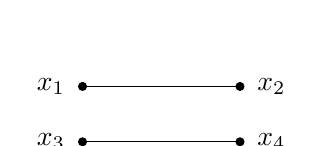
\begin{tikzpicture}[baseline=(r.base)]
      \begin{feynman}[inline=(r.base)]
        \vertex[dot] (a1) {};
        \vertex (l1) at ($(a1)+(-0.4,0)$) {\(x_1\)};
        \vertex[right=2cm of a1, dot] (a2) {};
        \vertex (l2) at ($(a2)+(+0.4,0)$) {\(x_2\)};
        \vertex[below=2em of a1, dot] (b1) {};
        \vertex (l3) at ($(b1)+(-0.4,0)$) {\(x_3\)};
        \vertex[below=2em of a2, dot] (b2) {};
        \vertex (l4) at ($(b2)+(+0.4,0)$) {\(x_4\)};

        \vertex[below=1.2em of a1] (r);

        \diagram* {
          (a1) [dot] -- (a2) [particle = \(x_2\)],
          (b1) [dot] -- (b2) [dot],
        };
      \end{feynman}
    \end{tikzpicture}
   \end{equation*}
   Then, the 4-point Green function can be represented as:
   \begin{equation*}
     \tempord\{\phi(x_1) \phi(x_2) \phi(x_3) \phi(x_4)\}
     =
    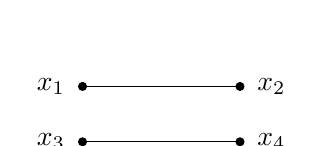
\begin{tikzpicture}[baseline=(r.base)]
      \begin{feynman}[inline=(r.base)]
        \vertex[dot] (a1) {};
        \vertex (l1) at ($(a1)+(-0.4,0)$) {\(x_1\)};
        \vertex[right=2cm of a1, dot] (a2) {};
        \vertex (l2) at ($(a2)+(+0.4,0)$) {\(x_2\)};
        \vertex[below=2em of a1, dot] (b1) {};
        \vertex (l3) at ($(b1)+(-0.4,0)$) {\(x_3\)};
        \vertex[below=2em of a2, dot] (b2) {};
        \vertex (l4) at ($(b2)+(+0.4,0)$) {\(x_4\)};

        \vertex[below=1.1em of a1] (r);

        \diagram* {
          (a1) [dot] -- (a2) [dot],
          (b1) [dot] -- (b2) [dot],
        };
      \end{feynman}
    \end{tikzpicture}
    \ + \
    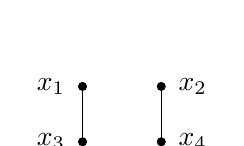
\begin{tikzpicture}[baseline=(r.base)]
      \begin{feynman}[inline=(r.base)]
        \vertex[dot] (a1) {};
        \vertex (l1) at ($(a1)+(-0.4,0)$) {\(x_1\)};
        \vertex[right=1cm of a1, dot] (a2) {};
        \vertex (l2) at ($(a2)+(+0.4,0)$) {\(x_2\)};
        \vertex[below=2em of a1, dot] (b1) {};
        \vertex (l3) at ($(b1)+(-0.4,0)$) {\(x_3\)};
        \vertex[below=2em of a2, dot] (b2) {};
        \vertex (l4) at ($(b2)+(+0.4,0)$) {\(x_4\)};

        \vertex[below=1.1em of a1] (r);

        \diagram* {
          (a1) [dot] -- (b1) [dot],
          (a2) [dot] -- (b2) [dot],
        };
      \end{feynman}
    \end{tikzpicture}
    \ + \
    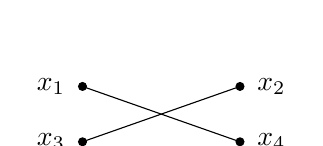
\begin{tikzpicture}[baseline=(r.base)]
      \begin{feynman}[inline=(r.base)]
        \vertex[dot] (a1) {};
        \vertex (l1) at ($(a1)+(-0.4,0)$) {\(x_1\)};
        \vertex[right=2cm of a1, dot] (a2) {};
        \vertex (l2) at ($(a2)+(+0.4,0)$) {\(x_2\)};
        \vertex[below=2em of a1, dot] (b1) {};
        \vertex (l3) at ($(b1)+(-0.4,0)$) {\(x_3\)};
        \vertex[below=2em of a2, dot] (b2) {};
        \vertex (l4) at ($(b2)+(+0.4,0)$) {\(x_4\)};

        \vertex[below=1.1em of a1] (r);

        \diagram* {
          (a1) [dot] -- (b2) [dot],
          (b1) [dot] -- (a2) [dot],
        };
      \end{feynman}
    \end{tikzpicture}
   \end{equation*}
\end{example}

Using this formalism to compute \eref{eq:corr-func-pert}, when expanding the exponential in powers of $ \ham_I $, each term contains fields at the same spacetime point: this gives rise to less trivial Feynman diagrams.

\subsubsection{Fermionic fields}

\begin{definition}{Contraction}{}
  Given a fermionic $ \Psi(x) $, its \bcdef{contraction} is defined as:
  \begin{equation}
    \wick{\c\Psi(x) \c{\bar{\Psi}}(y)} \defeq
    \begin{cases}
      \{\Psi^+(x) , \bar{\Psi}^-(y)\} & x^0 > y^0 \\
      -\{\bar{\Psi}^+(y) , \Psi^-(x)\} & y^0 > x^0
    \end{cases}
  \end{equation}
  and $ \wick{\c\Psi(x) \c\Psi(y)} = \wick{\c{\bar{\Psi}}(x) \c{\bar{\Psi}}(y)} = 0 $.
\end{definition}

By the proof of \tref{th:dirac-prop}, it is clear that:
\begin{equation}
  \tempord\{\Psi(x) \bar{\Psi}(y)\} = \normord\{\Psi(x) \bar{\Psi}(y)\} + \wick{\c\Psi(x) \c{\bar{\Psi}}(y)}
\end{equation}
Wick's theorem remains basically unchanged for fermions.

\begin{theorem}{Wick's theorem}{wick-fermion}
  Given a fermionic field $ \Psi(x) $:
  \begin{equation}
    \tempord\{\Psi(x_1) \bar{\Psi}(x_2) \dots\} = \normord\{\Psi(x_1) \bar{\Psi}(x_2) \dots \,+\, \text{all possible contractions}\}
  \end{equation}
  where both partially-contracted and fully-contracted terms are considered.
\end{theorem}

\begin{proofbox}
  \begin{proof}
    Inserting everything inside $ \normord\{\cdot\} $ ensures that the correct signs are considered due to fermionic anti-commutation, therefore the proof is analogous to that of \tref{th:wick-boson}.
  \end{proof}
\end{proofbox}

As for the bosonic counterparts, only fully-contracted terms contribute to the $ n $-point Green function, as each partially-contracted term will have either an annihilation operator acting on $ \ket{0} $ or a creation operator acting on $ \bra{0} $ (or both).

\subsubsection{Scattering in $ \lambda \phi^4 $-theory}

Consider a real scalar field theory with $ \ham_I = \frac{\lambda}{4!} \phi^4 $ and consider a scattering process with two initial particles with momenta $ \ve{k}_1 , \ve{k}_2 $ and two final particles with momenta $ \ve{p}_1 , \ve{p}_2 $. \eref{eq:lsz-scalar-field} and \eref{eq:corr-func-pert} give the amplitude:
\begin{equation*}
  \begin{split}
    \braket{\ve{p}_1 , \ve{p}_2 | i T | \ve{k}_1 , \ve{k}_2}
    & = \frac{k_1^2 - m^2}{i \sqrt{Z}} \frac{k_2^2 - m^2}{i \sqrt{Z}} \frac{p_1^2 - m^2}{i \sqrt{Z}} \frac{p_2^2 - m^2}{i \sqrt{Z}} \int \prod_{i = 1}^4 \dd^4x_i\, e^{i ({p_1}_\mu {x_1}^\mu + {p_2}_\mu {x_2}^\mu - {p_3}_\mu {x_3}^\mu - {p_4}_\mu {x_4}^\mu)} \times \\
    & \qquad \qquad \times \frac{\braket{0 | \tempord\{ \phi(x_1) \phi(x_2) \phi(x_3) \phi(x_4) \exp \left[ -i \frac{\lambda}{4!} \int \dd^4x\, \phi(x) \right] \} | 0}}{\braket{0 | \tempord\{\exp \left[ - i \frac{\lambda}{4!} \int \dd^4x\, \phi(x) \right]\} | 0}}
  \end{split}
\end{equation*}
To compute this expression up to $ o(\lambda) $, consider that for $ \lambda \phi^4 $-theory $ Z = 1 + o(\lambda^2) $, thus it is safe to set $ Z \equiv 1 $. \\
The $ o(\lambda^0) $ term is obtained setting $ \lambda = 0 $, i.e. no coupling, but in the absence of coupling there is no scattering either and the amplitude must be trivial. Recalling \exref{ex:4-green-func}:
\begin{equation*}
  \begin{split}
    & \int \dd^4x_1 \dd^4x_2 \dd^4x_3 \dd^4x_4\, e^{i ({p_1}_\mu {x_1}^\mu + {p_2}_\mu {x_2}^\mu - {p_3}_\mu {x_3}^\mu - {p_4}_\mu {x_4}^\mu)} \braket{0 | \tempord\{\phi(x_1) \phi(x_2) \phi(x_3) \phi(x_4)\} | 0} \\
    & \qquad = \int \dd^4x_1 \dd^4x_2 \dd^4x_3 \dd^4x_4\, e^{i ({p_1}_\mu {x_1}^\mu + {p_2}_\mu {x_2}^\mu - {p_3}_\mu {x_3}^\mu - {p_4}_\mu {x_4}^\mu)} \left[ D_\text{F}(x_1 - x_2) D_\text{F}(x_3 - x_4) + \dots \right] \\
    & \qquad = \left[ \int \dd^4x \dd^4X\, e^{i (p_1 + p_2)_\mu X^\mu + i (p_1 - p_2)_\mu x^\mu/2} D(x) \right] \left[ \int \dd^4y \dd^4Y\, e^{- i (k_1 + k_2)_\mu Y^\mu - i (k_1 - k_2)_\mu y^\mu/2} D(y) \right] + \dots \\
    & \qquad = (2\pi)^4 \delta^{(4)}(p_1 + p_2) \frac{i}{\left( \frac{p_1 - p_2}{2} \right)^2 - m^2} (2\pi)^4 \delta^{(4)}(k_1 + k_2) \frac{i}{\left( \frac{k_1 - k_2}{2} \right)^2 - m^2} + \dots
  \end{split}
\end{equation*}
with $ x = x_1 - x_2 , 2X = x_1 + x_2 $ and $ y = x_3 - x_4 , 2Y = x_3 + x_4 $. Using $ f(x) \delta(x - x_0) = f(x_0) \delta(x - x_0) $:
\begin{equation*}
  \begin{split}
    & \int \dd^4x_1 \dd^4x_2 \dd^4x_3 \dd^4x_4\, e^{i ({p_1}_\mu {x_1}^\mu + {p_2}_\mu {x_2}^\mu - {p_3}_\mu {x_3}^\mu - {p_4}_\mu {x_4}^\mu)} \braket{0 | \tempord\{\phi(x_1) \phi(x_2) \phi(x_3) \phi(x_4)\} | 0} \\
    & \qquad \qquad \qquad \qquad \qquad \qquad \qquad \qquad = (2\pi)^4 \delta^{(4)}(p_1 + p_2) (2\pi)^4 \delta^{(4)}(k_1 + k_2) \frac{i}{p_1^2 - m^2} \frac{i}{k_1^2 - m^2} + \dots
  \end{split}
\end{equation*}
Note that the $ i\epsilon $ term must be retained while $ p $ is an integration variable, as it gives the prescription of going around the poles, but it can be dropped when $ p $ is the momentum on an external leg, i.e. fixed. This expression only has two poles, therefore:
\begin{equation*}
  \braket{\ve{p}_1 , \ve{p}_2 | i T | \ve{k}_1 , \ve{k}_2} = - (2\pi)^8 \delta^{(4)}(p_1 + p_2) \delta^{(4)}(k_1 + k_2) (p_2^2 - m^2) (k_2^2 - m^2) + \dots + o(\lambda)
\end{equation*}
These terms vanish when going on mass-shell, confirming that at $ o(\lambda^0) $ there is no interaction, i.e. no contribution to the scattering amplitude. This is a general feature of $ n \rightarrow m $ scattering amplitudes: \textit{disconnected graphs do not contribute to the amplitude}, as they do not provide enough pole factors to cancel those in the LSZ formula. \\
The first non-trivial contribution is that at $ o(\lambda) $. The numerator of \eref{eq:corr-func-pert} is:
\begin{equation*}
  \int \prod_{i = 1}^4 \dd^4x_i\, e^{i ({p_1}_\mu {x_1}^\mu + {p_2}_\mu {x_2}^\mu - {p_3}_\mu {x_3}^\mu - {p_4}_\mu {x_4}^\mu)} \left( - i \frac{\lambda}{4!} \right) \int \dd^4x \braket{0 | \tempord\{\phi(x_1) \phi(x_2) \phi(x_3) \phi(x_4) \phi^4(x)\} | 0}
\end{equation*}
The only non-vanishing contribution is the fully-contracted term:
\begin{equation*}
  \braket{0 | \wick{\c1\phi(x_1) \c2\phi(x_2) \c3\phi(x_3) \c4\phi(x_4) \c1\phi(x) \c2\phi(x) \c3\phi(x) \c4\phi(x)} | 0}
  \quad = \quad
  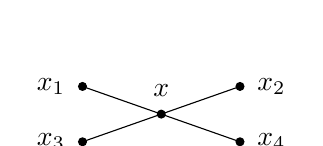
\begin{tikzpicture}[baseline=(r.base)]
    \begin{feynman}[inline=(r.base)]
      \vertex[dot] (a1) {};
      \vertex (l1) at ($(a1)+(-0.4,0)$) {\(x_1\)};
      \vertex[right=2cm of a1, dot] (a2) {};
      \vertex (l2) at ($(a2)+(+0.4,0)$) {\(x_2\)};
      \vertex[below=2em of a1, dot] (b1) {};
      \vertex (l3) at ($(b1)+(-0.4,0)$) {\(x_3\)};
      \vertex[below=2em of a2, dot] (b2) {};
      \vertex (l4) at ($(b2)+(+0.4,0)$) {\(x_4\)};
      \vertex[below=1em of a1] (c1) {};
      \vertex[right=1cm of c1, dot] (c2) {};
      \vertex (l5) at ($(c2)+(0,+0.3)$) {\(x\)};

      \vertex[below=1.1em of a1] (r);

      \diagram* {
        (a1) [dot] -- (b2) [dot],
        (b1) [dot] -- (a2) [dot],
      };
    \end{feynman}
  \end{tikzpicture}
\end{equation*}
as it is the only connected diagram between the possible ones. Note that this diagram corresponds to $ 4! $ equal contractions (only one is shown), therefore the numerator becomes:
\begin{equation*}
  \begin{split}
    & -i \lambda \int \dd^4x \prod_{i = 1}^4 \dd^4x_i\, e^{i ({p_1}_\mu {x_1}^\mu + {p_2}_\mu {x_2}^\mu - {p_3}_\mu {x_3}^\mu - {p_4}_\mu {x_4}^\mu)} D_\text{F}(x_1 - x) D_\text{F}(x_2 - x) D_\text{F}(x_3 - x) D_\text{F}(x_4 - x) \\
    & = -i \lambda \tilde{D}_\text{F}(p_1) \tilde{D}_\text{F}(p_2) \tilde{D}_\text{F}(k_1) \tilde{D}_\text{F}(k_2) \int \dd^4x\, e^{i (p_1 + p_2 - k_1 - k_2)_\mu x^\mu} \\
    & = -i \lambda (2\pi)^4 \delta^{(4)}(p_1 + p_2 - k_1 - k_2) \frac{i}{p_1^2 - m^2} \frac{i}{p_2^2 - m^2} \frac{i}{k_1^2 - m^2} \frac{i}{k_2^2 - m^2}
  \end{split}
\end{equation*}
There remains to evaluate the denominator: this term gives only \bctxt{vacuum-to-vacuum transitions}, i.e. diagrams with no external legs. To account for these, note that each connected diagram which contributes to the numerator can be $ \virgolette{dressed} $ with all possible vacuum-to-vacuum transitions; indeed, to be precise:
\begin{equation*}
  \braket{0 | \wick{\c1\phi(x_1) \c2\phi(x_2) \c3\phi(x_3) \c4\phi(x_4) \c1\phi(x) \c2\phi(x) \c3\phi(x) \c4\phi(x)} | 0} =
\end{equation*}
\begin{equation*}
  = \quad
  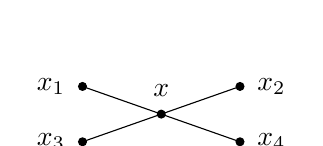
\begin{tikzpicture}[baseline=(r.base)]
    \begin{feynman}[inline=(r.base)]
      \vertex[dot] (a1) {};
      \vertex (l1) at ($(a1)+(-0.4,0)$) {\(x_1\)};
      \vertex[right=2cm of a1, dot] (a2) {};
      \vertex (l2) at ($(a2)+(+0.4,0)$) {\(x_2\)};
      \vertex[below=2em of a1, dot] (b1) {};
      \vertex (l3) at ($(b1)+(-0.4,0)$) {\(x_3\)};
      \vertex[below=2em of a2, dot] (b2) {};
      \vertex (l4) at ($(b2)+(+0.4,0)$) {\(x_4\)};
      \vertex[below=1em of a1] (c1) {};
      \vertex[right=1cm of c1, dot] (c2) {};
      \vertex (l5) at ($(c2)+(0,+0.3)$) {\(x\)};

      \vertex[below=1.1em of a1] (r);

      \diagram* {
        (a1) [dot] -- (b2) [dot],
        (b1) [dot] -- (a2) [dot],
      };
    \end{feynman}
  \end{tikzpicture}
  \quad + \quad
  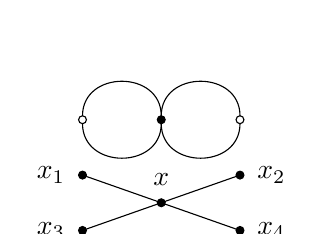
\begin{tikzpicture}[baseline=(r.base)]
    \begin{feynman}[inline=(r.base)]
      \vertex[dot] (a1) {};
      \vertex (l1) at ($(a1)+(-0.4,0)$) {\(x_1\)};
      \vertex[right=2cm of a1, dot] (a2) {};
      \vertex (l2) at ($(a2)+(+0.4,0)$) {\(x_2\)};
      \vertex[below=2em of a1, dot] (b1) {};
      \vertex (l3) at ($(b1)+(-0.4,0)$) {\(x_3\)};
      \vertex[below=2em of a2, dot] (b2) {};
      \vertex (l4) at ($(b2)+(+0.4,0)$) {\(x_4\)};
      \vertex[below=1em of a1] (c1) {};
      \vertex[right=1cm of c1, dot] (c2) {};
      \vertex (l5) at ($(c2)+(0,+0.3)$) {\(x\)};

      \vertex[above=3em of c2, dot] (d1) {};
      \vertex[right=1cm of d1, empty dot] (d2) {};
      \vertex[left=1cm of d1, empty dot] (d3) {};

      \vertex[below=1.1em of a1] (r);

      \diagram* {
        (a1) [dot] -- (b2) [dot],
        (b1) [dot] -- (a2) [dot],

        (d1) -- [half right] (d2) -- [half right] (d1),
        (d1) -- [half left] (d3) -- [half left] (d1),
      };
    \end{feynman}
  \end{tikzpicture}
  \quad + \quad
  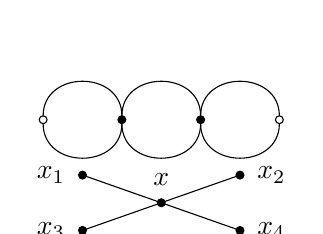
\begin{tikzpicture}[baseline=(r.base)]
    \begin{feynman}[inline=(r.base)]
      \vertex[dot] (a1) {};
      \vertex (l1) at ($(a1)+(-0.4,0)$) {\(x_1\)};
      \vertex[right=2cm of a1, dot] (a2) {};
      \vertex (l2) at ($(a2)+(+0.4,0)$) {\(x_2\)};
      \vertex[below=2em of a1, dot] (b1) {};
      \vertex (l3) at ($(b1)+(-0.4,0)$) {\(x_3\)};
      \vertex[below=2em of a2, dot] (b2) {};
      \vertex (l4) at ($(b2)+(+0.4,0)$) {\(x_4\)};
      \vertex[below=1em of a1] (c1) {};
      \vertex[right=1cm of c1, dot] (c2) {};
      \vertex (l5) at ($(c2)+(0,+0.3)$) {\(x\)};

      \vertex[above=3em of c2] (d0) {};
      \vertex[left=0.5cm of d0, dot] (d1) {};
      \vertex[right=1cm of d1, dot] (d2) {};
      \vertex[left=1cm of d1, empty dot] (d3) {};
      \vertex[right=1cm of d2, empty dot] (d4) {};

      \vertex[below=1.1em of a1] (r);

      \diagram* {
        (a1) [dot] -- (b2) [dot],
        (b1) [dot] -- (a2) [dot],

        (d1) -- [half right] (d2) -- [half right] (d1),
        (d1) -- [half left] (d3) -- [half left] (d1),
        (d2) -- [half right] (d4) -- [half right] (d2),
      };
    \end{feynman}
  \end{tikzpicture}
  \quad + \quad \dots
\end{equation*}
\begin{equation*}
  = \quad
  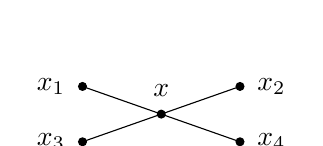
\begin{tikzpicture}[baseline=(r.base)]
    \begin{feynman}[inline=(r.base)]
      \vertex[dot] (a1) {};
      \vertex (l1) at ($(a1)+(-0.4,0)$) {\(x_1\)};
      \vertex[right=2cm of a1, dot] (a2) {};
      \vertex (l2) at ($(a2)+(+0.4,0)$) {\(x_2\)};
      \vertex[below=2em of a1, dot] (b1) {};
      \vertex (l3) at ($(b1)+(-0.4,0)$) {\(x_3\)};
      \vertex[below=2em of a2, dot] (b2) {};
      \vertex (l4) at ($(b2)+(+0.4,0)$) {\(x_4\)};
      \vertex[below=1em of a1] (c1) {};
      \vertex[right=1cm of c1, dot] (c2) {};
      \vertex (l5) at ($(c2)+(0,+0.3)$) {\(x\)};

      \vertex[below=1.1em of a1] (r);

      \diagram* {
        (a1) [dot] -- (b2) [dot],
        (b1) [dot] -- (a2) [dot],
      };
    \end{feynman}
  \end{tikzpicture}
  \quad \times \quad \bigg[ \ 1 \quad + \quad
  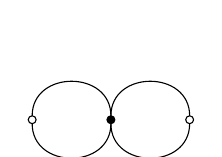
\begin{tikzpicture}[baseline=(r.base)]
    \begin{feynman}[inline=(r.base)]
      \vertex[dot] (d1) {};
      \vertex[right=1cm of d1, empty dot] (d2) {};
      \vertex[left=1cm of d1, empty dot] (d3) {};

      \vertex[below=0.3em of d1] (r);

      \diagram* {
        (d1) -- [half right] (d2) -- [half right] (d1),
        (d1) -- [half left] (d3) -- [half left] (d1),
      };
    \end{feynman}
  \end{tikzpicture}
  \quad + \quad
  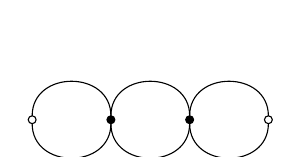
\begin{tikzpicture}[baseline=(r.base)]
    \begin{feynman}[inline=(r.base)]
      \vertex (d0) {};
      \vertex[left=0.5cm of d0, dot] (d1) {};
      \vertex[right=1cm of d1, dot] (d2) {};
      \vertex[left=1cm of d1, empty dot] (d3) {};
      \vertex[right=1cm of d2, empty dot] (d4) {};

      \vertex[below=0.3em of d0] (r);

      \diagram* {
        (d1) -- [half right] (d2) -- [half right] (d1),
        (d1) -- [half left] (d3) -- [half left] (d1),
        (d2) -- [half right] (d4) -- [half right] (d2),
      };
    \end{feynman}
  \end{tikzpicture}
  \quad + \quad \dots \ \bigg]
\end{equation*}
This is nothing but the perturbative expansion of the denominator of \eref{eq:corr-func-pert}, therefore they cancel out leaving only the already computed diagram\footnotemark. Thus, the transition amplitude at $ o(\lambda) $ is:
\begin{equation}
  \braket{\ve{p}_1 , \ve{p}_2 | i T | \ve{k}_1 , \ve{k}_2} = -i \lambda (2\pi)^4 \delta^{(4)}(p_1 + p_2 - k_1 - k_2)
\end{equation}

\footnotetext{This too is a general statement. Consider a generic process with possible connected diagrams $ \{C_i\}_{i \in \mathcal{I}} $ and possible vacuum-to-vacuum diagrams $ \{V_j\}_{j \in \mathcal{J}} $. Then, as shown above, the contribution of a connected diagram $ C_i $ is really:
\begin{equation*}
  C_i \times \sum_{\{n_j\} \subset \N_0} \prod_{j \in \mathcal{J}} \frac{1}{n_j!} V_j^{n_j}
\end{equation*}
with $ \{n_j\}_{j \in \mathcal{J}} \subset \N_0 $ (the symmetry factor is due to the swap of identical diagrams). The sum of all non-vanishing diagrams thus is:
\begin{equation*}
  \begin{split}
    \sum (\text{diagrams})
    & = \sum_{i \in \mathcal{I}} C_i \times \sum_{\{n_j\} \subset \N_0} \prod_{j \in \mathcal{J}} \frac{1}{n_j!} V_j^{n_j} = \sum_{i \in \mathcal{I}} C_i \times \prod_{j \in \mathcal{J}} \sum_{n = 1}^\infty \frac{1}{n!} V_j^n = \sum_{i \in \mathcal{I}} C_i \times \prod_{j \in \mathcal{J}} \exp V_j = \sum_{i \in \mathcal{I}} C_i \times \exp \sum_{j \in \mathcal{J}} V_j
  \end{split}
\end{equation*}
which can be recast in the form:
\begin{equation}
  \sum (\text{diagrams}) = \sum (\text{connected}) \times \exp \sum (\text{vacuum-to-vacuum})
\end{equation}
The exponential exactly cancels $ \braket{0 | \tempord\{\exp \left[ -i \int \dd^4x\, \ham_I \right]\} | 0} $, leaving only connected diagrams in the calculation.}

\subsubsection{Scattering in $ \lambda \phi^3 $-theory}

To illustrate the case of internal lines, it is useful to consider a real scalar field theory with $ \ham_I = \frac{\lambda}{3!} \phi^3 $: in this case, 3 lines meet at each vertex, instead of 4. The $ 2 \rightarrow 2 $ scattering amplitude is:
\begin{equation*}
  \begin{split}
    \braket{\ve{p}_1 , \ve{p}_2 | i T | \ve{k}_1 , \ve{k}_2}
    & = \prod_{i = 1,2} \frac{p_i^2 - m^2}{i \sqrt{Z}} \prod_{j = 1,2} \frac{k_j^2 - m^2}{i \sqrt{Z}} \int \prod_{i = 1}^4 \dd^4x_i\, e^{i ({p_1}_\mu x_1^\mu + {p_2}_\mu x_2^\mu - {k_1}_\mu x_3^\mu - {k_4}_\mu x_4^\mu)} \times \\
    & \qquad \qquad \qquad \qquad \times \braket{0 | \tempord\{\phi(x_1) \phi(x_2) \phi(x_3) \phi(x_4) \exp \left[ -i \frac{\lambda}{3!} \int \dd^4x\, \phi^3(x) \right]\} | 0}
  \end{split}
\end{equation*}
where the denominator was omitted by implicitly considering only connected graphs with 4 external legs. This amplitude does not have a $ o(\lambda^0) $ contribution (as it only has disconnected diagrams) nor an $ o(\lambda) $ contribution (as the product of an odd number of fields cannot be fully contracted). At $ o(\lambda^2) $ the integral becomes:
\begin{equation*}
    \int \prod_{i = 1}^4 \dd^4x_i\, e^{i ({p_1}_\mu x_1^\mu + {p_2}_\mu x_2^\mu - {k_1}_\mu x_3^\mu - {k_4}_\mu x_4^\mu)} \frac{1}{2!} \left( -i \frac{\lambda}{3!} \right)^2 \int \dd^4x \dd^4y \braket{0 | \tempord\{\phi(x_1) \phi(x_2) \phi(x_3) \phi(x_4) \phi^3(x) \phi^3(y)\} | 0}
\end{equation*}
In order to obtain a fully connected diagrams, there needs to be a contraction $ \wick{\c\phi(x) \c\phi(y)} $ between the two vertices, creating an internal line. Note that the $ 1/2! $ factor accounts for the symmetry $ x \leftrightarrow y $, while $ 1/3! $ accounts for sets of equivalent contractions. Examples of possible diagrams are:
\begin{equation*}
  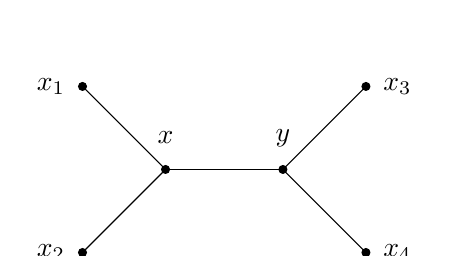
\begin{tikzpicture}[baseline=(r.base)]
    \begin{feynman}[inline=(r.base)]
      \vertex[dot] (x) {};
      \vertex (lx) at ($(x)+(0,0.4)$) {\(x\)};
      \vertex[right=4.242em of x, dot] (y) {};
      \vertex (ly) at ($(y)+(0,0.4)$) {\(y\)};

      \vertex[above=3em of x] (p1) {};
      \vertex[left=3em of p1, dot] (x1) {};
      \vertex (l1) at ($(x1)+(-0.4,0)$) {\(x_1\)};
      \vertex[below=6em of x1, dot] (x2) {};
      \vertex (l2) at ($(x2)+(-0.4,0)$) {\(x_2\)};

      \vertex[above=3em of y] (p2) {};
      \vertex[right=3em of p2, dot] (x3) {};
      \vertex (l3) at ($(x3)+(0.4,0)$) {\(x_3\)};
      \vertex[below=6em of x3, dot] (x4) {};
      \vertex (l4) at ($(x4)+(0.4,0)$) {\(x_4\)};

      \vertex[below=0.3em of x] (r) {};

      \diagram* {
        (x1) -- (x) -- (y) -- (x3),
        (x2) -- (x),
        (y) -- (x4),
      };
    \end{feynman}
  \end{tikzpicture}
  \quad = \quad
  D_\text{F}(x_1 - x) D_\text{F}(x_2 - x) D_\text{F}(x - y) D_\text{F}(y - x_3) D_\text{F}(y - x_4)
\end{equation*}
\begin{equation*}
  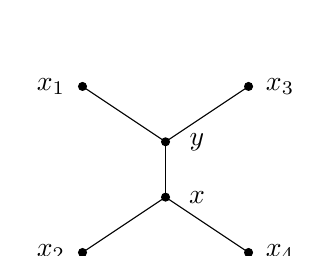
\begin{tikzpicture}[baseline=(r.base)]
    \begin{feynman}[inline=(r.base)]
      \vertex[dot] (x) {};
      \vertex (lx) at ($(x)+(0.4,0)$) {\(x\)};
      \vertex[above=2em of x, dot] (y) {};
      \vertex (ly) at ($(y)+(0.4,0)$) {\(y\)};

      \vertex[above=2em of y] (p1) {};
      \vertex[left=3em of p1, dot] (x1) {};
      \vertex (l1) at ($(x1)+(-0.4,0)$) {\(x_1\)};
      \vertex[below=6em of x1, dot] (x2) {};
      \vertex (l2) at ($(x2)+(-0.4,0)$) {\(x_2\)};

      \vertex[right=3em of p1, dot] (x3) {};
      \vertex (l3) at ($(x3)+(0.4,0)$) {\(x_3\)};
      \vertex[below=6em of x3, dot] (x4) {};
      \vertex (l4) at ($(x4)+(0.4,0)$) {\(x_4\)};

      \vertex[above=0.7em of x] (r) {};

      \diagram* {
        (x1) -- (y) -- (x3),
        (x) -- (y),
        (x2) -- (x) -- (x4),
      };
    \end{feynman}
  \end{tikzpicture}
  \quad = \quad
  D_\text{F}(x_1 - y) D_\text{F}(x_2 - x) D_\text{F}(x - y) D_\text{F}(y - x_3) D_\text{F}(x - x_4)
\end{equation*}
These diagrams are inequivalent, as they correspond to different sets of contractions. Computing for example the first one:
\begin{equation*}
  \begin{split}
    & (-i \lambda)^2 \int \prod_{i = 1}^4 \dd^4x_i\, e^{i ({p_1}_\mu x_1^\mu + {p_2}_\mu x_2^\mu - {k_1}_\mu x_3^\mu - {k_4}_\mu x_4^\mu)} \times \\
    & \qquad \qquad \qquad \qquad \qquad \qquad \times \int \dd^4x \dd^4y\, D_\text{F}(x_1 - x) D_\text{F}(x_2 - x) D_\text{F}(x - y) D_\text{F}(y - x_3) D_\text{F}(y - x_4) \\
    & = (-i \lambda)^2 \tilde{D}_\text{F}(p_1) \tilde{D}_\text{F}(p_2) \tilde{D}_\text{F}(k_1) \tilde{D}_\text{F}(k_2) \int \dd^4x \dd^4y\, e^{i (p_1 + p_2)_\mu x^\mu - i (k_1 + k_2)_\mu y^\mu} D_\text{F}(x - y) \\
    & = (-i \lambda)^2 \tilde{D}_\text{F}(p_1) \tilde{D}_\text{F}(p_2) \tilde{D}_\text{F}(k_1) \tilde{D}_\text{F}(k_2) \int \dd^4X \dd^4Y\, e^{i (p_1 + p_2 - k_1 - k_2)_\mu Y^\mu + i (p_1 + p_2 + k_1 + k_2)_\mu X^\mu / 2} D_\text{F}(X) \\
    & = (-i \lambda)^2 (2\pi)^4 \delta^{(4)}(p_1 + p_2 - k_1 - k_2) \tilde{D}_\text{F}(p_1) \tilde{D}_\text{F}(p_2) \tilde{D}(p_1 + p_2) \tilde{D}_\text{F}(k_1) \tilde{D}_\text{F}(k_2)
  \end{split}
\end{equation*}
with $ X = x - y , 2Y = x + y $. As expected, momentum-space propagators associated to external legs are canceled by pole terms in the LSZ formula: now there remains only the $ \tilde{D}_\text{F}(p_1 + p_2) $ factor associated to the internal line. \\
It is useful to work in momentum space, rather than coordinate space. For example, in momentum space the above diagrams become:
\begin{equation*}
  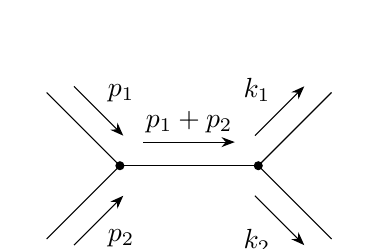
\begin{tikzpicture}[baseline=(r.base)]
    \begin{feynman}[inline=(r.base)]
      \vertex[dot] (x) {};
      \vertex[right=5em of x, dot] (y) {};

      \vertex[above=3em of x] (p1) {};
      \vertex[left=3em of p1] (x1) {};
      \vertex[below=6em of x1] (x2) {};

      \vertex[above=3em of y] (p2) {};
      \vertex[right=3em of p2] (x3) {};
      \vertex[below=6em of x3] (x4) {};

      \vertex[below=0.3em of x] (r) {};

      \diagram* {
        (x1) -- [momentum = \(p_1\)] (x) -- [momentum = \(p_1 + p_2\)] (y) -- [momentum = \(k_1\)] (x3),
        (x2) -- [momentum' = \(p_2\)] (x),
        (y) -- [momentum' = \(k_2\)] (x4),
      };
    \end{feynman}
  \end{tikzpicture}
  \qquad \qquad \qquad \qquad
  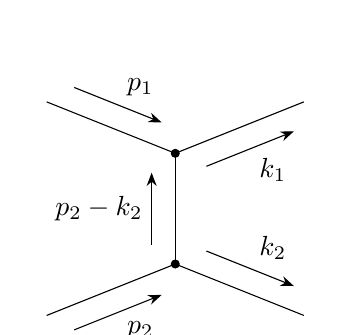
\begin{tikzpicture}[baseline=(r.base)]
    \begin{feynman}[inline=(r.base)]
      \vertex[dot] (x) {};
      \vertex[above=4em of x, dot] (y) {};

      \vertex[above=2em of y] (p1) {};
      \vertex[left=5em of p1] (x1) {};
      \vertex[below=8em of x1] (x2) {};

      \vertex[right=5em of p1] (x3) {};
      \vertex[below=8em of x3] (x4) {};

      \vertex[above=1.7em of x] (r) {};

      \diagram* {
        (x1) -- [momentum = \(p_1\)] (y) -- [momentum' = \(k_1\)] (x3),
        (x) -- [momentum = \(p_2 - k_2\)] (y),
        (x2) -- [momentum' = \(p_2\)] (x) -- [momentum = \(k_2\)] (x4),
      };
    \end{feynman}
  \end{tikzpicture}
\end{equation*}

\subsubsection{General considerations}

The example calculations carried for $ \lambda \phi^3 $- and $ \lambda \phi^4 $-theory hint to the general technique to compute general \bctxt{tree diagrams}, i.e. connected diagrams without internal loops. For a scalar field theory, in momentum space:
\begin{enumerate}
  \item draw all possible connected graphs corresponding to the given initial and final states;
  \item each external leg is associated to a pole factor in the LSZ reduction formula, hence they can be omitted directly ($ \virgolette{leg amputation} $);
  \item as there is always a momentum-conserving $ \delta $-function, it is convenient to define the matrix element $ \mat_\text{if} $ for the process $ \ket{\text{i}} \rightarrow \ket{\text{f}} $ as:
    \begin{equation}
      \braket{\ve{p}_1 , \dots , \ve{p}_m | i T | \ve{k}_1 , \dots , \ve{k}_n} \equiv (2\pi)^4 \delta^{(4)}\left( \sum_{i = 1}^{m} p_i - \sum_{j = 1}^{n} k_j \right) i \mat_\text{if}
      \label{eq:mat-el}
    \end{equation}
  \item energy-momentum conservation must be imposed separately at each vertex;
  \item each vertex is associated to a $ -i \lambda $ factor, where $ \lambda $ is the coupling constant of the interaction;
  \item check if that symmetry factors cancel fully or partially with the $ 1/n! $ factor at $ o(\lambda^n) $ and possible numerical factors in the definition of $ \ham_I $.
\end{enumerate}

\subsection{Loop diagrams}

To illustrate how loop diagrams are treated, consider the $ o(\lambda^2) $ corrections to the $ 2 \rightarrow 2 $ scattering in $ \lambda \phi^4 $-theory:
\begin{multline*}
  \frac{1}{2!} \left( -i \frac{\lambda}{4!} \right)^2 \int \prod_{i = 1}^4 \dd^4x_i\, e^{i ({p_1}_\mu x_1^\mu + {p_2}_\mu x_2^\mu - {k_1}_\mu x_3^\mu - {k_4}_\mu x_4^\mu)} \times \\
  \times \int \dd^4x \dd^4y \braket{0 | \tempord\{\phi(x_1) \phi(x_2) \phi(x_3) \phi(x_4) \phi^4(x) \phi^4(y)\} | 0}
\end{multline*}
There are three possible inequivalent full contractions, associated to the connected diagrams:
\begin{equation*}
  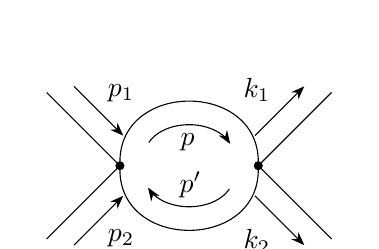
\begin{tikzpicture}[baseline = (r.base)]
    \begin{feynman}[inline = (r.base)]
      \vertex (x1) {};
      \vertex[below=3em of x1] (p1) {};
      \vertex[below=3em of p1] (x2) {};

      \vertex[right=3em of p1, dot] (v1) {};
      \vertex[right=5em of v1, dot] (v2) {};

      \vertex[right=3em of v2] (p2) {};
      \vertex[above=3em of p2] (x3) {};
      \vertex[below=3em of p2] (x4) {};

      \vertex[above=0.5em of v1] (r) {};

      \diagram* {
        (x1) -- [momentum = \(p_1\)] (v1),
        (x2) -- [momentum' = \(p_2\)] (v1),
        (v2) -- [momentum = \(k_1\)] (x3),
        (v2) -- [momentum' = \(k_2\)] (x4),

        (v1) -- [half left, momentum' = \(p\)] (v2),
        (v2) -- [half left, momentum' = \(p'\)] (v1),
      };
    \end{feynman}
  \end{tikzpicture}
  \qquad
  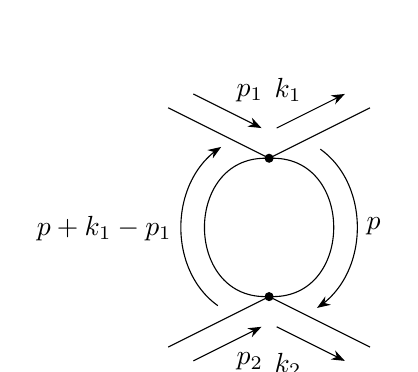
\begin{tikzpicture}[baseline = (r.base)]
    \begin{feynman}[inline = (r.base)]
      \vertex (x1) {};
      \vertex[right=4em of x1] (p1) {};
      \vertex[right=4em of p1] (x3) {};

      \vertex[below=2em of p1, dot] (v1) {};
      \vertex[below=5em of v1, dot] (v2) {};

      \vertex[below=9em of x1] (x2) {};
      \vertex[below=9em of x3] (x4) {};

      \vertex[below=2em of v1] (r) {};

      \diagram* {
        (x1) -- [momentum = \(p_1\)] (v1) -- [momentum = \(k_1\)] (x3),
        (x2) -- [momentum' = \(p_2\)] (v2) -- [momentum' = \(k_2\)] (x4),

        (v1) -- [half left, momentum = \(p\)] (v2),
        (v2) -- [half left, momentum = \(p + k_1 - p_1\)] (v1),
      };
    \end{feynman}
  \end{tikzpicture}
  \qquad
  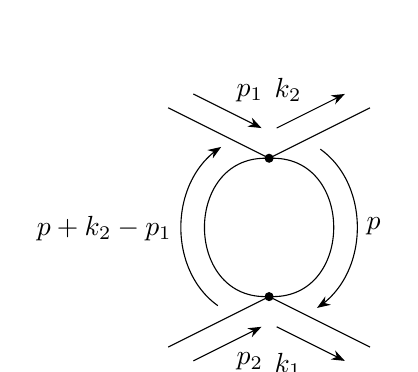
\begin{tikzpicture}[baseline = (r.base)]
    \begin{feynman}[inline = (r.base)]
      \vertex (x1) {};
      \vertex[right=4em of x1] (p1) {};
      \vertex[right=4em of p1] (x3) {};

      \vertex[below=2em of p1, dot] (v1) {};
      \vertex[below=5em of v1, dot] (v2) {};

      \vertex[below=9em of x1] (x2) {};
      \vertex[below=9em of x3] (x4) {};

      \vertex[below=2em of v1] (r) {};

      \diagram* {
        (x1) -- [momentum = \(p_1\)] (v1) -- [momentum = \(k_2\)] (x3),
        (x2) -- [momentum' = \(p_2\)] (v2) -- [momentum' = \(k_1\)] (x4),

        (v1) -- [half left, momentum = \(p\)] (v2),
        (v2) -- [half left, momentum = \(p + k_2 - p_1\)] (v1),
      };
    \end{feynman}
  \end{tikzpicture}
\end{equation*}
with $ p' = p_1 + p_2 - p $. It is clear that energy conservation does not completely fix momenta of internal lines, and in particular of loops.
Consider for example the first diagram: it is obtained contracting $ \phi(x_1) $ and $ \phi(x_2) $ with two $ \phi(x) $ ($ 4 \cdot 3 $ ways), $ \phi(x_3) $ and $ \phi(x_4) $ with two $ \phi(y) $ ($ 4 \cdot 3 $ ways) and two $ \phi(x) $ with two $ \phi(y) $ ($ 2 $ ways), so, considering another $ 2 $ factor for $ x \leftrightarrow y $ symmetry, this diagram has symmetry number $ S = (4!)^2 $. The resulting contribution is:
\begin{equation*}
  \begin{split}
    & \frac{(-i \lambda)^2}{2} \int \prod_{i = 1}^4 \dd^4x_i\, e^{i ({p_1}_\mu x_1^\mu + {p_2}_\mu x_2^\mu - {k_1}_\mu x_3^\mu - {k_4}_\mu x_4^\mu)} \int \dd^4x \dd^4y D_\text{F}(x_1 - x) D_\text{F}(x_2 - x) D_\text{F}(x - y) D_\text{F}(y - x) \\
    & = \frac{(-i \lambda)^2}{2} \tilde{D}_\text{F}(p_1) \tilde{D}_\text{F}(p_2) \tilde{D}_\text{F}(k_1) \tilde{D}_\text{F}(k_2) \int \dd^4x \dd^4y\, e^{i (p_1 + p_2)_\mu x^\mu - i (k_1 + k_2)_\mu y^\mu} D^2(x - y) \\
    & = \frac{(-i \lambda)^2}{2} \tilde{D}_\text{F}(p_1) \tilde{D}_\text{F}(p_2) \tilde{D}_\text{F}(k_1) \tilde{D}_\text{F}(k_2) (2\pi)^4 \delta^{(4)}(p_1 + p_2 - k_1 - k_2) \int \frac{\dd^4k}{(2\pi)^4} \tilde{D}_\text{F}(k) \tilde{D}_\text{F}(p_1 + p_2 - k)
  \end{split}
\end{equation*}
Therefore, the additional feature of loop integrals is the integration over unfixed momenta, assigning the right propagators to each internal line. It is possible to define the \bctxt{loop-amplitude} for $ \lambda \phi^4 $-theory:
\begin{equation}
  \mathcal{A}(p) \defeq \frac{(-i \lambda)^2}{2} \int \frac{\dd^4k}{(2\pi)^4} \frac{i}{k^2 - m^2 + i \epsilon} \frac{i}{(p - k)^2 - m^2 + i \epsilon}
  \label{eq:f4-loop-ampl}
\end{equation}
so that the $ 2 \rightarrow 2 $ scattering amplitude at one-loop level (i.e. $ o(\lambda^2) $) is:
\begin{equation}
  i \mat_{2 \rightarrow 2} = -i \lambda + \mathcal{A}(p_1 + p_2) + \mathcal{A}(p_1 - k_1) + \mathcal{A}(p_1 - k_2)
\end{equation}

\subsubsection{Divergences}

The integral in \eref{eq:f4-loop-ampl} diverges at large $ k $, which is an example of \bctxt{UV divergence}. To study this divergence, first of all note that $ (p - k)^2 \rightarrow k^2 $ as $ k \rightarrow \infty $, so that it is safe to set $ p = 0 $. Due to the $ i\epsilon $-presciption, in the complex $ k^0 $-plane the pole in $ k^0 > 0 $ is below the real axis, while that in $ k^0 < 0 $ is above it: the integration path can then be rotated counterclockwise from the real axis to the imaginary axis by $ k^0 \mapsto i k^0 $, which is called a \bctxt{Wick rotation}. The amplitude then becomes:
\begin{equation*}
    \mathcal{A}(0) = \frac{(-i \lambda)^2}{2} \int \frac{\dd^4k}{(2\pi)^4} \left( \frac{i}{k^2 - m^2 + i\epsilon} \right)^2 \mapsto i \frac{\lambda^2}{2} \int \frac{\dd^4k}{(2\pi)^4} \frac{1}{(k^2 + m^2)^2}
\end{equation*}
where $ k^2 = k_0^2 + \ve{k}^2 $ is now a Euclidean momentum. To regulate the UV divergence, a cutoff $ \Lambda : k^2 < \Lambda^2 $ is introduced, so that:
\begin{equation*}
  \begin{split}
    \mathcal{A}(0)
    & = i \frac{\lambda^2}{2} \int \frac{\dd^4k}{(2\pi)^4} \frac{1}{k^4} + \text{finite terms} = i \frac{\lambda^2}{2} \frac{1}{(2\pi)^4} 2\pi^2 \int^\Lambda \frac{\dd k}{k} + \text{finite terms}\\
    & = \frac{i \lambda^2}{16 \pi^2} \log \Lambda + \text{finite terms}
  \end{split}
\end{equation*}
where $ 2\pi^2 $ is the solid angle in $ \R^4 $. It can be shown that, for general $ p $, the singular part of $ \mathcal{A}(p) $ does not depend on $ p $; hence, it can be written:
\begin{equation*}
  i \mat_{2 \rightarrow 2} = -i \lambda + i \lambda^2 \left( \beta_0 \log \Lambda + \text{finite terms} \right)
\end{equation*}
where:
\begin{equation}
  \beta_0 \equiv \frac{3}{16 \pi^2}
\end{equation}
Another example of loop divergence in $ \lambda \phi^4 $-theory is that associated to the 2-point Green function at $ o(\lambda^1) $:
\begin{equation*}
  \braket{0 | \tempord\{\phi(x_1) \phi(x_2) \phi^4(x)\} | 0} = 4\cdot3 \cdot \wick{\c1\phi(x_1) \c2\phi(x_2) \c1\phi(x) \c2\phi(x) \c1\phi(x) \c1\phi(x)} = \ 4\cdot3 \ \times \
  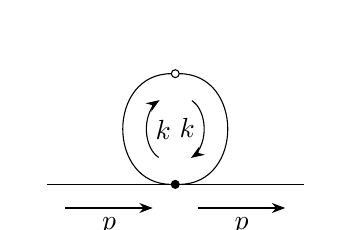
\begin{tikzpicture}[baseline = (r.base)]
    \begin{feynman}[inline = (r.base)]
      \vertex (x1) {};
      \vertex[right=5em of x1, dot] (v1) {};
      \vertex[above=4em of v1, empty dot] (v2) {};
      \vertex[right=5em of v1] (x2) {};

      \vertex[below=0.2em of v1] (r) {};

      \diagram* {
        (x1) -- [momentum' = \(p\)] (v1) -- [momentum' = \(p\)] (x2),
        (v1) -- [half left, momentum' = \(k\)] (v2),
        (v2) -- [half left, momentum' = \(k\)] (v1),
      };
    \end{feynman}
  \end{tikzpicture}
\end{equation*}
This diagram is typically called a \bctxt{tadpole}. Its contribution can be computed in momentum performing a Wick rotation:
\begin{equation}
  -i B \equiv \frac{-i \lambda}{2} \int \frac{\dd^4k}{(2\pi)^4} \frac{1}{k^2 + m^2} = - i \frac{\lambda}{32\pi^2} \left( \Lambda^2 - m^2 \log \frac{\Lambda^2 + m^2}{m^2} \right)
\end{equation}
Note that the tadpole is independent of $ p $, and it has both a quadratic and logarithmic UV divergence.

\begin{lemma}{Tadpole resummation}{}
  In $ \lambda \phi^4 $-theory, for a $ \ket{\ve{p}} \rightarrow \ket{\ve{p}} $ scattering, tadpole diagrams collectively contribute as:
  \begin{equation*}
    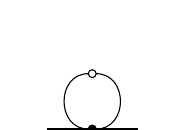
\begin{tikzpicture}[baseline = (r.base)]
      \begin{feynman}[inline = (r.base)]
        \vertex (x1) {};
        \vertex[right=2em of x1, dot] (v1) {};
        \vertex[above=2em of v1, empty dot] (v2) {};
        \vertex[right=2em of v1] (x2) {};

        \vertex[below=0.2em of v1] (r) {};

        \diagram* {
          (x1) -- (v1) -- (x2),

          (v1) -- [half left] (v2),
          (v2) -- [half left] (v1),
        };
      \end{feynman}
    \end{tikzpicture}
    \quad + \quad
    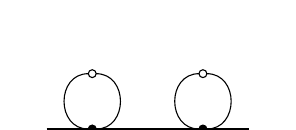
\begin{tikzpicture}[baseline = (r.base)]
      \begin{feynman}[inline = (r.base)]
        \vertex (x1) {};
        \vertex[right=2em of x1, dot] (v1) {};
        \vertex[above=2em of v1, empty dot] (v2) {};
        \vertex[right=4em of v1, dot] (v3) {};
        \vertex[above=2em of v3, empty dot] (v4) {};
        \vertex[right=2em of v3] (x2) {};

        \vertex[below=0.2em of v1] (r) {};

        \diagram* {
          (x1) -- (v1) -- (v3) -- (x2),

          (v1) -- [half left] (v2),
          (v2) -- [half left] (v1),

          (v3) -- [half left] (v4),
          (v4) -- [half left] (v3),
        };
      \end{feynman}
    \end{tikzpicture}
    \quad + \quad
    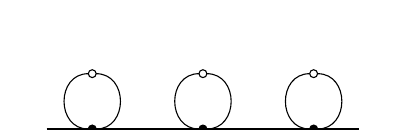
\begin{tikzpicture}[baseline = (r.base)]
      \begin{feynman}[inline = (r.base)]
        \vertex (x1) {};
        \vertex[right=2em of x1, dot] (v1) {};
        \vertex[above=2em of v1, empty dot] (v2) {};
        \vertex[right=4em of v1, dot] (v3) {};
        \vertex[above=2em of v3, empty dot] (v4) {};
        \vertex[right=4em of v3, dot] (v5) {};
        \vertex[above=2em of v5, empty dot] (v6) {};
        \vertex[right=2em of v5] (x2) {};

        \vertex[below=0.2em of v1] (r) {};

        \diagram* {
          (x1) -- (v1) -- (v3) -- (v5) -- (x2),

          (v1) -- [half left] (v2),
          (v2) -- [half left] (v1),

          (v3) -- [half left] (v4),
          (v4) -- [half left] (v3),

          (v5) -- [half left] (v6),
          (v6) -- [half left] (v5),
        };
      \end{feynman}
    \end{tikzpicture}
    \quad + \quad \dots
  \end{equation*}
  \begin{equation*}
    = \frac{i}{p^2 - m^2 - B}
  \end{equation*}
\end{lemma}

\begin{proofbox}
  \begin{proof}
    The represented diagram series reduces to a geometric series in momentum space:
    \begin{equation*}
      \begin{split}
        & \tilde{D}_\text{F}(p) + \tilde{D}_\text{F}(p) (-iB) \tilde{D}_\text{F}(p) + \tilde{D}_\text{F}(p) (-iB) \tilde{D}_\text{F}(p) (-iB) \tilde{D}_\text{F}(p) + \dots \\
        & = \tilde{D}_\text{F}(p) \sum_{n = 0}^{\infty} \left[ -i B \tilde{D}_\text{F}(p) \right]^n = \tilde{D}_\text{F} \frac{1}{1 + i B \tilde{D}_\text{F}(p)} = \frac{i}{p^2 - m^2} \left[ 1 - \frac{B}{p^2 - m^2} \right]^{-1} = \frac{i}{p^2 - m^2 - B}
      \end{split}
    \end{equation*}
    which is the thesis.
  \end{proof}
\end{proofbox}

This shows that accounting for tadpole diagrams is equivalent to shifting the mass $ m^2 \mapsto m^2 + B $.

\subsection{Feynman rules}

To compute amplitudes up to a desired order, it is not necessary to explicitly expanding the exponential each time and then performing Wick contractions, as these steps are summarized by a simple set of rules.

\subsubsection{$ \lambda \phi^n $-theory}

Consider a scalar field theory with Hamiltonian:
\begin{equation}
  \ham = \ham_\text{KG} + \frac{\lambda}{n!} \phi^n
\end{equation}
The Feynman rules in momentum space for this theory are:
\begin{enumerate}
  \item for each internal line:
    $
    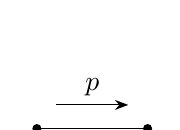
\begin{tikzpicture}[baseline = (r.base)]
      \begin{feynman}[inline = (r.base)]
        \vertex[dot] (x) {};
        \vertex[right=4em of x, dot] (y) {};

        \vertex[below=0.2em of x] (r) {};

        \diagram* {
          (x) -- [momentum = \(p\)] (y),
        };
      \end{feynman}
    \end{tikzpicture}
    = \tilde{D}_\text{F}(p)
    $;
  \item for each external leg:
    $
    \begin{tikzpicture}[baseline = (r.base)]
      \begin{feynman}[inline = (r.base)]
        \vertex[dot] (x) {};
        \vertex[right=4em of x] (y) {};

        \vertex[below=0.2em of x] (r) {};

        \diagram* {
          (x) -- (y),
        };
      \end{feynman}
    \end{tikzpicture}
    = 1
    $;
  \item for each vertex:
    $
    \begin{tikzpicture}[baseline = (r.base)]
      \begin{feynman}[inline = (r.base)]
        \vertex[dot] (x) {};
      \end{feynman}
    \end{tikzpicture}
    = -i \lambda
    $;
  \item impose momentum conservation at each vertex;
  \item integrate over each undetermined loop momentum $ p $ with measure $ \frac{\dd^4p}{(2\pi)^4} $;
  \item divide by the symmetry factor of the diagram.
\end{enumerate}

The problem of computing scattering amplitude is thus reduced to that of drawing every inequivalent fully-connected Feynman diagram (modulo void-to-void diagrams). These rules allow to compute the matrix element $ \mat_\text{if} $, which is related to the $ T $-matrix element by \eref{eq:mat-el} and to the $ S $-matrix element by $ S = 1 + i T $.

\subsubsection{Yukawa theory}

Consider a field theory with a real scalar field $ \phi(x) $ and a Dirac field $ \Psi(x) $. The \bctxt{Yukawa Hamiltonian} is:
\begin{equation}
  \ham = \ham_\text{KG} + \ham_\text{D} + g \bar{\Psi} \Psi \phi
\end{equation}
where $ g $ is a dimensionless coupling constant. This is a simplified model of QED. Note that the form of $ \ham_\text{int} $ allows interaction vertices with two fermion lines and one scalar line. The Feynman rules in momentum space for this theory are:
\begin{enumerate}
  \item propagators:
    \begin{enumerate}
      \item scalar:
      $
      \begin{tikzpicture}[baseline = (r.base)]
        \begin{feynman}[inline = (r.base)]
          \vertex[dot] (x) {};
          \vertex[right=4em of x, dot] (y) {};

          \vertex[below=0.2em of x] (r) {};

          \diagram* {
            (x) -- [scalar, momentum = \(q\)] (y),
          };
        \end{feynman}
      \end{tikzpicture}
      \,=\, \displaystyle\frac{i}{q^2 - m_\phi^2 + i\epsilon} = \tilde{D}_\text{F}(q)
      $;
      \item fermion:
      $
      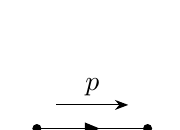
\begin{tikzpicture}[baseline = (r.base)]
        \begin{feynman}[inline = (r.base)]
          \vertex[dot] (x) {};
          \vertex[right=4em of x, dot] (y) {};

          \vertex[below=0.2em of x] (r) {};

          \diagram* {
            (x) -- [fermion, momentum = \(p\)] (y),
          };
        \end{feynman}
      \end{tikzpicture}
      \,=\, \displaystyle\frac{i(\slashed{p} + m)}{p^2 - m^2 + i\epsilon} = \tilde{S}_\text{D}(p)
      $;
    \end{enumerate}
  \item vertex:
    $
    \begin{tikzpicture}[baseline = (r.base)]
      \begin{feynman}[inline = (r.base)]
        \vertex[dot] (x) {};
        \vertex[right=4em of x] (y) {};

        \vertex[above=2em of x] (p) {};
        \vertex[left=2em of p] (p1) {};
        \vertex[below=4em of p1] (p2) {};

        \vertex[below=0.2em of x] (r) {};

        \diagram* {
          (x) -- [scalar] (y),
          (p2) -- [fermion] (x) -- [fermion] (p1),
        };
      \end{feynman}
    \end{tikzpicture}
    \,=\, -i g
    $;
  \item external legs:
    \begin{enumerate}
      \item initial state:
        \begin{enumerate}
          \item scalar:
            $
            \begin{tikzpicture}[baseline = (r.base)]
              \begin{feynman}[inline = (r.base)]
                \vertex[dot] (x) {};
                \vertex[right=4em of x] (y) {};

                \vertex[above=1em of x] (p) {};
                \vertex[left=1em of p] (p1) {};
                \vertex[below=2em of p1] (p2) {};

                \vertex[below=0.2em of x] (r) {};

                \diagram* {
                  (y) -- [scalar, momentum = \(q\)] (x),
                  (p2) -- (x) -- (p1),
                };
              \end{feynman}
            \end{tikzpicture}
            \,=\, 1
            $;
          \item fermion:
            $
            \begin{tikzpicture}[baseline = (r.base)]
              \begin{feynman}[inline = (r.base)]
                \vertex[dot] (x) {};
                \vertex[right=4em of x] (y) {};

                \vertex[above=1em of x] (p) {};
                \vertex[left=1em of p] (p1) {};
                \vertex[below=2em of p1] (p2) {};

                \vertex[below=0.2em of x] (r) {};

                \diagram* {
                  (y) -- [fermion, momentum = \(p\)] (x),
                  (p2) -- (x) -- (p1),
                };
              \end{feynman}
            \end{tikzpicture}
            \,=\, u^s(p)
            $;
          \item anti-fermion:
            $
            \begin{tikzpicture}[baseline = (r.base)]
              \begin{feynman}[inline = (r.base)]
                \vertex[dot] (x) {};
                \vertex[right=4em of x] (y) {};

                \vertex[above=1em of x] (p) {};
                \vertex[left=1em of p] (p1) {};
                \vertex[below=2em of p1] (p2) {};

                \vertex[below=0.2em of x] (r) {};

                \diagram* {
                  (y) -- [anti fermion, momentum = \(k\)] (x),
                  (p2) -- (x) -- (p1),
                };
              \end{feynman}
            \end{tikzpicture}
            \,=\, \bar{v}^s(k)
            $;
        \end{enumerate}
      \item final state:
        \begin{enumerate}
          \item scalar:
            $
            \begin{tikzpicture}[baseline = (r.base)]
              \begin{feynman}[inline = (r.base)]
                \vertex[dot] (x) {};
                \vertex[right=4em of x] (y) {};

                \vertex[above=1em of x] (p) {};
                \vertex[left=1em of p] (p1) {};
                \vertex[below=2em of p1] (p2) {};

                \vertex[below=0.2em of x] (r) {};

                \diagram* {
                  (x) -- [scalar, momentum' = \(q\)] (y),
                  (p2) -- (x) -- (p1),
                };
              \end{feynman}
            \end{tikzpicture}
            \,=\, 1
            $;
          \item fermion:
            $
            \begin{tikzpicture}[baseline = (r.base)]
              \begin{feynman}[inline = (r.base)]
                \vertex[dot] (x) {};
                \vertex[right=4em of x] (y) {};

                \vertex[above=1em of x] (p) {};
                \vertex[left=1em of p] (p1) {};
                \vertex[below=2em of p1] (p2) {};

                \vertex[below=0.2em of x] (r) {};

                \diagram* {
                  (x) -- [fermion, momentum' = \(p\)] (y),
                  (p2) -- (x) -- (p1),
                };
              \end{feynman}
            \end{tikzpicture}
            \,=\, \bar{u}^s(p)
            $;
          \item anti-fermion:
            $
            \begin{tikzpicture}[baseline = (r.base)]
              \begin{feynman}[inline = (r.base)]
                \vertex[dot] (x) {};
                \vertex[right=4em of x] (y) {};

                \vertex[above=1em of x] (p) {};
                \vertex[left=1em of p] (p1) {};
                \vertex[below=2em of p1] (p2) {};

                \vertex[below=0.2em of x] (r) {};

                \diagram* {
                  (x) -- [anti fermion, momentum' = \(k\)] (y),
                  (p2) -- (x) -- (p1),
                };
              \end{feynman}
            \end{tikzpicture}
            \,=\, v^s(k)
            $;
        \end{enumerate}
    \end{enumerate}
  \item impose momentum conservation at each vertex;
  \item integrate over each undetermined loop momentum $ p $ with measure $ \frac{\dd^4p}{(2\pi)^4} $ (each closed fermionic loop determines an additional $ (-1) $ factor due to anti-commutation);
  \item divide by the symmetry factor of the diagram.
\end{enumerate}
Note that for the Yukawa interaction $ g \bar{\Psi} \Psi \phi $ the symmetry factor of each diagram is $ S = 1 $, as the three field in $ \ham_\text{int} $ cannot substitute for one another in contractions. Moreover, Dirac indices are always contracted together along fermionic lines. \\
It can be shown that an interaction mediated by a scalar field is always attractive, both for $ ff $, $ f\bar{f} $ and $ \bar{f}\bar{f} $ scattering.

\subsubsection{Quantum Electrodynamics}

Consider a field theory with a Dirac field $ \Psi(x) $ and a vector (gauge) field $ A_\mu(x) $. The \bctxt{QED interaction Hamiltonian} is:
\begin{equation}
  \ham_\text{int} = e \bar{\Psi} \gamma^\mu \Psi A_\mu
\end{equation}
This interaction term determines interaction vertices with two fermionic lines and one vector line.
The photon propagator is introduced:
\begin{equation}
  D_{\mu \nu}(x-y) \defeq \braket{0 | \tempord\{A_\mu(x) A_\nu(y)\} | 0}
  \qquad \Rightarrow \qquad
  \tilde{D}_{\mu \nu}(k) = \frac{-i}{k^2 + i\epsilon} \eta_{\mu \nu}
\end{equation}
Note that the spatial components $ A_i(x) $ have the same propagator as a massless real scalar field, while $ A_0(x) $ has an additional negative sign.
The Feynman rules in momentum space for QED are:
\begin{enumerate}
  \item propagators:
    \begin{enumerate}
      \item vector:
      $
      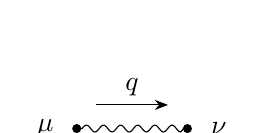
\begin{tikzpicture}[baseline = (r.base)]
        \begin{feynman}[inline = (r.base)]
          \vertex[dot] (x) {};
          \vertex[right=4em of x, dot] (y) {};

          \vertex (l1) at ($(x)+(-0.4,0)$) {\(\mu\)};
          \vertex (l2) at ($(y)+(0.4,0)$) {\(\nu\)};

          \vertex[below=0.2em of x] (r) {};

          \diagram* {
            (x) -- [photon, momentum = \(q\)] (y),
          };
        \end{feynman}
      \end{tikzpicture}
      \,=\, \tilde{D}_{\mu \nu}(q)
      $;
      \item fermion:
      $
      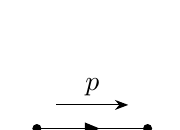
\begin{tikzpicture}[baseline = (r.base)]
        \begin{feynman}[inline = (r.base)]
          \vertex[dot] (x) {};
          \vertex[right=4em of x, dot] (y) {};

          \vertex[below=0.2em of x] (r) {};

          \diagram* {
            (x) -- [fermion, momentum = \(p\)] (y),
          };
        \end{feynman}
      \end{tikzpicture}
      \,=\, \tilde{S}_\text{D}(p)
      $;
    \end{enumerate}
  \item vertex:
    $
    \begin{tikzpicture}[baseline = (r.base)]
      \begin{feynman}[inline = (r.base)]
        \vertex[dot] (x) {};
        \vertex[right=4em of x] (y) {};

        \vertex[above=2em of x] (p) {};
        \vertex[left=2em of p] (p1) {};
        \vertex[below=4em of p1] (p2) {};

        \vertex (l1) at ($(y)+(0.4,0)$) {\(\mu\)};

        \vertex[below=0.2em of x] (r) {};

        \diagram* {
          (x) -- [photon] (y),
          (p2) -- [fermion] (x) -- [fermion] (p1),
        };
      \end{feynman}
    \end{tikzpicture}
    \,=\, -i e \gamma^\mu
    $;
  \item external legs:
    \begin{enumerate}
      \item initial state:
        \begin{enumerate}
          \item vector:
            $
            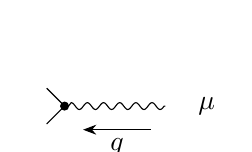
\begin{tikzpicture}[baseline = (r.base)]
              \begin{feynman}[inline = (r.base)]
                \vertex[dot] (x) {};
                \vertex[right=4em of x] (y) {};

                \vertex[above=1em of x] (p) {};
                \vertex[left=1em of p] (p1) {};
                \vertex[below=2em of p1] (p2) {};

                \vertex (l1) at ($(y)+(0.4,0)$) {\(\mu\)};

                \vertex[below=0.2em of x] (r) {};

                \diagram* {
                  (y) -- [photon, momentum = \(q\)] (x),
                  (p2) -- (x) -- (p1),
                };
              \end{feynman}
            \end{tikzpicture}
            \,=\, \epsilon_\mu(q)
            $;
          \item fermion:
            $
            \begin{tikzpicture}[baseline = (r.base)]
              \begin{feynman}[inline = (r.base)]
                \vertex[dot] (x) {};
                \vertex[right=4em of x] (y) {};

                \vertex[above=1em of x] (p) {};
                \vertex[left=1em of p] (p1) {};
                \vertex[below=2em of p1] (p2) {};

                \vertex[below=0.2em of x] (r) {};

                \diagram* {
                  (y) -- [fermion, momentum = \(p\)] (x),
                  (p2) -- (x) -- (p1),
                };
              \end{feynman}
            \end{tikzpicture}
            \,=\, u^s(p)
            $;
          \item anti-fermion:
            $
            \begin{tikzpicture}[baseline = (r.base)]
              \begin{feynman}[inline = (r.base)]
                \vertex[dot] (x) {};
                \vertex[right=4em of x] (y) {};

                \vertex[above=1em of x] (p) {};
                \vertex[left=1em of p] (p1) {};
                \vertex[below=2em of p1] (p2) {};

                \vertex[below=0.2em of x] (r) {};

                \diagram* {
                  (y) -- [anti fermion, momentum = \(k\)] (x),
                  (p2) -- (x) -- (p1),
                };
              \end{feynman}
            \end{tikzpicture}
            \,=\, \bar{v}^s(k)
            $;
        \end{enumerate}
      \item final state:
        \begin{enumerate}
          \item scalar:
            $
            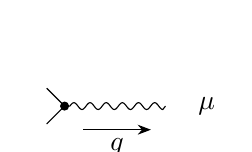
\begin{tikzpicture}[baseline = (r.base)]
              \begin{feynman}[inline = (r.base)]
                \vertex[dot] (x) {};
                \vertex[right=4em of x] (y) {};

                \vertex[above=1em of x] (p) {};
                \vertex[left=1em of p] (p1) {};
                \vertex[below=2em of p1] (p2) {};

                \vertex (l1) at ($(y)+(0.4,0)$) {\(\mu\)};

                \vertex[below=0.2em of x] (r) {};

                \diagram* {
                  (x) -- [photon, momentum' = \(q\)] (y),
                  (p2) -- (x) -- (p1),
                };
              \end{feynman}
            \end{tikzpicture}
            \,=\, \epsilon_\mu^*(q)
            $;
          \item fermion:
            $
            \begin{tikzpicture}[baseline = (r.base)]
              \begin{feynman}[inline = (r.base)]
                \vertex[dot] (x) {};
                \vertex[right=4em of x] (y) {};

                \vertex[above=1em of x] (p) {};
                \vertex[left=1em of p] (p1) {};
                \vertex[below=2em of p1] (p2) {};

                \vertex[below=0.2em of x] (r) {};

                \diagram* {
                  (x) -- [fermion, momentum' = \(p\)] (y),
                  (p2) -- (x) -- (p1),
                };
              \end{feynman}
            \end{tikzpicture}
            \,=\, \bar{u}^s(p)
            $;
          \item anti-fermion:
            $
            \begin{tikzpicture}[baseline = (r.base)]
              \begin{feynman}[inline = (r.base)]
                \vertex[dot] (x) {};
                \vertex[right=4em of x] (y) {};

                \vertex[above=1em of x] (p) {};
                \vertex[left=1em of p] (p1) {};
                \vertex[below=2em of p1] (p2) {};

                \vertex[below=0.2em of x] (r) {};

                \diagram* {
                  (x) -- [anti fermion, momentum' = \(k\)] (y),
                  (p2) -- (x) -- (p1),
                };
              \end{feynman}
            \end{tikzpicture}
            \,=\, v^s(k)
            $;
        \end{enumerate}
    \end{enumerate}
  \item impose momentum conservation at each vertex;
  \item integrate over each undetermined loop momentum $ p $ with measure $ \frac{\dd^4p}{(2\pi)^4} $ (each closed fermionic loop determines an additional $ (-1) $ factor due to anti-commutation);
  \item divide by the symmetry factor of the diagram.
\end{enumerate}
Of course, when considering fermions with charge $ Q $ (in units of $ \abs{e} $), substitute $ e \mapsto Q\abs{e} $ in the above formulae. \\
It can be shown that the interaction mediated by a vector field is attractive for $ f\bar{f} $ scattering and repulsive for $ ff $ and $ \bar{f} \bar{f} $ scattering.












\clearpage
\bookmarksetupnext{level = -1}
\pagestyle{biblio}
\printbibliography[heading = bibintoc, title = {Bibliography}]

\end{document}
